% Options for packages loaded elsewhere
\PassOptionsToPackage{unicode,linktoc=all}{hyperref}
\PassOptionsToPackage{hyphens}{url}
%
\documentclass[
  letterpaper,
]{krantz}

\usepackage{amsmath,amssymb}
\usepackage{iftex}
\ifPDFTeX
  \usepackage[T1]{fontenc}
  \usepackage[utf8]{inputenc}
  \usepackage{textcomp} % provide euro and other symbols
\else % if luatex or xetex
  \usepackage{unicode-math}
  \defaultfontfeatures{Scale=MatchLowercase}
  \defaultfontfeatures[\rmfamily]{Ligatures=TeX,Scale=1}
\fi
\usepackage{lmodern}
\ifPDFTeX\else  
    % xetex/luatex font selection
  \setmonofont[Scale=0.66]{Roboto Mono}
\fi
% Use upquote if available, for straight quotes in verbatim environments
\IfFileExists{upquote.sty}{\usepackage{upquote}}{}
\IfFileExists{microtype.sty}{% use microtype if available
  \usepackage[]{microtype}
  \UseMicrotypeSet[protrusion]{basicmath} % disable protrusion for tt fonts
}{}
\makeatletter
\@ifundefined{KOMAClassName}{% if non-KOMA class
  \IfFileExists{parskip.sty}{%
    \usepackage{parskip}
  }{% else
    \setlength{\parindent}{0pt}
    \setlength{\parskip}{6pt plus 2pt minus 1pt}}
}{% if KOMA class
  \KOMAoptions{parskip=half}}
\makeatother
\usepackage{xcolor}
\setlength{\emergencystretch}{3em} % prevent overfull lines
\setcounter{secnumdepth}{5}
% Make \paragraph and \subparagraph free-standing
\ifx\paragraph\undefined\else
  \let\oldparagraph\paragraph
  \renewcommand{\paragraph}[1]{\oldparagraph{#1}\mbox{}}
\fi
\ifx\subparagraph\undefined\else
  \let\oldsubparagraph\subparagraph
  \renewcommand{\subparagraph}[1]{\oldsubparagraph{#1}\mbox{}}
\fi


\providecommand{\tightlist}{%
  \setlength{\itemsep}{0pt}\setlength{\parskip}{0pt}}\usepackage{longtable,booktabs,array}
\usepackage{calc} % for calculating minipage widths
% Correct order of tables after \paragraph or \subparagraph
\usepackage{etoolbox}
\makeatletter
\patchcmd\longtable{\par}{\if@noskipsec\mbox{}\fi\par}{}{}
\makeatother
% Allow footnotes in longtable head/foot
\IfFileExists{footnotehyper.sty}{\usepackage{footnotehyper}}{\usepackage{footnote}}
\makesavenoteenv{longtable}
\usepackage{graphicx}
\makeatletter
\def\maxwidth{\ifdim\Gin@nat@width>\linewidth\linewidth\else\Gin@nat@width\fi}
\def\maxheight{\ifdim\Gin@nat@height>\textheight\textheight\else\Gin@nat@height\fi}
\makeatother
% Scale images if necessary, so that they will not overflow the page
% margins by default, and it is still possible to overwrite the defaults
% using explicit options in \includegraphics[width, height, ...]{}
\setkeys{Gin}{width=\maxwidth,height=\maxheight,keepaspectratio}
% Set default figure placement to htbp
\makeatletter
\def\fps@figure{htbp}
\makeatother
% definitions for citeproc citations
\NewDocumentCommand\citeproctext{}{}
\NewDocumentCommand\citeproc{mm}{%
  \begingroup\def\citeproctext{#2}\cite{#1}\endgroup}
\makeatletter
 % allow citations to break across lines
 \let\@cite@ofmt\@firstofone
 % avoid brackets around text for \cite:
 \def\@biblabel#1{}
 \def\@cite#1#2{{#1\if@tempswa , #2\fi}}
\makeatother
\newlength{\cslhangindent}
\setlength{\cslhangindent}{1.5em}
\newlength{\csllabelwidth}
\setlength{\csllabelwidth}{3em}
\newenvironment{CSLReferences}[2] % #1 hanging-indent, #2 entry-spacing
 {\begin{list}{}{%
  \setlength{\itemindent}{0pt}
  \setlength{\leftmargin}{0pt}
  \setlength{\parsep}{0pt}
  % turn on hanging indent if param 1 is 1
  \ifodd #1
   \setlength{\leftmargin}{\cslhangindent}
   \setlength{\itemindent}{-1\cslhangindent}
  \fi
  % set entry spacing
  \setlength{\itemsep}{#2\baselineskip}}}
 {\end{list}}
\usepackage{calc}
\newcommand{\CSLBlock}[1]{\hfill\break\parbox[t]{\linewidth}{\strut\ignorespaces#1\strut}}
\newcommand{\CSLLeftMargin}[1]{\parbox[t]{\csllabelwidth}{\strut#1\strut}}
\newcommand{\CSLRightInline}[1]{\parbox[t]{\linewidth - \csllabelwidth}{\strut#1\strut}}
\newcommand{\CSLIndent}[1]{\hspace{\cslhangindent}#1}

\pagenumbering{arabic}
\usepackage{makeidx}
\usepackage{lscape}
\newcommand{\blandscape}{\begin{landscape}}
\newcommand{\elandscape}{\end{landscape}}
\makeatletter
\makeindex
\makeatother
\makeatletter
\@ifpackageloaded{tcolorbox}{}{\usepackage[skins,breakable]{tcolorbox}}
\@ifpackageloaded{fontawesome5}{}{\usepackage{fontawesome5}}
\definecolor{quarto-callout-color}{HTML}{909090}
\definecolor{quarto-callout-note-color}{HTML}{0758E5}
\definecolor{quarto-callout-important-color}{HTML}{CC1914}
\definecolor{quarto-callout-warning-color}{HTML}{EB9113}
\definecolor{quarto-callout-tip-color}{HTML}{00A047}
\definecolor{quarto-callout-caution-color}{HTML}{FC5300}
\definecolor{quarto-callout-color-frame}{HTML}{acacac}
\definecolor{quarto-callout-note-color-frame}{HTML}{4582ec}
\definecolor{quarto-callout-important-color-frame}{HTML}{d9534f}
\definecolor{quarto-callout-warning-color-frame}{HTML}{f0ad4e}
\definecolor{quarto-callout-tip-color-frame}{HTML}{02b875}
\definecolor{quarto-callout-caution-color-frame}{HTML}{fd7e14}
\makeatother
\makeatletter
\@ifpackageloaded{bookmark}{}{\usepackage{bookmark}}
\makeatother
\makeatletter
\@ifpackageloaded{caption}{}{\usepackage{caption}}
\AtBeginDocument{%
\ifdefined\contentsname
  \renewcommand*\contentsname{Table of contents}
\else
  \newcommand\contentsname{Table of contents}
\fi
\ifdefined\listfigurename
  \renewcommand*\listfigurename{List of Figures}
\else
  \newcommand\listfigurename{List of Figures}
\fi
\ifdefined\listtablename
  \renewcommand*\listtablename{List of Tables}
\else
  \newcommand\listtablename{List of Tables}
\fi
\ifdefined\figurename
  \renewcommand*\figurename{Figure}
\else
  \newcommand\figurename{Figure}
\fi
\ifdefined\tablename
  \renewcommand*\tablename{Table}
\else
  \newcommand\tablename{Table}
\fi
}
\@ifpackageloaded{float}{}{\usepackage{float}}
\floatstyle{ruled}
\@ifundefined{c@chapter}{\newfloat{codelisting}{h}{lop}}{\newfloat{codelisting}{h}{lop}[chapter]}
\floatname{codelisting}{Listing}
\newcommand*\listoflistings{\listof{codelisting}{List of Listings}}
\makeatother
\makeatletter
\makeatother
\makeatletter
\@ifpackageloaded{caption}{}{\usepackage{caption}}
\@ifpackageloaded{subcaption}{}{\usepackage{subcaption}}
\makeatother
\makeatletter
\@ifpackageloaded{tcolorbox}{}{\usepackage[skins,breakable]{tcolorbox}}
\makeatother
\makeatletter
\@ifundefined{shadecolor}{\definecolor{shadecolor}{rgb}{.97, .97, .97}}{}
\makeatother
\makeatletter
\@ifundefined{codebgcolor}{\definecolor{codebgcolor}{HTML}{FAFAFA}}{}
\makeatother
\makeatletter
\ifdefined\Shaded\renewenvironment{Shaded}{\begin{tcolorbox}[colback={codebgcolor}, sharp corners, boxrule=0pt, frame hidden, enhanced, breakable]}{\end{tcolorbox}}\fi
\makeatother
\ifLuaTeX
  \usepackage{selnolig}  % disable illegal ligatures
\fi
\usepackage{bookmark}

\IfFileExists{xurl.sty}{\usepackage{xurl}}{} % add URL line breaks if available
\urlstyle{same} % disable monospaced font for URLs
% Make links footnotes instead of hotlinks:
\DeclareRobustCommand{\href}[2]{#2\footnote{\url{#1}}}
\hypersetup{
  pdftitle={Models Demystified},
  pdfauthor={Michael Clark \& Seth Berry},
  hidelinks,
  pdfcreator={LaTeX via pandoc}}

\title{Models Demystified}
\usepackage{etoolbox}
\makeatletter
\providecommand{\subtitle}[1]{% add subtitle to \maketitle
  \apptocmd{\@title}{\par {\large #1 \par}}{}{}
}
\makeatother
\subtitle{A Practical Guide from t-tests to Deep Learning}
\author{Michael Clark \& Seth Berry}
\date{}

\begin{document}
\maketitle

\pagenumbering{roman}

\renewcommand*\contentsname{Contents}
{
\setcounter{tocdepth}{2}
\tableofcontents
}
\bookmarksetup{startatroot}

\chapter*{Preface}\label{preface}
\addcontentsline{toc}{chapter}{Preface}

\markboth{Preface}{Preface}

TODO: Quarto bug prints this twice in ToC; tried various header tricks
to no avail. Also, not unnumbered by default for krantz.cls.

Hi there, this is our book! It's about models great and small, and we
hope you'll find some useful things here. Our main goal is to provide a
resource for people who are learning about models, and we hope that it
will be useful for people who are just starting out, as well as for
people who are already familiar with models but want to learn from a
different perspective. Whether you're a machine learning master that
would like a little bit more statistical nuance, or an academic trying
to dive into the world of machine learning, we hope you'll find it
helpful.

You'll definitely want tok have some familiarity with R or Python, and
some basic knowledge of statistics will be helpful. We'll try to explain
things as we go, but we won't be able to cover everything. If you're
looking for a good introduction to R, we recommend
\href{https://r4ds.had.co.nz/}{R for Data Science} or the
\href{https://jakevdp.github.io/PythonDataScienceHandbook/}{Python Data
Science Handbook} for Python. Beyond that, we'll try to provide the
context you need. We're not here to make you an expert, just to help you
get acquainted with the world of models.

\section*{Acknowledgments}\label{acknowledgments}
\addcontentsline{toc}{section}{Acknowledgments}

\markright{Acknowledgments}

A lot of people helped when writing the book\ldots{}

\bookmarksetup{startatroot}

\chapter*{Introduction}\label{introduction}
\addcontentsline{toc}{chapter}{Introduction}

\markboth{Introduction}{Introduction}

\pagenumbering{arabic}

Regardless of background, and whether we're conscious of it or not, we
are constantly inundated with data. It's inescapable, from our first
attempts to understand the world around us, to our most recent efforts
to explain why we still don't get it. Even now, our most complicated and
successful models are almost uninterpretable even to those that created
them. But that doesn't mean that even in those cases we can't understand
the essence of how they work. And if you're reading this, you are
probably the type of person that wants to keep trying! So for seasoned
professionals or perhaps just the data curious, we want to help you
learn more about how to use data to answer the questions you have.

\section*{What Is This Book?}\label{what-is-this-book}
\addcontentsline{toc}{section}{What Is This Book?}

\markright{What Is This Book?}

This book is a practical resource, something we hope you can refer to
for a quick overview of a specific modeling technique, a reminder of
something you've seen before, or perhaps a sneak peak into some modeling
details. The text is focused on a few statistical and machine learning
approaches that are widely employed, and specifically those which form
the basis for most other models in use. Believe it or not, whether a
lowly \emph{t}-test or a complex neural network, there is a tie that
binds. We hope to help you understand some of the core modeling
principles, and how the simpler models can be extended and applied to a
wide variety of data scenarios.

Our approach here is first and foremost a practical one, as models
themselves are just tools to help us reach a goal. If a model doesn't
work in the world, it's not very useful. But modeling is often a
delicate balance of interpretation and prediction, and each data
situation is unique in some way, requiring a bespoke approach. What
works well in one setting may be poor in another, and what may be the
state of the art may only be marginally better than a notably simpler
approach that is far more interpretable. In addition, complexities arise
even in an otherwise deceptively simple application. However, if you
have the core understanding of the techniques that lie at the heart of
many models, you'll automatically have many more tools at your disposal
to tackle the problems you face, and be more comfortable with choosing
the best for your needs.

\section*{Who Should Use This Book?}\label{who-should-use-this-book}
\addcontentsline{toc}{section}{Who Should Use This Book?}

\markright{Who Should Use This Book?}

This book is intended for every type of \emph{data dabbler}, no matter
what part of the data world you call home. If you consider yourself a
data scientist, a business analyst, or a statistical hobbyist, you
already know that the best part of a good dive into data is the
modeling. But whatever your data persuasion, models give us the
possibility to answer questions, make predictions, and understand what
we're interested in a little bit better. And no matter who you are, it
isn't always easy to understand \emph{how the models work}. Even when
you do get a good grasp of a modeling approach, it can still get
complicated, and there are a lot of details to keep track of. In other
cases, maybe you just have other things going on in your life and have
forgotten a few things. We find that it's always good to remind yourself
of the basics! So if you're just interested in data and hoping to
understand it a little better, then it's likely you'll find something
useful in this book!

Your humble authors have struggled mightily themselves throughout the
course of their data history, and still do! We were initially taught by
those that weren't exactly experts, and often found it difficult to get
a good grasp of statistical modeling and machine learning. We've had to
learn how to use the tools, how to interpret the results, and possibly
the most difficult, how to explain what we're doing to others! We've
forgotten a lot, confused ourselves, and made some happy accidents in
the process. That's okay! Our goal here is to help you avoid some of
those pitfalls, help you understand the basics of how models work, and
get a sense of how most modeling endeavors have a lot of things in
common.

Whether you enthusiastically pour over formulas and code, or prefer to
skip over them, we promise that you don't need to memorize a formula to
get a good understanding of modeling and related issues. We are the
first to admit that we have long dumped the ability to pull formulas out
of our brain folds\footnote{We actually never had this ability.};
however, knowing how those individual pieces work together only helps to
deepen your understanding of the model. Typically using code puts the
formula into more concrete terms that you can then use in different ways
to solidify and expand your knowledge. Sometimes you just need a
reminder or want to see what function you'd use. And often, the
visualization will reveal even more about what's going than the formula
or the code. In short, there are a lot of tools at your disposal to help
learn modeling in a way that works for you. We hope that anyone that
would be interested in the book will find a way to learn things in a
manner that suits them best.

There is bit of a caveat. We aren't going to teach you basic statistics
or how to program in R or Python. Although there is a good chance you
will learn some of it here, you'll have an easier time if you have a
very basic understanding of statistics and some familiarity with coding.
We will provide some resources for you to learn more about these topics,
but we won't be covering them in detail. The (\textbf{appendix?}) will
provide some more information about prerequisites or just stuff that
would be good to know. However, we really aren't assuming a lot of
conceptual knowledge, and are, if anything, assuming that whatever
knowledge you have may be a bit loose or fuzzy. That's okay!

\section*{What Can You Expect?}\label{what-can-you-expect}
\addcontentsline{toc}{section}{What Can You Expect?}

\markright{What Can You Expect?}

For each model that we cover, you can expect the following in terms of
content:

\begin{itemize}
\tightlist
\item
  Overview

  \begin{itemize}
  \tightlist
  \item
    Why it's useful
  \item
    Conceptual example and interpretation
  \item
    Where the model lies in the grand scheme of topics that we will
    cover
  \end{itemize}
\item
  Key ideas and concepts

  \begin{itemize}
  \tightlist
  \item
    Brief summary and definition list of concepts or terms
  \end{itemize}
\item
  Demonstration with data, code, results, and visualizations

  \begin{itemize}
  \tightlist
  \item
    The data will often be simulations as that opens doors for further
    understanding, or a dataset that hopefully is a little more
    interesting than mtcars or iris.
  \item
    The demonstrations will provide you the opportunity to get your
    hands as dirty as you wish. We will present the code in two ways:

    \begin{itemize}
    \tightlist
    \item
      standard functions (e.g., \texttt{lm} in R, \texttt{ols} in
      \texttt{statsmodels} for Python)
    \item
      the steps to recreate the estimation process on your own (or at
      least something a little more hands-on)
    \end{itemize}
  \end{itemize}
\item
  Commentary, cautions, and where to explore next
\end{itemize}

We are taking this approach for one reason: so that you can go as deep
as you wish. If you are looking for a quick tutorial on helpful models,
then you might not find yourself going any deeper than the standard
functions (or even getting into the code at all). If you want to really
dive into these models, then you might find yourself working through the
complete steps. Another approach is to allow yourself some time between
the standard functions and complete steps. You could work through the
standard functions of every chapter, give it some time to marinate, and
then work back through the complete steps. While we certainly recommend
working through the chapters in order, we want to give you the
flexibility to choose your own depth within each.

We hope that this book can serve as a ``choose your own adventure''
statistical reference. Whether you want a surface-level understanding, a
deeper dive, or just want to be able to understand what the analysts in
your organization are talking about, you will find value in this book.
While we assume that you have a basic familiarity with coding, that
doesn't mean that you need to work through every line of code to
understand the fundamental principles and use cases of every model.

\section*{Which Language?}\label{which-language}
\addcontentsline{toc}{section}{Which Language?}

\markright{Which Language?}

You've probably noticed most books, blogs, and courses on data science
choose R or Python. While many individuals often take an opinionated
approach towards teaching and using one over the other, we eschew
dogmatic approaches and language flame wars. R and Python are both great
languages (and equally flawed in unique ways), and it is advantageous to
be knowledgeable of both, even if you focus on one specifically, as they
are the most popular languages for statistical modeling and machine
learning. We use both extensively in our own work for teaching, personal
use, and production level code, and have found both are up to whatever
task you have in mind. Throughout this book, we will be presenting
demonstrations in both R and Python, and you can use both or take your
pick, but we want to leave that choice up to you. Our goal isn't to
obscure the ideas behind packages and specialty functions or tell you
why one languages is superior to the other (they aren't), but to show
you the most basic functions behind big model ideas.

While we want to provide you choice, we truly hope that displaying both
languages can help people to ``convert'' from one to the other. We have
spent countless hours, slumped over our computers, debugging errors and
figuring things out. If we can take away one source of pain for you,
that would be great! We'd like to consider this as a resource for the R
user, who knows exactly what they want to do in R, but could use a
little help translating their R knowledge to Python; we'd also like this
book to be a resource for the Python user, who sees the value in R's
statistical modeling abilities.

\section*{Choose Your Own Adventure}\label{choose-your-own-adventure}
\addcontentsline{toc}{section}{Choose Your Own Adventure}

\markright{Choose Your Own Adventure}

As an example of how things will go, let's look at the different ways we
might express a relationship between two variables. If you want just a
little bit of background, you can read through the \emph{Overview} and
\emph{Key Ideas}. If you want to see the easy way to use the model, you
can work through the \emph{Standard Function} section. If you want to
see the method from start to finish, feel free to work through the
\emph{Roll Your Own} section. If all of that sounds like a lot of work
and you'd rather look at the pretty pictures, that's fine
too\footnote{We love pretty pictures too! Sometimes it's the best way to
  bring a lot of ideas together.}, just jump to the \emph{Visualization}
section.

\subsection*{Overview}\label{overview}
\addcontentsline{toc}{subsection}{Overview}

Correlations provide a means of understanding how, and \emph{if}, two or
more things are related. For any two variables or features, we can
estimate a single value that signals the strength and direction of the
relationship between them. Despite limitations, correlations can be a
great way to get a quick understanding of the relationship between two
features. One variable could be temperature while another variable is
the number of ice cream cones sold, or one is the number of hours spent
studying and another variable is the grade on a test, maybe the number
of hours spent watching TV versus the number of hours spent exercising.
The correlation value will give us information that is similarly
interpretable in each case.

\subsection*{Key Ideas}\label{key-ideas}
\addcontentsline{toc}{subsection}{Key Ideas}

Here are key ideas to consider for understanding correlation.

\begin{itemize}
\tightlist
\item
  \textbf{Variance}: Two variables must vary if they are to
  \emph{co-}vary
\item
  \textbf{Covariance}: Joint variability of two variables, i.e.~how they
  vary together
\item
  \textbf{Interpretation}: Covariance is hard to interpret because the
  variables are typically on different scales
\item
  \textbf{Correlation}: Correlation is a standardized covariance, so it
  is easier to interpret
\end{itemize}

Another way to think about correlation is through the lens of
\emph{variance} \emph{covariance}. Covariance is a measure of the joint
variability of two variables, i.e.~how they \emph{vary} together. If two
variables are highly correlated, then they have a high degree of
covariance, i.e.~they vary together in a meaningful way.

\subsection*{Demonstration}\label{demonstration}
\addcontentsline{toc}{subsection}{Demonstration}

To demonstrate correlation, we could start by formally defining it. Here
is a formula for the Pearson-Product-Moment correlation coefficient.
What everyone typically just calls ``correlation'' or Pearson's \emph{r}
is actually the \emph{Pearson Product-Moment Correlation} -- that is a
lot of words, though, so we will just go with correlation. As we
mentioned earlier, we want to give you the choice to dive in as deep as
you want.

\begin{equation}\phantomsection\label{eq-pearson}{
\rho = \frac{\Sigma(x_i-\bar{x})(y_i-\bar{y})}{\sqrt{\Sigma(x_i-\bar{x})^2\Sigma(y_i-\bar{y})^2}}
}\end{equation}

In words, starting with the numerator, we are going to subtract the mean
of \emph{x} from every observation of \emph{x}, do the same for
\emph{y}, multiply them together, and then sum them to produce a single
value. If you've taken a statistics class before, you might have seen
this part of the formula when talking about \emph{covariance} -- the
joint variability of two variables. In fact, if you just divide the
numerator by n-1 you'd get the covariance value. Covariance values,
though, are not standardized; therefore, they are a bit tough to
interpret. You will get a sign indicating relationship (just like a
correlation) and the magnitude tells you the strength of the
relationship, but it is hard to get your head around how much stronger a
covariance of 4.00 is compared to a covariance of 0.28.

This is where the denominator comes into play. To put it into real
terms, we will subtract the mean of \emph{x} from every observation of
\emph{x} (i.e.~get the deviations of x), square those values, and sum
those values to produce a single value. We will do the same for
\emph{y}, multiply those results, and then take the square root of that
product. The denominator might also look familiar to some. The
individual pieces- \(\Sigma(x_i-\bar{x})^2\) and
\(\Sigma(y_i-\bar{y})^2\) - are computing the \emph{variance} of x and
y. Taking the square root of variance gives us the \emph{standard
deviation}. Basically, we're getting a combined standard deviation to
scale the covariance. Using the standard deviation will mitigate the
effects of \emph{x} and \emph{y} potentially being on different scales;
in other words, we want to know how much two variables move together,
even if the means and typical movement (deviation) might be very
different.

Here is a simplification, depicting correlation as a
\textbf{standardized covariance}.

\begin{equation}\phantomsection\label{eq-corcov}{
\rho = \frac{cov(x,y)}{\sigma_x\sigma_y}
}\end{equation}

where \(cov(x,y)\) is the covariance between \(x\) and \(y\), and
\(\sigma_x\) and \(\sigma_y\) are the standard deviations of \(x\) and
\(y\), respectively. So putting it all together, we are simply looking
at the ratio of raw covariance (i.e., how much two variables ``move''
together) and standard deviation (i.e., the amount of dispersion within
a variable). Just as we mentioned earlier, simpler concepts often tie
models together! What might look like a tricky formula, really just
starts with means and deviations, variance and covariance!

As a reminder, this correlation will give us an idea about the
\textbf{linear relationship} between two continuous variables; we will
get a value between -1 and 1, with values closer to 0 indicating that
there is no linear relationship between the two variables. As values get
closer to 1, we have a \textbf{positive correlation} -- as values for
one variable increase, values for the other variable tend to increase
along with it. As the correlation gets closer to -1, we have a
\textbf{negative correlation} -- as values for one variable increase,
values for the other variable typically decrease. Correlations can be
useful for quickly exploring linear relationships, but let's not get too
excited about it -- they aren't going to help you answer any big
questions! We also don't want to get too carried away with ``statistical
significance'' yet -- once samples get large, even small correlations
become ``significant''. Instead, just use correlations to explore the
patterns within your data, start getting ideas about interesting
relationships that you might find, and leave worries about significance
for people with more time on their hands.

\subsubsection*{Code}\label{code}
\addcontentsline{toc}{subsubsection}{Code}

It's often easier to understand a concept by seeing it in action. So
let's start by creating some data. We'll create a variable \texttt{x},
then make a \texttt{y} that will have a linear relationship with it, but
also have some random noise. We'll then plot the two variables to see
what they look like. To help your understanding, fiddle with the knobs
noted.

\subsubsection{R}

\begin{verbatim}
set.seed(seed = 1001)
N = 500
x = rnorm(n = N, mean = 0, sd = 1)

# Fiddle with the .5 and .75.
# The first can also be negative if you like!
y = .5 * x + rnorm(n = N, mean = 0, sd = .75)
\end{verbatim}

\subsubsection{Python}

\begin{verbatim}
import numpy as np

np.random.seed(seed = 1001)
N = 500
x = np.random.normal(loc = 0, scale = 1, size = N)

# Fiddle with the .5 and .75. 
# The first can also be negative if you like!
y = .5*x + np.random.normal(loc = 0, scale = .75, size = N) 
\end{verbatim}

Now check out the plot of those two values:

\begin{figure}[H]

{\centering \includegraphics{introduction_files/figure-pdf/cor_viz-1.pdf}

}

\caption{Scatterplot of two variables.}

\end{figure}%

Remember that correlation is testing for the presence of a linear
relationship, with -1 indicating a perfect negative relationship, 1
indicating a perfect positive relationship, and 0 indicating no
relationship. Before we see the actual correlation value for these two
variables, take a guess as to what value we are going to get!

Before we create our own function, we can use R's \texttt{cor} function
or numpy's \texttt{corrcoef} function. You should get something around
0.6.

\begin{verbatim}
# Results for R and Python will be slightly
# different due to different random number generators
cor(x, y)
np.corrcoef(x, y)
\end{verbatim}

\begin{verbatim}
[1] 0.557
\end{verbatim}

When you guessed the value, were you close? If so, congrats! If not, try
fiddling with those knobs noted until things get a little clearer. But
now that we already know the answer, let's make sure that we can get the
same answer by working through the formula via code. The following takes
that initial formula approach and turns it into a function that we can
use to compute the correlation between any two variables. We'll then use
that function to compute the correlation between our \texttt{x} and
\texttt{y} variables.

\subsubsection{R}

\begin{verbatim}
my_cor = function(x, y) {
    # First, we need to compute the averages for x and y.
    # The rest follows the formula.
    x_bar = mean(x)
    y_bar = mean(y)

    numerator = sum((x - x_bar) * (y - y_bar))

    denominator = sqrt(
        sum((x - x_bar)^2) * sum((y - y_bar)^2)
    )

    numerator / denominator
}

# using the builtin functions
my_cor2 = function(x, y) {
    cov(x, y) / (sd(x) * sd(y))
}

my_cor(x, y)
\end{verbatim}

\begin{verbatim}
[1] 0.557
\end{verbatim}

\subsubsection{Python}

\begin{verbatim}
def my_cor(x, y):
  # First, we need to compute the averages for x and y.
  # The rest follows the formula.
    x_bar = np.mean(x)
    y_bar = np.mean(y)
    
    numerator = np.sum((x - x_bar) * (y - y_bar))
    
    denominator = np.sqrt(
      np.sum((x - x_bar)**2) * np.sum((y - y_bar)**2)
    )

    # We will finish by dividing the numerator by the 
    # denominator.
    # This will ensure that we have a value between -1 and 1.
    return(numerator / denominator)

my_cor(x, y)
\end{verbatim}

\begin{verbatim}
0.5390318454354402
\end{verbatim}

It doesn't matter which language we use, the steps are largely the same
when we break it down into the individual pieces!

\subsection*{Visualization}\label{visualization}
\addcontentsline{toc}{subsection}{Visualization}

A long time ago, in a land far away, the authors of this book worked
together to help clients traverse the forests of data to reach their
modeling goals. While there were many great learning opportunities along
the way, working with clients showed us the kinds of help that people
really needed in adventuring with data and models. Even so, there were
many requests that made us grimace, and one stood atop Mount Ridiculous:
to produce a correlation matrix with 115 variables and export that
matrix to a spreadsheet. We still don't recommend such shenanigans, but
there are ways to try and understand correlation matrices. Since we were
in the business of helping people do their work better, one way we often
did so was via a \emph{corrplot}.

We'll start with a something manageable. We create a data set with six
variables of two sets: a, b , c, and x, y, z, and then we can take a
quick look at the correlation matrix.

\begin{longtable}{lrrrrrr}
\caption{Correlation matrix}\tabularnewline

\toprule
feature & a & b & c & x & y & z \\ 
\midrule\addlinespace[2.5pt]
a & $1.00$ & $0.46$ & $0.45$ & $-0.16$ & $-0.21$ & $-0.19$ \\ 
b & $0.46$ & $1.00$ & $0.49$ & $-0.07$ & $-0.18$ & $-0.14$ \\ 
c & $0.45$ & $0.49$ & $1.00$ & $-0.16$ & $-0.23$ & $-0.20$ \\ 
x & $-0.16$ & $-0.07$ & $-0.16$ & $1.00$ & $0.49$ & $0.48$ \\ 
y & $-0.21$ & $-0.18$ & $-0.23$ & $0.49$ & $1.00$ & $0.52$ \\ 
z & $-0.19$ & $-0.14$ & $-0.20$ & $0.48$ & $0.52$ & $1.00$ \\ 
\bottomrule
\end{longtable}

Now we have the \emph{pairwise correlations} between all six of our
variables, with 1's on the diagonals (naturally, a variable has a
perfect correlation with itself). You can check out the lower diagonal
or the upper diagonal, because they contain the exact same information.
Quickly, though, find the interesting pattern in that matrix!

Producing the correlations between just 6 variables gives us 15
correlation coefficients to examine! You can see that you'll need to
spend more than a few seconds on finding the interesting patterns within
the data (or if there are any patterns at all). Our brains are oriented
towards vision, so we can use \emph{preattentive processing} elements,
like hue, saturation, and size, to make finding interesting patterns
easier.

Since we already have a correlation matrix, we can use various means to
find those patterns, which include visualizing the matrix itself,
network graphs and others. Here is one way to do it.

\begin{tcolorbox}[enhanced jigsaw, opacityback=0, leftrule=.75mm, bottomrule=.15mm, colframe=quarto-callout-note-color-frame, rightrule=.15mm, breakable, left=2mm, colback=white, arc=.35mm, toprule=.15mm]

Some recommended R packages for visualizing a correlation matrix include
\texttt{corrr}, \texttt{ggcor}, and \texttt{corrplot}. For python, one
has options for \texttt{seaborn}, \texttt{pandas}, \texttt{biokit}, and
others.

\end{tcolorbox}

\begin{figure}[H]

{\centering \includegraphics{introduction_files/figure-pdf/corrplot_demo-1.pdf}

}

\caption{Correlation matrix visualization}

\end{figure}%

Let's break down what we're seeing just a little bit. The lower triangle
has the correlation values. It adds information, though, by changing the
hue by correlation value -- red for negative values and blue for
positive values -- and increasing the saturation as the correlation
value becomes stronger. The upper triangle contains the same
information, but the size of the circle is tied directly to the strength
of the correlation. You'll also notice that the weaker correlations are
more hidden in the visualization, allowing us to focus only on those
interesting relationships.

What do you think? Was it easier to spot the points of interest? It
looks like there is an a-b-c group and x-y-z group that are similarly
correlated within their respective groups. We can also see that the
a-b-c group is negatively correlated with the x-y-z group. Visualizing
the correlation matrix can usually make it easier to find those
interesting patterns.

\subsection*{Commentary}\label{commentary}
\addcontentsline{toc}{subsection}{Commentary}

The correlation is a starting point for understanding linear models,
which serve as the foundation for modeling in general. It is very
limited by only assessing linear relationships between variables, as
well as only pairwise relationships. Other metrics can overcome these,
but they have their own limitations. The basic Pearson-Product-Moment
correlation coefficient is still the most widely used and a typical
starting point in many data adventures.

Things to explore further next:

\begin{itemize}
\tightlist
\item
  Rank correlation (e.g., Spearman's rho, Kendall's tau)
\item
  Distance metrics (e.g., euclidean, manhattan, cosine)
\item
  Non-linear relationships and interactions (e.g., distance correlation,
  polynomial, splines)
\item
  Multivariate relationships (e.g., partial correlations, r-squared)
\end{itemize}

\section*{Moving Towards An Excellent
Adventure}\label{moving-towards-an-excellent-adventure}
\addcontentsline{toc}{section}{Moving Towards An Excellent Adventure}

\markright{Moving Towards An Excellent Adventure}

Remember the point we made about ``choosing your own adventure''?
Statistical modeling and programming is an adventure, even if you never
leave your desk! Every situation calls for choices to be made and every
choice you make will lead you down a different path. You will run into
errors, dead ends, and you might even find that you've spent
considerable time to conclude that nothing interesting is happening in
your data. This, no doubt, is part of the fun and all of those struggles
make success that much sweeter. Like every adventure, things might not
be immediately clear and you might find yourself in perilous situations!
If you find that something isn't making sense upon your first read, that
is okay. Both authors have spent considerable time mulling over models
and foggy ideas during our assorted (mis)adventures; nobody should
expect to master complex concepts on a single read through! In any arena
where you strive to develop skills, distributed practice and repetition
are essential. When concepts get tough, step away from the book, and
come back with a fresh mind.

Thanks for coming on this adventure with us and welcome to our
\emph{Book of Models}.

This is a test reference (\textbf{hastie\_elements\_2009?}).

\part{Linear Models}

\chapter{The Foundation}\label{sec-foundation}

\begin{quote}
It is the chief characteristic of data science that it works. ― Isaac
Asimov (paraphrased)
\end{quote}

\section{Introducing the Greatest Of All Time}\label{sec-goat}

Now that you're here, it's time to dive in! We'll start things off by
covering the building block of all modeling, and a solid understanding
here will provide you the basis for just about anything that comes
after, no matter how complex it gets. The \textbf{linear model} is our
starting point. At first glance, it may seem like a very simple model,
and it is in some ways, relatively speaking. But it's also quite
powerful and flexible, able to take in different types of inputs, handle
nonlinear relationships, temporal and spatial relations, clustering, and
more. Linear models have a long history, with even the formal and
scientific idea behind correlation and linear regression being well over
a century old\footnote{Regression in general is typically attributed to
  \href{https://en.wikipedia.org/wiki/Francis_Galton}{Galton}, and
  correlation to Pearson, whose coefficient bearing his name is still
  the mostly widely used measure of association. Peirce \& Bowditch were
  actually ahead of both (Rovine and Anderson 2004).}! And in that time,
the linear model is far and away the most used model out there. But
before we start talking about the \emph{linear} model, we need to talk
about what a \textbf{model} is in general.

\section{Key Ideas}\label{sec-lm-key-ideas}

To get us started, we can pose a few concepts key to understanding
models. We'll cover each of these as we go along.

\begin{itemize}
\tightlist
\item
  What a model is: The model as an idea
\item
  Features, targets, and input-output mappings: how do we get from input
  to output?
\item
  Prediction: how do we use a model?
\item
  Interpretation: what does a model tell us?

  \begin{itemize}
  \tightlist
  \item
    Prediction underlies all interpretation
  \item
    We can interpret a model at the feature level and as a whole
  \end{itemize}
\end{itemize}

As we go along and cover these concepts, be sure that you feel you have
the `gist' of what we're talking about. Almost everything of what comes
after linear models builds on these ideas, so it's important to have a
firm grasp before climbing to new heights.

\subsection{Why this matters}\label{sec-lm-why-this-matters}

The basic linear model and how it comes about underpins so many models,
from the simplest t-test to the most complex neural network. It takes a
bit to get used to the important aspects of it, but it provides a
powerful foundation, and one that you'll see in many different contexts.
It's also a model that is relatively easy to understand, and one that
you can use to understand other models. So it's a great place to start!

\subsection{Good to know}\label{sec-lm-good-to-know}

We're just starting out here, but we're kind of assuming you've had some
exposure to to the idea of statistical or other models, even if only
from an interpretation standpoint. We assume you have understanding of
basic stats like central tendency (e.g., a mean or median) and
correlation, stuff like that. And if you intend to get into the code
examples, you'll need a basic familiarity to with Python or R.

\section{What is a Model?}\label{sec-lm-what-is-a-model}

At its core, a model is just an \textbf{idea}. It's a way of thinking
about the world, about how things work, how things change over time, how
things are different from each other, and how they are similar. The
underlying thread is that \textbf{a model expresses relationships} about
things in the world around us. One can also think of a \textbf{model as
a tool}, one that allows us to take in information, derive some meaning
from it, and act on it in some way. Just like other ideas and tools,
models have consequences in the real world, and they can be used wisely
or foolishly.

On a practical level, a model is expressed through a particular
language, math, but don't let that worry you if you're not so inclined.
As it's still just an idea at its core, the idea is the most important
thing to understand about a model. The \textbf{math is just a formal way
of expressing the idea} in a manner that can be communicated and
understood by others in a standard way, and math can help make the idea
precise. But in everyday terms, we're trying to understand things like
how the amount of sleep relates to cognitive functioning, how the
weather affects the number of people who visit a park, how much money to
spend on advertising to increase sales, how to detect fraud, and so on.
Any of these could form the basis of a model, as they stem from
scientifically testable ideas, and they all express relationships
between things we are interested in, possibly even with an implication
of causal relations.

Actually applying models to data can be simple. For example, if you
wanted to run a linear model to understand the relationship between
sleep and cognitive functioning, you might express it in code as:

\subsubsection{R}

\begin{verbatim}
lm(cognitive_functioning ~ sleep, data = df)
\end{verbatim}

\subsubsection{Python}

\begin{verbatim}
from statsmodels.formula.api import ols

model = ols('cognitive_functioning ~ sleep', data = df).fit()
\end{verbatim}

The first part with the \texttt{\textasciitilde{}} is the model formula,
which is how math comes into play to help us express relationships.
Beyond that we just specify where, for example, the scores for cognitive
functioning and the amount of sleep is, in this case, in the same data
frame called \texttt{df}, which may have been imported from a
spreadsheet somewhere. Very easy! But that's all it takes to express a
straightforward idea. More conceptually, we're saying that cognitive
functioning is a linear function of sleep. You can probably already
guess why R's function is \texttt{lm},but you'll eventually also learn
why {statsmodels} function is \texttt{ols}, but for now just know that
both are doing the same thing.

\section{What goes into a model?}\label{sec-lm-in-a-model}

\subsection{Features and Targets}\label{sec-lm-features-targets}

In the context of a model, how we specify the nature of the relationship
depends on the context. In the interest of generality, we'll refer to
the \textbf{target} as what we want to explain, and \textbf{features} as
those aspects of the data we will use to explain it. Because people come
at data from a variety of contexts, they often use different terminology
to mean the same thing. The table below shows some of the common terms
used to refer to features and targets.

\begin{longtable}{ll}

\caption{\label{tbl-feature-target-names}Common Terms for Features and
Targets}

\tabularnewline

\toprule
Feature & Target \\ 
\midrule\addlinespace[2.5pt]
independent variable & dependent variable \\ 
predictor variable & response \\ 
explanatory variable & outcome \\ 
covariate & label \\ 
x & y \\ 
input & output \\ 
right-hand side & left-hand side \\ 
\bottomrule

\end{longtable}

Some of these actually suggest a particular type of relationship (e.g.,
a causal relationship, an experimental setting), but we'll typically
avoid those terms if we can. In the end, we may use any of these words
to describe things so that you are comfortable with the terminology, but
typically we'll stick with \textbf{features} and \textbf{targets} for
the most part. In our opinion, this terminology has the least hidden
assumptions/implications, and just implies `features of the data' and
the `target' we're trying to explain or predict

\subsection{Expressing Relationships}\label{sec-lm-relationships}

As noted, a model is a way of expressing a relationship between a set of
features and a target, and one way of thinking about this is in terms of
\textbf{inputs} and \textbf{outputs}. But how can we go from input to
output? Well to begin, we assume that the features and target are
\textbf{correlated}, that there is some relationship between the feature
\texttt{x} and target \texttt{y}. If so, then we can ultimately use the
features to \textbf{predict} the target. In the simplest setting, a
correlation implies a relationship where x and y typically move up and
down together (left plot) or they move in opposite directions where x
goes up and y goes down (right plot).

\begin{figure}[H]

\centering{

\includegraphics{linear_models_files/figure-pdf/fig-corr-plot-1.pdf}

}

\caption{\label{fig-corr-plot}Correlation}

\end{figure}%

In addition, the typical correlation suggests a \emph{linear}
relationship, one that is adequately captured by a straight line. There
are many types of correlation metrics, but the most common one, the
\textbf{Pearson correlation}, is explicitly a measure of the linear
relationship between two variables. It's expressed as a number between
-1 and 1, where 0 means there is no linear relationship. As we move
closer to a 1.0 correlation value, we would see a tighter scatterplot
like the one on the left, until it became a straight line. The same
happens for the negative relationship as we get closer to a value of -1.
If we have only one feature and target, the Pearson correlation reflects
the exact result of the linear model we'd conduct in a more complicated
fashion. But even with multiple features, we often use a version of the
Pearson R to help us understand how the features account for the
target's variability.

\section{\texorpdfstring{\emph{THE} Linear
Model}{THE Linear Model}}\label{sec-lm-linear-model}

The linear model is perhaps the simplest \emph{functional} model we can
use to express a relationship between features and targets. And because
of that, it's possibly still the most common model used in practice, and
it is the basis for many types of other models. Why don't we run one
now?

The following dataset has individual \hyperref[app-data-review]{movie
reviews} containing the movie rating (1-5 stars scale), along with
features pertaining to the review (e.g., word count, etc.), those that
regard the reviewer (e.g., age) and features about the movie (e.g.,
genre, release year).

For our first linear model, we'll keep things simple. Let's predict the
rating from the length of the review in terms of word count. We'll use
the \texttt{lm()} function in R and the \texttt{ols()} function in
Python\footnote{We actually are using the \texttt{smf.ols} approach
  because it is modeled on the R approach.} to fit the model. Both
functions take a formula as the first argument, which is a way of
expressing the relationship between the features and target. The formula
is expressed as \texttt{y\ \textasciitilde{}\ x1\ +\ x2\ +\ ...}, where
\texttt{y} is the target name and \texttt{x} are the feature names. We
also need to specify what the data object is, typically a data frame.

\subsubsection{R}

\begin{verbatim}
df_reviews = read_csv("data/movie_reviews.csv")

model_reviews = lm(rating ~ word_count, data = df_reviews)

summary(model_reviews)
\end{verbatim}

\begin{verbatim}

Call:
lm(formula = rating ~ word_count, data = df_reviews)

Residuals:
    Min      1Q  Median      3Q     Max 
-2.0648 -0.3502  0.0206  0.3352  1.8498 

Coefficients:
            Estimate Std. Error t value Pr(>|t|)    
(Intercept)  3.49164    0.04236    82.4   <2e-16 ***
word_count  -0.04268    0.00369   -11.6   <2e-16 ***
---
Signif. codes:  0 '***' 0.001 '**' 0.01 '*' 0.05 '.' 0.1 ' ' 1

Residual standard error: 0.591 on 998 degrees of freedom
Multiple R-squared:  0.118, Adjusted R-squared:  0.118 
F-statistic:  134 on 1 and 998 DF,  p-value: <2e-16
\end{verbatim}

\subsubsection{Python}

\small

\begin{verbatim}
import numpy as np
import pandas as pd
import statsmodels.formula.api as smf

df_reviews = pd.read_csv('data/movie_reviews.csv')

model_reviews = smf.ols('rating ~ word_count', data = df_reviews).fit()

model_reviews.summary(slim = True)
\end{verbatim}

\begin{verbatim}
<class 'statsmodels.iolib.summary.Summary'>
"""
                            OLS Regression Results                            
==============================================================================
Dep. Variable:                 rating   R-squared:                       0.118
Model:                            OLS   Adj. R-squared:                  0.118
No. Observations:                1000   F-statistic:                     134.1
Covariance Type:            nonrobust   Prob (F-statistic):           3.47e-29
==============================================================================
                 coef    std err          t      P>|t|      [0.025      0.975]
------------------------------------------------------------------------------
Intercept      3.4916      0.042     82.431      0.000       3.409       3.575
word_count    -0.0427      0.004    -11.580      0.000      -0.050      -0.035
==============================================================================

Notes:
[1] Standard Errors assume that the covariance matrix of the errors is correctly specified.
"""
\end{verbatim}

\normalsize

For such a simple model, we certainly have a lot to unpack here! Don't
worry, you'll eventually come to know what it all means. But it's nice
to know how easy it is to get the results! For now we can just say that
there's a negative relationship between the word count and the rating,
and that the value regarding relationship is statistically significant.

Getting more into the details, we'll start with the fact that the linear
model posits a \textbf{linear combination} of the features. This is an
important concept to understand, but really, a linear combination is
just a sum of the features, each of which has been multiplied by some
specific value. That value is often called a \textbf{coefficient}, or
possibly \textbf{weight}, depending on the context. The linear model is
expressed as (math incoming!):

\begin{equation}\phantomsection\label{eq-lm-basic}{
y = b_0 + b_1x_1 + b_2x_2 + ... + b_nx_n
}\end{equation}

\begin{itemize}
\tightlist
\item
  \(y\) is the target.
\item
  \(x_1, x_2, ... x_n\) are the features.
\item
  \(b_0\) is the intercept, which is kind of like a baseline value or
  offset. If we had no features at all it would just be the mean of the
  target.
\item
  \(b_1, b_2, ... b_n\) are the coefficients or weights for each
  feature.
\end{itemize}

But lets start with something simpler, let's say you want to take a sum
of several features. In math you would write it as:

\[
x_1 + x_2 + ... + x_n
\]

In the previous equation, x is the feature and n is the number
identifier for the features, so \(x_1\) is the first feature, \(x_2\)
the second, and so on. \(x\) is an arbitrary designation, you could use
any letter, symbol you want, or even better, would be the actual feature
name. Now look at the linear model.

\[
y = x_1 + x_2 + ... + x_n
\]

In this case, the function is \emph{just a sum}, something so simple we
do it all the time. In the linear model sense though, we're actually
saying a bit more. Another way to understand that equation is that
\emph{y is a function of x}. We don't show any coefficients here,
i.e.~the \emph{b}s in our initial equation, but technically it's as if
each coefficient was a value of 1. In other words, for this simple
linear \emph{model}, we're saying that each feature contributes in an
identical fashion to the target.

In practice, features will not contribute in the same ways, because they
correlate with the target differently, or are on different scales. So if
we want to relate some feature, \(x_1\), and some other feature,
\(x_2\), to target \(y\), we probably would not assume that they both
contribute in the same way from the beginning. We might give relatively
more weight to \(x_1\) than \(x_2\). In the linear model, we express
this by multiplying each feature by a different coefficient. So the
linear model is really just a sum of the features multiplied by their
coefficients, i.e.~a \emph{weighted sum}. In fact, we're saying that
each feature contributes to the target in proportion to the coefficient.
So if we have a feature \(x_1\) and a coefficient \(b_1\), then the
contribution of \(x_1\) to the target is \(b_1*x_1\). If we have a
feature \(x_2\) and a coefficient \(b_2\), then the contribution of
\(x_2\) to the target is \(b_2 * x_2\). And so on. So the linear model
is really just a sum of the features multiplied by their respective
weights.

For our model, here is the mathematical representation:

\[
\textrm{rating} = b_0 + b_1 \cdot \textrm{word\_count}
\]

And with the actual results of our model:

\[
\textrm{rating} = 3.49 + -0.04 \cdot \textrm{word\_count}
\]

Not too complicated we hope! But let's make sure we see what's going on
here just a little bit more.

\begin{itemize}
\tightlist
\item
  Our \emph{idea} is that the length of the review is in some way
  related to the eventual rating given to the movie.
\item
  Our \emph{target} is rating, and the \emph{feature} is the word count
\item
  We \emph{map the feature to the target} via the linear model, which
  provides an initial understanding of how the feature is related to the
  target. In this case, we start with a baseline of 3.49. This value
  makes sense only in the case of a rating with no review, and is what
  we would guess if the word count was 0. But we know there are reviews
  for every observation, so it's not very meaningful as is. We'll talk
  about ways to get a more meaningful intercept later, but for now, that
  is our starting point. Moving on, if we add a single word to the
  review, we expect the rating to go down by -0.04 stars. So if we had a
  review that was 10 words long, i.e., the mean word count, we would
  predict a rating of 3.49 + 10*-0.04 = 3.1 stars.
\end{itemize}

\subsection{The Linear Model as a Graph}\label{sec-lm-graph}

We can also express the linear model as a graph, which can be a very
useful way to think about models in a visual fashion, and as we see
other models, can help us literally see how different models relate to
one another and are actually very similar. In the following, we have
three features predicting a single target, so we have three nodes for
the features, and a single node for the target. The feature nodes are
combined into a linear combination, or, linear predictor, with each
`edge' signifying the connection, and labeled with the coefficient or
weight. This connection between our linear predictor, and the ultimate
target is direct, without any additional change. Later on, we'll see
more about that, but for our standard linear model, we're all set.

\begin{figure}[H]

\centering{

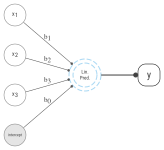
\includegraphics[width=0.5\textwidth,height=\textheight]{index_files/mediabag/img/graphical_lm.pdf}

}

\caption{\label{fig-graph-lm}A linear regression as a graphical model}

\end{figure}%

So at this point you have the basics of what a linear model is and how
it works, and a couple ways to think about it, whether through
programming, math, or just visually. But there is a lot more to it than
that. Just getting the model is easy enough, but we need to be able to
use it and understand the details better, so we'll get into that now!

\section{What do we do with a model?}\label{sec-lm-what-do-we-do}

Once we have a working model, there are two primary ways we can use it.
One way to use a model is to help us understand the relationships
between the features and our outcome of interest. In this way, the focus
can be said to be on \textbf{explanation}, or interpreting the model
results. The other way to use a model is to make estimates about the
outcome for specific observations, often ones we haven't seen in our
data. In this way the focus is on \textbf{prediction}. In practice, we
often do both, but the focus is usually on one or the other. We'll cover
both in detail eventually, but let's start with prediction.

\subsection{Prediction}\label{sec-lm-prediction}

It may not seem like much at first, but a model is of no use if it can't
be used to make predictions about what we can expect in the world around
us. Once our model has been \emph{fit} to the data, we can obtain our
predictions by plugging in values for the features that we are
interested in, and, using the corresponding weights and other parameters
that have been estimated, come to a guess about a specific observation.
Let's go back to our results, starting with a simpler depiction.

\small

\begin{longtable*}{lrrrrrr}
\toprule
feature & estimate & std\_error & statistic & p\_value & conf\_low & conf\_high \\ 
\midrule\addlinespace[2.5pt]
intercept & \textcolor[HTML]{404040}{$3.49$} & \textcolor[HTML]{404040}{$0.04$} & \textcolor[HTML]{404040}{$82.43$} & \textcolor[HTML]{404040}{$0.00$} & \textcolor[HTML]{404040}{$3.41$} & \textcolor[HTML]{404040}{$3.57$} \\ 
word\_count & \textcolor[HTML]{404040}{$-0.04$} & \textcolor[HTML]{404040}{$0.00$} & \textcolor[HTML]{404040}{$-11.58$} & \textcolor[HTML]{404040}{$0.00$} & \textcolor[HTML]{404040}{$-0.05$} & \textcolor[HTML]{404040}{$-0.04$} \\ 
\bottomrule
\end{longtable*}

\normalsize

The table shows the \textbf{coefficient} for each feature including the
intercept, which is our starting point. In this case, the coefficient
for word count is -0.04, which means that for every additional word in
the review, the rating goes down by -0.04 stars. So if we had a review
that was 10 words long, we would \emph{predict} a rating of 3.49 +
10*-0.04 = 3.1 stars.

When we're talking about predictions for a linear model, we usually will
see this as the following mathematically:

\[
\hat{y} = b_0 + b_1x_1 + b_2x_2 + ... + b_nx_n
\]

What is \(\hat{y}\)? The hat over the \(y\) just means that it's a
predicted value of the model, rather than the one we actually observe.
Our first equations that just used \(y\) implicilty suggested that we
would get a perfect rating value given the model, but that's not the
case. We can only get an estimate. The \(\hat{y}\) is also the linear
predictor in our graphical version (Figure~\ref{fig-graph-lm}), which
makes clear it is not the actual target, but a combination of the
features that is related to the target.

To make our first equation accurately reflect the relationship between
the target and our features, we need to add what is usually referred to
as an \textbf{error term}, \(\epsilon\), to account for the fact that
our predictions will not be perfect\footnote{In most circumstances, if
  you ever have perfect prediction, or even near perfect prediction, the
  usual issues are that you have either asked a rather obvious/easy
  question of your data (e.g., predicting whether an image is of a human
  or a car), or have accidentally included the target in your features
  (or a combination of them) in some way.}. So the full linear
(regression) model is:

\[
y = b_0 + b_1x_1 + b_2x_2 + ... + b_nx_n + \epsilon
\]

The error term is a random variable that represents the difference
between the actual value and the predicted value, which comes from the
weighted combination of features. We can't know what the error term is,
but we can estimate it, just like we can the coefficients. We'll talk
more about that in the section on estimation
(Chapter~\ref{sec-estimation}).

TODO: think about which of the following parts of of prediction can move
to the `knowing your model' chap

\subsection{What kinds of predictions can we
get?}\label{sec-lm-prediction-types}

What predictions we get depends on the type of model we are using. For
the linear model, we can get predictions for the target, which is a
\textbf{continuous variable}. Very commonly, we also can get predictions
for a \textbf{categorical target}, such as whether the rating is `good'
or `bad'. This simple breakdown pretty much covers everything, as we
typically would be predicting a continuous variable or a categorical
variable, or more of them, like multiple continuous variables, or a
target with multiple categories, or sequences of categories
(e.g.~words). In our case, we can get predictions for the rating, which
is a number between 1 and 5. Had our target been a binary good vs.~bad
rating, our predictions would still be numeric, and usually expressed as
a probability between 0 and 1, say, for the `good' category. Higher
probabilities would mean we'd more likely predict the movie is good. We
then would convert that probability to a class of good or bad depending
on a chosen probability cutoff. We'll talk about how to get predictions
for categorical targets later.

We previously saw a prediction for a single observation, but we can also
get predictions for multiple observations at once. In fact, we can get
predictions for all observations in our dataset. Besides that, we can
also get predictions for observations that we don't even have data for!
Fun! The following shows how we can get predictions for all data, and
for a single observation with a word count of 5.

\subsubsection{R}

\begin{verbatim}
all_predictions   = predict(model_reviews)

df_prediction = tibble(word_count = 5)
single_prediction = predict(model_reviews, newdata = df_prediction)
\end{verbatim}

\subsubsection{Python}

\begin{verbatim}
all_predictions   = model_reviews.predict()

df_prediction = pd.DataFrame({'word_count': [5]})
single_prediction = model_reviews.predict(df_prediction)
\end{verbatim}

Here is a plot of our predictions for the observed data versus the
actual ratings\footnote{Word count is \textbf{discrete}- it can only
  take whole numbers like 3 or 20, and it is our only feature. Because
  of this, we can only make very limited predicted rating values, while
  the observed rating can take on many other values. Because of this,
  the true plot would show a more banded result with many points
  overlapping, so we use a technique called \textbf{jittering} to move
  the points around a little bit so we can see them all. The points are
  still roughly in the same place, but they are moved around a little
  bit so we can see them all.}. The reference line is where the points
would fall if we had perfect prediction. We can see that the predictions
are definitely not perfect, but we don't expect this. They are not
completely off base either, in that generally higher predicted scores
are associated with higher observed values. We'll talk about how to
assess the quality of our predictions later, but we can at least get a
sense that we have a correspondence relationship between our predictions
and target, which is definitely better than not having a relationship at
all!

\begin{figure}[H]

\centering{

\includegraphics{linear_models_files/figure-pdf/fig-my-first-model-predictions-plot-1.pdf}

}

\caption{\label{fig-my-first-model-predictions-plot}Predictions
vs.~Actual Ratings}

\end{figure}%

Now let's look at what our prediction looks like for a single
observation, and we'll add in a few more- one for 10 words, and one for
a 50 word review, which is beyond the length of any review in this
dataset, and one for 12.3 words, which isn't even possible for this
data, since words are only counted as whole values. To get these values
we just use the same prediction approach we showed above
((\textbf{my-first-model-predictions-r?})), and we specify the word
count value we want to predict for.

\begin{longtable}{rr}

\caption{\label{tbl-predictions}Predictions for Specific Observations}

\tabularnewline

\toprule
Word Count & Predicted Rating \\ 
\midrule\addlinespace[2.5pt]
\textcolor[HTML]{404040}{$5.0$} & \textcolor[HTML]{404040}{$3.3$} \\ 
\textcolor[HTML]{404040}{$10.0$} & \textcolor[HTML]{404040}{$3.1$} \\ 
\textcolor[HTML]{404040}{$12.3$} & \textcolor[HTML]{404040}{$3.0$} \\ 
\textcolor[HTML]{404040}{$50.0$} & \textcolor[HTML]{404040}{$1.4$} \\ 
\bottomrule

\end{longtable}

The values reflect the negative coefficient from our model, reflecting
decreasing ratings with increasing word counts. Furthermore, we see the
power of the model's ability to make predictions for what we don't see
in the data. Maybe we limited our data review size, but we know there
are 50 word reviews out there, and we can still make a guess as to what
the rating would be for such a review. Maybe in another case, we know a
group of people who have on average 12.3 word reviews, and we can make a
guess as to what the average rating would be for that group. Our model
doesn't know anything about the context of the data, but we can use our
knowledge to make predictions about the world around us. This is a very
powerful capability, and it's one of the main reasons we use models in
the first place.

TODO: summarize some thoughts but move bulk to `knowing your model'
chapter

\subsection{Prediction Error}\label{sec-lm-prediction-error}

As we have seen, predictions are not perfect, and an essential part of
the modeling endeavor is to better understand these errors and why they
occur. In addition, error assessment is the fundamental way in which we
assess a model's performance, and, by extension, compare that
performance to other models. In general, prediction error is the
difference between the actual value and the predicted value or some
function of it, and in statistical models, is also often called the
\textbf{residual}. We can look at these individually, or we can look at
them in aggregate with a single metric.

Let's start with looking at the residuals visually. Often the modeling
package you use will have this as a default plotting method when doing a
standard linear regression, so it's wise to take advantage of it. We
plot both the distribution of raw error scores and the cumulative
distribution of absolute prediction error. Here we see a couple things.
First, the distribution is roughly normal, which is a good thing, since
statistical linear regression assumes our error is normally distributed,
and the prediction error serves as an estimate of that. Second, we see
that the mean of the errors is zero, which is a consequence of linear
regression, and the reason we look at other metrics when assessing model
performance. We can also see that most of our predictions are within 1
star rating.

\begin{figure}[H]

\centering{

\includegraphics[width=1\textwidth,height=\textheight]{linear_models_files/figure-pdf/fig-my-first-model-error-plot-1.pdf}

}

\caption{\label{fig-my-first-model-error-plot}Distribution of Prediction
Errors}

\end{figure}%

Of more practical concern is that we don't see extreme values or
clustering, which might indicate a failure on the part of the model to
pick up certain segments of the data. It can still be a good idea to
look at the extremes just in case we can pick up on some aspect of the
data that we could potentially incorporate into the model.

Looking at our worst prediction in absolute terms, we see the
observation has a typical word count, and so our simple model will just
predict a fairly typical rating. But the actual rating is 1, which is
2.1 away from our prediction, a very noticeable difference. Further data
inspection may be required to figure out whiy this came about.

\begin{longtable}{rrr}

\caption{\label{tbl-worst-prediction}Worst Prediction}

\tabularnewline

\toprule
rating & prediction & word\_count \\ 
\midrule\addlinespace[2.5pt]
\textcolor[HTML]{404040}{$1.0$} & \textcolor[HTML]{404040}{$3.1$} & \textcolor[HTML]{404040}{$10$} \\ 
\bottomrule

\end{longtable}

We can also get an overall assessment of the prediction error. In the
case of the linear model we've been looking at, we can express this in a
single metric as the sum or mean of our (squared) errors, the latter of
which is a very commonly used modeling metric- \textbf{MSE} or
\textbf{mean squared error}, or also, its square root - \textbf{RMSE} or
\textbf{root mean squared error}.

If we look back at our results, we can see this expressed as the part of
the output or as an attribute of the model\footnote{The actual divisor
  for linear regression output depends on the complexity of the model,
  and in this case the sum of the squared errors is divided by N-2 (due
  to estimating the intercept and coefficient) instead of N. This is a
  technical detail that would only matter for data too small to make
  much of in the first place, and not important for our purposes here.}.
The RMSE is more interpretable, as it gives us a sense that our typical
errors bounce around by about 0.59. Given that the rating is on a 1-5
scale, this maybe isn't bad, but we could definitely hope to do better
than get within roughly half a point on this scale. We'll talk about
ways to improve this later.

\subsubsection{R}

\begin{verbatim}
summary(model_reviews) # 'Residual standard error' is approx RMSE
\end{verbatim}

\begin{verbatim}

Call:
lm(formula = rating ~ word_count, data = df_reviews)

Residuals:
    Min      1Q  Median      3Q     Max 
-2.0648 -0.3502  0.0206  0.3352  1.8498 

Coefficients:
            Estimate Std. Error t value Pr(>|t|)    
(Intercept)  3.49164    0.04236    82.4   <2e-16 ***
word_count  -0.04268    0.00369   -11.6   <2e-16 ***
---
Signif. codes:  0 '***' 0.001 '**' 0.01 '*' 0.05 '.' 0.1 ' ' 1

Residual standard error: 0.591 on 998 degrees of freedom
Multiple R-squared:  0.118, Adjusted R-squared:  0.118 
F-statistic:  134 on 1 and 998 DF,  p-value: <2e-16
\end{verbatim}

\subsubsection{Python}

\begin{verbatim}
np.sqrt(model_reviews.scale)   # RMSE
\end{verbatim}

\begin{verbatim}
0.590728780660127
\end{verbatim}

At this point you have the gist of prediction and prediction error, but
there is a lot more to it. More detail can be found in the estimation
chapter (Chapter~\ref{sec-estimation}), since we often estimate the
parameters of our model by picking those that will reduce the prediction
error the most. Makes sense right? For now though, let's move on to the
other main use of models, which is to help us understand the
relationships between the features and the target, or
\textbf{explanation}.

TODO: This could possibly be moved to `knowing your model' chapter.
Instead, we could just focus on the coefficient/uncertainty/r2 stuff
here, and then move to the `knowing your model' chapter for the rest. We
could also use other models that would better demonstrate SHAP and other
metrics.

\section{How do we interpret the model?}\label{sec-lm-interpretation}

When it comes to interpreting the results of our model, there are a lot
of tools at our disposal, though many of the tools we can ultimately use
will depend on the specifics of the model we have employed. In general
though, we can group our approach to understanding results at the
\textbf{feature level} and the \textbf{model level}. A feature level
understanding regards the relationship between a single feature and the
target. Beyond that, we also attempt comparisons of feature
contributions to prediction, i.e., relative importance. Model level
interpretation is focused on assessments of how well the model `fits'
the data, or more generally, predictive performance. We'll start with
the feature level, and then move on to the model level.

\subsection{Feature Level}\label{sec-lm-interpretation-feature}

As mentioned, at the feature level, we are primarily concerned with the
relationship between a single feature and the target. More specifically,
we are interested in the direction and magnitude of the relationship,
but in general, it all boils down to how a feature induces change in the
target. For numeric features, we are curious about the change in the
target given some amount of change in the feature values. It's
conceptually the same for categorical features, but often we like to
express the change in terms of group mean differences or something
similar, since the order of categories is not usually meaningful. An
important aspect of feature level interpretation is the specific
predictions we can get by holding the data at key feature values.

\subsubsection{Basics}\label{basics}

Let's start with the basics by looking again at our coefficient table
from the model output.

\small

\begin{longtable*}{lrrrrrr}
\toprule
feature & estimate & std\_error & statistic & p\_value & conf\_low & conf\_high \\ 
\midrule\addlinespace[2.5pt]
intercept & \textcolor[HTML]{404040}{$3.49$} & \textcolor[HTML]{404040}{$0.04$} & \textcolor[HTML]{404040}{$82.43$} & \textcolor[HTML]{404040}{$0.00$} & \textcolor[HTML]{404040}{$3.41$} & \textcolor[HTML]{404040}{$3.57$} \\ 
word\_count & \textcolor[HTML]{404040}{$-0.04$} & \textcolor[HTML]{404040}{$0.00$} & \textcolor[HTML]{404040}{$-11.58$} & \textcolor[HTML]{404040}{$0.00$} & \textcolor[HTML]{404040}{$-0.05$} & \textcolor[HTML]{404040}{$-0.04$} \\ 
\bottomrule
\end{longtable*}

\normalsize

Here, the main thing to look at are the actual feature coefficients and
the direction of their relationship, positive or negative. We saw before
that the coefficient for word count is -0.04, and this means that for
every additional word in the review, the rating goes down by -0.04. So
if we had a review that was 10 words long, we would predict a rating of
3.49 + 10*-0.04 = 3.1 stars.

This interpretation gives us directional information, but how can we
interpret the magnitude of the coefficient? Let's try and use some
context to help us. The value for the coefficient is -0.04, and the
standard deviation of the rating score, i.e., how much it moves around
naturally on its own, is 0.63. So the coefficient is about 6\% of the
standard deviation of the target. In other words, the addition of a
single word to a review results in an expected decrease of 6\% of what
the review would normally bounce around in value. We might not consider
this large, but also, a single word change isn't much. What would be a
significant change in word count? Let's consider the standard deviation
of the feature. In this case, it's 5.07 for word count. So if we
increase the word count by one standard deviation, we expect the rating
to decrease by -0.04 * 5.07 = -0.2. That decrease then translates to a
change of -0.2/0.63 = -0.32 standard deviation units of the target.
Without additional context, many would think that's a significant
change\footnote{Historically, people cite Cohen (2009) for effect size
  guidelines for simple models, but such guidelines are notoriously
  problematic. Rely on your own knowledge of the data, provide reasons
  for your conclusions, and let others draw their own. If you cannot
  tell what would constitute a notable change in your outcome of
  interest, you probably shouldn't be modeling it in the first place.},
or at the very least, that the coefficient is not negligible, and that
the feature is indeed related to the target. But we can also see that
the coefficient is not so large that it's not believable.

\begin{tcolorbox}[enhanced jigsaw, opacityback=0, leftrule=.75mm, bottomrule=.15mm, colframe=quarto-callout-tip-color-frame, rightrule=.15mm, breakable, left=2mm, colback=white, arc=.35mm, toprule=.15mm]

\vspace{-3mm}\textbf{Standardized Coefficients}\vspace{3mm}

The calculation we just did results in what's often called a
`standardized' or `normalized' coefficient. In the case of the simplest
model with only one feature like this, it is identical to the Pearson r
correlation metric, which we invite you to check and confirm on your
own, which should roughly equal our calculation using rounded values. In
the case of multiple features, it represents a (partial) correlation
between the target and the feature, after adjusting for the other
features. But before you start thinking of it as a measure of
\emph{importance}, it is not. It provides some measure of the
feature-target linear relationship, but that doesn't not entail
\emph{practical} importance, nor is it useful in the presence of
nonlinear relationships, interactions, and a host of other interesting
things that are typical to data and models.

\end{tcolorbox}

After assessing the coefficients, next up in our table is the
\textbf{standard error}. The standard error is a measure of how much the
coefficient varies from sample to sample. If we collected the data
multiple times, even under practically identical circumstances, we
wouldn't get the same value each time - it would bounce around a bit,
and the standard error is an estimate of how much it would bounce
around. In other words, the standard error is a measure of
\textbf{uncertainty}, and along with the coefficients, it's used to
calculate everything else in the table. The statistic, here a
t-statistic from the student t distribution\footnote{Most statistical
  tables of this sort will use a t (student t distribution), Z (normal
  distribution), or F (F distribution) statistic. It doesn't really
  matter for your purposes which is used by default, they provide the
  p-value of interest to claim statistical significance.}, is the ratio
of the coefficient to the standard error. This gives us a sense of the
effect relative to its variability, but the statistic's primary use is
to calculate the \textbf{p-value} related to its
distribution\footnote{You can calculate this as
  \texttt{pt(stat,\ df\ =\ model\ degrees\ of\ freedom,\ lower=FALSE)*2}
  in R or \texttt{stats.t.cdf} in Python. The model degrees of freedom
  are provided in the summary output (a.k.a. residual degrees of
  freedom) \texttt{lower=FALSE} and \texttt{*2} are to get the two-sided
  p-value, which is what we want in this case. When it comes to t and Z
  statistics, anything over 2 is statistically significant by the common
  standard of a p-value of .05 or less. Note also that even though
  output will round it to zero, the true p-value can never be zero.},
which is the probability of seeing a coefficient as large as the one we
have, \emph{if} we assume from the outset that the true value of the
coefficient is zero. In this case, the p-value is 3.47e-29, which is
very small. We can conclude that the coefficient is statistically
different from zero, and that the feature is related to the target, at
least statistically speaking. However, the interpretation we used
regarding the coefficient previously is far more useful than the
p-value, as the p-value can be affected by many things not necessarily
related to the feature-target relationship, such as sample size, and is
often misinterpreted.

Aside from the coefficients, the most important output is the
\textbf{confidence interval} (CI). The CI is a range of values that
encapsulates the uncertainty we have in our guess about the
coefficients. While our best guess for the effect of word count on
rating is -0.04, we know it's not \emph{exactly} that, and the CI gives
us a range of reasonable values we might expect the effect to be based
on the data at hand and the model we've employed. In this case, the
default is a 95\% confidence interval, and we can think of this
particular confidence interval like
\href{https://en.wikipedia.org/wiki/Horseshoes_(game)}{throwing
horseshoes}. If we kept collecting data and running models, 95\% of our
CIs would capture the true value, and this is one of the many possibile
CIs we could have gotten. That's the technical definition, which is a
bit abstract\footnote{The interpretation regarding the CI is even more
  nuanced than this, but we'll leave that for another time. For now,
  we'll just say that the CI is a range of values that are good guesses
  for the true value. Your authors have used frequentist and Bayesian
  statistics for many years, and we are fine with both of them, because
  they both work well enough in the real world. Despite where this
  ranged estimate comes from, the vast majority use CIs in the same way,
  and they are a useful tool for understanding the uncertainty in our
  estimates.}, but we can also think of it more simply as a range of
values that are good guesses for the true value. In this case, the CI is
-0.05 to -0.035, and we can be 95\% confident that a good range for the
coefficient is between those values. We can also see that the CI is
relatively narrow, which is good, as it implies that we have a good idea
of what the coefficient is. If it was very wide, we would have a lot of
uncertainty about the coefficient, and we would not likely not want to
base important decisions regarding it.

\includegraphics[width=0.5\textwidth,height=\textheight]{img/horseshoes.jpeg}

Keep in mind that your model has a lot to say about what you'll be able
to say at the feature level. As an example, as we get into machine
learning models, you won't have as easy a time with coefficients and
their confidence intervals. For now we'll stop here, but there is a lot
more to the story when it comes to feature level interpretation, and
we'll continue to return to the topic. But first, let's take a look at
interpreting things in another way.

\begin{tcolorbox}[enhanced jigsaw, opacityback=0, leftrule=.75mm, bottomrule=.15mm, colframe=quarto-callout-tip-color-frame, rightrule=.15mm, breakable, left=2mm, colback=white, arc=.35mm, toprule=.15mm]

\vspace{-3mm}\textbf{Hypothesis Testing}\vspace{3mm}

The confidence interval and p-value will for coefficients in typical
statistical linear models will coincide with one another in that, if for
a given alpha signficance level, if a 1-alpha\% CI includes zero, then
your p-value will be greater than alpha, and vice versa. This is because
the same standard error is used to calculate both. However, the
framework of using a CI vs.~using the p-value for claiming statistical
significance actually came from individuals that were philosophically
opposed. Modern day usage of both is a bit of a mess that would upset
both Fisher (p-value guy) and Neyman (CI guy), but your authors find
that this incorrect practical usage doesn't make much practical
difference in the end.

\end{tcolorbox}

\subsection{Is it a Good Model?}\label{sec-lm-interpretation-model}

Thus far, we've focused on interpretation at the feature level. But
knowing the interpretation of a feature doesn't do you much good if the
model itself is poor! In that case, we also need to assess the model as
a whole, and as with the feature level, we can go about this in a few
ways. Before getting too carried away with asking whether your model is
any good or not, you always need to ask your self \emph{relative to
what}? Many models claim top performance under various circumstances,
but which are statistically indistinguishable from many other models. So
we need to be careful about how we assess our model, and what we compare
it to.

First, we can start with the predictions of our model. As noted
previously, how well the predictions and target line up is a measure of
how well the model fits the data. Most model-level interpretation
involves assessing and comparing model fit and variations on this theme.
One of the better ways to assess model fit is visually, so let's look at
our predictions vs.~the target.

\subsubsection{R}

\begin{verbatim}
predictions = predict(model_reviews)
y = df_reviews$rating
\end{verbatim}

\subsubsection{Python}

\begin{verbatim}
predictions = model_reviews.predict()
y = df_reviews.rating
\end{verbatim}

\begin{figure}[H]

\centering{

\includegraphics{linear_models_files/figure-pdf/fig-pp-scatter-1.pdf}

}

\caption{\label{fig-pp-scatter}Predictions vs.~Observed Ratings}

\end{figure}%

The one on the left is using the raw target and predictions, and they
appear very grid-like. The reason is that our ratings are only at the
single decimal place precision, and our word count is at the integer
level precision, so we have a lot of ties. The right side jitters the
data randomly a bit so we can see a better pattern, but is otherwise the
same. In general, the closer to a line this plot becomes the better, so
we can tell already there is still a lot of noise left to explain beyond
our model.

\subsubsection{Model Metrics}\label{sec-lm-interpretation-model-metrics}

We've already discussed mean-squared error\footnote{Any time we're
  talking about MSE, we're also talking about RMSE as it's just the
  square root of MSE, so which you choose is mostly arbitrary.}, but
there are other metrics we can use to assess \textbf{model fit}. As we
noted, (R)MSE is a very popular measure for continuous targets, telling
us the standard deviation of errors, or how much they bounce around on
average. In our case, the value was 0.59. Another metric we can use in
this particular situation is the mean absolute error, which is similar
to the mean squared error, but instead of squaring the errors, we just
take the absolute value. Conceptually it attempts to get at the same
idea, how much our predictions miss on average, and here the value is
0.46, which we actually showed in our initial residual plot
(Figure~\ref{fig-my-first-model-error-plot}). With either metric, the
closer to zero the better, since as we get closer, we are reducing
error.

We can also look at the \textbf{R-squared} (R\textsuperscript{2}) value
of the model. R\textsuperscript{2} is possibly the most popular measure
of model performance with linear regression and linear models in
general. Before squaring, it's just the correlation of the values that
we saw in the previous plot (Figure~\ref{fig-pp-scatter}). When we
square it, we can interpret it as a measure of how much of the variance
in the target is explained by the model. In this case, our model shows
the R\textsuperscript{2} is 0.12, which is not bad for a single feature
model in this type of setting. We interpret it that 12\% of the target
is explained by our model. In addition, we can also interpret
R\textsuperscript{2} as 1 - the prorportion of error varaince in the
target, which we can calculate as \(1 - \frac{\textrm{MSE}}{var(y)}\).
In other words the complement of R\textsuperscript{2} is the proportion
of the variance in the target that is not explained by the model. Either
way, since -11\% is not explained by the model, our result suggests
there is plenty of work left to do!

Note also, that with R\textsuperscript{2} we get a sense of the variance
shared between \emph{all} features in the model and the target, however
complex the model gets. As long as we use it descriptively as a simple
correspondence assessment of our predictions and target, it's a fine
metric. For various reasons, it's not a great metric for comparing
models to each other, but again, as long as you don't get carried away,
it's okay to use.

\subsection{Prediction
vs.~Explanation}\label{sec-lm-prediction-vs-explanation}

In your humble authors' views, one can't stress enough the importance of
a model's ability to predict the target. It can be a poor model, maybe
because the data is not great, or perhaps we're exploring a new area of
research, but we'll always be interested in how well a model
\textbf{fits} the observed data, and predicts new data.

Even to this day, \textbf{statistical significance} is focused on a
great deal, even to the point that a much hullabaloo is made about
models that have no predictive power at all. As strange as it may sound,
you can read whole journal articles, news features, and business reports
in many fields with hardly any mention of prediction. The focus is
almost entirely on the \textbf{explanation} of the model, and usually
the statistical significance of the features. In those settings,
statistical significance is often used as a proxy for importance, which
it never should be. Unfortunately, statistical significance is affected
by other things besides the size of the coefficient, and without an
understanding of the context of the features, in this case, like how
long typical reviews are, what their range is, what variability of
ratings is, etc., the information it provides is extremely limited, and
many would argue, not even useful at all. If we are very interested in
the coefficient or weight value specifically, it is better to focus on
the range of possible values, which is provided by the confidence
interval. While a confidence interval is also a loaded description of a
feature's relationship to the target, we can use it in a very practical
way as a range of possible values for that weight, and more importantly,
\emph{think of possibilities rather than certainties}.

Suffice it to say at this point that how much one focuses on prediction
vs.~explanation depends on the context and goals of the data endeavor.
There are cases where predictive capability is of utmost importance, and
we care less about about explanatory details, but not to the point of
ignoring it. For example, even with deep learning models for image
classification, where the inputs are just RGB values, we'd still like to
know what the (notably complex) model is picking up on, otherwise we may
be classifying images based on something like image backgrounds
(e.g.~outdoors vs.~indoors) instead of the objects of actual interest
(dogs vs.~cats). In some business or other organizational settings, we
are very or even mostly interested in the coefficients/weights, which
might indicate how to allocate monetary resources in some fashion. But
if those weights come from a model with no predictive power, placing
much importance on them may be a fruitless endeavor.

In the end we'll need to balance our efforts to suit the task at hand.
Prediction and explanation are both fundamental to the modeling
endeavor.

\section{Adding Complexity}\label{sec-lm-complexity}

We've seen how to fit a model with a single feature and interpret the
results, and that helps us to get oriented to the process. However,
we'll always have more than one feature for a model except under some
very specific circumstances, such as exploratory data analysis. So let's
see how we can do that with a model that makes more sense.

\subsection{Multiple Features}\label{sec-lm-multiple-features}

We can add more features to our model very simply. Using the standard
functions we've already demonstrated, we just add them to the formula
(both R and statsmodels) as follows.

\begin{verbatim}
'y ~ feature_1 + feature_2 + feature_3'
\end{verbatim}

In other cases where we use matrix inputs, additional features will just
be the additional input columns, and nothing about the model code
actually changes. We might have a lot of features, and even for
relatively simple linear models this could be dozens in some scenarios.
A compact depiction of our model uses the matrix representation, which
we'll show in the callout below, and you can find more detail in the
matrix section Appendix~\ref{sec-matrix-operations} overview. For our
purposes, all you really need to know is that this:

\begin{equation}\phantomsection\label{eq-lm-XB}{
y = X\beta\qquad  \textrm{or}\qquad y = \alpha + X\beta
}\end{equation}

is the same as this:

\[
y = \alpha + \beta_1 x_1 + \beta_2 x_2 + \beta_3 x_3 \dots
\]

where \(X\) is a matrix of features\footnote{In the first depiction
  without \(\alpha\), there is an additional column at the beginning of
  the matrix that is all ones, which is a way to incorporate the
  intercept into the model. However, most models that use a matrix as
  input will not have the intercept column, as it's not part of the
  model estimation or is estimated separately.}, and \(\beta\) is a
vector of coefficients. Matrix multiplication provides us an efficient
way to get our expected value/prediction.

\begin{tcolorbox}[enhanced jigsaw, opacityback=0, leftrule=.75mm, bottomrule=.15mm, colframe=quarto-callout-note-color-frame, rightrule=.15mm, breakable, left=2mm, colback=white, arc=.35mm, toprule=.15mm]

\vspace{-3mm}\textbf{Matrix Representation of a Linear Model}\vspace{3mm}

Here we'll show the matrix representation form of the linear model in
more detail. In the following, \(y\) is a vector of all target
observations, and \(X\) is a matrix of features. The \(\beta\) vector is
the vector of coefficients. The column of 1s serves as a means to
incorporate the intercept, as it's just mulitplied by whatever the
estimated intercept value is. The matrix multiplication form is just a
compact way of expressing the sum of the features multiplied by their
coefficients.

Here is y as a vector of observations, n x 1.

\begin{equation}\phantomsection\label{eq-lm-mat-y}{
\textbf{y} = \begin{bmatrix}
y_1 \\
y_2 \\
\vdots \\
y_n
\end{bmatrix}
}\end{equation}

Here is the n x p matrix of features, including the intercept:

\begin{equation}\phantomsection\label{eq-lm-mat-x}{
\textbf{X} = \begin{bmatrix}
1 & x_{11} & x_{12} & \dots & x_{1p} \\
1 & x_{21} & x_{22} & \dots & x_{2p} \\
\vdots & \vdots & \vdots & \ddots & \vdots \\
1 & x_{n1} & x_{n2} & \dots & x_{np}
\end{bmatrix}
}\end{equation}

And finally, here is the p x 1 vector of coefficients:

\begin{equation}\phantomsection\label{eq-lm-mat-b}{
\bf{\beta} = \begin{bmatrix}
b_0 \\
b_1 \\
\vdots \\
b_p
\end{bmatrix}
}\end{equation}

Putting it all together, we get the linear model in matrix form:

\begin{equation}\phantomsection\label{eq-lm-mat-mult}{
\bf{y = X\beta }
}\end{equation}

You will also see it depicted in a transposed fashion, such that
\(y = \beta X\), which is just a matter of preference, except that it
assumes your data is formatted where the features are the rows and the
observations are the columns. You'll rarely if ever see data stored this
way in practice for tabular data, but you should be aware that other
data settings will force you to think of multi-dimensional
arrays\footnotemark{} instead of 2-d matrices, for example, with image
processing. So it's good to be flexible.

\end{tcolorbox}

\footnotetext{In deep learning, models arrays are referred to as the
more abstract representation of \textbf{tensors}, but for practical
purposes the distinction doesn't really matter for modeling, as the
tensors are always represented as some n-dimensional array.}

With that in mind, let's get to our model! In what follows, we keep the
word count, but now we add some aspects of the reviewer, such as age and
the number of children in the household, and features related to the
movie, like the release year, the length of the movie in minutes, and
the total reviews received. We'll also add another review level feature-
the year the review was written. We'll use the same approach as before,
and literally just add them as we depicted in our linear model formula
(Equation~\ref{eq-lm-basic}).

\subsubsection{R}

\begin{verbatim}
model_reviews_extra = lm(
    rating ~
        word_count
        + age
        + review_year
        + release_year
        + length_minutes
        + children_in_home
        + total_reviews,
    data = df_reviews
)

summary(model_reviews_extra)
\end{verbatim}

\begin{verbatim}

Call:
lm(formula = rating ~ word_count + age + review_year + release_year + 
    length_minutes + children_in_home + total_reviews, data = df_reviews)

Residuals:
    Min      1Q  Median      3Q     Max 
-1.8231 -0.3399  0.0107  0.3566  1.5144 

Coefficients:
                  Estimate Std. Error t value Pr(>|t|)    
(Intercept)      -4.56e+01   7.46e+00   -6.11  1.5e-09 ***
word_count       -3.03e-02   3.33e-03   -9.10  < 2e-16 ***
age              -1.69e-03   9.24e-04   -1.83   0.0683 .  
review_year       9.88e-03   3.23e-03    3.05   0.0023 ** 
release_year      1.33e-02   1.79e-03    7.43  2.3e-13 ***
length_minutes    1.67e-02   1.53e-03   10.90  < 2e-16 ***
children_in_home  1.03e-01   2.54e-02    4.05  5.5e-05 ***
total_reviews     7.62e-05   6.16e-06   12.36  < 2e-16 ***
---
Signif. codes:  0 '***' 0.001 '**' 0.01 '*' 0.05 '.' 0.1 ' ' 1

Residual standard error: 0.52 on 992 degrees of freedom
Multiple R-squared:  0.321, Adjusted R-squared:  0.316 
F-statistic:   67 on 7 and 992 DF,  p-value: <2e-16
\end{verbatim}

\subsubsection{Python}

\begin{verbatim}
model_reviews_extra = smf.ols(
    formula = 'rating ~ word_count \
        + age \
        + review_year \
        + release_year \
        + length_minutes \
        + children_in_home \
        + total_reviews',
    data = df_reviews
).fit()

model_reviews_extra.summary(slim = True)
\end{verbatim}

\begin{verbatim}
<class 'statsmodels.iolib.summary.Summary'>
"""
                            OLS Regression Results                            
==============================================================================
Dep. Variable:                 rating   R-squared:                       0.321
Model:                            OLS   Adj. R-squared:                  0.316
No. Observations:                1000   F-statistic:                     67.02
Covariance Type:            nonrobust   Prob (F-statistic):           3.73e-79
====================================================================================
                       coef    std err          t      P>|t|      [0.025      0.975]
------------------------------------------------------------------------------------
Intercept          -45.5688      7.463     -6.106      0.000     -60.215     -30.923
word_count          -0.0303      0.003     -9.102      0.000      -0.037      -0.024
age                 -0.0017      0.001     -1.825      0.068      -0.004       0.000
review_year          0.0099      0.003      3.055      0.002       0.004       0.016
release_year         0.0133      0.002      7.434      0.000       0.010       0.017
length_minutes       0.0167      0.002     10.897      0.000       0.014       0.020
children_in_home     0.1028      0.025      4.051      0.000       0.053       0.153
total_reviews     7.616e-05   6.16e-06     12.362      0.000    6.41e-05    8.83e-05
====================================================================================

Notes:
[1] Standard Errors assume that the covariance matrix of the errors is correctly specified.
[2] The condition number is large, 2.82e+06. This might indicate that there are
strong multicollinearity or other numerical problems.
"""
\end{verbatim}

There is definitely more to unpack here, but it's important to note that
it's just \emph{more} stuff, not \emph{different} stuff. The model-level
components are the same in that we still see R\textsuperscript{2} etc.,
although they are all `better' (higher R\textsuperscript{2}, lower
error) because we have a more predictive model. Our coefficents look the
same also, and we'd interpret the in the same way. Starting with word
count, we see that it's still statistically significant, but it has been
reduced just slightly from our previous model where it was the only
feature (-0.04 vs.~-0.03). Why? This suggests that word count has some
non-zero correlation, sometimes called \textbf{collinearity}, with other
features that are also explaining the target to some extent. Our linear
model shows the effect of each feature \emph{controlling for other
features}, or, \emph{holding other features constant}\footnote{A lot of
  statisticians and causal modeling folks get very hung up on the
  terminology here, but we'll leave that to them as we'd like to get on
  with things. For our purposes, we'll just say that we're interested in
  the effect of a feature \emph{after} we've accounted for the other
  features in the model.}. Conceptually this means that the effect of
word count is the effect of word count \emph{after} we've accounted for
the other features in the model. In this case, an increase of a single
word results in a -0.03 drop, even after adjusting for the effect of
other features. Looking at another feature, the addition of a child to
the home is associated with 0.1 bump in rating, accounting for the other
features.

Thinking about prediction, how would we get a prediction for a movie
rating with a review that is 12 words long, written in 2020, by a 30
year old with one child, for a movie that is 100 minutes long, released
in 2015, with 10000 total reviews? Exactly the same as we did before
(Section~\ref{sec-lm-prediction-types})! We just create a data frame
with the values we want, and predict accordingly.

\subsubsection{R}

\begin{verbatim}
predict_observation = tibble(
    word_count = 12,
    age = 30,
    children_in_home = 1,
    review_year = 2020,
    release_year = 2015,
    length_minutes = 100,
    total_reviews = 10000
)

predict(
    model_reviews_extra,
    newdata = predict_observation
)
\end{verbatim}

\begin{verbatim}
   1 
3.26 
\end{verbatim}

\subsubsection{Python}

\begin{verbatim}
predict_observation = pd.DataFrame(
    {
        'word_count': 12,
        'age': 30,
        'children_in_home': 1,
        'review_year': 2020,
        'release_year': 2015,
        'length_minutes': 100,
        'total_reviews': 10000
    },
    index = ['new_observation']
)

model_reviews_extra.predict(predict_observation)
\end{verbatim}

\begin{verbatim}
new_observation    3.2595
dtype: float64
\end{verbatim}

In our example we're just getting a single prediction, but don't let
that hold you back! You can predict an entire data set if you want, and
use any values for the features you want. We'll do this explicitly later
on, but for now, try getting a prediction for a different set of values.

TODO: Reconcile with Data chapter, possibly remove from this chapter
entirely. If we do, maybe add this model example to that chapter.

\subsection{Categorical Features}\label{sec-lm-categorical-features}

Categorical features can be added to a model just like any other
feature. The main issue is that they have to be represented numerically,
because models only work on numerically coded features and targets. The
simplest and most common encoding is called a \textbf{one-hot encoding}
scheme, which creates a new feature for each category, and assigns a 1
if the observation is in that category, and a 0 otherwise. This is also
called a \textbf{dummy coding} when used for statistical models. Here is
an example of what the coding looks like for the season feature. This is
really all there is to it.

\begin{longtable*}{rlrrrr}
\toprule
rating & season & Fall & Summer & Winter & Spring \\ 
\midrule\addlinespace[2.5pt]
\textcolor[HTML]{404040}{$2.70$} & Fall & \textcolor[HTML]{404040}{$1$} & \textcolor[HTML]{404040}{$0$} & \textcolor[HTML]{404040}{$0$} & \textcolor[HTML]{404040}{$0$} \\ 
\textcolor[HTML]{404040}{$4.20$} & Fall & \textcolor[HTML]{404040}{$1$} & \textcolor[HTML]{404040}{$0$} & \textcolor[HTML]{404040}{$0$} & \textcolor[HTML]{404040}{$0$} \\ 
\textcolor[HTML]{404040}{$3.70$} & Fall & \textcolor[HTML]{404040}{$1$} & \textcolor[HTML]{404040}{$0$} & \textcolor[HTML]{404040}{$0$} & \textcolor[HTML]{404040}{$0$} \\ 
\textcolor[HTML]{404040}{$2.70$} & Fall & \textcolor[HTML]{404040}{$1$} & \textcolor[HTML]{404040}{$0$} & \textcolor[HTML]{404040}{$0$} & \textcolor[HTML]{404040}{$0$} \\ 
\textcolor[HTML]{404040}{$2.40$} & Summer & \textcolor[HTML]{404040}{$0$} & \textcolor[HTML]{404040}{$1$} & \textcolor[HTML]{404040}{$0$} & \textcolor[HTML]{404040}{$0$} \\ 
\textcolor[HTML]{404040}{$4.00$} & Summer & \textcolor[HTML]{404040}{$0$} & \textcolor[HTML]{404040}{$1$} & \textcolor[HTML]{404040}{$0$} & \textcolor[HTML]{404040}{$0$} \\ 
\textcolor[HTML]{404040}{$1.80$} & Fall & \textcolor[HTML]{404040}{$1$} & \textcolor[HTML]{404040}{$0$} & \textcolor[HTML]{404040}{$0$} & \textcolor[HTML]{404040}{$0$} \\ 
\textcolor[HTML]{404040}{$2.40$} & Summer & \textcolor[HTML]{404040}{$0$} & \textcolor[HTML]{404040}{$1$} & \textcolor[HTML]{404040}{$0$} & \textcolor[HTML]{404040}{$0$} \\ 
\textcolor[HTML]{404040}{$2.50$} & Winter & \textcolor[HTML]{404040}{$0$} & \textcolor[HTML]{404040}{$0$} & \textcolor[HTML]{404040}{$1$} & \textcolor[HTML]{404040}{$0$} \\ 
\textcolor[HTML]{404040}{$4.30$} & Summer & \textcolor[HTML]{404040}{$0$} & \textcolor[HTML]{404040}{$1$} & \textcolor[HTML]{404040}{$0$} & \textcolor[HTML]{404040}{$0$} \\ 
\bottomrule
\end{longtable*}

When using statistical models we don't have to do this ourselves. Even
other tools for machine learning models will typically have a way to
identify and appropriately handle categorical features, even in very
complex ways when it comes to deep learning models. What is important is
to be aware that they require special handling, but often this is done
behind the scenes. Now let's do a quick example using a categorical
feature with our data, and we'll keep a numeric feature as well just for
consistency.

\subsubsection{R}

\begin{verbatim}
model_cat = lm(
    rating ~ word_count + season,
    data = df_reviews
)

summary(model_cat)
\end{verbatim}

\begin{verbatim}

Call:
lm(formula = rating ~ word_count + season, data = df_reviews)

Residuals:
    Min      1Q  Median      3Q     Max 
-1.9184 -0.3622  0.0133  0.3589  1.8372 

Coefficients:
             Estimate Std. Error t value Pr(>|t|)    
(Intercept)    3.3429     0.0530   63.11  < 2e-16 ***
word_count    -0.0394     0.0036  -10.96  < 2e-16 ***
seasonSpring  -0.0301     0.0622   -0.48     0.63    
seasonSummer   0.2743     0.0445    6.17  9.8e-10 ***
seasonWinter  -0.0700     0.0595   -1.18     0.24    
---
Signif. codes:  0 '***' 0.001 '**' 0.01 '*' 0.05 '.' 0.1 ' ' 1

Residual standard error: 0.572 on 995 degrees of freedom
Multiple R-squared:  0.176, Adjusted R-squared:  0.173 
F-statistic: 53.1 on 4 and 995 DF,  p-value: <2e-16
\end{verbatim}

\subsubsection{Python}

\begin{verbatim}
model_cat = smf.ols(
    formula = "rating ~ word_count + season",
    data = df_reviews
).fit()

model_cat.summary(slim = True)
\end{verbatim}

\begin{verbatim}
<class 'statsmodels.iolib.summary.Summary'>
"""
                            OLS Regression Results                            
==============================================================================
Dep. Variable:                 rating   R-squared:                       0.176
Model:                            OLS   Adj. R-squared:                  0.173
No. Observations:                1000   F-statistic:                     53.09
Covariance Type:            nonrobust   Prob (F-statistic):           1.41e-40
====================================================================================
                       coef    std err          t      P>|t|      [0.025      0.975]
------------------------------------------------------------------------------------
Intercept            3.3429      0.053     63.109      0.000       3.239       3.447
season[T.Spring]    -0.0301      0.062     -0.483      0.629      -0.152       0.092
season[T.Summer]     0.2743      0.044      6.171      0.000       0.187       0.362
season[T.Winter]    -0.0700      0.059     -1.177      0.239      -0.187       0.047
word_count          -0.0394      0.004    -10.963      0.000      -0.047      -0.032
====================================================================================

Notes:
[1] Standard Errors assume that the covariance matrix of the errors is correctly specified.
"""
\end{verbatim}

We now see the usual output. There is word count again, with its
slightly negative assocation with rating. And we have an effect for each
season as well\ldots{} except, wait a second, where is the fall effect?
The coefficients are interepreted the same way - as we move one unit on
x, we see a corresponding change in y. But moving from one category to
another requires starting at some category in the first place! So one is
chosen arbitrarily, but you would have control over this. In our model,
fall is chosen because its first alphabetically. So if we look at say,
the effect of summer, we see an increase in the rating of 0.27 relative
to fall.

A better approach to understanding categorical features for standard
linear models is through what are called \textbf{marginal effects},
which can provide a kind of average prediction for each category while
accounting for the other features in the model. Better still is to
visualize these, and we can use something like our PDP approach from
before to do so\footnote{At the time of this writing, there seems to be
  very little for this sort of thing in Python. statsmodels provides
  limited functionality, but only for logistic regression models. In R
  you have various tools like \texttt{marginaleffects},
  \texttt{emmeans}, \texttt{ggeffects} and more.}. It's actually tricky
to define `average' when there are multiple features and interactions
involved, so be careful, but we'd interpret the result similarly in
those cases as best we can. In this case, we expect higher ratings for
summer releases.

\begin{figure}[H]

{\centering \includegraphics{linear_models_files/figure-pdf/cat-feature-viz-r-1.pdf}

}

\caption{Marginal Effects of Season on Rating}

\end{figure}%

\subsection{Other Complexity}\label{sec-lm-other-complexity}

\section{Assumptions and More}\label{sec-lm-assumptions}

TODO: MOVE BULK OF THIS TO MODEL CRITICISM?? ALSO NEEDS CLEANUP

Every model you use has underlying assumptions which, if not met, could
potentially result in incorrect inferences about the effects,
performance, or predictive capabilities of the model. The standard
linear regression model we've shown is no different, and it has a number
of assumptions that must be met for it to be \emph{statistically} valid.
Briefly they are:

\begin{itemize}
\tightlist
\item
  That your model is not grossly misspecified (e.g., you've included the
  right features and not left out important ones)
\item
  The data that you're modeling reflects the population you want to make
  generalizations about
\item
  The model is linear in the parameters (i.e.~no \(\beta_1\cdot e^x\)
  type stuff)
\item
  The features are not correlated with the error (prediction errors,
  unobserved causes)
\item
  Your data observations are independent of each other
\item
  The prediction errors are homoscedastic (don't have large errors with
  certain predictions vs low with others)
\item
  Normality of the errors (i.e.~your prediction errors). Another way to
  put it is that your target variable is normally distributed
  conditional on the features.
\end{itemize}

Things a linear regression model does not assume:

\begin{itemize}
\tightlist
\item
  That the features are normally distributed

  \begin{itemize}
  \tightlist
  \item
    For example, using categorical features is fine
  \end{itemize}
\item
  That the relationship between the features and target is linear

  \begin{itemize}
  \tightlist
  \item
    Interactions, polynomial terms, etc. are all fine
  \end{itemize}
\item
  That the features are not correlated with each other

  \begin{itemize}
  \tightlist
  \item
    They usually are
  \end{itemize}
\end{itemize}

If you do meet these assumptions, it doesn't mean:

\begin{itemize}
\tightlist
\item
  You have large effects
\item
  You have a good model
\item
  You have causal effects
\item
  You (necessarily) have less uncertainty about your coefficients or
  predictions than other methods
\end{itemize}

If you don't meet these assumptions, it doesn't mean:

\begin{itemize}
\tightlist
\item
  That your model will have poor predictions
\item
  That your conclusions will necessarily be incorrect
\end{itemize}

So basically whether or not you meet the assumptions of your model
doesn't actually say much about whether the model is great or terrible,
it just means that you have to be careful about what you can say about
it. For the linear regression model, if you do meet those assumptions,
your coefficient estimates are unbiased\footnote{This means they are
  correct on average, not the true value. And if they were biased, this
  is statistical bias, and has nothing to do with the moral or ethical
  implications of the data, or whether the features themselves are
  biased in measurement. Culturally biased data is a different problem
  than statistical/prediction bias or measurement error, though they are
  not mutually exclusive. The latter can more readily be tested, while
  the former is usually more difficult to assess. For example, if our
  movie reviews only came from a website with a paywall, they would be
  biased if we wanted to use them to refer to general public opinion.
  Even then, our model results are perfectly reasonable, as long as they
  are used to generalize only to that population of people who pay for
  the website. If we wanted to generalize to the general public, we
  would need to account for this bias in some way, or use a different
  data source. MOVE THIS TO SOME OTHER CHAPTER (DATA?)}, and in general,
your statistical inferences are correct ones. If you don't meet them,
there are alternative versions of the linear model you could use that
would get around the problem. For example, data that runs over a
sequence of time (\textbf{time series} data) violates the independence
assumption since observations closer in time are more likely to be
similar than those farther apart. But we would use a \textbf{time
series} or similar model instead to account for this. If normality is
difficult to meet, you could assume a different data generating
distribution. We'll discuss some of these in
Chapter~\ref{sec-lm-extend}, but it's also important to note that not
meeting the assumptions may only mean you'll prefer a different type of
linear or other model to use for the data. It's often the case taht not
meeting the assumptions is often the result of a poor model, e.g., using
poor features in an \textbf{underspecified} way, like not including
interactions or other complexity.

On top of not meeting the assumptions, we may in fact intentionally
introduce bias to get better prediction! For example, we might use a
\textbf{penalized regression} model to reduce the variance in our
predictions, at the cost of introducing bias in the coefficients. We'll
talk more of this in the Chapter~\ref{sec-ml-common-models}, but suffice
it to say for now, if you are more interested in prediction, you may be
less interested in the statistical assumptions of the basic linear
model.

\subsection{More Complex Models}\label{sec-lm-more-complex}

Let's say your running some XGBoost or Deep Linear Model and getting
outstanding predictions. Assumptions smumptions you say! And you might
even be right! But if you want to talk confidently about feature
contributions, or know something about the uncertainty in the
predictions (which you're assessing right?), well, maybe you might want
to know if you're meeting your assumptions. Some of them are:

\begin{itemize}
\tightlist
\item
  You have enough data to make the model generalizable
\item
  Your data isn't biased (e.g., you don't have 90\% of your data from
  one region when you want to talk about a whole area)
\item
  You adequately sampled the hyperparameter space (e.g.~you didn't just
  use the defaults or a small grid search)
\item
  Your observations are independent or at least \textbf{exchangeable}
  and don't have \textbf{data leakage}, or you are explicitly modeling
  observation dependence
\item
  That all the parameter settings you set are correct or at least viable
  (e.g.~you let the model run for a long enough set of iterations, your
  batch size was adequate, you had enough hidden layers, etc.)
\end{itemize}

And if you want to talk about specific feature contributions, you are
assuming:

\begin{itemize}
\tightlist
\item
  The features are largely uncorrelated
\item
  The features largely do not interact (but then why are you doing a
  complex model that is inherently interactive), or that your
  understanding of feature contribution deals with the interactions
\end{itemize}

Yeah\ldots{} so, sorry to say, using non-statistical models doesn't mean
you don't have to worry about assumptions, you still have some of the
old stuff and some new ones to boot.

\section{Classification}\label{sec-lm-classification}

We've been using a continuous target, but what about a categorical
target? For example, what if we just had a binary target of whether a
movie was good or bad? We will dive much more into classification models
in our upcoming chapters, but it turns out that we can still formulate
it as a linear model problem. The main difference is that we use a
transformation of our linear combination of features, using what is
sometimes called a \textbf{link function}, and we'll need to use a
different \textbf{objective function} rather than least squares, such as
the binomial likelihood, to deal with the binary target. This also means
we'll move away from R\textsuperscript{2} as a measure of model fit, and
look at something something else, like accuracy.

Graphically we can see it in the following way, which when compared with
our linear model (Figure~\ref{fig-graph-lm}), doesn't look much
different. In what follows, we create our linear combination and put it
through the sigmoid function, which is a common link function for binary
targets\footnote{The sigmoid function in this case is the inverse
  logistic function, and the resulting statistical model is called
  logistic regression. In other contexts the model would not be a
  logistic regression, but this is still a very commmonly used
  \emph{activation function}. But many others could potentially be used
  e.g.~using a normal instead of logistic distribution, resulting in the
  so-called probit model.}. The result is a probability, which we can
then use to classify the observation as good or bad based on a chosen
threshold.

\begin{figure}[H]

\centering{

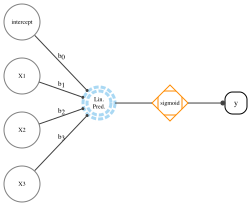
\includegraphics[width=0.75\textwidth,height=\textheight]{index_files/mediabag/img/graphical_logistic.pdf}

}

\caption{\label{fig-graph-logistic}A Linear Model with Transformation
Can Be a Logistic Regression}

\end{figure}%

As soon as we move away from the standard linear model and use
transformations of our linear predictor, simple coefficient
interpretation becomes difficult, sometimes exceedingly so. We will
explore more of these types of models in Chapter~\ref{sec-glm}.

\section{More linear models}\label{sec-lm-more}

Before we leave our humble linear model, let's look at some others. Here
is a brief overview of some of the more common linear models you might
encounter.

Generalize Linear Models and related

\begin{itemize}
\tightlist
\item
  True GLM e.g.~logistic, poisson
\item
  Other distributions: beta regression, tweedie, t (so-called robust),
  truncated
\item
  Penalized regression: ridge, lasso, elastic net
\item
  Censored outcomes: Survival models, tobit
\end{itemize}

Multivariate/multiclass/multipart

\begin{itemize}
\tightlist
\item
  Multivariate regression (multiple targets)
\item
  Multinomial/Categorical/Ordinal regression (\textgreater2 classes)
\item
  Zero (or some number) -inflated/hurdle/altered
\item
  Mixture models and Cluster analysis
\end{itemize}

Random Effects

\begin{itemize}
\tightlist
\item
  Mixed effects models (random intercepts/coefficients)
\item
  Generalized additive models (GAMMs)
\item
  Spatial models (CAR)
\item
  Time series models (ARIMA)
\item
  Factor analysis
\end{itemize}

Latent Linear Models

\begin{itemize}
\tightlist
\item
  PCA, Factor Analysis
\item
  Mixture models
\item
  Structural Equation Modeling, Graphical models generally
\end{itemize}

All of these are explicitly linear models or can be framed as such, and
most are either identical in description to what you've already seen or
require only a tweak or two - e.g.~a different distribution, a different
link function, penalizing the coefficients, etc. In other cases, we can
bounce from one to the another. For example we can reshape our
multivariate outcome to be amenable to a mixed model approach and get
the exact same results. We can potentially add a random effect to any
model, and that random effect can be based on time, spatial or other
considerations. The important thing to know is that the linear model is
a very flexible tool that expands easily, and allows you to model most
of the types of outcomes were interested in. As such, it's a very
powerful approach to modeling.

\section{Wrapping Up}\label{sec-lm-wrap}

Linear models such as the linear regression demonstrated in this chapter
are a very popular tool for data analysis, and for good reason. They are
relatively easy to understand, and they are very flexible. They can be
used for prediction, explanation, and inference, and they can be used
for a wide variety of data types. They are also many tools at our
disposal to help us implement and explore them. But they are not without
their limitations, and you'll want to have more in your toolbox than
just the approach we've seen so far.

\subsection{Choose your own adventure}\label{sec-lm-adventure}

Now that you've got the basics, where do you want to go?

\begin{itemize}
\tightlist
\item
  If you want a deeper dive into how we get the results from our model:
  head to Chapter~\ref{sec-estimation}
\item
  If you want to know more about how to understand the model:
  Chapter~\ref{sec-knowing}
\item
  If you want to do some more modeling: Chapter~\ref{sec-glm},
  Chapter~\ref{sec-lm-extend} or Chapter~\ref{sec-ml-core-concepts}
\item
  Got more data questions? Go to the Chapter~\ref{sec-data}
\end{itemize}

If you are interested in a deeper dive into the theory and assumptions
behind linear models, you can check out more statistical/econometric
treatments such as:

\begin{itemize}
\tightlist
\item
  Gelman, Hill, and Vehtari (2020)
\item
  Gelman (2013)
\item
  Harrell (2015)
\item
  Fahrmeir et al. (2013)
\item
  Faraway (2014)
\item
  Wooldridge (2012)
\item
  Greene (2017)
\item
  Grolemund (2023)
\item
  Kuhn and Silge (2023)
\end{itemize}

But there are many, many books on statistical analysis, linear models,
and linear regression specifically. There are those that show nothing
but applied results, and those that are very theoretical. Texts tend to
get more mathy and theoretical as you go back in time, to the mostly
applied and code-based treatments today. You will likely need to do a
bit of exploration to find one you like best.

\section{Exercise}\label{sec-lm-exercise}

\begin{itemize}
\tightlist
\item
  Import some data. Stick with the current data if you want and just try
  out other features, or maybe try the world happiness data 2018 data.
  You can find details about it in the appendix
  Appendix~\ref{sec-data-descript}.
\end{itemize}

TODO: ADD DATA LINK

\begin{itemize}
\tightlist
\item
  Fit a linear model, try to keep it to no more than three features.
\item
  Get all the predictions for the data, and try at least
\item
  Interpret the coefficients
\item
  Assess the model fit
\end{itemize}

\section{refs}\label{refs}

Molnar (2023)

\chapter{Knowing Your Model}\label{sec-knowing}

TODO: totally okay with a screenshot of Redd here to go with the quote.

In addition to giving the world one of the greatest television show
theme songs -- Quincy Jones' \emph{The Streetbeater} -- \emph{Sanford \&
Son} gave us an insightful quote for offering criticism: ``You big
dummy.'' While we don't advocate for swearing at or denigrating your
model, how do you know if your model is performing up to your
expectations? It is easy to look at your coefficients, \emph{t}-values,
and an adjusted \(R^2\), and say, ``Wow! Look at this great model!''
Your friends will be envious of such terrific \emph{p}-values, and all
of the strangers that you see at social functions will be impressed.
What happens if that model falls apart on new data, though? What if a
stakeholder wants to know exactly how a prediction was made for a
specific business decision? Sadly, all of the stars that you gleefully
pointed towards in your console will not offer you any real answers.

Instead of falling in immediate love with your model, you should ask
real questions of it. How does it perform on different slices of data?
Do predictions make sense? Is your classification cut-point appropriate?
In other words, you should criticize your model before you decide it can
be used for its intended purposes. Remember that it is \textbf{data
modeling}, not \textbf{data truthing}. In other words, you should always
be prepared to call your model a ``big dummy''.

\section{Key Ideas}\label{sec-knowing-key}

\begin{itemize}
\tightlist
\item
  Metrics can help you assess how well your model is performing, and
  they can also help you compare different models.
\item
  Different metrics can be used depending on the goals of your model.
\item
  Visualizations can help you understand how your model is making
  predictions and which variables are important.
\item
  Feature importance is very difficult to ascertain even in the simplest
  of models, but there are tools to help you understand how much each
  feature contributes to a prediction.
\end{itemize}

\subsection{Why this matters}\label{sec-knowing-why}

It's never good enough to simply get model results. You need to know how
well your model is performing and how it is making predictions. You also
should be comparing your model to other alternatives. Doing so provides
more confidence in your model and helps you to understand how it is
working, and just as importantly, where it fails. This is actionable
knowledge.

\subsection{Good to know}\label{sec-knowing-good}

This takes some of the things we see in other chapters on linear models
and machine learning. We'd suggest have linear model basics down pretty
well.

\section{Model Metrics}\label{sec-knowing-model-metrics}

A first step in understanding our model can be done with summary
statistics, typically called \textbf{metrics} Regression and
classification have different metrics for assessing model performance.
We want to give you a sample of some of the more common one, but we also
want to acknowledge that there are many more that you can use! We would
always recommend looking at a few different metrics to get a better
sense of how your model is performing.

Table~\ref{tbl-performance-metrics} illustrates some of the most
commonly used performance metrics. Just because these are popular or
applicable for your situation, doesn't mean they are the only ones you
can or even should use. Nothing keeps you from using more than one
metric for assessment, and in fact, it is often a good idea to do so.
Your should have a working knowledge of these.

TODO: check table for pdf

\newpage

\scriptsize

\blandscape

\setlength{\LTpost}{0mm}

\begin{longtable}{lll}

\caption{\label{tbl-performance-metrics}Commonly used performance
metrics in machine learning.}

\tabularnewline

\caption*{
{\large }
} \\ 
\toprule
Metric & Description & Other Names/Notes \\ 
\midrule\addlinespace[2.5pt]
\multicolumn{3}{l}{Regression} \\ 
\midrule\addlinespace[2.5pt]
RMSE & Root mean squared error & MSE (before square root) \\ 
MAE & Mean absolute error &  \\ 
MAPE & Mean absolute percentage error &  \\ 
RMSLE & Root mean squared log error &  \\ 
R-squared & Amount of variance shared by predictions and target & Coefficient of determination \\ 
Deviance/AIC & Generalization of sum of squared error  & Also "deviance explained" for similar R-sq interpretation \\ 
\midrule\addlinespace[2.5pt]
\multicolumn{3}{l}{Classification} \\ 
\midrule\addlinespace[2.5pt]
Accuracy & Percent correct & Error rate is 1 - Accuracy \\ 
Precision & Percent of positive predictions that are correct & Positive Predictive Value \\ 
Recall & Percent of positive samples that are predicted correctly & Sensitivity, True Positive Rate \\ 
Specificity & Percent of negative samples that are predicted correctly & True Negative Rate \\ 
Negative Predictive Value & Percent of negative predictions that are correct &  \\ 
F1 & Harmonic mean of precision and recall & F-Beta\textsuperscript{\textit{1}} \\ 
AUC & Area under the ROC curve &  \\ 
False Positive Rate & Percent of negative samples that are predicted incorrectly & Type I Error, alpha \\ 
False Negative Rate & Percent of positive samples that are predicted incorrectly & Type II Error, beta, Power is 1 - beta \\ 
Phi & Correlation between predicted and actual & Matthews Correlation \\ 
Log loss & Negative log likelihood of the predicted probabilities &  \\ 
\bottomrule

\end{longtable}

\begin{minipage}{\linewidth}
\textsuperscript{\textit{1}}Beta = 1 for F1\\
\end{minipage}

\elandscape

\newpage

\normalsize

\subsection{Regression Metrics}\label{sec-knowing-reg-metrics}

Recall that a primary goal of our standard linear model is to produce
predictions. Since we are predicting a specific value, we need to be
able to compare that prediction to its corresponding observed value. The
closer our prediction is to the actual value, the better our model is
performing. As we saw in the above table, when we have a numeric target
there are quite a few metrics that help us understand prediction-target
correspondence, so let's look at some of those.

But before we create a model to get us started, we are going to read in
our data and then create two different splits within our data: a
\textbf{training} set and a \textbf{testing} set. In other words, we are
going to \textbf{partition} our data so that we can train a model and
then see how well that model performs with new data\footnote{For anyone
  comparing Python to R results, the data splits are not the same so
  outputs likewise will not be identical, though they should be very
  similar.}.

\begin{tcolorbox}[enhanced jigsaw, opacityback=0, leftrule=.75mm, bottomrule=.15mm, colframe=quarto-callout-note-color-frame, rightrule=.15mm, breakable, left=2mm, colback=white, arc=.35mm, toprule=.15mm]

\vspace{-3mm}\textbf{Splitting Data}\vspace{3mm}

This basic split is the foundation of \textbf{cross-validation}.
Cross-validation is a method for partitioning data into training and
non-training sets in a way that allows you to better understand the
model's performance. You'll find more explicit demonstration in the
machine learning chapter Chapter~\ref{sec-ml-common-models}.

\end{tcolorbox}

\subsubsection{R}

\begin{verbatim}
df_reviews = read.csv(
  "data/movie_reviews_processed.csv"
)

initial_split = sample(
  x = 1:nrow(df_reviews), 
  size = nrow(df_reviews) * .75, 
  replace = FALSE
)

training_data = df_reviews[initial_split, ]

testing_data = df_reviews[-initial_split, ]
\end{verbatim}

\subsubsection{Python}

\begin{verbatim}
import pandas as pd
import numpy as np

from sklearn.model_selection import train_test_split

df_reviews = pd.read_csv("data/movie_reviews_processed.csv")

training_data, testing_data = train_test_split(
    df_reviews, 
    test_size = 0.25, 
    random_state = 123
)
\end{verbatim}

You'll notice that we created training data with 75\% of our data and we
will use the other 25\% to test our model. With training data in hand,
let's produce a model to predict review rating. We'll use scaled
versions of several features, and use the `year' features starting at
year 0, which is the earliest year in our data. Finally we also include
the genre of the movie as a categorical variable.

\subsubsection{R}

\begin{verbatim}
model_train_reg = lm(
  rating ~ 
    review_year_0 
    + release_year_0 
    + age_sc 
    + length_minutes_sc 
    + total_reviews_sc 
    + word_count_sc 
    + genre 
    ,
    training_data
)
\end{verbatim}

\subsubsection{Python}

\begin{verbatim}
import statsmodels.api as sm
import statsmodels.formula.api as smf

# we'll use 'features' later also
features = [
    "review_year_0", 
    "release_year_0",
    "age_sc", 
    "length_minutes_sc", 
    "total_reviews_sc", 
    "word_count_sc", 
    "genre", 
    ]

model =  'rating ~ ' + " + ".join(features)

model_train_reg = smf.ols(
    formula = model,
    data = training_data
).fit()
\end{verbatim}

Now that we have a model on our training data, we can use it to make
predictions on our test data:

\subsubsection{R}

\begin{verbatim}
predictions = predict(model_train_reg, newdata = testing_data)
\end{verbatim}

\subsubsection{Python}

\begin{verbatim}
predictions = model_train_reg.predict(testing_data)
\end{verbatim}

The goal now is to find out how close our predictions match reality.
Let's look at them first:

\begin{figure}[H]

\centering{

\captionsetup{labelsep=none}\includegraphics{knowing_models_files/figure-pdf/fig-pred-vs-obs-1.pdf}

}

\caption{\label{fig-pred-vs-obs}}

\end{figure}%

Obviously, our points do not make a perfect line, which would indicate
perfect prediction, so we'd like to determine how far off we are. There
are a number of metrics that can be used to measure this. We'll go
through a few of them here.

\subsubsection{R-squared}\label{sec-knowing-metrics-r2}

Anyone that has done linear regression has come across the \(R^2\)
value. It is a measure of how well the model explains the variance in
the target. One way to calculate it is as follows:

\[R^2 = 1 - \frac{\sum_{i=1}^{n}(y_i - \hat{y}_i)^2}{\sum_{i=1}^{n}(y_i - \bar{y})^2}\]

where \(y_i\) is the observed value, \(\hat{y}_i\) is the predicted
value, and \(\bar{y}\) is the mean of the observed values. The \(R^2\)
value is a measure of how much variance in the target (the denominator)
is attibutable to the model's predictions (numerator). It is a value
between 0 and 1, with 1 indicating that the model explains all of the
variance in the target.

More simply, \(R^2\) is the squared correlation of our predicted values
and the target. In that sense it can almost always be useful as a
\emph{descriptive} measure, just like we use means and standard
deviations in exploratory data analysis. However, it is not so great at
telling us about predictive quality. Why? Take your predictions from a
our rating model, and add 10 to them, or make them all negative. In both
cases your predictions would be ridiculous, but your \(R^2\) will be the
same. Another problem is that for training data, \(R^2\) will always
increase as you add more variables to your model, whether they are
useful or pure noise! This is why we use other metrics to assess
predictive quality.

\subsubsection{R}

\begin{verbatim}
1 - sum((testing_data$rating - predictions)^2) / sum((testing_data$rating - mean(testing_data$rating))^2)
\end{verbatim}

\begin{verbatim}
[1] 0.3630371
\end{verbatim}

\begin{verbatim}
yardstick::rsq_trad_vec(testing_data$rating, predictions)
\end{verbatim}

\begin{verbatim}
[1] 0.3630371
\end{verbatim}

\begin{verbatim}
# conceptually identical, but slight difference due to how internal calculations are done
cor(testing_data$rating, predictions)^2 
\end{verbatim}

\begin{verbatim}
[1] 0.3692693
\end{verbatim}

\begin{verbatim}
yardstick::rsq_vec(testing_data$rating, predictions)
\end{verbatim}

\begin{verbatim}
[1] 0.3692693
\end{verbatim}

\subsubsection{Python}

\begin{verbatim}
from sklearn.metrics import r2_score

1 - np.sum((testing_data.rating - predictions)**2) / np.sum((testing_data.rating - np.mean(testing_data.rating))**2)
\end{verbatim}

\begin{verbatim}
0.508431158347433
\end{verbatim}

\begin{verbatim}
r2_score(testing_data.rating, predictions)
\end{verbatim}

\begin{verbatim}
0.508431158347433
\end{verbatim}

\begin{verbatim}
# conceptually identical, but slight difference due to how calculations are done
np.corrcoef(testing_data.rating, predictions)[0, 1]**2
\end{verbatim}

\begin{verbatim}
0.5147329632453266
\end{verbatim}

\begin{tcolorbox}[enhanced jigsaw, opacityback=0, leftrule=.75mm, bottomrule=.15mm, colframe=quarto-callout-tip-color-frame, rightrule=.15mm, breakable, left=2mm, colback=white, arc=.35mm, toprule=.15mm]

\vspace{-3mm}\textbf{R-squared variants}\vspace{3mm}

There are different versions of R-squared. `Adjusted' R-squared is a
common one, and it penalizes the model for adding features that don't
really explain the target variance. This is a nice sentiment, but its
difference versus the standard R-squared would only be noticeable for
very small datasets. Some have also attempted to come up with R-squared
values that are more appropriate for GLMs for count, binary and other
models. Unfortunately, these `pseudo-R-squared' values are not as
interpretable as the original R-squared, and generally suffer several
issues.

\end{tcolorbox}

\subsubsection{Mean Squared Error}\label{sec-knowing-metrics-mse}

One of the most common \emph{performance} metrics for numeric targtes is
the mean squared error (MSE) and its square root, root mean squared
error (RMSE). The MSE is the average of the squared differences between
the predicted and actual values. It is calculated as follows:

\[MSE = \frac{1}{n}\sum_{i=1}^{n}(y_i - \hat{y}_i)^2\]

MSE is a great metric for penalizing large errors. Since errors are
squared, the larger the error, the larger the penalty. As mentioned, the
root mean squared error (RMSE) is just the square root of the MSE. Like
MSE, RMSE is a great metric for penalizing large errors, but if you want
to that approach and still have a metric that is in the same units as
the original data, RMSE is the metric for you. It is calculated as
follows:

\[RMSE = \sqrt{MSE}\]

\subsubsection{R}

\begin{verbatim}
mean((testing_data$rating - predictions)^2)
\end{verbatim}

\begin{verbatim}
[1] 0.2282818
\end{verbatim}

\begin{verbatim}
yardstick::rmse_vec(testing_data$rating, predictions)^2
\end{verbatim}

\begin{verbatim}
[1] 0.2282818
\end{verbatim}

\begin{verbatim}
sqrt(mean((testing_data$rating - predictions)^2))
\end{verbatim}

\begin{verbatim}
[1] 0.4777885
\end{verbatim}

\begin{verbatim}
yardstick::rmse_vec(testing_data$rating, predictions)
\end{verbatim}

\begin{verbatim}
[1] 0.4777885
\end{verbatim}

\subsubsection{Python}

\begin{verbatim}
from sklearn.metrics import mean_squared_error

np.mean((testing_data.rating - predictions)**2)
\end{verbatim}

\begin{verbatim}
0.20798285555421575
\end{verbatim}

\begin{verbatim}
mean_squared_error(testing_data.rating, predictions)
\end{verbatim}

\begin{verbatim}
0.20798285555421575
\end{verbatim}

\begin{verbatim}
np.sqrt(np.mean((testing_data.rating - predictions)**2))
\end{verbatim}

\begin{verbatim}
0.4560513738102493
\end{verbatim}

\begin{verbatim}
mean_squared_error(testing_data.rating, predictions, squared = False)
\end{verbatim}

\begin{verbatim}
0.4560513738102493
\end{verbatim}

\subsubsection{Mean Absolute Error}\label{sec-knowing-metrics-mae}

The mean absolute error (MAE) is the average of the absolute differences
between the predicted and actual values. It is calculated as follows:

\[MAE = \frac{1}{n}\sum_{i=1}^{n}|y_i - \hat{y}_i|\]

MAE is a great metric when all you really want to know is how far off
your predictions are from the actual values. It is not as sensitive to
large errors as the MSE.

\subsubsection{R}

\begin{verbatim}
mean(abs(testing_data$rating - predictions))
\end{verbatim}

\begin{verbatim}
[1] 0.3750796
\end{verbatim}

\begin{verbatim}
yardstick::mae_vec(testing_data$rating, predictions)
\end{verbatim}

\begin{verbatim}
[1] 0.3750796
\end{verbatim}

\subsubsection{Python}

\begin{verbatim}
from sklearn.metrics import mean_absolute_error

np.mean(abs(testing_data.rating - predictions))
\end{verbatim}

\begin{verbatim}
0.3704072983307527
\end{verbatim}

\begin{verbatim}
mean_absolute_error(testing_data.rating, predictions)
\end{verbatim}

\begin{verbatim}
0.3704072983307527
\end{verbatim}

\subsubsection{Mean Absolute Percentage
Error}\label{sec-knowing-metrics-mape}

The mean absolute percentage error (MAPE) is the average of the absolute
differences between the predicted and actual values, expressed as a
percentage of the actual values. It is calculated as follows:

\[MAPE = \frac{1}{n}\sum_{i=1}^{n}\frac{|y_i - \hat{y}_i|}{y_i}\]

\subsubsection{R}

\begin{verbatim}
mean(
  abs(testing_data$rating - predictions) / 
    testing_data$rating
) * 100
\end{verbatim}

\begin{verbatim}
[1] 13.37831
\end{verbatim}

\begin{verbatim}
yardstick::mape_vec(testing_data$rating, predictions)
\end{verbatim}

\begin{verbatim}
[1] 13.37831
\end{verbatim}

\subsubsection{Python}

\begin{verbatim}
from sklearn.metrics import mean_absolute_percentage_error

np.mean(
    abs(testing_data.rating - predictions) / 
    testing_data.rating
) * 100
\end{verbatim}

\begin{verbatim}
13.464399850975898
\end{verbatim}

\begin{verbatim}
mean_absolute_percentage_error(testing_data.rating, predictions) * 100
\end{verbatim}

\begin{verbatim}
13.464399850975898
\end{verbatim}

\subsubsection{Which To Use?}\label{which-to-use}

In the end, it won't hurt to look at a few of these metrics to get a
better idea of how well your model is performing. You will \emph{always}
be using these metrics to compare different models, so use a few of them
to get a better sense of how well your models are performing relative to
one another. Does adding a variable help drive down RMSE, indicating
that the variable helps to reduce large errors? In other words, does
adding complexity to your model provide a big reduction in error? If
adding variables doesn't help reduce error, do you really need to
include it in your modelU+0203D;

\subsection{Classification Metrics}\label{sec-knowing-class-metrics}

Whenever we are classifying outcomes, we don't have the same ability to
compare a predicted score to an observed score -- instead, we are going
to use the predicted probability of an outcome, establish a cut-point
for that probability, convert everything below that cut-point to 0, and
then convert everything at or above that cut-point to 1. We can then
compare a table predicted and actual \textbf{classes}.

Let's start with a model to predict whether a review is ``good'' or
``bad''. We will use the same training and testing data that we created
above.

\subsubsection{R}

\begin{verbatim}
model_train_class = glm(
  rating_good ~ 
    genre + review_year_0 
    + release_year_0 
    + age_sc 
    + length_minutes_sc 
    + total_reviews_sc 
    + word_count_sc 
    + genre     
    , 
    training_data, 
    family = binomial
)

summary(model_train_class)
\end{verbatim}

\begin{verbatim}

Call:
glm(formula = rating_good ~ genre + review_year_0 + release_year_0 + 
    age_sc + length_minutes_sc + total_reviews_sc + word_count_sc + 
    genre, family = binomial, data = training_data)

Coefficients:
                  Estimate Std. Error z value Pr(>|z|)    
(Intercept)       -2.26430    0.45008  -5.031 4.88e-07 ***
genreComedy        3.00786    0.48139   6.248 4.15e-10 ***
genreDrama         2.40240    0.27631   8.694  < 2e-16 ***
genreHorror        0.43722    0.43382   1.008 0.313530    
genreKids         -0.11698    0.37757  -0.310 0.756696    
genreOther         0.27718    0.39416   0.703 0.481916    
genreRomance       0.59227    0.39754   1.490 0.136268    
genreSci-Fi        0.56949    0.41349   1.377 0.168429    
review_year_0      0.04051    0.01849   2.191 0.028479 *  
release_year_0     0.03862    0.01098   3.518 0.000436 ***
age_sc            -0.25024    0.09912  -2.525 0.011577 *  
length_minutes_sc  0.63921    0.11338   5.638 1.72e-08 ***
total_reviews_sc   1.12810    0.11996   9.404  < 2e-16 ***
word_count_sc     -0.67475    0.11383  -5.928 3.07e-09 ***
---
Signif. codes:  0 '***' 0.001 '**' 0.01 '*' 0.05 '.' 0.1 ' ' 1

(Dispersion parameter for binomial family taken to be 1)

    Null deviance: 1027.40  on 749  degrees of freedom
Residual deviance:  670.97  on 736  degrees of freedom
AIC: 698.97

Number of Fisher Scoring iterations: 5
\end{verbatim}

\begin{verbatim}
# for later
y_target_testing_bin = ifelse(testing_data$rating_good == "good", 1, 0)
\end{verbatim}

\subsubsection{Python}

\begin{verbatim}
import statsmodels.api as sm
import statsmodels.formula.api as smf

model =  'rating_good ~ ' + " + ".join(features)

model_train_class = smf.glm(
    formula = model,
    data = training_data,
    family = sm.families.Binomial()
).fit()


model_train_class.summary() 
\end{verbatim}

\begin{verbatim}
<class 'statsmodels.iolib.summary.Summary'>
"""
                 Generalized Linear Model Regression Results                  
==============================================================================
Dep. Variable:            rating_good   No. Observations:                  750
Model:                            GLM   Df Residuals:                      736
Model Family:                Binomial   Df Model:                           13
Link Function:                  Logit   Scale:                          1.0000
Method:                          IRLS   Log-Likelihood:                -367.76
Date:                Wed, 28 Feb 2024   Deviance:                       735.52
Time:                        18:31:11   Pearson chi2:                     672.
No. Iterations:                     5   Pseudo R-squ. (CS):             0.3189
Covariance Type:            nonrobust                                         
=====================================================================================
                        coef    std err          z      P>|z|      [0.025      0.975]
-------------------------------------------------------------------------------------
Intercept            -1.7239      0.439     -3.931      0.000      -2.583      -0.864
genre[T.Comedy]       2.4492      0.448      5.462      0.000       1.570       3.328
genre[T.Drama]        1.9952      0.256      7.789      0.000       1.493       2.497
genre[T.Horror]      -0.0215      0.397     -0.054      0.957      -0.799       0.756
genre[T.Kids]        -0.1908      0.358     -0.533      0.594      -0.893       0.511
genre[T.Other]        0.0147      0.363      0.041      0.968      -0.696       0.726
genre[T.Romance]      0.1751      0.385      0.455      0.649      -0.579       0.929
genre[T.Sci-Fi]       0.2399      0.416      0.577      0.564      -0.575       1.055
review_year_0         0.0272      0.018      1.529      0.126      -0.008       0.062
release_year_0        0.0355      0.011      3.370      0.001       0.015       0.056
age_sc               -0.2167      0.094     -2.296      0.022      -0.402      -0.032
length_minutes_sc     0.5661      0.106      5.360      0.000       0.359       0.773
total_reviews_sc      0.9022      0.109      8.312      0.000       0.689       1.115
word_count_sc        -0.5834      0.106     -5.522      0.000      -0.790      -0.376
=====================================================================================
"""
\end{verbatim}

Now that we have our model trained, we can use it to get the predicted
probabilities for each observation.

\subsubsection{R}

\begin{verbatim}
predictions = predict(
    model_train_class,
    newdata = testing_data,
    type = "response"
)
\end{verbatim}

\subsubsection{Python}

\begin{verbatim}
predictions = model_train_class.predict(testing_data)
\end{verbatim}

We are going to take those probability values and make a decision to
convert everything at or above .5 to the positive class (a ``good''
review). It is a bold assumption, but one that we will make at first!

\subsubsection{R}

\begin{verbatim}
predictions = ifelse(predictions >= .5 , 1, 0)
\end{verbatim}

\subsubsection{Python}

\begin{verbatim}
predictions = np.where(predictions >= .5, 1, 0)

predictions = pd.Series(predictions)
\end{verbatim}

\subsubsection{Confusion Matrix}\label{sec-knowing-metrics-confusion}

The confusion matrix is a table that shows the number of correct and
incorrect predictions made by the model.

\begin{verbatim}
from sklearn.metrics import confusion_matrix

rating_cm = confusion_matrix(testing_data.rating_good, predictions)
\end{verbatim}

And here is our result:

\begin{longtable*}{cll}
\toprule
  & True 0 & True 1 \\ 
\midrule\addlinespace[2.5pt]
Predicted 0 & TN: 61 & FN: 29 \\ 
Predicted 1 & FP: 49 & TP: 111 \\ 
\bottomrule
\end{longtable*}

\begin{itemize}
\item
  \textbf{TN}: A True Negative is an outcome where the model correctly
  predicts the negative class -- the model correctly predicted that the
  review was not good.
\item
  \textbf{FN}: A False Negative is an outcome where the model
  incorrectly predicts the negative class -- the model incorrectly
  predicted that the review was not good.
\item
  \textbf{FP}: A False Positive is an outcome where the model
  incorrectly predicts the positive class -- the model incorrectly
  predicted that the review was good.
\item
  \textbf{TP}: A True Positive is an outcome where the model correctly
  predicts the positive class -- the model correctly predicted that the
  review was good.
\end{itemize}

In an ideal world, we would have all of our observations fitting nicely
in the diagonal of that table. Unfortunately, we don't live in the ideal
world and we always have values in the off diagonal. The more values we
have in the off diagonal (i.e., in the FN and FP spots), the worse our
model is at classifying outcomes.

Let's look at some metrics that will help to see if we've got a suitable
model or not.

TODO: these are in the table that's now in this chapter, so we can just
use summary of confmat e.g.~via yardstick and/or pycm

\subsubsection{Accuracy}\label{accuracy}

Accuracy is the first thing you see and the last thing that you trust!
Of all the metrics to assess the quality of classification, accuracy is
the easiest to cheat. If you have any \textbf{class imbalance} (i.e.,
one class within the target has far more observations than the other),
you can get a high accuracy by simply predicting the majority class all
of the time!

Accuracy's allure is in its simplicity. The accuracy is the proportion
of correct predictions made by the model. It is calculated as follows:

\[\text{Accuracy} = \frac{TP + TN}{TP + TN + FP + FN}\]

From our table above, we can calculate the accuracy as follows- it's
just the sum of the values of the diagonal divided by the sum of all the
values in the table.

\subsubsection{R}

\begin{verbatim}
TN = rating_cm[1]
TP = rating_cm[4]
FN = rating_cm[3]
FP = rating_cm[2]

sum(diag(rating_cm)) / sum(rating_cm)
\end{verbatim}

\begin{verbatim}
[1] 0.688
\end{verbatim}

\subsubsection{Python}

\begin{verbatim}
TN = rating_cm[0][0]
TP = rating_cm[1][1]
FN = rating_cm[1][0]
FP = rating_cm[0][1]

(TN + TP) / (TN + TP + FN + FP)
\end{verbatim}

\begin{verbatim}
0.796
\end{verbatim}

To get around the false sense of confidence that accuracy alone can
promote, we can look at a few other metrics.

\begin{tcolorbox}[enhanced jigsaw, opacityback=0, leftrule=.75mm, bottomrule=.15mm, colframe=quarto-callout-warning-color-frame, rightrule=.15mm, breakable, left=2mm, colback=white, arc=.35mm, toprule=.15mm]

\vspace{-3mm}\textbf{Accuracy is not enough}\vspace{3mm}

Seriously, accuracy alone should not be your sole performance metric
unless you have a perfectly even split in the target! If you find
yourself in a meeting where people are presenting their classification
models and they only talk about accuracy, you should be very skeptical
of their model; this is especially true when those accuracy values seem
too good to be true. At the very least, always be ready to comapre it to
the baseline rate, or prevalance of the majority class.

\end{tcolorbox}

\subsubsection{Sensitivity/Recall/True Positive
Rate}\label{sec-knowing-metrics-sensitivity}

Sensitivity, also known as \textbf{recall} or the \textbf{true positive
rate}, is the proportion of observed positives that are correctly
predicted as such by the model. If you want to know how well your model
predicts the positive class, sensitivity is the metric for you. It is
calculated as follows:

\[\text{Sensitivity} = \frac{TP}{TP + FN}\]

\subsubsection{R}

\begin{verbatim}
TP / (TP + FN)
\end{verbatim}

\begin{verbatim}
[1] 0.7928571
\end{verbatim}

\subsubsection{Python}

\begin{verbatim}
TP / (TP + FN)
\end{verbatim}

\begin{verbatim}
0.8571428571428571
\end{verbatim}

\subsubsection{Specificity/True Negative
Rate}\label{sec-knowing-metrics-specificity}

Specificity, also known as the true negative rate, is the proportion of
\textbf{actual negatives} that are correctly identified as such. If you
want to know how well your model will work with the negative class,
specificity is a great metric. It is calculated as follows:

\[\text{Specificity} = \frac{TN}{TN + FP}\]

\subsubsection{R}

\begin{verbatim}
TN / (TN + FP)
\end{verbatim}

\begin{verbatim}
[1] 0.5545455
\end{verbatim}

\subsubsection{Python}

\begin{verbatim}
TN / (TN + FP)
\end{verbatim}

\begin{verbatim}
0.7264957264957265
\end{verbatim}

\subsubsection{Precision/Positive Predictive
Value}\label{sec-knowing-metrics-precision}

The precision is the proportion of \textbf{positive predictions} that
are correct. It is calculated as follows:

\[\text{Precision} = \frac{TP}{TP + FP}\]

\subsubsection{R}

\begin{verbatim}
TP / (TP + FP)
\end{verbatim}

\begin{verbatim}
[1] 0.69375
\end{verbatim}

\subsubsection{Python}

\begin{verbatim}
TP / (TP + FP)
\end{verbatim}

\begin{verbatim}
0.7808219178082192
\end{verbatim}

\subsubsection{Negative Predictive Value}\label{sec-knowing-metrics-npv}

The negative predictive value is the proportion of \textbf{negative
predictions} that are correct. It is calculated as follows:

\[\text{NPV} = \frac{TN}{TN + FN}\]

\subsubsection{R}

\begin{verbatim}
TN / (TN + FN)
\end{verbatim}

\begin{verbatim}
[1] 0.6777778
\end{verbatim}

\subsubsection{Python}

\begin{verbatim}
TN / (TN + FN)
\end{verbatim}

\begin{verbatim}
0.8173076923076923
\end{verbatim}

Let's get a confusion matrix and stats using packages that will give us
a lot of these metrics at once.

\subsubsection{R}

\begin{verbatim}
cm = yardstick::conf_mat(
    tibble(
        pred = factor(predictions), 
        y = factor(testing_data$rating_good), 
    ),
    truth = y,
    estimate = pred,
)

summary(cm)
\end{verbatim}

\subsubsection{Python}

\begin{verbatim}
from pycm import ConfusionMatrix

cm = ConfusionMatrix(testing_data.rating_good.to_numpy(), predictions.to_numpy(), digit = 3)

pd.DataFrame(cm.overall_stat)
\end{verbatim}

Some additional measures we might look at include the following. Those
with an asterisk are also in table Table~\ref{tbl-performance-metrics}.

\begin{itemize}
\tightlist
\item
  kappa: A measure of how much better the model is than random guessing.
\item
  Prevalence: The proportion of actual positives in the data. If you
  don't know this, accuracy is fairly meaningless.
\item
  Balanced Accuracy: The average of the sensitivity (TPR) and
  specificity (TNR).
\item
  F1*: The harmonic mean of precision and recall.
\item
  AUC*: The area under the ROC curve.
\end{itemize}

\subsubsection{Ideal Decision Points}\label{ideal-decision-points}

Earlier, when we just obtained the default predicted class, we used a
predicted probability value of 0.5 to establish our predicted class.
That is a pretty bold assumption on our part and we should probably make
sure that the cut-off value we choose is going to offer use the best
performance.

To handle this task, we will start by creating a \textbf{Receiver
Operating Characteristic} (ROC) curve. This curve plots the true
positive rate (TPR) against the false positive rate (FPR) at various
threshold settings. The \textbf{area under the curve} (AUC) is a measure
of how well the model is able to distinguish between the two classes.
The closer the AUC is to 1, the better the model is at distinguishing
between the two classes.

\subsubsection{R}

\begin{verbatim}
library(pROC)

prediction_prob = predict(
    model_train_class,
    testing_data,
    type = "response"
)

roc = roc(
  testing_data$rating_good, 
  prediction_prob
)

plot(roc)
\end{verbatim}

\begin{verbatim}
auc(roc)
\end{verbatim}

\subsubsection{Python}

\begin{verbatim}
from sklearn.metrics import roc_curve, auc, RocCurveDisplay

fpr, tpr, thresholds = roc_curve(
    testing_data.rating_good, 
    model_train_class.predict(testing_data)
)

RocCurveDisplay(fpr=fpr, tpr=tpr).plot()
\end{verbatim}

\begin{verbatim}
auc(fpr, tpr)
\end{verbatim}

\begin{figure}[H]

\centering{

\includegraphics{knowing_models_files/figure-pdf/fig-pretty-roc-auc-2.pdf}

}

\caption{\label{fig-pretty-roc-auc}ROC curve and AUC value}

\end{figure}%

With ROC curves and AUC values, we can get a sense of how well our model
is able to distinguish between the two classes. Now we can find the
ideal cut-point for balancing the TPR and FPR.

\subsubsection{R}

\begin{verbatim}
coords(roc, "best")
\end{verbatim}

\begin{verbatim}
  threshold specificity sensitivity
1 0.6131011   0.6727273   0.7285714
\end{verbatim}

\subsubsection{Python}

\begin{verbatim}
cut = thresholds[np.argmax(tpr - fpr)]
\end{verbatim}

Those coordinates are going to give us the ``best'' decision cut-point,
though know that there are different and equally valid ways of going
about choosing the ideal cutpoint. Instead of being naive about setting
our probability to .5, this will give a cut-point that will lead to
better classifications for our testing data. We will leave it to you to
take that ideal cut-point value and update your metrics to see how much
of a difference it will make.

Whether it is a meager, modest, or meaningful improvement is going to
vary from situation to situation, as will how you determine if your
model is ``good'' or ``bad''. Is this a good model? Are you more
interested in correclty identifying the positive class, or the negative
class? Are you more interested in true/false positives or true/false
negatives? These are all questions that you will need to answer
depending on the modeling context.

\subsection{Model Comparison}\label{model-comparison}

Another common way to understand our model is by looking at how it
compares to other models. We can do this by comparing the metric values
of our choice, for example, with RMSE or ROC. Let's see this in action
for our regression model. Here we will compare three models: one with
three features, one with additional features, and the three feature
model with interactions with genrea. Our goal will be to see how these
perform on the test set based on RMSE.

\subsubsection{R}

\begin{verbatim}
# create the models
model_3 = lm(
  rating ~ 
    review_year_0 
    + release_year_0 
    + age_sc 
    , 
    training_data
)

model_7 = lm(
  rating ~ 
    review_year_0 
    + release_year_0 
    + age_sc 
    + length_minutes_sc 
    + total_reviews_sc 
    + word_count_sc 
    + genre 
    , 
    training_data
)

model_3_int = lm(
  rating ~ 
    review_year_0 * genre
    + release_year_0  * genre
    + age_sc * genre
    , 
    training_data
)

# get the predictions

result = map(
  list(model_3, model_7, model_3_int), 
  ~ predict(.x, newdata = testing_data)
) |> 
  map_dbl(
    ~ yardstick::rmse_vec(testing_data$rating, .)
  )
\end{verbatim}

\subsubsection{Python}

\begin{verbatim}
import statsmodels.formula.api as smf
from sklearn.metrics import root_mean_squared_error

# create the models
model_3 = smf.ols(
    formula='rating ~ review_year_0 + release_year_0 + age_sc',
    data=training_data
).fit()

model_7 = smf.ols(
    formula='rating ~ review_year_0 + release_year_0 + age_sc + length_minutes_sc + total_reviews_sc + word_count_sc + genre',
    data=training_data
).fit()

model_3_int = smf.ols(
    formula='rating ~ review_year_0 * genre + release_year_0 * genre + age_sc * genre',
    data=training_data
).fit()

# get the predictions
models = [model_3, model_7, model_3_int]

result = [
    root_mean_squared_error(
        testing_data.rating, 
        model.predict(testing_data[features])
    )
    for model in models
]
\end{verbatim}

\begin{verbatim}
tibble(
  model = c("3 features", "7 features", "3 interactions"),
  rmse = result
) |> 
  gt()
\end{verbatim}

\begin{longtable}{lr}

\caption{\label{tbl-regression-compare}RMSE for different models}

\tabularnewline

\toprule
model & rmse \\ 
\midrule\addlinespace[2.5pt]
3 features & \textcolor[HTML]{404040}{$0.59$} \\ 
7 features & \textcolor[HTML]{404040}{$0.48$} \\ 
3 interactions & \textcolor[HTML]{404040}{$0.54$} \\ 
\bottomrule

\end{longtable}

In this case, we see that the model with 7 features has the lowest RMSE,
indicating that it is the best model \emph{under these circumstances}.
This is a simple example, but it is a typical way to compare models that
you would use frequently. The same approach would work for
classification models, just using an appropriate metric.

\subsection{Model Visualization}\label{model-visualization}

We can also visualize our model to get a better understanding of how it
is performing. We started out by look at the predicted values against
the observed values to see if there was any correspondence, but another
key way to understand our model is to look at the residuals. Here are a
couple plots that can help us understand our model:

\begin{itemize}
\item
  \textbf{Residuals vs.~Fitted}: This plot shows predicted values
  vs.~the residuals (or some variant of the residuals, like their square
  root). If you see a pattern, that potentially means your model is not
  capturing something in the data. For example, if you see a funnel
  shape, that means your model is not capturing the variance in the
  data. If you see a curve, that means their may be some underlying
  non-linear relationship in the data.
\item
  \textbf{Training/Test Performance}: For iterative approaches, like
  deep learning, we may want to see how our model is performing across
  iterations, typically called epochs. We can look at the training and
  testing performance to see if our model is overfitting or
  underfitting. We can actually do this with standard models as well if
  the estimation approach is iterative.
\item
  \textbf{Posterior Predictive Check}: This is an alternative to our
  predicted vs.~observed. We simulate the target based on the model
  estimates and model uncertainty, and compare that distribution to the
  observed target target distribution. If the two distributions are
  similar, then the model is doing a good job of capturing the target
  distribution. This plot is ubiquitous in Bayesian modeling, but can be
  used for any model that has uncertainty estimates or is otherwise
  generative.
\item
  \textbf{Others}: Other plots may look at the distribution of
  residuals, check for extreme values, see if there is an overabundance
  of zero valeus, and other issues, some of which may be specific to the
  type of model you are using.
\end{itemize}

Let's see this in action for our regression model. In the following we
show a posterior predictive check for our regression model, and then
look at the residuals vs.~prediction plot.

\subsubsection{R}

\begin{verbatim}
performance::check_model(model_train_reg, check = c('linearity', 'pp_check'))
\end{verbatim}

\subsubsection{Python}

\begin{verbatim}
import seaborn as sns
import matplotlib.pyplot as plt

sns.residplot(
    x = model_train_reg.fittedvalues, 
    y = training_data.rating, 
    lowess = True, 
    line_kws={'color': 'red', 'lw': 1}
)
plt.xlabel('Fitted values')
plt.ylabel('Residuals')
plt.title('Residuals vs. Fitted')
plt.show()


# get the model parameters
pp = model_train_reg.model.get_distribution(
    params = model_train_reg.params, 
    scale  = model_train_reg.scale, 
    exog   = model_train_reg.model.exog
)

# Generate 10 simulated predictive distributions
pp_samples = [pp.rvs() for _ in range(10)]

# Plot the distribution of pp_samples
for sample in pp_samples:
    sns.kdeplot(sample, label='pp.rvs()', alpha=0.25)

# Overlay the density plot of training_data.rating
sns.kdeplot(
    training_data.rating.to_numpy(), 
    label='training_data.rating', 
    linewidth=2
)

plt.xlabel('Rating')
plt.ylabel('Density')
plt.title('Distribution of predictions vs. observed rating')
plt.show()
\end{verbatim}

\begin{figure}[H]

\centering{

\includegraphics{knowing_models_files/figure-pdf/fig-regression-visualize-1.pdf}

}

\caption{\label{fig-regression-visualize}Residuals vs.~Fitted and PP
Check plots for our regression model}

\end{figure}%

In this case we're looking pretty good, our predictions match the target
distribution well and we don't see any patterns in the residuals
vs.~fitted plot on the right, which would indicate that the model is
missing something important.

\begin{tcolorbox}[enhanced jigsaw, opacityback=0, leftrule=.75mm, bottomrule=.15mm, colframe=quarto-callout-caution-color-frame, rightrule=.15mm, breakable, left=2mm, colback=white, arc=.35mm, toprule=.15mm]

\vspace{-3mm}\textbf{Tests of Assumptions}\vspace{3mm}

For standard GLM models there are an abundance of statistical tests
available for some of these checks, for example heterogeneity of
variance, or whether your residuals are normally distributed. These are
not usually helpful, and often misguided. For example, if you have a
large sample size, you will almost always reject the null hypothesis
that your residuals are normally distributed. It also starts the
\href{https://en.wikipedia.org/wiki/Turtles_all_the_way_down}{turtles
all the way down} problem of whether you need to check the assumptions
of your test of assumptions! We prefer the `seeing is believing'
approach. It is often pretty clear when there are model and data issues.

\end{tcolorbox}

Another way we might visualize our model under certain circumstances is
to look at how performance improves across iterations or epochs. This is
a common approach for iterative models, like deep learning, but can also
be used for standard models if the estimation approach is iterative. We
can visualize performance across resamples, such as in cross-validation.

\begin{figure}[H]

\centering{

\captionsetup{labelsep=none}\includegraphics{knowing_models_files/figure-pdf/fig-r-mlp-loss-1.pdf}

}

\caption{\label{fig-r-mlp-loss}}

\end{figure}%

\section{Feature Metrics}\label{sec-feature-metrics}

\subsection{Basic Model Parameters}\label{basic-model-parameters}

We saw in the linear model chapter (\ref{sec-lm-interpretation-feature})
that we can get a lot out of the basic output from standard linear
models. Our starting point should be the coefficients or weights, which
can give us a sense of the direction and magnitude of the relationship
between the feature and the target given their respective scales. We can
also look at the standard errors and confidence intervals to get a sense
of the uncertainty in those estimates.

We get a bit more relative comparison by using standardized
coefficients, or some other scaling of the coefficients that allows for
a bit of a more apples-to-apples comparison. But as we'll see, in the
real world even if we have just apples, there are fuji, gala, granny
smith, honeycrisp, and many other types of apples, and some may be good
for snacks, others for baking pies, some are good for cider, etc. In
other words, \textbf{there is no one size fits all approach to
understanding how a feature contributes to understanding the target},
and the sooner you grasp that, the better.

\subsection{Feature Contributions}\label{feature-contributions}

We can also look at the contribution of a feature to the model's
explanatory power, namely through its predictions. To start our
discussion, we don't want to lean very heavily on the phrase
\textbf{feature importance} yet, because as we'll see later, trying to
rank features by an importance metric is difficult at best, and a
misguided endeavor at worst. We can however look at the \textbf{feature
contribution} to the model's predictions, and we can come to a
conclusion about whether we think a feature is practically important,
but just we need to be careful about how we do it.

Truly understanding feature contribution is a bit more complicated than
just looking at the coefficient if using any model that isn't a linear
regression, and there are many ways to go about it. For example, we
can't compare raw coefficients across features, because they are on
different scales. But even when we put them on the same scale, it may be
very easy for some features to move, e.g., one standard deviation, and
very hard for others. Binary variables can only be on or off, while
numeric variables can move around more, but numeric variables may also
be highly skewed. We also can't use statistical significance based on
p-values, because they reflect sample size as much or more than effect
size.

So what are we to do? What you need to know to get started looking at a
feature's contribution includes the following:

\begin{itemize}
\tightlist
\item
  feature scales
\item
  feature distributions
\item
  representative values of the feature
\item
  target scale
\item
  feature interactions and correlations
\end{itemize}

We can't necessarily do a whole lot about these aspects, but we can at
least be aware of them, and just as importantly, we can be aware of the
limitations of our understanding of these effects. In any case, let's
try to get a sense of how we can understand the contribution of a
feature to our model.

\subsection{Marginal Effects}\label{marginal-effects}

One way to understand the contribution of a feature to the model is to
look at the \textbf{marginal effect} of the feature, which conceptually
attempts to boil a feature effect to something simple. Unfortunately,
not everyone means the same thing when they use this term and it can be
a bit confusing. Marginal effects \emph{typically} refer to a partial
derivative of the target with respect to the feature. This becomes very
simple for standard linear models with no interactions and all linear
effects as in linear regression. The derivative of our coefficient with
respect to the feature is just the coefficient itself! But for more
complicated models, even just GLM's like our logistic regression, we
need to do a bit more work to get the marginal effect, or other so
called `average' effects. Let's think about a couple common versions:

\begin{itemize}
\tightlist
\item
  Average slope, Average Marginal Effect
\item
  Marginal effect at the mean
\item
  Marginal Means (for categorical variables)
\item
  Counterfactuals and other predictions at key feature values
\end{itemize}

\subsubsection{Marginal Effects at the
Mean}\label{marginal-effects-at-the-mean}

First let's think about an average slope. This is the average of the
slopes across it's own values or values of another feature it interacts
with. But let's just look at the effect of word count first. A good
question is, how do we visualize that? Here are two plots, and both are
useful, neither is inherently wrong, and yet they both tell us something
different. The first plot shows the predicted probability of a good
review as word count changes, with all other features at their mean (or
mode for categorical). The second plot shows what is called a
\textbf{partial dependence plot}, which shows the \emph{average
predicted probability} of a good review as word count changes. In both
cases we make predictions with imputed values, the left plot imputes the
other features to be their mean or mode, while the right plot leaves the
other features at their actual values, and then, using a range for word
count, gets a prediction as if every observation had that value for word
count. We then average the predictions for each value in the range.

\begin{figure}[H]

\centering{

\includegraphics{knowing_models_files/figure-pdf/fig-r-mem-vs-pdp-1.pdf}

}

\caption{\label{fig-r-mem-vs-pdp}Marginal Effect at the Mean vs.~Partial
Dependence Plot}

\end{figure}%

When word count is zero, i.e.~its mean and everything else is at its
mean/mode, we'd predict a probability of a good review of about 85\%. As
such, we interpret this as `when everything is typical', we have a
pretty good chance of getting a good review. The average prediction we'd
get if we predicted every observation as if it were the mean word count
is more like 55\%, which is notably less. Which is correct? Both, or
neither! If it's doubtful that the feature values are realistic
(e.g.~everything at its mean at the same time, or an average word count
when length of a movie is at its minimum) then they may both be
misleading. You have to know your features and your target to know
what's realistic.

\subsubsection{Average Marginal Effects}\label{average-marginal-effects}

Let's say we want to boil our understanding of the effect to a single
number. In this case, the coefficient is fine if we're dealing with an
entirely linear model. In this classification case, this means that the
raw coefficient tells us what we need to know, but on the log odds
scale, which provides pretty much no intuition for most folks. We can
understand the probability scale, but this means things get nonlinear.
As an example, a .1 to .2 change in the probability is doubling, while a
.8 to .9 change is a 12.5\% increase. But is there anyway we can stick
with probabilities and get a single value to understand the change in
the probability of a good review as word count changes by 1 unit?

Yes, we can look at the \textbf{average marginal effect} of word count.
This is the average of the slope of the predicted probability of a good
review as word count changes. This is a bit more complicated than just
looking at the coefficient, but it's a bit more intuitive. How do we get
it? By a neat little trick where we predict the target with the feature
at two values, a very small amount, and then take the difference. This
results in the the same thing as taking the derivative of the target
with respect to the feature.

\subsubsection{R}

\begin{verbatim}
fudge_factor = 1e-3

fudge_plus = predict(
    model_train_class, 
    newdata = training_data  |> mutate(word_count_sc = word_count_sc + fudge_factor/2),
    type = "response"
)
fudge_minus = predict(
    model_train_class, 
    newdata = training_data  |> mutate(word_count_sc = word_count_sc - fudge_factor/2),
    type = "response"
)

# compare
# mean(fudge_plus - fudge_minus) / fudge_factor

marginaleffects::avg_slopes(
    model_train_class, 
    variables = "word_count_sc", 
    type = 'response'
)
\end{verbatim}

\begin{verbatim}

          Term Estimate Std. Error     z Pr(>|z|)    S  2.5 %  97.5 %
 word_count_sc  -0.0985     0.0153 -6.45   <0.001 33.1 -0.128 -0.0685

Columns: term, estimate, std.error, statistic, p.value, s.value, conf.low, conf.high 
Type:  response 
\end{verbatim}

\subsubsection{Python}

\begin{verbatim}
fudge_factor = 1e-3

fudge_plus = model_train_class.predict(
    training_data.assign(word_count_sc = training_data.word_count_sc + fudge_factor/2)
)

fudge_minus = model_train_class.predict(
    training_data.assign(word_count_sc = training_data.word_count_sc - fudge_factor/2)
)

# note that the marginaleffects is available in Python, but still very fresh!
# we'll add a comparison in the future

np.mean(fudge_plus - fudge_minus) / fudge_factor
\end{verbatim}

\begin{verbatim}
-0.09447284318194568
\end{verbatim}

\begin{verbatim}

# import marginaleffects as me
# me.avg_slopes(model_train_class, variables = "word_count_sc")
\end{verbatim}

Our result above suggests we're getting about a .09 drop in the expected
probability of a good review for a 1 unit increase in word count. This
is a bit more intuitive than the coefficient or odds ratio based on it.

\subsubsection{Marginal Means}\label{marginal-means}

Marginal means are just getting

\subsection{Counterfactual
Predictions}\label{counterfactual-predictions}

The nice thing about having a model is that we can make predictions for
any set of feature values we want. This is a great way to understand the
contribution of a feature to the model. We can make predictions for a
range of feature values, and then compare the predictions to see how
much the feature contributes to the model. \textbf{Countefactual
predictions} allow us to ask what if? questions, and see how the model
responds. As an example, we can get a prediction as if every review was
being for a drama, and then see what we'd expect if every review
pertained to a comedy. This is a very powerful approach, and often
utilized in causal inference, but it's also a great way to understand
the contribution of a feature to a model in general.

PDP, SHAP values and counterfactual predictions all are ways to look at
predictions for features held at key values. In an experimental setting,
ideally we'd be able to look at the same instances under when everything
about them was identical, but in one case, the instance was part of the
control group, and in another, part of the treatment group. Not only is
it impossible to have everything be identical, but it's also impossible
to have the same instance be in two groups at once. Counterfactual
predictions are the next best thing though, because once we have a
model, we can predict an observation as if it was in the treatment and
then when it is a control. If we do this for all observations, we can
get a sense of the \textbf{average treatment effect}, one of the main
points of interest in causal inference.

But you don't need an experiment for this. Let's try a new data set to
really drive the point home. We'll use some data at the global stage-
the world happiness data set. For our model we'll predict the happiness
score, considering freedom to make life choices, GDP and other things.
We'll then switch the freedom to make life choices and GDP values for
the US and Russia, and see how the predictions change!

\subsubsection{R}

\begin{verbatim}
df_happiness_2018 = read_csv("data/world_happiness_2018.csv")

model_happiness = lm(
    happiness_score ~ 
    log_gdp_per_capita 
    + healthy_life_expectancy_at_birth
    + generosity 
    + freedom_to_make_life_choices
    + confidence_in_national_government, 
    data = df_happiness_2018
)

happiness_gdp_freedom_values = df_happiness_2018 |> 
    filter(country %in% c("United States", "Russia"))  |> 
    arrange(country) |> 
    select(log_gdp_per_capita, freedom_to_make_life_choices)

base_predictions = predict(
    model_happiness, 
    newdata = df_happiness_2018 |> 
    arrange(country) |>
    filter(country %in% c("United States", "Russia")) 
)

# switch up their GDP and freedom!

df_switch = df_happiness_2018 |> 
    filter(country %in% c("United States", "Russia")) |> 
    arrange(country) |> # alpha so russia is first
    mutate(
        log_gdp_per_capita = rev(log_gdp_per_capita),
        freedom_to_make_life_choices = rev(freedom_to_make_life_choices)
    )

switch_predictions = predict(
    model_happiness, 
    newdata = df_switch
)

# tibble(
#     country = c("Russia", "USA"),
#     base_predictions,
#     switch_predictions
# ) |> 
#     mutate(
#         diff_in_happiness = switch_predictions - base_predictions
#     )
\end{verbatim}

\subsubsection{Python}

\begin{verbatim}
df_happiness_2018 = pd.read_csv('data/world_happiness_2018.csv')

model_happiness = smf.ols(
    formula = 'happiness_score ~ \
        log_gdp_per_capita \
        + healthy_life_expectancy_at_birth \
        + generosity \
        + freedom_to_make_life_choices \
        + confidence_in_national_government',
    data = df_happiness_2018
).fit()

model_happiness.summary(slim = True)

happiness_gdp_freedom_values = df_happiness_2018[
    df_happiness_2018.country.isin(["United States", "Russia"])
][['log_gdp_per_capita', 'freedom_to_make_life_choices']]

base_predictions = model_happiness.predict(
    df_happiness_2018[
        df_happiness_2018.country.isin(["United States", "Russia"])
    ]
)

# switch up their GDP and freedom!
df_switch = df_happiness_2018[
    df_happiness_2018.country.isin(["United States", "Russia"])
].copy()

df_switch[['log_gdp_per_capita', 'freedom_to_make_life_choices']] = (
    df_switch[['log_gdp_per_capita', 'freedom_to_make_life_choices']].values[::-1]
)    

switch_predictions = model_happiness.predict(df_switch)

pd.DataFrame({
    "country": ["Russia", "USA"],
    "base_predictions": base_predictions,
    "switch_predictions": switch_predictions,
    "diff_in_happiness": switch_predictions - base_predictions
}).round(3)
\end{verbatim}

\begin{longtable}{lrrr}

\caption{\label{tbl-counterfactual-happiness}Predictions for happiness
score for Russia and the US with switched freedom and GDP}

\tabularnewline

\toprule
country & base\_predictions & switch\_predictions & diff\_in\_happiness \\ 
\midrule\addlinespace[2.5pt]
Russia & \textcolor[HTML]{404040}{$5.7$} & \textcolor[HTML]{404040}{$6.4$} & \textcolor[HTML]{404040}{$0.7$} \\ 
United States & \textcolor[HTML]{404040}{$6.8$} & \textcolor[HTML]{404040}{$6.1$} & \textcolor[HTML]{404040}{$-0.7$} \\ 
\bottomrule

\end{longtable}

In this case, we see that the happiness score is expected to be very
lopsided in favor of the US, which our base prediction would suggest the
US to be almost a full standard deviation higher in happiness than
Russia given their current values. But if the US was just a bit more
like Russia, we'd see a significant drop even if it maintained its life
expectancy, generosity, and faith in government. Likewise, if Russia was
a bit more like the US, we'd expect to see a significant increase in
their happiness score.

It's very easy with base package functions to see some very interesting
things about our data and model. Counterfactual predictions get us
thinking more explicitly about what the situation would be if things
were much different, but in the end, we're just playing around with
prediction and thinking about possibilities!

\subsection{SHAP Values}\label{sec-knowing-shap-values}

Most models are more complicated than can be explained by a simple
coefficient, e.g.~nonlinear effects in generalized additive models, or
there may not even be feature-specific coefficients available, like
gradient boosting models, or we may even have many parameters associated
with a feature, as in deep learning. Such models typically won't come
with statistical output like standard errors and confidence intervals
either. But we'll still have some tricks up our sleeve to help us figure
things out!

A very common interpretation tool is called a \textbf{SHAP value}. SHAP
stands for \textbf{SHapley Additive exPlanations}, and it provides a
means to understand how much each feature contributes to a specific
prediction. It's based on a concept from game theory called the Shapley
value, which is a way to understand how much each player contributes to
the outcome of a game. For our modeling context, SHAP values break down
a prediction to show the impact of each feature. The reason we bring it
up here is that it is has a nice intuition in the linear model case, and
seeing it in that context is a good way to get a sense of how it works.
Furthermore, it builds on what we've been talking about with our various
prediction approaches.

While the actual computations behind the scenes can be tedious, the
basic idea is relatively straightforward- for a given prediction at a
specific observation with set feature values, we can calculate the
difference between the prediction \emph{at that observation} versus
\emph{the average prediction} for the model as a whole. We can break
this down by feature, and see how much each feature contributes to the
difference, and this provides us the \textbf{local effect} of the
feature. The SHAP approach also has the benefit of being able to be
applied to \emph{any} model, whether a simple linear or deep learning
model. Very cool! To demonstrate we'll use a simple model with a couple
features to predict the rating of a movie review.

\subsubsection{R}

\begin{verbatim}
model_reviews_3feat = lm(
    rating ~
     age
    + release_year
    + length_minutes,
    data = df_reviews
)

# inspect if desired
# summary(model_reviews_3feat)
\end{verbatim}

\subsubsection{Python}

\begin{verbatim}
import statsmodels.formula.api as smf
from statsmodels.formula.api import ols

df_reviews = pd.read_csv("data/movie_reviews_processed.csv")

model_reviews_3feat = smf.ols(
    formula = 'rating ~ \
     age \
    + release_year \
    + length_minutes',
    data = df_reviews
).fit()

# inspect if desired
# model_reviews_3feat.summary(slim = True)
\end{verbatim}

With our model in place let's look at the SHAP values for our model.
We'll start with a single feature value/observation. Here we'll use the
first observation where the release year is 2020, age of reviewer is 30,
a movie length of 110 minutes. To aid our understanding, we calculate
the SHAP value related to word count at that observation by hand, and
using a package. The by hand approach consists of the following steps.

\begin{enumerate}
\def\labelenumi{\arabic{enumi}.}
\tightlist
\item
  Get the average prediction for the model
\item
  Get the prediction for the feature at the value of interest for all
  observations, and average the predictions
\item
  Calculate the SHAP value as the difference between the average
  prediction and the average prediction for the feature value of
  interest
\end{enumerate}

Note that this only works for our simple linear regression case, and
we'd need to use a package incorporating an appropriate approach for
more complicated settings. Also be aware that our focus is a
\emph{marginal contribution} at a \emph{single observation}. Our
coefficient already tells us the average contribution of a feature
across all observations for this linear regression setting, i.e the AME
discussed previously.

\subsubsection{R}

\begin{verbatim}
# first we need to get the average prediction
avg_pred = mean(predict(model_reviews_3feat))

# then we need to get the prediction for the feature value of interest
# for all observations, and average them
pred_age_30 = predict(
    model_reviews_3feat,
    newdata = df_reviews |> mutate(age = 30) 
)

pred_year_2022 = predict(
    model_reviews_3feat,
    newdata = df_reviews |> mutate(release_year = 2020) 
)

pred_length_110 = predict(
    model_reviews_3feat,
    newdata = df_reviews |> mutate(length_minutes = 110) 
)


# then we can calculate the shap values
shap_value_ours = tibble(
    age    = mean(pred_age_30) - avg_pred,
    release_year   = mean(pred_year_2022) - avg_pred,
    length_minutes = mean(pred_length_110) - avg_pred
)

# we can also use the DALEX package to do this for us
explainer = DALEX::explain(model_reviews_3feat, verbose = FALSE)

# observation of interest we want shap values for
obs_of_interest = tibble(
    age = 30,
    length_minutes = 110,
    release_year = 2020
)

shap_value_package = DALEX::predict_parts(
    explainer,
    obs_of_interest,
    type = 'shap'
)

# rbind(
#     shap_value_ours,
#     shap_value_package[c('age', 'release_year', 'length_minutes'), 'contribution']
# )
\end{verbatim}

\subsubsection{Python with SHAP}

\begin{verbatim}
# first we need to get the average prediction
avg_pred = model_reviews_3feat.predict(df_reviews).mean()

# then we need to get the prediction for the feature value of interest
# for all observations, and average them

pred_age_30 = model_reviews_3feat.predict(
    df_reviews.assign(
        age = 30
    )
)

pred_year_2022 = model_reviews_3feat.predict(
    df_reviews.assign(
        release_year = 2020
    )
)

pred_length_110 = model_reviews_3feat.predict(
    df_reviews.assign(
        length_minutes = 110
    )
)

# then we can calculate the shap values
shap_value_ours = pd.DataFrame({
    'age': pred_age_30.mean() - avg_pred,
    'release_year': pred_year_2022.mean() - avg_pred,
    'length_minutes': pred_length_110.mean() - avg_pred
}, index = ['new_observation'])


# now use the shap package for this; it does not work with statsmodels though,
# and single feature models are a bit cumbersome, 
# but we still get there in the end!
import shap
from sklearn.linear_model import LinearRegression

# set data up for shap and sklearn
fnames = [
    'age', 
    'release_year', 
    'length_minutes'
]

X = df_reviews[fnames]
y = df_reviews['rating']

# use a linear model that works with shap
model_reviews = LinearRegression().fit(X, y)

# 1000 instances for use as the 'background distribution'
X_sample = shap.maskers.Independent(data = X, max_samples = 1000)  

# # compute the SHAP values for the linear model
explainer = shap.Explainer(
    model_reviews.predict, 
    X_sample   
)

# find an index where word_count is 12
obs_of_interest = pd.DataFrame({
    'age': 30,
    'release_year': 2020,
    'length_minutes': 110
}, index = ['new_observation'])

shap_values = explainer(obs_of_interest)

shap_value_package = pd.DataFrame(
    shap_values.values[0, :], 
    index = fnames, 
    columns = ['new_observation']
).T

# pd.concat([shap_value_ours, shap_value_package])
\end{verbatim}

\subsubsection{Python with Dalex}

For consistency with the R presentation and because it works with the
{statsmodels} object, we also use {Dalex} here, but it is notably
unweildy for doing much of anything besides the default plot, and {shap}
is by far more popularly used in general.

\begin{verbatim}
import dalex as dx

fnames = [
    'age', 
    'release_year', 
    'length_minutes'
]

explainer = dx.Explainer(
    model_reviews_3feat, 
    data = df_reviews[fnames], 
    y = df_reviews['rating'],
    verbose = False
)

obs_of_interest = pd.DataFrame({
    'age': 30,
    'release_year': 2020,
    'length_minutes': 110
}, index = ['new_observation'])

shap_values = explainer.predict_parts(
    new_observation = obs_of_interest,
    type = "shap"
)

shap_value_package = (
    shap_values
    .result.iloc[:3]
    [['variable_name', 'contribution']]
    .set_index('variable_name')
    .T
)

pd.concat([shap_value_ours, shap_value_package])
\end{verbatim}

\begin{longtable}{lrrr}

\caption{\label{tbl-shap-values-comparison}SHAP Value Comparison}

\tabularnewline

\toprule
source & age & release\_year & length\_minutes \\ 
\midrule\addlinespace[2.5pt]
By Hand & \textcolor[HTML]{404040}{$0.063$} & \textcolor[HTML]{404040}{$0.206$} & \textcolor[HTML]{404040}{$-0.141$} \\ 
Package & \textcolor[HTML]{404040}{$0.063$} & \textcolor[HTML]{404040}{$0.206$} & \textcolor[HTML]{404040}{$-0.141$} \\ 
\bottomrule

\end{longtable}

These values are useful because they tell us how much each feature
contributes to the prediction for the observation under consideration.
We can visualize these as well, via a \textbf{force plot} or
\textbf{waterfall plot}, the latter of which is shown below. The dotted
line at \emph{E{[}f(x){]}} represents the average prediction from our
model (\textasciitilde3.05), and the prediction we have for the
observation at \emph{f(x)}, which is about 3.18.

With the average prediction as our starting point, we add the SHAP
values for each feature to get the prediction for the observation. First
we add the SHAP value for age, which bumps the value by 0.063, then the
SHAP value for movie length, which decreases the prediction -0.141, and
finally the SHAP value for release year, which brings us to the final
predicted value by increasing the prediction 0.206.

\begin{figure}[H]

{\centering \includegraphics{knowing_models_files/figure-pdf/shap-viz-r-1.pdf}

}

\caption{SHAP Visualizations}

\end{figure}%

Pretty neat huh? So for any observation we want to inspect, and more
importantly, for any model we might use, we can get a sense of how
features contribute to that prediction. We also can get a sense of how
much each feature contributes to the model as a whole by aggregating
these values across all observations in our data, and this potentially
provides a measure of \textbf{feature importance}, but we'll come back
to that in a bit.

\subsection{Related Visualizations}\label{related-visualizations}

We've seen how we can get some plots for predictions in different ways
previously with what's called a \textbf{partial dependence plot}
(Figure~\ref{fig-r-mem-vs-pdp}). A PDP shows the average prediction of a
feature on the target across the feature values, which is in fact what
we were just doing to calculate our SHAP value, and for the linear case,
the PDP has a direct correspondence to the SHAP. As we saw, the SHAP
value is the value the difference between the average prediction and the
point on the PDP for a feature at a specific feature value. With regard
to the PDP, this is the difference the point on the PDP and the average
prediction for the model at that feature value, shown in the red line
below.

\begin{figure}[H]

\centering{

\includegraphics{knowing_models_files/figure-pdf/fig-pdp-ice-r-1.pdf}

}

\caption{\label{fig-pdp-ice-r}PDP, ICE, and ALE Plots}

\end{figure}%

We can also look at the \textbf{individual conditional expectation}
(ICE) plot, which is a PDP plot for a single observation, but across all
values of a select feature. By looking at several observations, as in
the second plot above, we can get a sense of the variability in the
feature's effect. As we can see, there is not much to tell beyond a PDP
when we have a simple linear model, but it becomes more interesting when
we have interactions or other nonlinearities in our model.

In addition, there are other plots that are similar to the PDP and ICE,
such as the \textbf{accumulated local effect} (ALE) plot, shown last,
which is a bit more robust to correlated features than the PDP plot,
while also showing the general feature-target relationship. Where the
PDP and ICE plots show the average effect of a feature on the target,
the ALE plot focuses on average \emph{differences} in predictions for
the feature at a specific value, versus predictions at feature values
nearby, and then centers the result so that the average difference is
zero. In general, all our plots reflect the positive linear relationship
between movie length and rating.

\begin{tcolorbox}[enhanced jigsaw, opacityback=0, leftrule=.75mm, bottomrule=.15mm, colframe=quarto-callout-tip-color-frame, rightrule=.15mm, breakable, left=2mm, colback=white, arc=.35mm, toprule=.15mm]

\vspace{-3mm}\textbf{Visualization Tools}\vspace{3mm}

The waterfall plot was created using {DALEX}, but the {shap} python
package will also provide this. For PDP, ICE and ALE plots in R, you can
look to the {iml} package, and in Python, the {shap} or {scikit-learn}
package. Many others are available though, so feel free to explore!

\end{tcolorbox}

\subsection{Global Assessment of Feature
Importance}\label{sec-knowing-feature-importance}

How important is a feature? It's a common question, and one that is
often asked of models, but the answer ranges from `it depends' and `it
doesn't matter'. Let's start with some hard facts:

\begin{itemize}
\tightlist
\item
  There is no single definition of importance for any given model.
\item
  There is no single metric for \emph{any} model that will definitively
  tell you how important a feature is relative to others in all
  data/model contexts.
\item
  There are multiple metrics of importance for a given model that are
  equally valid, but which may come to different conclusions.
\item
  Any non-zero feature contribution is potentially `important', however
  small.
\item
  Many metrics of importance fail to adequately capture interactions
  and/or deal with correlated features.
\item
  All measures of importance are measured with uncertainty, and the
  uncertainty can be large.
\item
  A question for feature importance is \emph{relative to\ldots{} what?}
  A poor model will still have relatively `important' features, but they
  still may not be useful since the model itself isn't.
\item
  It rarely makes sense to drop features based on importance alone, and
  doing so will typically drop performance as well.
\item
  In the end, what will you do with the information?
\end{itemize}

As we noted previously, if I want to know how a feature relates to a
target, I have to know how a feature moves, and I need to know what
types of feature values are more likely than others, and what a typical
movement in its range of values would be. If a feature is skewed, then
the even the mean may not be the best value to use for prediction, and
basing `typical' movement on its standard deviation may be misguided. If
a unit movement in a feature results in a movement in the target of 2
units, what does that mean? Is it a large movement? If I don't know the
target very well I can't answer that. As an example, if the target is in
dollars, a \$2 movement is nothing for salary, but might be large for a
stock price. We have to know the target as well as we do the feature
predicting it.

On top of all this, we need to know how the feature interacts with other
features. If a feature is highly correlated with another feature, then
it may not be adding much to the model even if we'd otherwise have some
metrics indicating a notable contribution. In addition, penalized
approaches will either spread the contribution of correlated features
across them, or just pick one of them to include in the model. It may be
mostly arbitrary which one is included, or you might miss both.

\emph{If a feature interacts with another feature, then there really is
no way to say how much it contributes to the model without knowing the
value of the other feature}. Full stop. Synergistic effects cannot be
understood by pretending they don't exist. A number of metrics will
still be provided for a single feature, either by trying to include its
overall contribution or averaging over the values of the other feature,
but this is a problematic approach because it ignores the other feature.
As an example, if a drug doesn't work for your age group or for someone
with your health conditions, do you really care if it works `in general'
or `on average'?

To help us further understand this issue, consider the following two
plots. On the left we show an interaction between two binary features.
If we were to look at the contribution of each feature without the
interaction, their respective coefficients would be estimated as
essentially zero\footnote{To understand why, for the effect of X1, just
  take the mean of the two points on the left vs.~the mean of the two
  points on the right. It would basically be a straight line of no
  effect as you move from group 0 to group 1. For the effect of X2, the
  two group means for A and B would be at the intersection of the two
  lines.}. On the right we show a feature that has a strong relationship
with the target, but only for a certain range of values. If we were to
look at a single `effect' of the feature, we would likely underestimate
how strong it is with smaller values and overestimate the relationship
at the upper range.

\begin{figure}[H]

\centering{

\includegraphics{knowing_models_files/figure-pdf/fig-feature-importance-1.pdf}

}

\caption{\label{fig-feature-importance}Two plots showing the importance
of understanding feature interactions and non-linear relationships}

\end{figure}%

All this is to say as we get into measures of feature importance, we
need to be very careful about how we interpret and use them!

\subsubsection{Example: Feature Importance in a Linear
Model}\label{example-feature-importance-in-a-linear-model}

To show just how difficult measuring feature importance is, we only have
to stick with our simple linear regression. Think again about
R\textsuperscript{2}: it tells us the proportion of the target explained
by our features. An ideal measure of importance would be able to tell us
how much each feature contributes to that proportion, or in other words,
one that decomposes R\textsuperscript{2} into the relative contributions
of each feature. One of the most common measures of importance in linear
models is the \textbf{standardized coefficient} we have demonstrated
previously. You know what it doesn't do? It doesn't decompose
R\textsuperscript{2} into relative contributions. Even the more
complicated SHAP approach will not do this.

The easiest situation we could hope for with regard to feature
importance is the basic linear regression model we've been using.
Everything is linear, with no interactions or other things going on. And
yet there are many logical ways to determine feature importance, and
some even break down R\textsuperscript{2} into relative contributions,
but they won't necessarily agree with each other in ranking or relative
differences. If you can get a measure of statistical difference between
whatever metric you choose, it's often the case that `top' features will
not be statistically different from other features. So what do we do?
We'll show a few methods here, but the main point is that there is no
single answer, and it's important to understand what you're trying to do
with the information.

Let's start things off by using one of our previous linear regression
models with several features, but which has no interactions or other
complexity (Section~\ref{sec-lm-multiple-features}). It's just a model
with simple linear relationships and nothing else.

\subsubsection{R}

\begin{verbatim}
model_reviews_extra = lm(
    rating ~
        word_count
        + age
        + review_year
        + release_year
        + length_minutes
        + children_in_home
        + total_reviews,
    data = df_reviews
)
\end{verbatim}

\subsubsection{Python}

\begin{verbatim}
model_reviews_extra = smf.ols(
    formula = 'rating ~ \
        word_count \
        + age \
        + review_year \
        + release_year \
        + length_minutes \
        + children_in_home \
        + total_reviews',
    data = df_reviews
).fit()
\end{verbatim}

Our first metric available for us to use is just the raw coefficient
value, but they aren't comparable because the features are on very
different scales- moving a unit in length is not the same as moving a
unit in age. We can standardize them which helps in this regard, and you
might start there despite its limitations. Another we can usecomes from
the SHAP value, which provides a measure of contribution of a feature to
the prediction. These can be positive or negative and are specific to
the observation. But If we take the \textbf{average absolute SHAP value}
for each feature, we get a sense of the typical contribution size for
the features. We can then rank order them as accordingly. Here we see
that the most important features here are the number of reviews and the
length of the movie. Note that we can't speak to direction here, only
magnitude. We can also see that word count is relatively less important.

\begin{figure}[H]

{\centering \includegraphics{knowing_models_files/figure-pdf/shap-importance-bar-1.pdf}

}

\caption{SHAP Importance}

\end{figure}%

Now here are some additional methods\footnote{The car, lmg, pratt, and
  beta-squared values were provided by the {relaimpo} package in R. See
  the documentation there for details. Permutation based importance was
  provided by the {iml} package, though we supplied a custom function to
  base it on the drop in R-squared. SHAP values were calculated using
  the {fastshap} package.}, some which decompose R\textsuperscript{2}
(car, lmg, and pratt), and those that do not (SHAP, permutation-based,
standardized coefficient squared). On the left, values represent the
proportion of the R\textsuperscript{2} value that is attributable to the
feature- their sum is equal to the overall R\textsuperscript{2} = 0.32.
These are in agreement for the most part and seem to think more highly
of word count as a feature. The others on the right are a little more
varied, and only SHAP devalues word count, but possibly for good reason.
Which is best? Which is correct? None. But by looking at a few of these,
we can get a sense at least that total reviews, word count, release
year, and length in minutes are likely useful features to our model,
while age, review year, and children in home are less so, \emph{at least
in the context of the model we have}.

\begin{figure}[H]

\centering{

\includegraphics{knowing_models_files/figure-pdf/fig-importance-1.pdf}

}

\caption{\label{fig-importance}Feature Importance by Various Methods}

\end{figure}%

All of the metrics shown have uncertainty in their estimate, and some
packages make it easy to plot or extract. As an example one could
bootstrap a metric, or use the permutations as a a means to get at the
uncertainty. However, the behavior and distribution of these metrics is
not always well understood, and in some cases, the computation would
often be quite a bit (e.g.~with SHAP). You could also look at the range
of the ranks created by bootstrapping or permuting, and take the lower
bound as worst case for a given feature. Although possibly conservative,
the usual problem is that people are too optimistic about their feature
importance, so this might be a good thing.

The take home message is that in the best of circumstances, there is no
automatic way of saying one feature is more important than another. It's
nice that we can use approachs like SHAP and permuation methods for more
complicated models like boosting and deep learning models, but they're
not perfect, and they still suffer from most of the same issues as the
linear model. In the end, understanding a feature's role within a model
is ultimately a matter of context and highly dependent what you're
trying to do with the information.

\begin{tcolorbox}[enhanced jigsaw, opacityback=0, leftrule=.75mm, bottomrule=.15mm, colframe=quarto-callout-tip-color-frame, rightrule=.15mm, breakable, left=2mm, colback=white, arc=.35mm, toprule=.15mm]

SHAP values can be useful for observational level interpretation under
the right circumstances, but they really shouldn't be used for
importance. The mean of its absolute value is not a good measure of
importance except in the unlikely case you have purely
balanced/symmetric features of the exact same scale, and which do not
correlate with each other (or have any interactions).

\end{tcolorbox}

\subsection{Feature Metrics for
Classification}\label{feature-metrics-for-classification}

All of what's been demonstrated for feature metrics applies to
classification models. Counterfactual predictions, average marginal
effects, SHAP, and permutation-based methods for feature importance
would be done in the exact same way. The only real difference is of
course the outcome- we'd be talking in terms of probabilities and using
a different loss metric to determine importance, that sort of thing.

\textless!--

TODO: maybe just show some code anyway?

\section{Model Visualizations}\label{model-visualizations}

Using various fit metrics to assess your model's performance is critical
for knowing how well it will do with new data. As good as it might be to
know if it is useful, you might also want to know what is actually
happening in the model. Which variables are important? How did a
specific observation reach its predicted value?

For these tasks, and many others, we can turn to visualizations to gain
a better understanding of our model. Afterall, we can't really criticize
something we don't understand, can we? To help us along, we are going to
use \texttt{DALEX} to create \textbf{model explainers}.

We will focus on two types of explainers: \textbf{variable importance}
and \textbf{localized predictions}. We will look at them individually
for regression and classification tasks.

\subsection{Regression}\label{regression}

We are going to add some more features to our model to make it a little
more interesting, check that model's performance, and then look at the
\textbf{Partial Dependence Plots}, which will give us a good idea about
the relationship between the features and the target.

\subsubsection{R}

\begin{verbatim}
library(DALEX)
features = attr(model_train_reg$terms, 'term.labels')

train_explain = explain(
  model_train_reg,
  data = training_data |> select(all_of(features)), # can't have target, and will get notes about non-model features
  y = training_data$rating,
  verbose = FALSE
)

train_performance = model_performance(train_explain)

# train_performance # not shown

train_var_effect = model_profile(train_explain)
\end{verbatim}

\begin{verbatim}
# plot(train_var_effect)
\end{verbatim}

\subsubsection{Python}

\begin{verbatim}
import dalex as dx
import matplotlib.pyplot as plt

train_explain = dx.Explainer(
    model_train_reg, 
    data = training_data[features], 
    y = training_data.rating,
    verbose = False
)

train_performance = train_explain.model_performance()

perf_plot = train_performance.plot()
\end{verbatim}

\begin{verbatim}
perf_plot.show()
\end{verbatim}

\begin{figure}[H]

\centering{

}

\caption{\label{fig-py-perf-plot}Python Performance Plot}

\end{figure}%

We can see what R and Python offer us for model performance plots in
\textbf{?@fig-r-perf-plot} and Figure~\ref{fig-py-perf-plot}. We can dig
into more specific information about our model, beyond just the general
performance.

\subsubsection{Variable Importance}\label{variable-importance}

As with any model, knowing which variables are important is a critical
piece of information. We can use the \texttt{model\_parts} function to
get a sense of which variables are most important to our model. Dalex
creates feature importance by assessing how a model's RMSE changes when
a feature is permuted. The more the loss changes, the more important the
feature!

\subsubsection{R}

\begin{verbatim}
model_var_imp = model_parts(
  train_explain, type = "variable_importance"
)
\end{verbatim}

\begin{verbatim}
plot(model_var_imp)
\end{verbatim}

\begin{figure}[H]

\centering{

\includegraphics{knowing_models_files/figure-pdf/fig-r-var-imp-1.pdf}

}

\caption{\label{fig-r-var-imp}R Variable Importance Plot}

\end{figure}%

\subsubsection{Python}

\begin{verbatim}
model_var_imp = train_explain.model_parts(
  type = "variable_importance"
)
\end{verbatim}

\begin{verbatim}
model_var_imp.plot()
\end{verbatim}

TODO: ONLY SHOW ONE PRETTY PLOT, BUT ALLOW THE CODE TO SHOW HOW TO
OBTAIN

In Figure~\ref{fig-r-var-imp} and \textbf{?@fig-py-var-imp}, we see that
\texttt{total\_reviews\_sc}, \texttt{length\_minutes\_sc},
\texttt{word\_count\_sc}, and \texttt{release\_year\_0} are the most
important features in our model. Now that we know the variables that are
pulling the most weight, we can turn to exploring predictions.

TODO: so much brokenness, need to fix

\subsubsection{Localized Predictions}\label{localized-predictions}

If you are every curious to see how a particular observation reached its
predicted value, you can use the \texttt{predict\_parts} function to get
a sense of how each feature contributed to the final prediction. We will
look at the second observation in our testing\_data to see how it was
predicted.

\subsubsection{R}

\begin{verbatim}
break_down_plot = predict_parts(
  train_explain, 
  new_observation = testing_data[2, ], 
  type = "break_down"
)
\end{verbatim}

\begin{verbatim}
plot(break_down_plot)
\end{verbatim}

\begin{figure}[H]

\centering{

\includegraphics{knowing_models_files/figure-pdf/fig-r-break-down-1.pdf}

}

\caption{\label{fig-r-break-down}R Break Down Plot}

\end{figure}%

\subsubsection{Python}

TODO: DALEX in python apparently needs a lot of hand-holding to work,
and there is little evidence it works with statsmodels (no issues or
examples.)

\begin{verbatim}
# current bug in predict_parts causes it to fail if 
# categorical/object features are used. You can either dummy code
# genre or just go without
break_down_plot = train_explain.predict_parts(
    new_observation = training_data.loc[1,features],
    type = "break_down"
)
\end{verbatim}

\begin{verbatim}
break_down_plot.plot()
\end{verbatim}

The Break down plots in Figure~\ref{fig-r-break-down} and
\textbf{?@fig-py-break-down} show us how each feature contributed to the
final prediction for an observation. If a prediction from a model has
ever surprised you, this is a great way to see how that prediction
actually happened!

\subsubsection{Shap Values}\label{sec-model-explore-shap-values}

\textbf{Shapley values} are a way to explain the predictions made by
machine learning models. They break down a prediction to show the impact
of each feature. The Shapley value was originally developed in game
theory to determine how much each player in a cooperative game has
contributed to the total payoff of the game. You'll commonly see them
used in conjunction with tree-based models, like xgboost, but they can
be used with any model.

\subsubsection{R}

\begin{verbatim}
shap_plot = predict_parts(
  train_explain, 
  new_observation = testing_data, 
  type = "shap"
)
\end{verbatim}

\begin{verbatim}
plot(shap_plot)
\end{verbatim}

\begin{figure}[H]

\centering{

\includegraphics{knowing_models_files/figure-pdf/fig-r-shap-1.pdf}

}

\caption{\label{fig-r-shap}R Shap Plot}

\end{figure}%

\subsubsection{Python}

TODO: since DALEX isn't working well we might as well just use shap for
most fo this stuff

\begin{verbatim}
shap_plot = train_explain.predict_parts(
    new_observation = training_data.iloc[:1,:], 
    type = "shap"
)
\end{verbatim}

\begin{verbatim}
shap_plot.plot()
\end{verbatim}

The Shap plots in Figure~\ref{fig-r-shap} and \textbf{?@fig-py-shap}
show us how each feature contributed to the final prediction for an
observation.

\subsection{Classification}\label{classification}

TODO: since this doesn't present any code changes and basically the
model is the same, maybe just show a plot or two and not the code, or
just one unevaluated code block example

The set-up and functions are exactly the same for classification models,
so we want to show you how we can also incorporate information from
categorical variables into our explainers.

We'll create our explainer and then look at the \textbf{Partial
Dependence Plots} for our model, but broken down by \texttt{genre}.

\subsubsection{R}

\begin{verbatim}
train_explain = explain(
  model_train_class, 
  data = training_data[, features], 
  y = training_data$rating_good,
  verbose = FALSE
)

train_performance = model_performance(train_explain)

# train_performance # not shown

partial_model_profile = model_profile(
    train_explain, 
    features, 
    groups = "genre",
    type = "partial"
)
\end{verbatim}

\begin{verbatim}
plot(partial_model_profile)
\end{verbatim}

\subsubsection{Python}

\begin{verbatim}
train_explain = dx.Explainer(
    model_train_class, 
    data = training_data[features], 
    y = training_data.rating_good, 
    verbose = False
)

train_performance = train_explain.model_performance()

partial_model_profile = train_explain.model_profile(
    type = "partial"
)
\end{verbatim}

\begin{verbatim}
partial_model_profile.plot()
\end{verbatim}

We can see what R and Python offer us for partial dependence plots in
\textbf{?@fig-r-partial-plot} and \textbf{?@fig-py-partial-plot}. In
\textbf{?@fig-r-partial-plot}, we see those are broken down by the
different genres, allowing us to see the differences between genres.

\subsubsection{Variable Importance}\label{variable-importance-1}

We can also look at the variable importance for our classification
model. While it operates on the same principle of the regression model,
variable importance for classification models is calculated by assessing
how a model's AUC changes when a feature is permuted, as opposed to
RMSE.

\subsubsection{R}

\begin{verbatim}
model_var_imp = model_parts(train_explain, type = "variable_importance")
\end{verbatim}

\begin{verbatim}
plot(model_var_imp)
\end{verbatim}

\subsubsection{Python}

\begin{verbatim}
model_var_imp = train_explain.model_parts(
  type = "variable_importance"
  )
\end{verbatim}

\begin{verbatim}
model_var_imp.plot()
\end{verbatim}

The variable importance plots in \textbf{?@fig-r-var-imp-class} and
\textbf{?@fig-py-var-imp-class} show us the variables that are the most
globally important for making our classifications. How do those
variables differ from what we saw in our linear regression model?

Since we have already seen that there isn't much difference between
models with regard to producing these plots, we will leave it up to you
to produce localized plots for your classification models!
--\textgreater{}

\section{Wrapping Up}\label{wrapping-up}

It is easy to get caught up in the excitement of creating a model and
then using it to make predictions. It is also easy to get caught up in
the excitement of seeing a model perform well on a test set. It is much
harder to take a step back and ask yourself, ``Is this model really
doing what I want it to do?'' You should always be looking at which
variables are pulling the most weight in your model and how predictions
are being made.

\subsection{Where to go from here}\label{where-to-go-from-here}

If you haven't alreayd, feel free to take your linear models further in
Chapter~\ref{sec-lm-extend} and Chapter~\ref{sec-glm}, where you'll see
how to handle different distributions for your target, add interactions,
nonlinear effects, and more. Otherwise, you've got enough at this point
to try your hand at the \textbf{?@sec-ml} section, where you can dive
into machine learning!

\section{Exercises}\label{exercises}

\section{Additional Resources}\label{additional-resources}

If this chapter has piqued your curiosity, we would encourage you to
check out the following resources.

Even though we did not use the \texttt{mlr3} package in this chapter,
the \textbf{Evaluation and Benchmarking} chapter of the companion book,
\href{https://mlr3book.mlr-org.com/chapters/chapter3/evaluation_and_benchmarking.html}{Applied
Machine Learning Using mlr3 in R}, offers a great conceptual take on
model metrics and evaluation.

For a more Pythonic look at model evaluation, we would highly recommend
going through the sci-kit learn documentation on
\href{https://scikit-learn.org/stable/modules/model_evaluation.html}{Model
Evaluation}. It has you absolutely covered on code examples and
concepts.

To get the most out of \texttt{DaLEX} visualizations, check out the
authors' book \href{https://pbiecek.github.io/ema/}{Explanatory Model
Analysis}.

We also recommend checking out Christoph Molnar's book,
\href{https://christophm.github.io/interpretable-ml-book/}{Interpretable
Machine Learning}. It is a great resource for learning more about model
explainers and how to use them, and provides a nice package that has a
lot of the functionality we've shown here.

The \href{https://marginaleffects.com/}{marginal effects zoo}, written
by the {marginaleffects} package author, is your goto for getting
started with marginal effects, but we also recommend the
\href{https://www.andrewheiss.com/blog/2022/05/20/marginalia/}{excellent
blog post by Andrew Heiss} as a very nifty overview and demonstration.

\section{Exercise}\label{exercise}

\chapter{How Did We Get Here?}\label{sec-estimation}

In our initial linear model, the key \textbf{parameters} are the
coefficients for each feature. But how do we know what the coefficients
are and come to those values? When we run a linear model using some
program function, they appear magically, but it's worth knowing a little
bit about how they come to be, so let's try and dive a little deeper!

\textbf{Model estimation} is the process of finding the parameters
associated with a model that allow us to reach a particular modeling
goal. Different types of models will have different parameters to
estimate, and there are different ways to estimate them. In general
though, the goal is the same, find the set of parameters that will lead
to the best predictions under the current data modeling context.

With model estimation, we can break things down into the following
steps:

\begin{enumerate}
\def\labelenumi{\arabic{enumi}.}
\tightlist
\item
  Start with an \textbf{initial guess} for the parameters
\item
  Calculate the \textbf{prediction error}, or some function of it, or
  some other value that represents our model's \textbf{objective}
\item
  \textbf{Update} the guess
\item
  Repeat steps 2 \& 3 until we find a `best' guess
\end{enumerate}

Pretty straightforward, right? Well, it's not always so simple, but this
is the general idea in most applications. In this chapter, we'll show
how to do this ourselves to take away the mystery a bit from when you
run standard model functions in typical contexts. Hopefully then you'll
gain more confidence when you do use them!

\begin{tcolorbox}[enhanced jigsaw, opacityback=0, leftrule=.75mm, bottomrule=.15mm, colframe=quarto-callout-color-frame, rightrule=.15mm, breakable, left=2mm, colback=white, arc=.35mm, toprule=.15mm]

\vspace{-3mm}\textbf{Estimation vs.~Optimization}\vspace{3mm}

We can use \textbf{estimation} as general term for finding parameters,
while \textbf{optimization} can be seen as a term for finding parameters
that maximize or minimize some \textbf{objective function}, or even a
combination of objectives. In some cases we can estimate parameters
without optimization, because there is a known way of solving the
problem, but in most modeling situations we are going to use some
optimization approach to find a `best' set of parameters.

\end{tcolorbox}

\section{Key Ideas}\label{sec-estim-key-ideas}

A few concepts we'll keep using here are fundamental to understanding
estimation and optimization. We'll return to these throughout the book,
so it's good to get some basic familiarity.

\begin{itemize}
\tightlist
\item
  \textbf{Parameters} are the values associated with a model, that we
  have to estimate.
\item
  \textbf{Estimation} is the process of finding the parameters
  associated with a model.
\item
  The \textbf{objective function} produces a value that we want to, for
  example, maximize or minimize.
\item
  \textbf{Prediction error} is the difference between the actual value
  of the target and the predicted value of the target, and is often used
  to calculate the objective function.
\item
  \textbf{Optimization} is the process of finding the parameters that
  maximize or minimize some objective function.
\item
  \textbf{Model Selection} is the process of choosing the best model
  from a set of models.
\end{itemize}

\subsection{Why this matters}\label{sec-estim-why}

When it comes to modeling, even knowing just a little bit about what
goes on beyond the scenes is a great demystifier. And if models are less
of a mystery, you'll feel more confident in using them. Parts of what
you see here are used in almost every common model used for statistics
and machine learning, providing you even more of a foundation for
understanding what's going on.

\subsection{Good to know}\label{sec-estim-good-to-know}

This chapter is more involved than most of the others, and is really for
those who like to get their hands dirty. It's all about `rolling your
own', and so we'll be doing a lot of the work ourselves. If you're not
one of those types of people that gets much out of that, that's ok, you
can skip this chapter and still get a lot out of the rest of the book.
But if you're curious about how things work, or you want to be able to
do more than just run a function, then we think you'll find the
following useful. You'd want to at least have your linear model basics
down.

\section{Data Setup}\label{sec-estim-data-setup}

For the examples here, we'll use the world happiness dataset for the
year 2018. We'll use the happiness score as our target, and we'll use
the GDP per capita as our primary feature, though we may throw in some
others. Let's take a look at the data here, but for more information see
the \hyperref[appendix]{appendix}.

TODO: Link data description

\begin{figure}[H]

{\centering \includegraphics[width=1\textwidth,height=\textheight]{img/happiness_data_summary.png}

}

\caption{World happiness data summary}

\end{figure}%

Our happiness score has values from around 3-7, life expectancy and gdp
appear to have some notable variability, and corruption perception is
skewed toward lower values. We can also see that the features and target
are correlated with each other, which is not surprising.

TODO: check the width of this table in pdf

\small

\begin{longtable}{lrrrr}
\caption{Correlation matrix for world happiness data}\tabularnewline

\toprule
term & happiness & life\_exp & log\_gdp\_pc & corrupt \\ 
\midrule\addlinespace[2.5pt]
happiness & \textcolor[HTML]{404040}{NA} & \textcolor[HTML]{404040}{$0.78$} & \textcolor[HTML]{404040}{$0.82$} & \textcolor[HTML]{404040}{$-0.47$} \\ 
life\_exp & \textcolor[HTML]{404040}{$0.78$} & \textcolor[HTML]{404040}{NA} & \textcolor[HTML]{404040}{$0.86$} & \textcolor[HTML]{404040}{$-0.34$} \\ 
log\_gdp\_pc & \textcolor[HTML]{404040}{$0.82$} & \textcolor[HTML]{404040}{$0.86$} & \textcolor[HTML]{404040}{NA} & \textcolor[HTML]{404040}{$-0.34$} \\ 
corrupt & \textcolor[HTML]{404040}{$-0.47$} & \textcolor[HTML]{404040}{$-0.34$} & \textcolor[HTML]{404040}{$-0.34$} & \textcolor[HTML]{404040}{NA} \\ 
\bottomrule
\end{longtable}

\normalsize

We'll do some minor cleaning and renaming of columns, and we'll drop any
rows with missing values. We'll also scale the features so that they are
on the same scale, which as noted in the data chapter, can help make
estimation easier.

\subsubsection{R}

\begin{verbatim}
df_happiness = read_csv("data/world_happiness_2018.csv") |>
    drop_na() |>
    select(
        country,
        happiness_score,
        healthy_life_expectancy_at_birth,
        log_gdp_per_capita,
        perceptions_of_corruption
    ) |>
    rename(
        happiness  = happiness_score,
        life_exp   = healthy_life_expectancy_at_birth,
        log_gdp_pc = log_gdp_per_capita,
        corrupt    = perceptions_of_corruption
    ) |>
    # put gdp back on original scale before scaling
    mutate(
        gdp_pc = exp(log_gdp_pc), 
        across(life_exp:gdp_pc, \(x) scale(x)[,1])
    ) |>
    select(-log_gdp_pc) # drop the log version
\end{verbatim}

\subsubsection{Python}

\begin{verbatim}
df_happiness = (
    pd.read_csv('data/world_happiness_2018.csv')
    .dropna()
    .rename(
        columns = {
            'happiness_score': 'happiness',
            'healthy_life_expectancy_at_birth': 'life_exp',
            'log_gdp_per_capita': 'log_gdp_pc',
            'perceptions_of_corruption': 'corrupt'
        }
    )
    .assign(
        gdp_pc = lambda x: np.exp(x['log_gdp_pc']),
    )    
    [['country', 'happiness','life_exp', 'gdp_pc', 'corrupt']]
)


from sklearn.preprocessing import StandardScaler

scaler = StandardScaler()

df_happiness[['life_exp', 'gdp_pc', 'corrupt']] = scaler.fit_transform(
    df_happiness[['life_exp', 'gdp_pc', 'corrupt']]
)
\end{verbatim}

\section{Starting Out by Guessing}\label{sec-estim-guessing}

So we'll start with a model in which we predict a country's level of
happiness by their life expectancy, where if you can expect to live
longer, maybe you're probably in a country with better health care,
higher incomes, and other important stuff. We'll stick with our simple
linear model as well.

As a starting point we can just guess what the parameter should be, but
how would we know what to guess? How would we know which guesses are
better than others? Let's try a few and see how they do. Let's say that
we don't think life expectancy matters, and that most countries are at a
happiness value of 4. We can plug this into the model and see what we
get:

\[
\textrm{prediction} = 4 + 0\cdot\textrm{life\_exp}
\]

Alternatively we could use the data to inform our guess. We start with a
mean of happiness score, but moving up a standard deviation of life
expectancy (roughly \textasciitilde1 years) would move us up a whole
point of happiness. \[
\textrm{prediction} = \overline{\textrm{happiness}} + 1\cdot\textrm{life\_exp}
\]

In this case, our offset (or intercept) is the mean of the target, and
our coefficient for the scaled life expectancy is 1. This is probably a
better guess, since it is at least data driven, but it's still not
great. But how do we know it's better?

\section{Prediction Error}\label{sec-estim-prediction-error}

We can compare the predictions from each guess to the actual values of
the target, and observe how far off our predictions are from the
observed target. This difference is the \textbf{prediction error}, or in
the context of a linear model, they are also called \textbf{residuals}.
We can express this as:

\[
\epsilon = y - \hat{y}
\] \[ 
\textrm{error} = \textrm{target} - \textrm{(model based) guess}
\]

Not only does this tell us how far off our model prediction is, it gives
us a way to compare models. With out measure of prediction error, we can
calculate a \textbf{metric} for total error for all
observations/predictions, or similarlym the average error. If one model
or parameter set has less total or average error, we can say it's a
better model than one that has more. Ideally we'd like to choose a model
with the least error, but we'll see that this is not always
possible\footnote{It turns out that our error metric is itself an
  \emph{estimate} of the true error. We'll get more into this later, but
  for now this means that we can't ever know the true error, and so we
  can't ever really know the best or true model. However, we can still
  choose a good or better model relative to others based on our
  estimate.}. For now, let's calculate the error for our two guesses.
One thing though, if we miss the mark above or below our target, we
still want it to count the same in terms of prediction error. In other
words, if the true happiness score is 5 and our model predicts 5.5 or
4.5, we want those to count as the same kind of error when we total up
our error\footnote{We don't have to do it this way, but it's the default
  in most scenarios. As an example, maybe for your situation
  overshooting is worse than undershooting, and so you might want to use
  an approach that would weight those errors more heavily.}.

However, if we just take the average, you'll see that it is roughly
zero! This is by design for many common models, were we even will
explicitly write the formula for the error as coming from a normal
distribution with mean of zero. So we need to do something else to get a
meaningful error metric. One way we can get around this is to use the
squared error value, or maybe the absolute value. We'll use squared
error here, and we'll calculate the mean of the squared errors for all
our predictions. We'll do this for our two models above.

\subsubsection{R}

\begin{verbatim}
y = df_happiness$happiness

# Calculate the error for the guess of 4
prediction = 4
mse_four   = mean((y - prediction)^2)

# Calculate the error for our other guess
prediction = mean(y) + 1 * df_happiness$life_exp
mse_other  = mean((y - prediction)^2)
\end{verbatim}

\subsubsection{Python}

\begin{verbatim}
y = df_happiness['happiness']

# Calculate the error for the guess of four
prediction = 4
mse_four   = np.mean((y - prediction)**2)

# Calculate the error for our other guess
prediction = y.mean() + 1 * df_happiness['life_exp']
mse_other  = np.mean((y - prediction)**2)
\end{verbatim}

Now let's look at our \textbf{Mean Squared Error} (MSE), and we'll also
inspect the square root of it, or the \textbf{Root Mean Squared Error},
as that puts things back on the original target scale, and tells us the
standard deviation of our prediction errors. We also add the
\textbf{Mean Absolute Error} (MAE) as another metric with
straightforward interpretation. Inspecting the metrics, we can see that
we are off on average by over a point for our `\#4' model, but notably
less when guessing the mean.

\begin{longtable}{cccccc}
\caption{Comparison of error metrics for two models}\tabularnewline

\toprule
Model & MSE & RMSE & MAE & RMSE \% drop & MAE \% drop \\ 
\midrule\addlinespace[2.5pt]
\#4 & \textcolor[HTML]{404040}{$3.36$} & \textcolor[HTML]{404040}{$1.83$} & \textcolor[HTML]{404040}{$1.52$} &  &  \\ 
Other & \textcolor[HTML]{404040}{$0.50$} & \textcolor[HTML]{404040}{$0.71$} & \textcolor[HTML]{404040}{$0.58$} & 61\% & 62\% \\ 
\bottomrule
\end{longtable}

We can see that the `other' model is not only better, but results in a
61\% drop in RMSE, and similar for MAE. We'd definitely prefer that
model over the `\#4' model. Furthermore, we can see how we can compare
models in a general fashion.

Now all of this is useful, and at least we can say one model is better
than another. But you're probably hoping there is an easier way to do
get a good guess for our model parameters, especially when we have
possibly dozens of features and/or parameters to keep track of, and
there is!

\section{Ordinary Least Squares}\label{sec-estim-ols}

For a simple linear model, we can estimate the parameters in several
ways, but the most common is to use the \textbf{Ordinary Least Squares
(OLS)} method. OLS is a method of estimating the coefficients that
minimizes the sum of the squared errors, which we've just been doing in
the previous section\footnote{Some disciplines seem confuse models with
  estimation methods and link functions. It doesn't really make sense,
  nor is informative, to call something an OLS model or a logit model.
  Many models are estimated using a least squares approach, and
  different types of models use a logit link.}. In other words, it finds
the coefficients that minimize the sum of the squared differences
between the predicted values and the actual values. We can express this
as:

\begin{equation}\phantomsection\label{eq-ols}{
\textrm{Value} = \sum_{i=1}^{n} (y_i - \hat{y_i})^2
}\end{equation}

Where \(y_i\) is the actual value of the target for observation \(i\),
and \(\hat{y_i}\) is the predicted value from the model. The sum of the
squared errors is also called the \textbf{residual sum of squares}
(RSS), as opposed to the total sums of squares (i.e.~the variance of the
target), and the part explained by the model (model or explained sums of
squares). The OLS method finds the coefficients that minimize the sum of
the squared differences between the predicted values and the actual
values. It's called \emph{ordinary} least squares because there are
other least squares methods - generalized least squares, weighted least
squares, and others, but we don't need to worry about that for now. What
matters is that we have a way to estimate the coefficients that
minimizes the sum of the squared errors.

The resulting value - the sum or mean of the squared errors - can be
referred to as our \textbf{objective value}, while the \textbf{objective
function} is just the process of taking the predictions and observed
target values as inputs and totaling up their squared differences to be
returned as an output. We can use this value to find the best parameters
for a specific model, as well as compare models with different
parameters, such as a model with additional features versus one with
fewer. We can also use this value to compare different types of models
that are using the same objective function, such as a linear model and a
decision tree model.

Let's calculate the OLS estimate for our model. From our steps above, we
need guesses and a way to update them. For now, we can just provide a
bunch of guesses, and just move along from one set to the next, and
ultimately just choose whichever has the lowest value.

\subsubsection{R}

\begin{verbatim}
# for later comparison
model_happy = lm(happiness ~ life_exp, data = df_happiness)

ols = function(X, y, par, sum_sq = FALSE) {
    # add a column of 1s for the intercept
    X = cbind(1, X)

    # Calculate the predicted values
    y_hat = X %*% par # %*% is matrix multiplication

    # Calculate the error
    error = y - y_hat

    # Calculate the value as sum or mean squared error
    value = crossprod(error) # crossprod is matrix multiplication

    if (!sum_sq) {
        value = value / nrow(X)
    }

    # Return the value
    return(value)
}

# create a grid of guesses
guesses = crossing(
    b0 = seq(1, 7, 0.1),
    b1 = seq(-1, 1, 0.1)
)

# Example for one guess
ols(
    X = df_happiness$life_exp,
    y = df_happiness$happiness,
    par = unlist(guesses[1, ])
)
\end{verbatim}

\begin{verbatim}
       [,1]
[1,] 23.777
\end{verbatim}

\subsubsection{Python}

\begin{verbatim}
# for later comparison
model_happy = smf.ols('happiness ~ life_exp', data = df_happiness)
model_happy = model_happy.fit()

def ols(par, X, y, sum = False):
    # add a column of 1s for the intercept
    X = np.c_[np.ones(X.shape[0]), X]

    # Calculate the predicted values
    y_hat = X @ par
    
    # Calculate the error
    value = np.sum((y - y_hat)**2)
    
    # Calculate the value as sum or average
    if not sum:
        value = value / X.shape[0]
    
    # Return the value
    return(value)

# create a grid of guesses
from itertools import product

guesses = pd.DataFrame(
    product(
        np.arange(1, 7, 0.1),
        np.arange(-1, 1, 0.1)
    ),
    columns = ['b0', 'b1']
)

# Example for one guess
ols(
    par = guesses.iloc[0,:],
    X = df_happiness['life_exp'],
    y = df_happiness['happiness']
)
\end{verbatim}

\begin{verbatim}
23.793842044979073
\end{verbatim}

Now we want to calculate the loss for each guess and find which one
gives us the minimum function value. Note that above, we could get the
total or mean squared error by setting the \texttt{sum} parameter to
\texttt{TRUE} or \texttt{FALSE}. Either is fine, but it's more common to
use the mean, which is a little more understandable - how far do our
guess deviate from the true value on average? In the following darker
suggests a better mean squared error result from our approach.

\begin{figure}[H]

{\centering 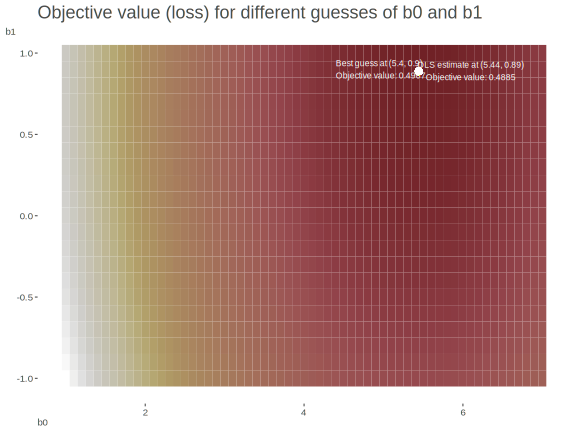
\includegraphics[width=0.5\textwidth,height=\textheight]{index_files/mediabag/img/ols_guesses.pdf}

}

\caption{Results of parameter search}

\end{figure}%

If we inspect our results from the built-in functions, we had estimates
of 5.44 and 0.89 for our coefficients versus the best guess from our
approach of 5.4 and 0.9. These are very similar but not exactly the
same, but this is mostly due to the granularity of our guesses. Even so,
in the end we can see that we get pretty dang close to what our basic
\texttt{lm} or \texttt{statsmodels} functions would get us. Pretty neat!

\begin{tcolorbox}[enhanced jigsaw, opacityback=0, leftrule=.75mm, bottomrule=.15mm, colframe=quarto-callout-color-frame, rightrule=.15mm, breakable, left=2mm, colback=white, arc=.35mm, toprule=.15mm]

\vspace{-3mm}\textbf{Estimation as `Learning'}\vspace{3mm}

Estimation, and/or optimization, can be seen as the process of a model
learning which parameters will best allow the predictions to match the
observed data, and hopefully, predict as-yet-unseen future data. This is
a very common way to think about estimation in machine learning, and it
is a useful way to think about our simple linear model also.

One thing to keep in mind is that it is not a magical process. It takes
good data, a good idea (model), and an appropriate estimation method to
get good results.

\end{tcolorbox}

\section{Optimization}\label{sec-estim-opt}

Before we get into other objective functions, let's think about a better
way to find the best parameters for our model. Rather than just
guessing, we can use a more systematic approach, and thankfully, there
are tools out there to help us. We just use a function like our OLS
function, give it a starting point, and let the algorithms do the rest!
Thanks to some nifty approaches to making better guesses, these tools
eventually arrive at a pretty good set of parameters. Well, they usually
do, but not always- nothing's perfect! But they are pretty good, and
they are a lot better than guessing. Let's see how we can use one of
these tools to find the best parameters for our model.

Previously we created a set of guesses to search over to see which set
of parameters resulted in prediction that matched the data best. What we
did is called a \textbf{grid search}, and it is a bit of a brute force
approach to finding the best fitting model. You can imagine a couple of
unfortunate or problematic scenarios, such as having a very large number
of parameters, or that our specified range doesn't allow us to get to
the right sets of parameters, or we specify a very large range, but the
best fitting model is within a very narrow part of that range. In any of
these cases we waste a lot of time, and may not find an optimal
solution.

In general, we can think of \textbf{optimization} as a way to find the
best parameters for our model. We start with an initial guess, see how
well it does in terms of our objective function, and then try to improve
it with a new guess. We continue to do so until a stopping point is
reached. Here is an example.

\begin{itemize}
\tightlist
\item
  \textbf{Start with an initial guess} for the parameters
\item
  Calculate the objective function given the parameters
\item
  \textbf{Update the parameters} to a new guess (that hopefully improves
  the objective function)
\item
  Calculate the objective function given the new parameters
\item
  \textbf{Repeat} until the improvement is small enough, or we reach the
  desired number of iterations we want to attempt
\end{itemize}

This is what we described before with estimation in general. The key
idea now is how we \emph{update} the old parameters with a new guess at
each iteration. Different \textbf{optimization algorithms} use different
approaches to find the updated parameters. At some point, either the
improvement is no longer practical, often refered to as our
\textbf{tolerance}, or we reach a maximum number of iterations we want
to attempt, and either of these is something we can set ourselves. If we
meet the terms of our objective, we say that our model has
\textbf{converged}. Sometimes, the number of iterations is not enough
for us to reach convergence in terms of tolerance, and we have to try
again with a different set of parameters, a different algorithm, maybe
use some data transformations, or something else.

So let's try it out! Both R and Python offer a function where we can
specify the objective function, and it will try to find the best
parameters for us. It needs several inputs:

\begin{itemize}
\tightlist
\item
  the objective function
\item
  the initial guess for the parameters to get things going
\item
  inputs to the objective function
\item
  options for the optimization process, e.g.~algorithm, maximum number
  of iterations, etc.
\end{itemize}

With these inputs, we'll let the optimization functions do the rest of
the work. We'll also compare our results to the built-in functions to
make sure we're on the right track.

\subsubsection{R}

We'll use the \texttt{optim} function in R.

\begin{verbatim}
our_result = optim(
    par     = c(1, 0),
    fn      = ols,
    X       = df_happiness$life_exp,
    y       = df_happiness$happiness,
    method  = "BFGS", # optimization algorithm
    control = list(   # specify tolerance, max iter, etc. here
        tol   = 1e-6,
        maxit = 500
    )  
)

# our_result
\end{verbatim}

\subsubsection{Python}

We'll use the \texttt{minimize} function in Python.

\begin{verbatim}
from scipy.optimize import minimize

our_result = minimize(
    fun    = ols,
    x0     = np.array([1., 0.]),
    args   = (
        np.array(df_happiness['life_exp']), 
        np.array(df_happiness['happiness'])
    ),
    method = 'BFGS', # optimization algorithm
    tol    = 1e-6,   # tolerance
    options = {
        'maxiter': 500
    }
)

# our_result
\end{verbatim}

\begin{longtable}{lrr}

\caption{\label{tbl-r-optim-ols}Comparison of our results to built-in
function}

\tabularnewline

\toprule
Parameter & Built-in & Our Result \\ 
\midrule\addlinespace[2.5pt]
Intercept & \textcolor[HTML]{404040}{$5.4450$} & \textcolor[HTML]{404040}{$5.4450$} \\ 
Life Exp. Coef. & \textcolor[HTML]{404040}{$0.8880$} & \textcolor[HTML]{404040}{$0.8880$} \\ 
Objective/MSE & \textcolor[HTML]{404040}{$0.4890$} & \textcolor[HTML]{404040}{$0.4890$} \\ 
\bottomrule

\end{longtable}

So our little function and the right tool allows us to come up with the
same thing as base R and \texttt{statsmodels}! I hope you're feeling
pretty good at this point because you should! You just proved you could
do what seemed before to be like magic, but really all it took is just a
little knowledge about some key concepts. Let's try some more!

\begin{tcolorbox}[enhanced jigsaw, opacityback=0, leftrule=.75mm, bottomrule=.15mm, colframe=quarto-callout-color-frame, rightrule=.15mm, breakable, left=2mm, colback=white, arc=.35mm, toprule=.15mm]

\vspace{-3mm}\textbf{A Note on Terminology}\vspace{3mm}

The objective function is often called the \textbf{loss function}, and
sometimes the \textbf{cost function}. However, these both imply that we
are trying to minimize the function, which is not always the
case\footnotemark{}, and it's arbitrary whether you want to minimize or
maximize the function. In fact, some people will minimize the
\emph{negative} likelihood when using \emph{maximum} likelihood! As such
we'll try to stick to the more neutral term `objective function', but
you may see the other terms used interchangeably in this text. In
addition, some packages will use the term \textbf{metric} to refer a
value that you might want to examine as well, or even use to compare
models. For example, the MSE is a metric, but it may also be the
objective function we are trying to minimize. Other metrics we could
calculate without being the objective might be Adjusted R-squared and
mean absolute error. We could also use MSE as the objective, but use
percentage drop in error from baseline when selecting among several
models that minimized MSE. This can be very confusing when starting out!
We'll try to stick to the term \emph{metric} for additional values that
we might want to examine separate from the \emph{objective function
value}.

\end{tcolorbox}

\footnotetext{You may find that some packages will only minimize (or
maximize) a function, possibly one that you come up with yourself. It'd
be nice if they did this internally, or allowed the user to specify the
direction like most packages, but you'll need to take care when
implementing your own metrics.}

\section{Maximum Likelihood}\label{sec-estim-maxlike}

In our example thus far, we have been minimizing the specific objective
(or loss) function, which basically takes our parameter estimates,
produces a prediction, and returns the sum or mean of the squared
errors. But this is just one approach we could take. Now we'd like you
to think about the \textbf{data generating process}. We have a model
that says happiness is a function of life expectancy, but more
specifically, let's think about how the observed value of the happiness
score is generated in a statistical sense. In particular, what kind of
probability distribution might be involved? Ignoring the model, we might
think that each happiness value is generated by some random process, and
that the process is the same for each observation. Let's assume that
random process is a normal distribution. So something like this would
describe it mathematically:

\[
\textrm{happiness} \sim N(\mu, \sigma)
\]

where \(\mu\) is the mean of the happiness and \(\sigma\) is the
standard deviation, or in other words, we can think of happiness as a
random variable that is drawn from a normal distribution with \(\mu\)
and \(\sigma\) as the parameters of that distribution.

Let's apply this idea to our linear model setting. In this case, the
mean is a function of life expectancy, and we're not sure what the
standard deviation is, but we can go ahead and write our model as
follows.

\[
\mu = \beta_0 + \beta_1 * \textrm{life\_exp}
\] \[
\textrm{happiness} \sim N(\mu, \sigma)
\]

Now, we can think of the model as a way to estimate the parameters of
the normal distribution, but we have an additional parameter to
estimate. We still have our previous coefficients, but now we need to
estimate \(\sigma\), which is basically our RMSE, as well. But we still
have to think of things a little differently. When we compare our
prediction to the observed value, we don't look at the simple
difference, but we are still interested in the discrepancy between the
two. So now we think about the \textbf{likelihood} of observing the
happiness score given our prediction, which is based on the estimated
parameters, i.e.~given the \(\mu\) and \(\sigma\), and \(\mu\) is a
function of the coefficients and life expectancy. We can write this as:

\[
\textrm{Pr}(\textrm{happiness} \mid \textrm{life\_exp}, \beta_0, \beta_1, \sigma)
\]

\[
\textrm{Pr}(\textrm{happiness} \mid \mu, \sigma)
\]

Even more generally, the likelihood gives us a sense of the probability
of the observed data given the parameter estimates \(\theta\). \[
\textrm{Pr}(\textrm{Data} \mid \theta)
\]

Here is a simple code demo to get a likelihood in the context of our
model. The values you see are referred to statistically as probability
density values, and they are technically not probabilities, but rather
the probability density, or \textbf{relative likelihood}, at that
observation\footnote{The actual probability of a \emph{specific value}
  is 0, but the probability of a range of values is not 0. You can find
  out more about likelihoods and probabilities at the discussion
  \href{https://stats.stackexchange.com/questions/2641/what-is-the-difference-between-likelihood-and-probability}{here},
  but in general many traditional statistical texts will cover this
  also.}. For your conceptual understanding, if it makes it easier, you
can think of them in the same was as you do probabilities, but just know
that technically they are not.

TODO: UPDATE VALUES WHEN DEMO IS SETTLED

\subsubsection{R}

\begin{verbatim}
# two example life expectancy scores, mean and 1 sd above
life_expectancy = c(0, 1)

# observed happiness scores
happiness = c(4, 5.2)

# predicted happiness with rounded coefs
mu = 5 + 1 * life_expectancy

# just a guess for sigma
sigma = .5

# likelihood for each observation
L = dnorm(happiness, mean = mu, sd = sigma)
L
\end{verbatim}

\begin{verbatim}
[1] 0.1079819 0.2218417
\end{verbatim}

\subsubsection{Python}

\begin{verbatim}
from scipy.stats import norm

# two example life expectancy scores, mean and 1 sd above
life_expectancy = np.array([0, 1])

# observed happiness scores
happiness = np.array([4, 5.2])

# predicted happiness with rounded coefs
mu = 5 + 1 * life_expectancy

# just a guess for sigma
sigma = .5

# likelihood for each observation
L = norm.pdf(happiness, loc = mu, scale = sigma)
L
\end{verbatim}

\begin{verbatim}
array([0.1080, 0.2218])
\end{verbatim}

So, given a guess at the parameters, and an assumption about the
distribution of the data, we can calculate the likelihood of observing
each data point, and sum those up, just like we did with our squared
errors. In theory, we'd deal with the product of each likelihood, but in
practice we sum the log of the likelihood, otherwise values would get
too small for our computers to handle. Here is a corresponding function
we can use to calculate the likelihood of the data given our parameters.
Note that the actual likelihood value returned isn't really
interpretable, just that higher is better from a maximization
standpoint. But we can use it to compare models with different sets of
parameter guesses. Even if our total likelihoods under comparison are
negative, we prefer the model with the relatively higher likelihood. As
we just demonstrated, we'll use \texttt{optim} to help us get good
guesses\footnote{Those who have experience here will notice we aren't
  putting a lower bound on sigma. You typically want to do this
  otherwise you may get nonsensical results. You can do this by using
  the \texttt{lower} parameter in \texttt{optim} with an algorithm that
  uses boundaries, or even more simply by exponentiating the parameter,
  i.e.~\texttt{exp(par{[}1{]})}. Just remember that the returned value
  will be on the log scale, so you'll have to exponentiate it to get to
  the correct scale. We leave this detail out of the code for now to
  keep things simple.}.

\subsubsection{R}

\begin{verbatim}
likelihood = function(par, X, y) {
    X = cbind(1, X)
    # setup
    beta = par[-1] # coefficients
    sigma = exp(par[1]) # error sd, exp keeps positive

    N = nrow(X)

    LP = X %*% beta # linear predictor
    mu = LP # identity link in the glm sense

    # calculate (log) likelihood
    ll = dnorm(y, mean = mu, sd = sigma, log = TRUE)
    -sum(ll) # for minimization
}


our_result = optim(
    par = c(1, 0, 0),
    fn  = likelihood,
    X   = df_happiness$life_exp,
    y   = df_happiness$happiness
)

# our_result
\end{verbatim}

\subsubsection{Python}

\begin{verbatim}
def likelihood(par, X, y):
    # add a column of 1s for the intercept
    X = np.c_[np.ones(X.shape[0]), X]

    # setup
    beta   = par[1:]         # coefficients
    sigma  = np.exp(par[0])  # error sd, exp keeps positive

    N = X.shape[0]

    LP = X @ beta          # linear predictor
    mu = LP                # identity link in the glm sense

    # calculate (log) likelihood
    ll = norm.logpdf(y, loc = mu, scale = sigma) 
    return(-np.sum(ll))

our_result = minimize(
    fun  = likelihood,
    x0   = np.array([1, 0, 0]),
    args = (
        np.array(df_happiness['life_exp']), 
        np.array(df_happiness['happiness'])
    )
)
\end{verbatim}

How would we switch to a maximum likelihood approach using readily
available functions? In both R and Python you can switch to using
\texttt{glm} and \texttt{GLM} respectively as a start. We can use
different likelihoods corresponding to the binomial, poisson and other
distributions. Still other packages would allow even more distributions
for consideration. In general, we choose a distribution that we feel
best reflects the data generating process. For binary targets for
example, we typically would feel a bernoulli or binomial distribution is
appropriate. For count data, we might choose a poisson or negative
binomial distribution. For targets that fall between 0 and 1, we might
go for a beta distribution. There are many distributions, and even when
some might feel more appropriate, we might choose another for
convenience. Some distributions tend toward a normal (a.k.a. gaussian)
distribution depending on various factors, while others are special
cases of more general distributions. For example, the exponential
distribution is a special case of the gamma distribution, and a cauchy
is equivalent to a t distribution with 1 degree of freedom, and the t
tends toward a normal with increasing degrees of freedom. Here is a
visualization of the relationships among some of the more common
distributions Wikipedia (2023).

TODO: fig needs work for pdf

\newpage

\blandscape

\begin{figure}[H]

{\centering \includegraphics{img/distribution_relationships.jpg}

}

\caption{Relationships among some of probability distributions}

\end{figure}%

\elandscape

\newpage

Here are examples of standard GLM functions in R and Python

\subsubsection{R}

\begin{verbatim}
glm(happiness ~ life_exp, data = df_happiness, family = gaussian)
glm(binary_target ~ x1 + x2, data = some_data, family = binomial)
glm(count ~ x1 + x2, data = some_data, family = poisson)
\end{verbatim}

\subsubsection{Python}

\begin{verbatim}
import statsmodels.formula.api as smf

smf.glm(
    'happiness ~ life_exp', 
    data = df_happiness, 
    family = sm.families.Gaussian()
)

smf.glm(
    'binary_target ~ x1 + x2', 
    data = some_data, 
    family = sm.families.Binomial()
)

smf.glm(
    'count ~ x1 + x2', 
    data = some_data, 
    family = sm.families.Poisson()
)
\end{verbatim}

With that in mind, we can compare our result to a built-in function that
has capabilities beyond OLS. As before, we're duplicating the basic glm
result. We show more decimal places on the log likelihood estimate to
prove we aren't getting \emph{exactly} the same result

\setlength{\LTpost}{0mm}

\begin{longtable}{lrr}

\caption{\label{tbl-r-likelihood}Comparison of our results to built-in
function}

\tabularnewline

\toprule
Parameter & Built-in & Our Result \\ 
\midrule\addlinespace[2.5pt]
Intercept & \textcolor[HTML]{404040}{$5.44$} & \textcolor[HTML]{404040}{$5.44$} \\ 
Life Exp. Coef. & \textcolor[HTML]{404040}{$0.89$} & \textcolor[HTML]{404040}{$0.89$} \\ 
Sigma & \textcolor[HTML]{404040}{$0.71$} & \textcolor[HTML]{404040}{$0.70$\textsuperscript{\textit{1}}} \\ 
LogLik (neg) & \textcolor[HTML]{404040}{$118.80$} & \textcolor[HTML]{404040}{$118.80$} \\ 
\bottomrule

\end{longtable}

\begin{minipage}{\linewidth}
\textsuperscript{\textit{1}}Parameter estimate is exponentiated\\
\end{minipage}

Let's think more about what's going on here. It turns out that our
objective function defines a space or surface. We can think of it as a
landscape, and we are trying to find the lowest point on that landscape.
We can then think of our guesses as points on that landscape, and we are
trying to find the lowest point. Let's start get a sense of this with
the following visualization, based on a single parameter. The data is
drawn from Poisson distributed variable with true mean \(\theta=5\). We
note the calculated likelihood increases as we estimate values for
\(\theta\) closer to \(5\), or more precisely, whatever the mean
observed value is for the data. However, with more and more data, the
final ML estimate will converge on the true value. Model estimation
finds that maximum on the curve, and optimization algorithms are the
means to find it.

\begin{figure}[H]

\centering{

\includegraphics{estimation_files/figure-pdf/fig-r-likelihood-plot-1.pdf}

}

\caption{\label{fig-r-likelihood-plot}Likelihood function one parameter}

\end{figure}%

Now let's add a parameter. If we have more than one parameter, we now
have a surfaace to deal with. Given some starting point, an optimization
procedure then travels along the surface looking for a minimum/maximum
point. For simpler settings such as this, we can visualize the
likelihood surface and its minimum point. However, even our simple demo
model has three parameters plus the likelihood, so would be difficult to
visualize without additional complexity. To get around this, we show the
results for an alternate model where happiness is standardized also,
which means the intercept is zero\footnote{Linear regression will settle
  on a line that cuts through the means, and when standardizing the mean
  of the features and target are both zero, so the line goes through the
  origin.}, and we don't have to show that.

TODO: CANT DO INTERACTIVE WITH PDF/LATEX. NEED WORKAROUND.

\begin{figure}[H]

\centering{

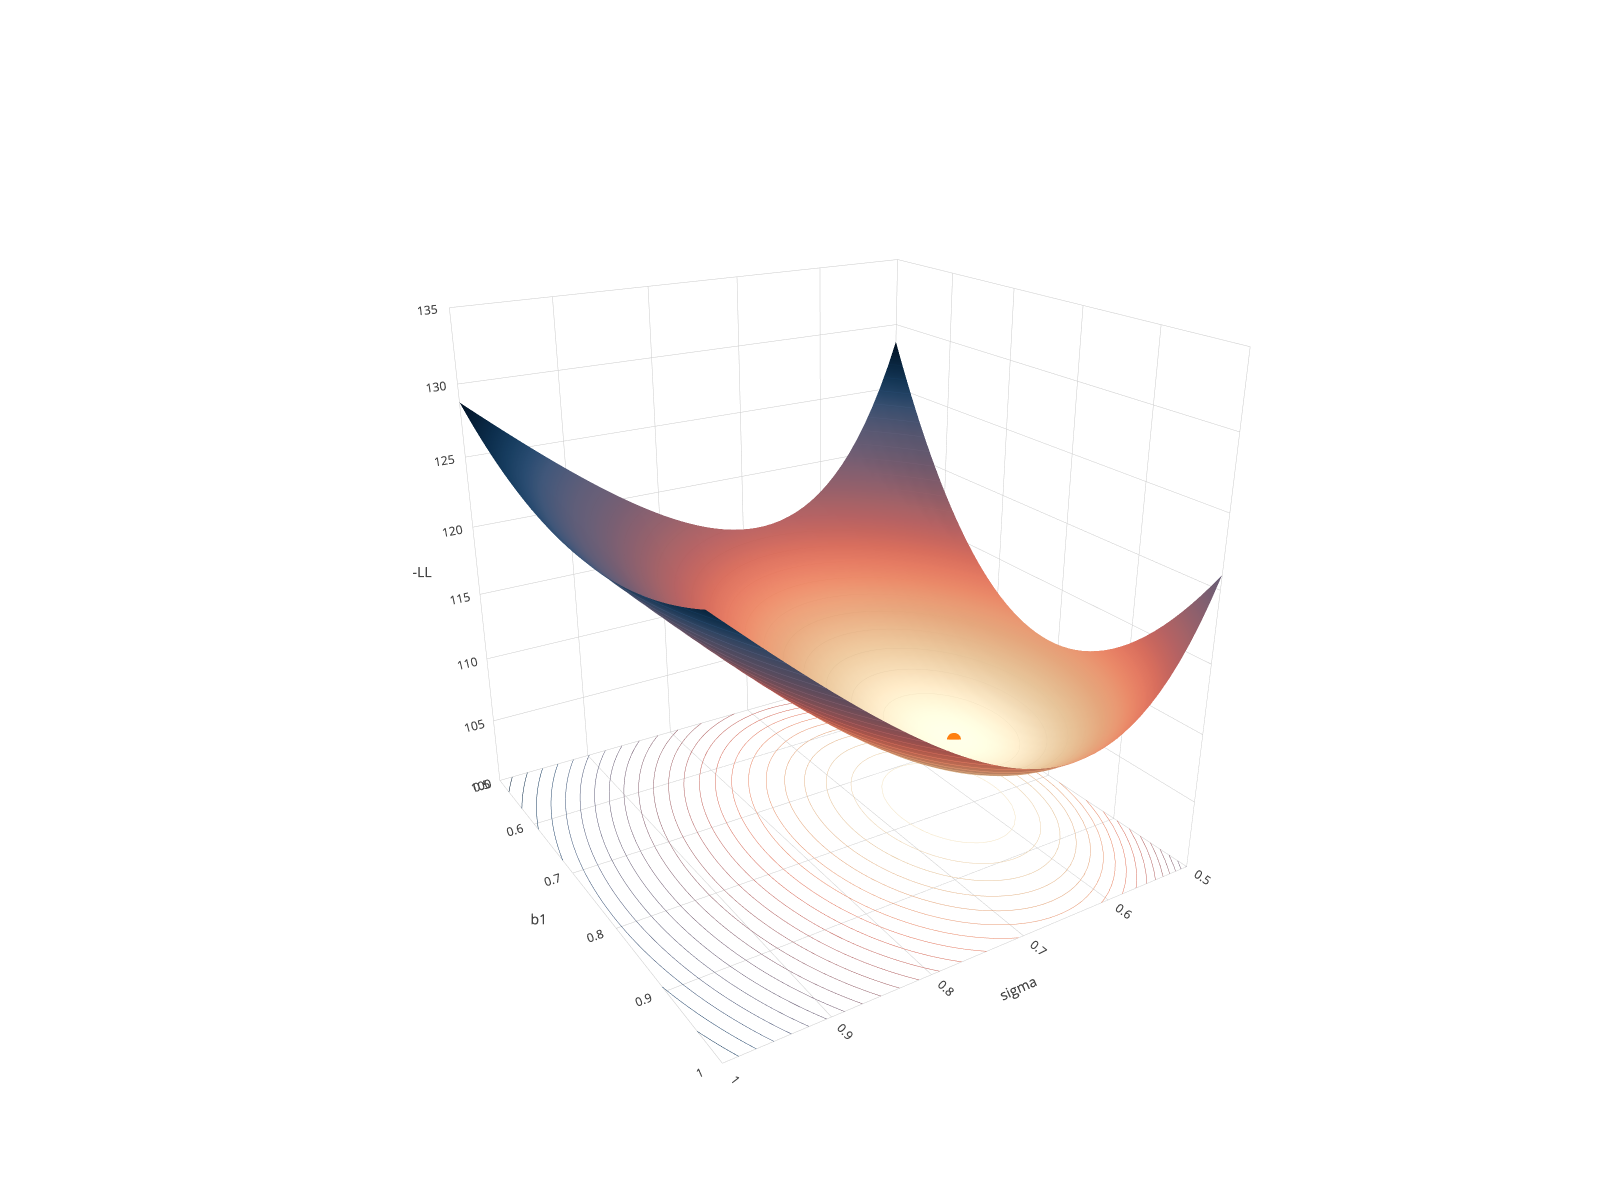
\includegraphics{index_files/mediabag/img/likelihood_surface.pdf}

}

\caption{\label{fig-show-r-likelihood-surface}Likelihood surface for two
parameters}

\end{figure}%

We can also see the path our estimates take, starting at a rather poor
point, but quickly updating to estimates that result in a better
likelihood value. We also see little exploratory jumps creating a star
like pattern, before things ultimately settle to the best values. In
general, these updates and paths are dependent on the optimization
algorithm one uses.

\begin{figure}[H]

\centering{

\includegraphics{estimation_files/figure-pdf/fig-r-likelihood-path-1.pdf}

}

\caption{\label{fig-r-likelihood-path}Optimization path for two
parameters}

\end{figure}%

It turns out that in the case of a normal distribution, the maximum
likelihood estimate of the standard deviation is the estimate as the
standard deviation of the residuals. Furthermore, the maximum likelihood
estimates and OLS estimates converge to the same estimates as the sample
size increases. For any data of significance, these estimates are
indistinguishable, and the OLS estimate is the maximum likelihood
estimate for linear regression.

\subsubsection{Additional Thoughts on Maximum
Likelihood}\label{sec-estim-maxlike-add}

TODO: Remove?

One of the key things to note is that maximum likelihood is an
estimation technique that relies on specifying the probability
distribution that serves as the data generating process. Maximum
likelihood allows us to be explicit about why we think those target
values are the way they are. The likelihood also serves as a fundamental
part of Bayesian analysis, which we'll discuss more later. In general,
maximum likelihood is a powerful technique that can be used in many
contexts, and likelihoods can be used as the objective for many machine
learning algorithms as well.

\section{Estimation: Quick Review}\label{sec-estim-review}

TODO: MOVE WHERE? NEEDED?

At this point we understand a few things:

\begin{itemize}
\tightlist
\item
  Parameters are the values associated with a model
\item
  Objective functions specify a modeling goal with which to estimate the
  parameters.
\item
  Estimation is a way of finding the best model, i.e.~parameters that
  help us achieve a goal.
\item
  Optimization is the process of finding the parameters that maximize or
  minimize some objective function
\item
  The likelihood is an alternate way to assess the match of data and
  model, and allows us to compare the relative fits of models
\end{itemize}

\section{Penalized Objectives}\label{sec-estim-penalty}

TODO: MOVE TO AFTER CLASSIFICATION?

One thing we may want to take into account of with our models is their
complexity, especially in the context of \textbf{overfitting}. We talk
about this with machine learning also, but the basic idea is that we can
get too close to the data we have, such that when we try to predict on
new data, our performance suffers or even gets worse than a simpler
model. In other words, we are not generalizing well. One way to deal
with this is to penalize the objective function value for complexity, or
at least favor simpler models that might do as well. In some contexts
this is called \textbf{regularization}, and in other contexts
\textbf{shrinkage}, since the parameter estimates are typically shrunk
toward some specific value (e.g., zero).

As a starting point, in our basic linear model we can add a penalty that
is applied to the size of coefficients. This is called \textbf{ridge
regression}, or, more mathily, as \textbf{L2 regularization}. The
penalty is just the sum of the squared coefficients multiplied by a some
value, which we call \(\lambda\). We can write this formally as:

\begin{equation}\phantomsection\label{eq-ols-ridge}{
\textrm{Value} = \sum_{i=1}^{n} (y_i - \hat{y_i})^2 + \lambda \sum_{j=1}^{p} \beta_j^2
}\end{equation}

The first part is the same as before (Equation~\ref{eq-ols}), but the
second part is the penalty for \(p\) features. The penalty is the sum of
the squared coefficients multiplied by some value, which we call
\(\lambda\). This is an additional model parameter that we typically
want to estimate in some fashion, e.g.~through cross-validation. This
kind of parameter is often called a hyperparameter, mostly just to
distinguish it from those that may be of actual interest. For example,
we could probably care less what the actual value for \(\lambda\) is,
but we would still be interested in the coefficients.

Interestingly, as you'll notice that this is just OLS+, you might be
wondering how our results or interpretation might change. Well for
starters, L2 regularization is not limited to linear regression, so just
keep that in mind. But also, if we know that OLS produces
\textbf{unbiased} estimates if assumptions of linear regression are met,
that means, if these aren't the same estimates, they must be biased,
right? Your are correct! As we talk about with machine learning
(Section~\ref{sec-ml-generalization}), the bias-variance tradeoff is a
key concept in machine learning, and this is a good example of that. We
are introducing some bias in order to reduce the variance. In other
words, we are willing to accept some bias in order to get a model that
generalizes better.

Another common penalty that is the sum of the absolute value of the
coefficients, which is called \textbf{lasso regression} or \textbf{L1
regularization}. An interersting property of the lasso is that in
typical implementations, it will potentially zero out coefficients,
which is the same as dropping the feature from the model altogether.
This is a form of \textbf{feature selection} or \textbf{variable
selection}. The true values are never zero, but if we want to use a
`best subset' of features, this is one way we could do so. We can write
the lasso objective as:

\begin{equation}\phantomsection\label{eq-estim-lasso}{
\textrm{Value} = \sum_{i=1}^{n} (y_i - \hat{y_i})^2 + \lambda \sum_{j=1}^{p} |\beta_j|
}\end{equation}

But let's get to a code example to make sure we understand this better!
Here is an example of a function that calculates the ridge objective. To
make things interesting, let's add the other features we talked about
regarding GDP per capita and perceptions of corruption.

\subsubsection{R}

\begin{verbatim}
ridge = function(par, X, y, lambda = 0) {
    # add a column of 1s for the intercept
    X = cbind(1, X)

    # Calculate the predicted values
    mu = X %*% par # %*% is matrix multiplication

    # Calculate the value as sum squared error
    error = crossprod(y - mu)

    # Add the penalty
    value = error + lambda * crossprod(par)

    return(value)
}

our_result = optim(
    par = c(0, 0, 0, 0),
    fn = ridge,
    X = df_happiness |> select(-happiness, -country) |> as.matrix(),
    y = df_happiness$happiness,
    lambda = 0.1,
    method = "BFGS"
)
\end{verbatim}

\subsubsection{Python}

\begin{verbatim}
# we use lambda_ because lambda is a reserved word in python
def ridge(par, X, y, lambda_ = 0):
    # add a column of 1s for the intercept
    X = np.c_[np.ones(X.shape[0]), X]

    # Calculate the predicted values
    mu = X @ par
    
    # Calculate the error
    value = np.sum((y - mu)**2)
    
    # Add the penalty
    value = value + lambda_ * np.sum(par**2)
    
    return(value)

our_result = minimize(
    fun  = ridge,
    x0   = np.array([0, 0, 0, 0]),
    args = (
        np.array(df_happiness.drop(columns=['happiness', 'country'])),
        np.array(df_happiness['happiness']), 
        0.1
    )
)
\end{verbatim}

We can compare this to built-in functions as we have before, and can see
that the results are very similar, but not exactly the same. We would
not worry about such differences in practice, but the main point is
again, we can use simple functions that do just about as well as any
what we'd get from package output.

\setlength{\LTpost}{0mm}

\begin{longtable}{lrr}

\caption{\label{tbl-r-ridge}Comparison of ridge regression results}

\tabularnewline

\toprule
Parameter & Built-in\textsuperscript{\textit{1}} & Our Result \\ 
\midrule\addlinespace[2.5pt]
Intercept & \textcolor[HTML]{404040}{$5.44$} & \textcolor[HTML]{404040}{$5.44$} \\ 
Life Exp. Coef. & \textcolor[HTML]{404040}{$0.49$} & \textcolor[HTML]{404040}{$0.52$} \\ 
Corrupt & \textcolor[HTML]{404040}{$-0.12$} & \textcolor[HTML]{404040}{$-0.11$} \\ 
GDP\_PC & \textcolor[HTML]{404040}{$0.42$} & \textcolor[HTML]{404040}{$0.44$} \\ 
\bottomrule

\end{longtable}

\begin{minipage}{\linewidth}
\textsuperscript{\textit{1}}Showing results from R glmnet package with alpha = 0, lambda = .1\\
\end{minipage}

\begin{tcolorbox}[enhanced jigsaw, opacityback=0, leftrule=.75mm, bottomrule=.15mm, colframe=quarto-callout-tip-color-frame, rightrule=.15mm, breakable, left=2mm, colback=white, arc=.35mm, toprule=.15mm]

It turns out that, given a set \(\lambda\) penalty, ridge regression
estimates need not be estimated, as there is an analytical result. See a
\href{https://m-clark.github.io/models-by-example/penalized-maximum-likelihood.htm}{demo}
for more.

\end{tcolorbox}

\section{Classification}\label{sec-estim-classification}

So far we've been assuming a continuous target, but what if we have a
categorical target? Now we have to learn a bunch of new stuff for that
situation, right? Actually, no! \emph{When we want to model categorical
targets, conceptually nothing changes} - we can still have an objective
function that maximizes or minimizes some goal, use the same algorithms
to estimate parameters, etc. However, we need to think about how we can
do this in a way that makes sense for the target.

\subsection{Misclassification}\label{sec-estim-misclass}

A straightforward correspondence to MSE is a function that minimizes
classification error (or maximizes accuracy). In other words, we can
think of the objective function as the proportion of incorrect
classifications. This is called the \textbf{misclassification rate}. We
can write this as:

\[
\textrm{Loss} = \frac{1}{n} \sum_{i=1}^{n} \mathbb{1}(y_i \neq \hat{y_i})
\]

Where \(y_i\) is the actual value of the target for observation \(i\),
arbitrarily coded as 1 or 0, and \(\hat{y_i}\) is the predicted class
from the model. The \(\mathbb{1}\) is an indicator function that returns
1 if the condition is true, and 0 otherwise. In other words, we are
counting the number of times the predicted value is not equal to the
actual value, and dividing by the number of observations. Very
straightforward, so let's do this ourselves!

\subsubsection{R}

\begin{verbatim}
# misclassification rate
misclassification = function(par, X, y, class_threshold = .5) {
    X = cbind(1, X)
    # Calculate the predicted values
    mu = X %*% par # %*% is matrix multiplication

    # Convert to a probability ('sigmoid' function)
    p = 1 / (1 + exp(-mu))

    # Convert to a class
    predicted_class = as.integer(
        ifelse(p > class_threshold, "good", "bad")
    )

    # Calculate the error
    error = y - predicted_class

    return(mean(error))
}
\end{verbatim}

\subsubsection{Python}

\begin{verbatim}
def misclassification_rate(par, X, y, class_threshold = .5):
    # add a column of 1s for the intercept
    X = np.c_[np.ones(X.shape[0]), X]

    # Calculate the predicted values
    mu = X @ par
    
    # Convert to a probability ('sigmoid' function)
    p = 1 / (1 + np.exp(-mu))
    
    # Convert to a class
    predicted_class = np.where(p > class_threshold, 1, 0)
    
    # Calculate the error
    error = y - predicted_class 
    
    return(np.mean(error))
\end{verbatim}

We'll leave it as an exercise to the reader to play around with this, as
the next objective function is more commonly used. But at least you can
see how easy it can be to switch to the classification case.

\subsection{Log loss}\label{sec-estim-logloss}

Another approach is to use the \textbf{log loss}, sometimes called
logistic loss or cross-entropy. If we have just the binary case it is:

\[
\textrm{Loss} = -\sum_{i=1}^{n} y_i \log(\hat{y_i}) + (1 - y_i) \log(1 - \hat{y_i})
\]

Where \(y_i\) is the actual value of the target for observation \(i\),
and \(\hat{y_i}\) is the predicted value from the model (essentially a
probability). It turns out that \emph{this is the same as log-likelihood
used in a maximum likelihood approach for logistic regression}, made
negative for minimization. We typically prefer this objective function
to classification error because it results in a \emph{smooth}
optimization surface, like in the visualization we showed before for
maximum likelihood (Figure~\ref{fig-show-r-likelihood-surface}), which
means it is \emph{differentiable} in mathemetical sense. This is
important because it allows us to use optimization algorithms that rely
on derivatives in updating the parameter estimates. You don't really
need to get into that too much, but just know that it is a good thing.
Here's some code to try out.

\subsubsection{R}

\begin{verbatim}
objective = function(par, X, y) {
    X = cbind(1, X)

    # Calculate the predicted values on the raw scale
    y_hat = X %*% par

    # Convert to a probability ('sigmoid' function)
    y_hat = 1 / (1 + exp(-y_hat))

    # likelihood (or dbinom(y, size = 1, prob = y_hat, log = TRUE))
    ll = y * log(y_hat) + (1 - y) * log(1 - y_hat)

    return(sum(-ll))
}
\end{verbatim}

\subsubsection{Python}

\begin{verbatim}
def objective(par, X, y):
    # add a column of 1s for the intercept
    X = np.c_[np.ones(X.shape[0]), X]

    # Calculate the predicted values
    y_hat = X @ par
    
    # Convert to a probability ('sigmoid' function)
    y_hat = 1 / (1 + np.exp(-y_hat))
    
    # likelihood
    ll = y * np.log(y_hat) + (1 - y) * np.log(1 - y_hat)
    
    return(-np.sum(ll))
\end{verbatim}

Let's go ahead and demonstrate this. Let's go back to our movie review
data, but we'll use a version of our rating where a movie is `good' if
the rating is 3 or greater, and `bad' otherwise, which we have in our
processed version of the data. Our features will be the review year
(starting at zero), reviewer age, and word count. Let's use our previous
optimization functions, and compare our results to the built-in
complements.

\subsubsection{R}

\begin{verbatim}
df_reviews_pr = read_csv("data/movie_reviews_processed.csv")

mod_logloss = optim(
    par = c(0, 0, 0, 0),
    fn = objective,
    X = df_reviews_pr |>
        select(review_year_0, age_sc, word_count_sc) |>
        as.matrix(),
    y = df_reviews_pr$rating_good
)

mod_glm = glm(
    rating_good ~ review_year_0 + age_sc + word_count_sc,
    data   = df_reviews_pr,
    family = binomial
)
\end{verbatim}

\subsubsection{Python}

\begin{verbatim}
from scipy.optimize import minimize

mod_logloss = minimize(
    objective,
    x0 = np.array([0, 0, 0, 0]),
    args = (
        df_reviews_pr[['review_year_0', 'age_sc', 'word_count_sc']], 
        df_reviews_pr['rating_good']
    )
)

mod_glm = smf.glm(
    'rating_good ~ review_year_0 + age_sc + word_count_sc',
    data   = df_reviews_pr,
    family = sm.families.Binomial()
).fit(method = 'lbfgs')
\end{verbatim}

Once again we can see that the results are very similar, but not exactly
the same, though actually have to go out several decimal places before
we start seeing differences between our result and the built-in
function.

\begin{longtable}{lrr}

\caption{\label{tbl-logloss}Comparison of log loss results}

\tabularnewline

\toprule
name & Ours & GLM \\ 
\midrule\addlinespace[2.5pt]
LogLike & \textcolor[HTML]{404040}{$622.5935$} & \textcolor[HTML]{404040}{$622.5935$} \\ 
int & \textcolor[HTML]{404040}{$-0.0819$} & \textcolor[HTML]{404040}{$-0.0818$} \\ 
review\_year\_0 & \textcolor[HTML]{404040}{$0.0213$} & \textcolor[HTML]{404040}{$0.0213$} \\ 
age\_sc & \textcolor[HTML]{404040}{$-0.2213$} & \textcolor[HTML]{404040}{$-0.2213$} \\ 
word\_count\_sc & \textcolor[HTML]{404040}{$-0.7344$} & \textcolor[HTML]{404040}{$-0.7343$} \\ 
\bottomrule

\end{longtable}

So when it comes to classification, you should feel confident in what's
going on under the hood, just like you did with a numeric target.
Conceptually it really is the same approach.

\section{Optimization Algorithms}\label{sec-estim-opt-algos}

When it comes to optimization, there are a number of algorithms that
have been developed over time. We'll demonstate one of the most popular
ones used in machine learning, but there many variants of this one even!
The main thing to keep in mind is that these are all just ways to find
the best fitting parameters for a model. The algorithms differ in how
they do this, and some may be better suited for certain data tasks, or
provide computatational advantages.

\subsection{Gradient Descent}\label{sec-estim-opt-algos-gd}

One of the most common approaches in optimization is called
\textbf{gradient descent}. The idea behind it is that we can use the
gradient of the objective function to guide us to the best fitting
parameters. We still use estimation approaches like maximum likelihood -
gradient descent is just a way to find that path along the objective
surface. More formally, the gradient is the vector of partial
derivatives of the objective function with respect to each parameter.
That may not mean much to you, but the basic idea is that the gradient
is a vector that points in the direction of steepest ascent in terms of
the objective function. So if we want to maximize the objective
function, we can take a step in the direction of the gradient, and if we
want to minimize it, we can take a step in the opposite direction of the
gradient. The size of the step is called the \textbf{learning rate},
and, like our penalty parameter we saw with penalized regression, it is
a hyperparameter that we can tune. If the learning rate is too small, it
will take a longer time to converge. If the learning rate is too large,
we might overshoot the objective and never converge. There are a number
of variations on gradient descent that have been developed over time.
Here is a function to illustrate the process. Let's see this in action
with the happiness data model we used previously.

\subsubsection{R}

\begin{verbatim}
gradient_descent = function(
    par,
    X,
    y,
    tolerance = 1e-3,
    maxit = 1000,
    learning_rate = 1e-3,
    adapt = FALSE,
    verbose = TRUE
) {
    # add a column of 1s for the intercept
    X = cbind(1, X)
    N = nrow(X)

    # initialize
    beta = par
    names(beta) = colnames(X)
    mse = crossprod(X %*% beta - y) / N
    tol = 1
    iter = 1

    while (tol > tolerance && iter < maxit) {
        LP = X %*% beta
        grad = t(X) %*% (LP - y)
        betaCurrent = beta - learning_rate * grad
        tol = max(abs(betaCurrent - beta))
        beta = betaCurrent
        mse = append(mse, crossprod(LP - y) / N)
        iter = iter + 1

        if (adapt) {
            stepsize = ifelse(
                mse[iter] < mse[iter - 1],
                stepsize * 1.2,
                stepsize * .8
            )
        }

        if (verbose && iter %% 10 == 0) {
            message(paste("Iteration:", iter))
        }
    }

    list(
        par    = beta,
        loss   = mse,
        MSE    = crossprod(LP - y) / nrow(X),
        iter   = iter,
        fitted = LP
    )
}

our_result = gradient_descent(
    par = c(0, 0, 0, 0),
    X = df_happiness |> select(life_exp, gdp_pc, corrupt) |> as.matrix(),
    y = df_happiness$happiness,
    learning_rate = 1e-3,
    verbose = FALSE
)
\end{verbatim}

\subsubsection{Python}

\begin{verbatim}
def gradient_descent(
    par, 
    X, 
    y, 
    tolerance = 1e-3, 
    maxit = 1000, 
    learning_rate = 1e-3, 
    adapt = False, 
    verbose = True
):
    # add a column of 1s for the intercept
    X = np.c_[np.ones(X.shape[0]), X]
    
    # initialize
    beta = par
    loss = np.sum((X @ beta - y)**2)
    tol = 1
    iter = 1

    while (tol > tolerance and iter < maxit):
        LP = X @ beta
        grad = X.T @ (LP - y)
        betaCurrent = beta - learning_rate * grad
        tol = np.max(np.abs(betaCurrent - beta))
        beta = betaCurrent
        loss = np.append(loss, np.sum((LP - y)**2))
        iter = iter + 1

        if (adapt):
            stepsize = np.where(
                loss[iter] < loss[iter - 1], 
                stepsize * 1.2, 
                stepsize * .8
            )

        if (verbose and iter % 10 == 0):
            print("Iteration:", iter)

    return({
        "par": beta,
        "loss": loss,
        "RSE": np.sqrt(np.sum((LP - y)**2) / (X.shape[0] - X.shape[1])),
        "iter": iter,
        "fitted": LP
    })

our_result = gradient_descent(
    par = np.array([0, 0, 0, 0]),
    X = df_happiness[['life_exp', 'gdp_pc', 'corrupt']].to_numpy(),
    y = df_happiness['happiness'].to_numpy(),
    learning_rate = 1e-3,
    verbose  = False
)
\end{verbatim}

Comparing our results, we have the following table. In what has become
the norm, we see that the results are very similar.

\begin{longtable}{lrr}

\caption{\label{tbl-gradient-descent}Comparison of gradient descent
results}

\tabularnewline

\toprule
Value & Built-in & Our Result \\ 
\midrule\addlinespace[2.5pt]
Intercept & \textcolor[HTML]{404040}{$5.445$} & \textcolor[HTML]{404040}{$5.437$} \\ 
Life Exp. Coef. & \textcolor[HTML]{404040}{$0.525$} & \textcolor[HTML]{404040}{$0.521$} \\ 
GDP\_PC & \textcolor[HTML]{404040}{$0.438$} & \textcolor[HTML]{404040}{$0.439$} \\ 
Corrupt & \textcolor[HTML]{404040}{$-0.105$} & \textcolor[HTML]{404040}{$-0.107$} \\ 
MSE & \textcolor[HTML]{404040}{$0.367$} & \textcolor[HTML]{404040}{$0.367$} \\ 
\bottomrule

\end{longtable}

In addition, when we visualize the loss function across iterations, we
see smooth decline in the MSE value as we go along each iteration. This
is a good sign that we are converging to a good solution.

\begin{figure}[H]

\centering{

\includegraphics{estimation_files/figure-pdf/fig-r-gradient-descent-1.pdf}

}

\caption{\label{fig-r-gradient-descent}Gradient descent path}

\end{figure}%

\subsection{Stochastic Gradient Descent}\label{sec-estim-opt-algos-sgd}

\textbf{Stochastic gradient descent} (SGD) is a variation on gradient
descent that uses a random sample of the data to estimate the gradient,
while the `true' gradient is the gradient of the objective function with
respect to all of the data. As such, it's less accurate than the `batch'
gradient descent in some sense, but the advantage of SGD is that it is
faster. In practice, SGD is often used in machine learning applications
where the data is large, and the tradeoff between accuracy and speed is
worth it.

Let's see this in action with the happiness data model we used
previously. The following is a conceptual version of the AdaGrad
approach\footnote{MC does not recall exactly where this origin of his
  function came from except that Murphy's PML book was a key reference
  (Murphy (2012)).}, which is a variation of stochastic gradient descent
that adjusts the learning rate for each parameter. We will also add a
variation that averages the parameter estimates across iterations, which
is a common approach to improve the performance of stochastic gradient
descent, but by default it is not used, just something you can play
with. We are going to use a `batch size' of one, which is similar to a
`streaming' or `online' version where we update the model with each
observation. Since our data are alphabetically ordered, we'll shuffle
the data first. We'll also use a stepsize\_tau parameter, which is a way
to adjust the learning rate at early iterations. We'll set it to zero
for now, but you can play with it to see how it affects the results. The
values for the learning rate and stepsize\_tau are arbitrary, selected
after some initial playing around, but you can play with them to see how
they affect the results.

TODO: SHOULD MAYBE CLEAN UP/ALTER TO LESS VERBOSE VERSION

\subsubsection{R}

\begin{verbatim}
stochastic_gradient_descent = function(
    par, # parameter estimates
    X, # model matrix
    y, # target variable
    learning_rate = 1, # the learning rate
    stepsize_tau = 0, # if > 0, a check on the LR at early iterations
    average = FALSE # a variation of the approach
    ) {
    # initialize
    X = cbind(1, X)
    beta = par

    # Collect all estimates
    betamat = matrix(0, nrow(X), ncol = length(beta))

    # Collect fitted values at each point))
    fits = NA

    # Collect loss at each point
    loss = NA

    # adagrad per parameter learning rate adjustment
    s = 0

    # a smoothing term to avoid division by zero
    eps = 1e-8

    for (i in 1:nrow(X)) {
        Xi = X[i, , drop = FALSE]
        yi = y[i]

        # matrix operations not necessary here,
        # but makes consistent with standard gd func
        LP = Xi %*% beta
        grad = t(Xi) %*% (LP - yi)
        s = s + grad^2 # adagrad approach

        # update
        beta = beta - learning_rate / (stepsize_tau + sqrt(s + eps)) * grad

        # a variation
        if (average & i > 1) {
            beta = beta - 1 / i * (betamat[i - 1, ] - beta)
        }

        betamat[i, ] = beta
        fits[i] = LP
        loss[i] = crossprod(LP - yi)
    }

    LP = X %*% beta
    lastloss = crossprod(LP - y)

    list(
        par = beta, # final estimates
        par_chain = betamat, # estimates at each iteration
        MSE = sum(lastloss) / nrow(X),
        fitted = LP
    )
}

# setting a seed ensures replicability
set.seed(123)

# generate random sample indices (could also have done within the function)
idx = sample(1:nrow(df_happiness), nrow(df_happiness))

X_train = df_happiness |>
    select(life_exp, gdp_pc, corrupt) |>
    dplyr::slice(idx) |>
    as.matrix()

y_train = df_happiness$happiness[idx]

our_result = stochastic_gradient_descent(
    par = c(mean(df_happiness$happiness), 0, 0, 0),
    X = X_train,
    y = y_train,
    learning_rate = .15,
    stepsize_tau = .1
)
\end{verbatim}

\subsubsection{Python}

\begin{verbatim}
def stochastic_gradient_descent(
    par, # parameter estimates
    X, # model matrix
    y, # target variable
    learning_rate = 1, # the learning rate
    stepsize_tau = 0, # if > 0, a check on the LR at early iterations
    average = False # a variation of the approach
):
    # initialize
    X = np.c_[np.ones(X.shape[0]), X]
    beta = par

    # Collect all estimates
    betamat = np.zeros((X.shape[0], beta.shape[0]))

    # Collect fitted values at each point))
    fits = np.zeros(X.shape[0])

    # Collect loss at each point
    loss = np.zeros(X.shape[0])

    # adagrad per parameter learning rate adjustment
    s = 0

    # a smoothing term to avoid division by zero
    eps = 1e-8

    for i in range(X.shape[0]):
        Xi = X[None, i, :]
        yi = y[i]

        # matrix operations not necessary here,
        # but makes consistent with standard gd func
        LP = Xi @ beta
        grad = Xi.T @ (LP - yi)
        s = s + grad**2 # adagrad approach

        # update
        beta = beta - learning_rate / \
            (stepsize_tau + np.sqrt(s + eps)) * grad

        # a variation
        if (average & i > 1):
            beta = beta - 1 / i * (betamat[i - 1, :] - beta)

        betamat[i, :] = beta
        fits[i] = LP
        loss[i] = np.sum((LP - yi)**2)

    LP = X @ beta
    lastloss = np.sum((LP - y)**2)

    return({
        "par": beta, # final estimates
        "par_chain": betamat, # estimates at each iteration
        "MSE": lastloss / X.shape[0],
        "fitted": LP
    })

# setting a seed ensures replicability
np.random.seed(1234)

# generate random sample indices (could also have done within the function)
idx = np.random.choice(
    df_happiness.shape[0], 
    df_happiness.shape[0], 
    replace = False
)

X_train = df_happiness[['life_exp', 'gdp_pc', 'corrupt']].to_numpy()[idx, :]
y_train = df_happiness['happiness'].to_numpy()[idx]

our_result = stochastic_gradient_descent(
    par = np.array([np.mean(df_happiness['happiness']), 0, 0, 0]),
    X = X_train,
    y = y_train,
    learning_rate = .15,
    stepsize_tau = .1
)
\end{verbatim}

Next we'll compare it to OLS estimates. Very similar even though SGD
normally would not be used for such a small dataset. We also show our
previous `batch' gradient descent results for comparison.

\begin{longtable}{lrrr}

\caption{\label{tbl-stochastic-gradient-descent}Comparison of stochastic
gradient descent results}

\tabularnewline

\toprule
Value & Built-in & Our Result & Batch SGD \\ 
\midrule\addlinespace[2.5pt]
Intercept & \textcolor[HTML]{404040}{$5.445$} & \textcolor[HTML]{404040}{$5.469$} & \textcolor[HTML]{404040}{$5.437$} \\ 
Life Exp. Coef. & \textcolor[HTML]{404040}{$0.525$} & \textcolor[HTML]{404040}{$0.514$} & \textcolor[HTML]{404040}{$0.521$} \\ 
GDP\_PC & \textcolor[HTML]{404040}{$0.438$} & \textcolor[HTML]{404040}{$0.390$} & \textcolor[HTML]{404040}{$0.439$} \\ 
Corrupt & \textcolor[HTML]{404040}{$-0.105$} & \textcolor[HTML]{404040}{$-0.111$} & \textcolor[HTML]{404040}{$-0.107$} \\ 
MSE & \textcolor[HTML]{404040}{$0.367$} & \textcolor[HTML]{404040}{$0.370$} & \textcolor[HTML]{404040}{$0.367$} \\ 
\bottomrule

\end{longtable}

And here's a plot of the estimates as they moved along the data. For
this plot we don't include the intercept as it's on a notably different
scale. We can see that the estimates are moving around a bit, but they
appear to be converging to a solution.

\begin{figure}[H]

\centering{

\includegraphics{estimation_files/figure-pdf/fig-r-stochastic-gradient-descent-1.pdf}

}

\caption{\label{fig-r-stochastic-gradient-descent}Stochastic gradient
descent path}

\end{figure}%

\subsection{Other Optimization
Algorithms}\label{sec-estim-opt-algos-other}

There are lots of other approaches to optimization. For example, here
are some of the options available in R's \texttt{optim} or scipy's
\texttt{minimize} function:

\begin{itemize}
\tightlist
\item
  Nelder-Mead
\item
  BFGS
\item
  L-BFGS-B (provides constraints)
\item
  Conjugate gradient
\item
  Simulated annealing
\item
  Newton's method
\item
  Genetic algorithms
\end{itemize}

The main reason to choose one method over another usually is some sort
of computational gain, e.g.~memory or speed, or it may just work better
for some types of models in practice. For statistical problems, many
GLM-type functions appear to use Newton's as a default, but more
complicated models may implement a different default for better
convergence. In general, we can always try a few different methods to
see which works best, and often there would be little differences in the
results. For example, here are the results for the happiness model using
different algorithms, with a comparison to the standard linear
regression model function. We can see that the results are very similar,
and for simpler modeling endeavors they should converge on the same
result.

\setlength{\LTpost}{0mm}

\begin{longtable}{lrrrrr}

\caption{\label{tbl-optim-compare}Comparison of optimization results}

\tabularnewline

\toprule
parameter & NM\textsuperscript{\textit{1}} & BFGS\textsuperscript{\textit{2}} & CG\textsuperscript{\textit{3}} & GD\textsuperscript{\textit{4}} & Built-in\textsuperscript{\textit{5}} \\ 
\midrule\addlinespace[2.5pt]
Intercept & \textcolor[HTML]{404040}{$5.445$} & \textcolor[HTML]{404040}{$5.445$} & \textcolor[HTML]{404040}{$5.445$} & \textcolor[HTML]{404040}{$5.437$} & \textcolor[HTML]{404040}{$5.445$} \\ 
Life Exp. Coef. & \textcolor[HTML]{404040}{$0.525$} & \textcolor[HTML]{404040}{$0.525$} & \textcolor[HTML]{404040}{$0.525$} & \textcolor[HTML]{404040}{$0.521$} & \textcolor[HTML]{404040}{$0.525$} \\ 
GDP\_PC & \textcolor[HTML]{404040}{$0.437$} & \textcolor[HTML]{404040}{$0.438$} & \textcolor[HTML]{404040}{$0.438$} & \textcolor[HTML]{404040}{$0.439$} & \textcolor[HTML]{404040}{$0.438$} \\ 
Corrupt & \textcolor[HTML]{404040}{$-0.105$} & \textcolor[HTML]{404040}{$-0.105$} & \textcolor[HTML]{404040}{$-0.105$} & \textcolor[HTML]{404040}{$-0.107$} & \textcolor[HTML]{404040}{$-0.105$} \\ 
MSE & \textcolor[HTML]{404040}{$0.367$} & \textcolor[HTML]{404040}{$0.367$} & \textcolor[HTML]{404040}{$0.367$} & \textcolor[HTML]{404040}{$0.367$} & \textcolor[HTML]{404040}{$0.367$} \\ 
\bottomrule

\end{longtable}

\begin{minipage}{\linewidth}
\textsuperscript{\textit{1}}NM = Nelder-Mead\\
\textsuperscript{\textit{2}}BFGS = Broyden–Fletcher–Goldfarb–Shanno\\
\textsuperscript{\textit{3}}CG = Conjugate gradient\\
\textsuperscript{\textit{4}}GD = Gradient descent\\
\textsuperscript{\textit{5}}Built-In = Standard OLS function\\
\end{minipage}

\section{Other Estimation Approaches}\label{sec-estim-other}

Before leaving our estimation discussion, we should mention that there
are other approaches to estimation that are out there, some quite
common. These include variaions on least squares, \textbf{method of
moments}, \textbf{generalized estimating equations}, \textbf{robust}
estimation, and more. The above that we've focused on will generally be
sufficient for most applications, but it's good to be aware of others.
But there are two we want to discuss in a little bit detail before we
leave model estimation formally given their widespread usage, and that
is the \textbf{bootstrap} and \textbf{Bayesian estimation}.

\subsection{Bootstrap}\label{sec-estim-bootstrap}

The \textbf{bootstrap} is a resampling approach to estimation. We
\textbf{sample with replacement} from the data observations, generating
an entirely new data set of the same size, and then estimate the model.
We repeat this process many times, collecting parameter estimates,
predictions, or any thing we want to calculate along the way. Ultimately
we end up with a distribution of possible parameter estimates, metrics,
and whatever else we calculated.

This distribution is useful for \textbf{inference}\footnote{We're using
  inference here in the statistical/philosophical sense, not as a
  synonym for prediction or generalization, which is how it is often
  used in machine learning. We're not exactly sure how that
  terminological muddling arose in ML, but be on the lookout for it.},
as we can use the distribution to calculate confidence intervals,
prediction intervals or intervals for anything we happen to calculate.
The average estimate will typically be the same as whatever the
underlying model used would produced, but the bootstrap provides a way
to get at a measure of \textbf{uncertainty} with fewer assumptions about
how that distribution should take shape. The bootstrap is very flexible,
and it can be used with any estimation approach, let's see this in
action with the happiness data model we used previously.

\subsubsection{R}

\begin{verbatim}
bootstrap = function(X, y, nboot = 100, seed = 123) {
    # add a column of 1s for the intercept
    N = nrow(X)

    # initialize
    beta = matrix(NA, (1+ncol(X))*nboot, nrow = nboot, ncol = 1+ncol(X))
    colnames(beta) = c('Intercept', colnames(X))
    mse = rep(NA, nboot)

    # set seed
    set.seed(seed)

    for (i in 1:nboot) {
        # sample with replacement
        idx = sample(1:N, N, replace = TRUE)
        Xi = X |> slice(idx)
        yi = y[idx]

        # estimate model
        mod = lm(yi ~., data = Xi)

        # save results
        beta[i, ] = coef(mod)
        mse[i] = sum((mod$fitted - yi)^2) / N
    }

    # given mean estimates, calculate MSE
    y_hat = cbind(1, as.matrix(X)) %*% colMeans(beta)
    final_mse = sum((y - y_hat)^2) / N

    list(
        beta = as_tibble(beta),
        MSE = mse,
        final_mse = final_mse
    )
}

our_result = bootstrap(
    X = df_happiness |> select(life_exp, gdp_pc, corrupt),
    y = df_happiness$happiness,
    nboot = 250
)
\end{verbatim}

\subsubsection{Python}

\begin{verbatim}
def bootstrap(X, y, nboot=100, seed=123):
    cn = X.columns
    # add a column of 1s for the intercept
    X = np.c_[np.ones(X.shape[0]), X]
    N = X.shape[0]

    # initialize
    beta = np.empty((nboot, X.shape[1]))
    
    # beta = pd.DataFrame(beta, columns=['Intercept'] + list(cn))
    mse = np.empty(nboot)    

    # set seed
    np.random.seed(seed)

    for i in range(nboot):
        # sample with replacement
        idx = np.random.randint(0, N, N)
        Xi = X[idx, :]
        yi = y[idx]

        # estimate model
        model = LinearRegression(fit_intercept=False)
        mod = model.fit(Xi, yi)

        # save results
        beta[i, :] = mod.coef_
        mse[i] = np.sum((mod.predict(Xi) - yi)**2) / N

    # given mean estimates, calculate MSE
    y_hat = X @ beta.mean(axis=0)
    final_mse = np.sum((y - y_hat)**2) / N

    return dict(beta = beta, mse = mse, final_mse = final_mse)

our_result = bootstrap(
    X = df_happiness[['life_exp', 'gdp_pc', 'corrupt']],
    y = df_happiness['happiness'],
    nboot = 250
)
\end{verbatim}

Here are the results of the interval estimates for the coefficients. For
each parameter, we have the mean estimate, the lower and upper bounds of
the 95\% confidence interval, and the width of the interval. We can see
that the bootstrap intervals are wider than the OLS intervals, possibly
better capturing the uncertainty in this model based on not too many
observations.

\setlength{\LTpost}{0mm}

\begin{longtable}{lrrrrrr}

\caption{\label{tbl-bootstrap}Bootstrap parameter estimates}

\tabularnewline

\toprule
Parameter & mean & Lower BS & Upper BS & Lower OLS & Upper OLS & Diff Width\textsuperscript{\textit{1}} \\ 
\midrule\addlinespace[2.5pt]
Intercept & \textcolor[HTML]{404040}{$5.44$} & \textcolor[HTML]{404040}{$5.33$} & \textcolor[HTML]{404040}{$5.55$} & \textcolor[HTML]{404040}{$5.33$} & \textcolor[HTML]{404040}{$5.56$} & \textcolor[HTML]{404040}{$-0.02$} \\ 
life\_exp & \textcolor[HTML]{404040}{$0.51$} & \textcolor[HTML]{404040}{$0.30$} & \textcolor[HTML]{404040}{$0.70$} & \textcolor[HTML]{404040}{$0.35$} & \textcolor[HTML]{404040}{$0.70$} & \textcolor[HTML]{404040}{$0.04$} \\ 
gdp\_pc & \textcolor[HTML]{404040}{$0.46$} & \textcolor[HTML]{404040}{$0.18$} & \textcolor[HTML]{404040}{$0.76$} & \textcolor[HTML]{404040}{$0.24$} & \textcolor[HTML]{404040}{$0.64$} & \textcolor[HTML]{404040}{$0.18$} \\ 
corrupt & \textcolor[HTML]{404040}{$-0.10$} & \textcolor[HTML]{404040}{$-0.29$} & \textcolor[HTML]{404040}{$0.09$} & \textcolor[HTML]{404040}{$-0.25$} & \textcolor[HTML]{404040}{$0.04$} & \textcolor[HTML]{404040}{$0.09$} \\ 
\bottomrule

\end{longtable}

\begin{minipage}{\linewidth}
\textsuperscript{\textit{1}}Width of bootstrap estimate minus width of OLS estimate\\
\end{minipage}

Let's look more closely at the bootstrap distributions for each
coefficient. With standard statistical estimates, we are assuming a
distribution like the normal, which is a very specific shape. With the
bootstrap, we can be more flexible, though often it may tend toward the
distribution that would otherwise be assumed anyway. These aren't
perfectly symmetrical, but they suit our needs in that we can extract
the lower and upper quantiles to create an interval estimate.

\begin{figure}[H]

\centering{

\includegraphics{estimation_files/figure-pdf/fig-r-bootstrap-1.pdf}

}

\caption{\label{fig-r-bootstrap}Bootstrap distributions of parameter
estimates}

\end{figure}%

The bootstrap is a commonly used for predictions and other metrics, but
it is computationally inefficient, and can become prohibitive with large
data sizes. Also, the simple bootstrap will likely not estimate the
appropriate uncertainty for some types of statistics (e.g.~extreme
values) or
\href{https://stats.stackexchange.com/questions/9664/what-are-examples-where-a-naive-bootstrap-fails}{in
some data contexts} (e.g.~correlated observations). Overcoming the
limitations may typically require an even more computationally intensive
approach, further limiting its utility. But it is a useful tool to have
in your toolbox, and it can be used in conjunction with other approaches
to get at uncertainty in a model.

\subsection{Bayesian Estimation}\label{sec-estim-bayes}

The \textbf{Bayesian} approach to modeling is a philosophical viewpoint,
an entirely different way to think about probability, a different way to
measure uncertainty, and on a practical level, just another way to get
model parameter estimates. It can be as frustrating as it is fun to use,
and one of the really nice things about using Bayesian estimation is
that it can handle model complexities that other approaches don't do
well.

The basis of Bayesian estimation is the \textbf{likelihood}, the same as
used with maximum likelihood, and everything we did there follows to
here. However, here we can incorporate domain knowledge about the
parameters, in the form of \textbf{prior distributions}, which we
specify in addition to the likelihood. For example, we may say that the
coefficients for a linear model come from a normal distribution centered
on zero with some variance. The combination prior distributions with the
likelihood ultimately results in the \textbf{posterior distribution}.
And this is the key difference when comparing Bayesian estimation to the
others we've talked about, and something it shares in common with the
bootstrap- the end result is not a point estimate of the parameters, but
rather a \emph{distribution} of possible parameter values.

\includegraphics{img/prior2post_clean.png}

Dealing with distributions instead of single estimates is a different
way to think about modeling, but it can be very useful. For example, as
we did with the bootstrap, the Bayesian posterior distribution is useful
for inference. With these distributions, we can look at any range in
between for our \textbf{credible interval}, which is the Bayesian
equivalent of a confidence interval\footnote{Your default interpretation
  of a standard confidence interval is almost certaintly, and
  incorrectly, the actual interpretation of a Bayesian confidence
  interval, because the Bayesian interpretation of confidence intervals
  and p-values is how we tend to naturally think about them. But that's
  okay, everyone else is in the same boat. We also don't care if you
  want to call the Bayesian version a credible interval or a confidence
  interval.}. Here is an example of the posterior distribution for the
parameters of our happiness model, along with 95\% intervals.

\begin{figure}[H]

\centering{

\includegraphics{estimation_files/figure-pdf/fig-r-bayesian-posterior-1.pdf}

}

\caption{\label{fig-r-bayesian-posterior}Posterior distribution of
parameters}

\end{figure}%

With Bayesian modeling, we use the algorithm of our choosing, give it
starting values and proceed much in the same way as other optimization
procedures. However, in this approach, we always specify a number of
iterations as the \textbf{stopping rule}, i.e.~when the model should
terminate. These iterations are single draws from the posterior
distribution for each parameter. So if we specified 1000 iterations, we
would have 1000 draws from the posterior distribution for each
parameter. Typically we don't use the first few hundred draws, as these
are considered \textbf{burn-in} or \textbf{warmup} draws, and we use the
remaining draws for inference. The number of burn-in draws is a bit of
an art, but it's not too important as long as it's not too small. The
more iterations we set, the longer it will take to run. We also specify
multiple \textbf{chains}, which are each doing the exact same thing, but
do to the random nature of the Bayesian approach, would take different
estimation paths. We can then compare the chains to see if they are
converging to the same result, which is a check on the model. If they
are not converging, we may need to run the model longer, or we may need
to change something else. Here is an example of the chains for our
happiness model for the life expectancy coefficient. We can see that
they are converging to the same result, so we are good to go. Nowadays
we have simple metrics that allow us to check whether the chains are
converging, making it easier to assess many parameters quickly.

\begin{figure}[H]

\centering{

\includegraphics{estimation_files/figure-pdf/fig-r-bayesian-chains-1.pdf}

}

\caption{\label{fig-r-bayesian-chains}Bayesian chains for life
expectancy coefficient}

\end{figure}%

When we are interested in making predictions, we can use the results to
generate a distribution of possible predictions \emph{for each
observation}, which can be very useful when we want to quantify
uncertainty in for complex models. This is referred to as
\textbf{posterior predictive distribution}. Here is a plot of several
draws of predicted values against the true happiness scores.

\begin{figure}[H]

\centering{

\includegraphics{estimation_files/figure-pdf/fig-r-bayesian-posterior-predictive-1.pdf}

}

\caption{\label{fig-r-bayesian-posterior-predictive}Posterior predictive
distribution of happiness values}

\end{figure}%

Note that \emph{any} metric we can calculate from a model will also have
a distribution. For example, you have a classification model and you
want to know the accuracy or true positive rate of the model. Instead of
a single number, you now have access to a whole distribution of values
for that metric. Why? For every sample of the distribution of
parameters, you generate a prediction, convert it a class and compare it
to the true class. So now you have a posterior predictive distribution
for the predicted probabilities and class, and you can then calculate
the accuracy, area under a receiver operating curve, true positive rate,
etc., for each sample, and you have a distribution of possible values.
As an example, we did this for our happiness model and show the interval
estimate for R-squared. Pretty neat!

\setlength{\LTpost}{0mm}

\begin{longtable}{rrr}

\caption{\label{tbl-r-bayesian-metrics}Bayesian R\textsuperscript{2}}

\tabularnewline

\toprule
Bayes R2 & Lower & Upper \\ 
\midrule\addlinespace[2.5pt]
\textcolor[HTML]{404040}{$0.71$} & \textcolor[HTML]{404040}{$0.65$} & \textcolor[HTML]{404040}{$0.75$} \\ 
\bottomrule

\end{longtable}

\begin{minipage}{\linewidth}
95\% Credible interval for R-squared\\
\end{minipage}

\begin{tcolorbox}[enhanced jigsaw, opacityback=0, leftrule=.75mm, bottomrule=.15mm, colframe=quarto-callout-tip-color-frame, rightrule=.15mm, breakable, left=2mm, colback=white, arc=.35mm, toprule=.15mm]

There is nothing keeping you from doing posterior predictive checks with
other estimation approaches, and it's a good idea to do so. For example,
in a GLM you have the beta estimates and the covariance matrix for them,
and can simulate from a normal distribution with those estimates. But
it's a bit more straightforward with the Bayesian approach, and some
packages will allow you to do this automatically even.

\end{tcolorbox}

\subsubsection{Additional Thoughts}\label{additional-thoughts}

It turns out that any standard (frequentist) statistical model can be
seen as a Bayesian one from a particular point of view. Here are a
couple:

\begin{itemize}
\tightlist
\item
  GLM and related estimated via maximum likelihood: Bayesian estimation
  with a flat/uniform prior on the parameters.
\item
  Ridge Regression: Bayesian estimation with a normal prior on the
  coefficients, penalty parameter is related to the variance of the
  prior
\item
  Lasso Regression: Bayesian estimation with a Laplace prior on the
  coefficients, penalty parameter is related to the variance of the
  prior
\end{itemize}

So in many modeling contexts, you're actually doing a restrictive form
of Bayesian estimation already. Hopefully this helps to demystify the
Bayesian approach a bit, and you feel more comfortable switching to it.
R has excellent tools here for modeling and post-processing, like brms
and tidybayes, and Python has pymc3, numpyro, and arviz, which are also
useful\footnote{Honestly R has way more going on here, with many
  packages devoted to Bayesian estimation of specific models even, but
  if you want to stick with Python for it you at least have some
  options. Stan, a probabilistic language underlying many of the
  packages in R, has tools there as well, but they are not nearly as
  well developed or test in Python.}.

We can see that the Bayesian approach is very flexible, and can be used
for many different types of models, and can be used to get at
uncertainty in a model in ways that other approaches can't. It's not a
panacea, and it's not always the best approach, but it's a good one to
have in your toolbox.

TODO: WHERE TO PUT THIS PRIOR STUFF? DELETE!?

The tough part about the Bayesian approach is specifying priors, but
even when you don't have a great idea, many have offered solutions, and
there are ways to check whether what you've chosen makes sense for your
data before trying the model itself.

\begin{tcolorbox}[enhanced jigsaw, opacityback=0, leftrule=.75mm, bottomrule=.15mm, colframe=quarto-callout-tip-color-frame, rightrule=.15mm, breakable, left=2mm, colback=white, arc=.35mm, toprule=.15mm]

Specification of priors can be done in different ways, and nowadays,
there is a lot of information on how to do so, and with some tools, it's
also pretty straightforward to check whether the priors are sensible
without even running a model. When you do have actual prior knowledge,
either domain knowledge (e.g.~a prior study found the beta values to be
positive), statistical knowledge, (e.g.~only the largest standard
coefficients go near or beyond 1), data from time periods, there's
typically at least something to help you specify your priors with
sensible values. This takes away most of the luster of the primary
argument against the Bayesian approach, which is the subjective nature
of priors. But there is likewise so much subjective decision making in
other approaches, that it's not really a useful argument to begin with.
The Bayesian approach just makes it more explicit. And if you don't have
any prior knowledge, you can use non- or weakly- informative priors,
which will likely have little influence and let the data do the talking,
producing a result that is not that different from maximum likelihood
estimation.

\end{tcolorbox}

\section{Wrapping Up}\label{sec-estim-wrap}

Wow, we covered a lot here! But this is the sort of stuff that can take
you from just having some fun with data, to doing that and also
understanding how things are actually happening. Just having the gist of
how modeling actually is done `under the hood' makes so many other
things make sense, and can give you a lot of confidence, even in less
familiar modeling domains.

\section{Where to Go From Here}\label{sec-estim-where-to-go}

Really, after this chapter, you should feel fine with any of the others,
so dive in! Here are some additional resources to consider.

\section{Exercise}\label{exercise-1}

Try creating an objective function for a continuous target that uses the
mean absolute error, and compare your estimated parameters to the
previous results.

TODO: refs need work!

\textbf{OLS and Maximum Likelihood Estimation}:

For OLS and maximum likelihood estimation, there are so many resources
out there, we recommend just taking a look and seeing which one suits
you best. Practically any more technical statistical book will cover
these topics in detail.

\begin{itemize}
\tightlist
\item
  \href{https://stats.stackexchange.com/questions/33197/advanced-statistics-books-recommendation}{A
  list of classical references}
\item
  TODO: recent?
\end{itemize}

\textbf{Gradient Descent}:

\begin{itemize}
\tightlist
\item
  \href{https://www.youtube.com/watch?v=sDv4f4s2SB8}{Gradient Descent,
  Step-by-Step} StatQuest with Josh Starmer (2019a)
\item
  \href{https://www.youtube.com/watch?v=vMh0zPT0tLI}{Stochastic Gradient
  Descent, Clearly Explained} StatQuest with Josh Starmer (2019b)
\end{itemize}

The simple AdaGrad algorithm used above:

\begin{itemize}
\tightlist
\item
  Brownlee (2021)
\item
  DataBricks (2019)
\end{itemize}

\textbf{Bootstrap}: ?

\textbf{Bayesian}:

\begin{itemize}
\tightlist
\item
  BDA Gelman et al. (2013)
\item
  Statistical Rethinking McElreath (2020)
\item
  \href{https://github.com/stan-dev/stan/wiki/Prior-Choice-Recommendations}{Choosing
  priors}
\end{itemize}

\chapter{Generalized Linear Models}\label{sec-glm}

What happens when your target variable isn't really a continuous
variable, but is instead some other type of response. Maybe you've got a
binary condition, like good or bad, or maybe you've got a count of
something, like the number of times a person has been arrested. In these
cases, you can use a linear regression, but it often won't do exactly
what you want. But you can use a \textbf{generalized linear model} to
help yourself in these situations.

Generalized linear models exist to map different distributions into
linear space. This allows us to use the same linear model framework that
we've been using, but with different types of data.

These models work by \textbf{generalizing} the linear model to different
distributions of the target variable. Our coefficients will certainly
take on a new meaning; so while we cannot interpret them as we would
coefficients from a linear regression, we can still use the general
framework.

\section{Key Ideas}\label{sec-glm-key}

\begin{itemize}
\tightlist
\item
  A simple tweak to our previous approach allows us to generalize are
  linear model to account for other settings.
\item
  Common distributions such as binomial, poisson, and others can often
  do better for us both in terms of model fit and interpretability.
\item
  Getting familiar with just a couple distributions will allow you to
  really expand your modeling repertoire.
\end{itemize}

\subsection{Why this matters}\label{sec-glm-why}

The linear model is powerful on its own, but even more so when you
realize you can extend many other data settings, some of which are
implicitly nonlinear! When we want to classify observations, count them,
or deal with proportions and other things, simple tweaks of our standard
linear model allow us to handle such situations.

\subsection{Good to know}\label{sec-glm-good2know}

Generalized linear models are a broad class of models that extend the
linear model to different distributions of the target variable. In
general, you'd need to have a pretty good grasp of linear regression
before getting too carried away here.

\section{Distributions \& Link Functions}\label{sec-glm-distributions}

Remember how linear models really enjoy the whole Gaussian distribution
scene? The essential form of the linear model can be expressed as
follows:

\[
\mu = \alpha + X\beta
\] \[
y \sim \textrm{Normal}(\mu,\sigma)
\]

Not all data follows a Gaussian distribution. Instead, we often find
some other form of an exponential distribution. So, we need a way to
incorporate different distributions of the target into our model.
Distributions cannot do it alone! We also need a \textbf{link function}
to connect the linear model to the distribution.

From a theoretical perspective, link functions are tricky to get your
head around.

\begin{itemize}
\tightlist
\item
  \emph{Find the exponential of the response's density function and
  derive the canonical link function}\ldots{}
\end{itemize}

From a conceptual perspective, all they are doing is allowing the linear
feature to ``link'' to a distribution function's mean. If you know a
distribution's canonical link function, that is all the deeper you will
probably every need.

At the end of the day, these link functions will convert the target to
an unbounded continuous variable. The take-away here is that the link
function describes how the mean is generated from the predictors.

\section{Logistic Regression}\label{sec-glm-logistic}

\subsection{Why Should You Care}\label{sec-glm-logistic-why}

You will often have a binary variable that you might want to use as a
target -- it could be dead/alive, lose/win, quit/retain, etc. You might
be tempted to use a linear regression, but you will quickly find that it
is not the best option. You are going to be figuring out the probability
of moving from ``failure'' to ``success'', given the features in your
model.

TODO: can probably move distribution part of this section to appendix as
part of general discussion of some distributions worth knowing, esp.~as
this is focused on binomial as a count, and the model focus is on the
binary/bernoulli special case.

\subsection{The Binomial Distribution}\label{sec-glm-binomial}

Logistic regression is substantially different than linear regression.
It is also a bit confusing, because it is named after its link function
(\textbf{logit}) instead of its distribution (\textbf{binomial}).
Instead of that nice continuous target, we are dealing with a
binomially-distributed target and the target takes the form of a binary
variable.

We don't have a \(\mu\) or \(\sigma^2\) to identify the shape of the
binomial distribution; instead we have \emph{p} and \emph{n}, where
\emph{p} is a probability and \emph{n} is the number of trials. We tend
to talk about \emph{p} with regard to the probability of a specific
event happening (heads, wins, defaulting, etc.).

Let's see how the binomial distribution looks with 100 trials and
probabilities of ``success'' at \emph{p = } .25, .5, and .75:

\begin{figure}[H]

\centering{

\includegraphics{generalized_linear_models_files/figure-pdf/fig-binomial-1.pdf}

}

\caption{\label{fig-binomial}Binomial distributions for different
probabilities}

\end{figure}%

If we examine the distribution for a probability of .5 in
Figure~\ref{fig-binomial}, we will see that it is centered over 50 --
this would suggest that we have the highest probability of encountering
50 successes if we ran 100 trials. If we run 100 trials 100 times and
the outcome is 50/50, the most common outcome from those 100 trials
would be 50 successes. with a decreasing probability of observing more
or less successes as we move away from 50. Shifting our attention to a
.75 probability of success, we see that our density is sitting over 75.
Again running 100 trials, would give us the highest probability of
observing 75 successes. Some of those 100 trials produce more or less
than 75 successes, but with lower probabilities as you get further away
from 75.

Since we are dealing with a number of trials, it is worth noting that
the binomial distribution is a discrete distribution. If you have any
interest in knowing the probability for a number of success under the
binomial distribution, we can use the following formula:

\[P(x) = \frac{n!}{(n-x)!x!}p^xq^{n-x}\]

While we don't need to dive into finding those specific values for the
binomial distribution, we can spend our time exploring how it looks in
linear model space:

\[
\textrm{logit}(p) = \alpha + X\beta
\]

\[y \sim \textrm{Binomial}(n, p) \\ \]

The \emph{logit} function is defined as:

\[\textrm{log}\frac{p}{1-p}\]

We are literally just taking the log of the odds (the log odds becomes
important later).

Now we can map this back to our model:

\[\textrm{log}\frac{p}{1-p} = \alpha + X\beta\]

And finally we can take that logistic function and invert it (the
\textbf{inverse-logit}) to produce the probabilities.

\[p = \frac{\textrm{exp}(\alpha + X\beta)}{1 + \textrm{exp}(\alpha + X\beta)}\]

Whenever we get coefficients for the logistic regression model, we are
always going to get them as log odds. We can exponentiate them to get
the odds ratio, but we can also exponentiate them and divide by 1 + that
value to get the probability.

\subsection{Probability, Odds, and Log
Odds}\label{sec-glm-binomial-prob}

Probability lies at the heart of all of this. We can look at the
relationship between the probability, odds, and log odds. We can start
with a set of probability values where \(0 < p > 1\)

With that list of probability values, we can convert them to odds with
\(\\p\, / 1 - p\).

\begin{figure}[H]

\centering{

\includegraphics{generalized_linear_models_files/figure-pdf/fig-odds-log-odds-1.pdf}

}

\caption{\label{fig-odds-log-odds}Log odds and odds values for a range
of probabilities}

\end{figure}%

We can see how those probability values map to odds in
Figure~\ref{fig-odds-log-odds}.

Now, we can take those odds values and convert them to log odds.

\begin{figure}[H]

\centering{

\includegraphics{generalized_linear_models_files/figure-pdf/fig-prob-log-odds-1.pdf}

}

\caption{\label{fig-prob-log-odds}Log odds and probability values}

\end{figure}%

If you've ever seen the sigmoid featured in
Figure~\ref{fig-prob-log-odds} before, it is the classic logistic
function!

We can clearly go back and forth between the 3, but the main message
here is that we took a bounded variable in probability and transformed
it to continuous space.

We will see more about how this happens after playing with the model.

\subsection{Data Import and
Preparation}\label{data-import-and-preparation}

We are going to return to our movie reviews data and we are going to use
\texttt{rating\_good} as our target. Before we get to modeling, see if
you can find out the frequency of ``good'' and ``bad'' reviews. We will
use \texttt{word\_count} and \texttt{gender} as our predictors. Before
we move on, though, find the probability of getting a ``good'' review.

TODO: change import to \texttt{df\_reviews} and proceed accordingly.
Leave model fitting via optim to estimation chapter

\subsubsection{R}

\begin{verbatim}
reviews = read.csv("data/movie_reviews_processed.csv")
\end{verbatim}

\begin{verbatim}
X = reviews[, c("word_count", "gender")]

X = cbind(1, X)

X$gender = ifelse(X$gender == "male", 1, 0)

X = as.matrix(X)

y = reviews$rating_good
\end{verbatim}

\subsubsection{Python}

\begin{verbatim}
import pandas as pd


reviews = pd.read_csv("data/movie_reviews_processed.csv")
\end{verbatim}

\begin{verbatim}
X = reviews[['word_count', 'gender']]

y = reviews["rating_good"]
\end{verbatim}

\subsection{Standard Functions}\label{sec-glm-binomial-standard}

To get started with our first logistic regression model, let's use the
\texttt{glm} function from R and Python's \texttt{statsmodels} function.

\subsubsection{R}

\begin{verbatim}
model_logistic = glm(
    rating_good ~ word_count + gender, 
    data = reviews,
    family = binomial
)

summary(model_logistic)
\end{verbatim}

\begin{verbatim}

Call:
glm(formula = rating_good ~ word_count + gender, family = binomial, 
    data = reviews)

Coefficients:
            Estimate Std. Error z value Pr(>|z|)    
(Intercept)  1.71240    0.18136   9.442   <2e-16 ***
word_count  -0.14639    0.01551  -9.436   <2e-16 ***
gendermale   0.11891    0.13751   0.865    0.387    
---
Signif. codes:  0 '***' 0.001 '**' 0.01 '*' 0.05 '.' 0.1 ' ' 1

(Dispersion parameter for binomial family taken to be 1)

    Null deviance: 1370.4  on 999  degrees of freedom
Residual deviance: 1257.4  on 997  degrees of freedom
AIC: 1263.4

Number of Fisher Scoring iterations: 4
\end{verbatim}

\subsubsection{Python}

\begin{verbatim}
import statsmodels.api as sm

X = sm.add_constant(X)

X = pd.get_dummies(X, drop_first = True)

model_logistic = sm.Logit(y, X.astype(float)).fit()
\end{verbatim}

\begin{verbatim}
Optimization terminated successfully.
         Current function value: 0.628697
         Iterations 5
\end{verbatim}

\begin{verbatim}
model_logistic.summary()
\end{verbatim}

\begin{verbatim}
<class 'statsmodels.iolib.summary.Summary'>
"""
                           Logit Regression Results                           
==============================================================================
Dep. Variable:            rating_good   No. Observations:                 1000
Model:                          Logit   Df Residuals:                      997
Method:                           MLE   Df Model:                            2
Date:                Wed, 28 Feb 2024   Pseudo R-squ.:                 0.08245
Time:                        18:31:54   Log-Likelihood:                -628.70
converged:                       True   LL-Null:                       -685.19
Covariance Type:            nonrobust   LLR p-value:                 2.925e-25
===============================================================================
                  coef    std err          z      P>|z|      [0.025      0.975]
-------------------------------------------------------------------------------
const           1.7124      0.181      9.442      0.000       1.357       2.068
word_count     -0.1464      0.016     -9.436      0.000      -0.177      -0.116
gender_male     0.1189      0.138      0.865      0.387      -0.151       0.388
===============================================================================
"""
\end{verbatim}

\subsection{Interpretation and
Visualization}\label{sec-glm-binomial-interpret}

We need to know what those results mean. The coefficients that we get
from our model are in log odds. We can exponentiate them to get the odds
ratio, but we can also exponentiate them and divide by 1 + that value to
get the probability. Interpretting log odds is a fool's errand, but we
can at least get a feeling for them directionally. A log odds of 0 would
indicate no relationship between the feature and target. A positive log
odds would indicate that an increase in the feature will increase the
log odds of moving from ``bad'' to ``good'', whereas a negative log odds
would indicate that a decrease in the feature will decrease the log odds
of moving from ``bad'' to ``good''. We can convert those log odds to
help make some more sense from them.

When we exponentiate the log odds coefficients, we are given the odds
ratio. This is the ratio of the odds of the outcome (i.e., success from
our binomial distribution) occurring for a one unit increase in the
predictor.

\begin{verbatim}
(Intercept)  word_count  gendermale 
  5.5422663   0.8638229   1.1262687 
\end{verbatim}

Fortunately, the intercept is easy -- it is the odds of a ``good''
review when word count is 0 and gender is ``female''. We see that we've
got an odds ratio of .86 for the word\_count variable and 1.12 for the
male variable. An odds ratio of 1 means that there is no change in the
odds of the outcome occurring -- essentially that the predictor does not
influence the target. An odds ratio of less than 1 means that the odds
of the outcome occurring decrease as the predictor increases (while a
bit more complicated to wrap your head around, it captures the idea of
the odds of moving from a ``bad'' review to a ``good'' review
decreasing). An odds ratio of greater than 1 means that the odds of the
outcome occurring increase as the predictor increases (again, the odds
of moving from a ``bad'' review to a ``good'' review increasing).

It is far more intuitive to interpret the probability. We can do this by
exponentiating the coefficients and dividing by 1 + that value. This
will give us the probability of the outcome occurring for a one unit
increase in the predictor.

\begin{verbatim}
(Intercept)  word_count  gendermale 
  0.8471478   0.4634683   0.5296925 
\end{verbatim}

We would say that our probability of moving from a ``bad'' review to a
``good'' review is .84 when there are 0 words in the review and the
gender is female. Since word\_count is below .5, we know that it will
have a negative relationship with the probability of moving from ``bad''
to ``good''; being a male reviewer will have a positive relationship
with the probability of moving from ``bad'' to ``good''.

And visualizing those probabilities is absolutely the best way to see
how the features influence the target:

TODO: Use output to make a better visual, also use \texttt{see} over
\texttt{sjPlot}

\begin{figure}[H]

\centering{

\includegraphics{generalized_linear_models_files/figure-pdf/fig-logistic-regression-count-1.pdf}

}

\caption{\label{fig-logistic-regression-count}Logistic regression
predictions for word count feature}

\end{figure}%

In Figure~\ref{fig-logistic-regression-count}, we can see a clear
negative relationship between the number of words in a review and the
probability of being considered a ``good'' movie. As we get over 20
words, the predicted probability of being a ``good'' movie is less than
.2.

TODO: Use output to make a better visual

\begin{figure}[H]

\centering{

\includegraphics{generalized_linear_models_files/figure-pdf/fig-logistic-regression-gender-1.pdf}

}

\caption{\label{fig-logistic-regression-gender}Logistic regression
predictions for gender feature}

\end{figure}%

In Figure~\ref{fig-logistic-regression-count}, we can see a clear
negative relationship between the number of words in a review and the
probability of being considered a ``good'' movie. As we get over 20
words, the predicted probability of being a ``good'' movie is less than
.2. It does not appear that \texttt{gender} has much of an effect on the
probability of being a ``good'' movie, since the curves are very similar
to each other.

There are interesting issues at play here with regard to our predictor
coefficients (what can be considered a \emph{relative effect}) and the
model's effect as a whole on the probability (the \emph{absolute
effect}). In circumstances where the intercept is very large
(essentially promising a success), the relative effect of a coefficient
is practically meaningless. Similarly, very negative coefficients render
the relative effects useless.

\subsection{Objective Function}\label{sec-glm-binomial-objective}

Let's see how we can pick that work apart to create our own functions.
We can use maximum likelihood estimation to estimate the parameters of
our model.

\subsubsection{R}

\begin{verbatim}
logreg_ml = function(par, X, y) {
  beta = par
  N = nrow(X)
  LP = X %*% beta                           
  mu = plogis(LP)                           
  L = dbinom(y, size = 1, prob = mu, log = TRUE)   
  -sum(L)                                   
}
\end{verbatim}

\subsubsection{Python}

\begin{verbatim}
def logreg_ml(par, X, y):
    beta = par
    N = X.shape[0]
    LP = X.dot(beta).to_numpy()  
    mu = [1 / (1 + np.exp(-x)) for x in LP]
    mu_minus_1 = [1 - x for x in mu]
    L = y*np.log(mu) + (1 - y)*np.log(mu_minus_1)   
    return -np.sum(L)   
  
\end{verbatim}

\subsection{Model Fitting}\label{sec-glm-binomial-fitting}

Now that we have our objective function, we can fit our model. We will
use the \texttt{optim} function in R and the \texttt{minimize} function
in Python.

\subsubsection{R}

\begin{verbatim}
init = rep(0, ncol(X))

names(init) = c('intercept', 'b1', 'b2')

fit_ml = optim(
  par = init,
  fn  = logreg_ml,
  X   = X,
  y   = y,
  control = list(reltol = 1e-8)
)

pars_ml = fit_ml$par

pars_ml
\end{verbatim}

\begin{verbatim}
 intercept         b1         b2 
 1.7121816 -0.1463750  0.1189308 
\end{verbatim}

\subsubsection{Python}

\begin{verbatim}
import numpy as np
from scipy.optimize import minimize

init = np.zeros(X.shape[1])

fit_ml = minimize(
    fun = logreg_ml,
    x0 = init,
    args = (X, y),
    method = 'BFGS',
    options = {'disp': True}
)
\end{verbatim}

\begin{verbatim}
Optimization terminated successfully.
         Current function value: 628.696593
         Iterations: 11
         Function evaluations: 68
         Gradient evaluations: 17
\end{verbatim}

\begin{verbatim}
fit_ml.x
\end{verbatim}

\begin{verbatim}
array([ 1.71240414, -0.14638763,  0.11891015])
\end{verbatim}

TODO: move one of these so we don't have back-to-back

\begin{tcolorbox}[enhanced jigsaw, opacityback=0, leftrule=.75mm, bottomrule=.15mm, colframe=quarto-callout-important-color-frame, rightrule=.15mm, breakable, left=2mm, colback=white, arc=.35mm, toprule=.15mm]

In theory, there is no such thing as 0 or 1 probability. When your model
encounters such a value, you may receive a warning, but not an error.
The most likely cause of this warning is \textbf{separation}: a variable
is perfectly separating the target. In other words, once a feature gets
below/above a certain value, the target is always 0/1. This can often be
caused by very extreme feature values, interaction groups with very
small sample sizes, or even accidentally including a function of your
target as a feature. More evidence of separation comes when you see your
log odds coefficients return something comically large.

\end{tcolorbox}

\begin{tcolorbox}[enhanced jigsaw, opacityback=0, leftrule=.75mm, bottomrule=.15mm, colframe=quarto-callout-warning-color-frame, rightrule=.15mm, breakable, left=2mm, colback=white, arc=.35mm, toprule=.15mm]

Logistic regression does not have an \(R^2\) value in the way that a
linear regression model does. Instead, there are pseudo-\(R^2\) values,
but they are not the same as the \(R^2\) value that you are used to
seeing. Here is a great breakdown of different pseudo methods.

\end{tcolorbox}

\section{Poisson Regression}\label{sec-glm-poisson}

\subsection{Why Should You Care}\label{sec-glm-poisson-why}

Like logistic regression, poisson regression belongs to a broad class of
generalized linear models. Poisson regression is used when you have a
count variable as your target. The nature of a count variable is very
different, since it starts at 0 and can only be a whole number. We need
a model that will not produce negative predictions and poisson
regression will do that for us.

\subsection{The Poisson
Distribution}\label{sec-glm-poisson-distribution}

The Poisson distribution is very similar to the binomial distribution,
but has some key differences. The biggest difference is in its
parameter: Poisson has a single parameter noted as \(\lambda\). This
rate parameter is going to estimate the expected number of events during
a time interval. This can be accidents in a year, pieces produced in a
day, or hits during the course of a baseball season. We can find the
rate by determining the number of events per interval, multiplied by the
interval length.

\[\frac{\text{event}}{\text{interval}}*\text{interval length} \]

To put some numbers to that, if we have 1 accident per week in a factory
and we are observing a whole year, we would have a rate of
\((1 / 7) * 28 = 4\) accidents per month.

Let's see what that particular distribution might look like in
Figure~\ref{fig-poisson-distribution}:

\begin{figure}[H]

\centering{

\includegraphics{generalized_linear_models_files/figure-pdf/fig-poisson-distribution-1.pdf}

}

\caption{\label{fig-poisson-distribution}Poisson distribution for a rate
of 4}

\end{figure}%

We can also see what it looks like for different rates (some places
might be safer than others) in
Figure~\ref{fig-poisson-distribution-rates}:

\begin{figure}[H]

\centering{

\includegraphics{generalized_linear_models_files/figure-pdf/fig-poisson-distribution-rates-1.pdf}

}

\caption{\label{fig-poisson-distribution-rates}Poisson distributions for
different rates}

\end{figure}%

\begin{tcolorbox}[enhanced jigsaw, opacityback=0, leftrule=.75mm, bottomrule=.15mm, colframe=quarto-callout-note-color-frame, rightrule=.15mm, breakable, left=2mm, colback=white, arc=.35mm, toprule=.15mm]

A cool thing about these distributions is that they can deal with
different \emph{exposure} rates. You don't need observations recorded
over the same interval length, because you can adjust for them
appropriately. They can also be used to model inter-arrival times and
time-until events.

\end{tcolorbox}

Let's make a new variable that will count the number of times a person
uses a personal pronoun word.

\subsubsection{R}

\begin{verbatim}
reviews$poss_pronoun = stringr::str_count(
  reviews$review_text, 
  "\\bI\\b|\\bme\\b|\\b[Mm]y\\b|\\bmine\\b|\\bmyself\\b"
)
\end{verbatim}

\subsubsection{Python}

\begin{verbatim}
reviews['poss_pronoun'] = reviews['review_text'].str.count(
  "\\bI\\b|\\bme\\b|\\b[Mm]y\\b|\\bmine\\b|\\bmyself\\b"
  )
\end{verbatim}

\subsection{The (Sometimes) Thin Line}\label{sec-glm-thinline}

Let's think long and hard about our target variable and what it actually
might be. Since Poisson regression gets its name from the Poisson
distribution, we should probably see if it follows the Poisson
distribution.

\begin{verbatim}

     Goodness-of-fit test for poisson distribution

                      X^2 df  P(> X^2)
Likelihood Ratio 2.283728  3 0.5156453
\end{verbatim}

This is a \(\chi^2\) to test if the distribution deviates from a
Poisson. If we see a statistically significant value, we would say that
it deviates from the tested distribution. In this case, it is pretty
clear that \texttt{poss\_pronoun} could come from a Poisson
distribution.

We can also plot that test using a hanging rootogram:

TODO: convert to ggplot

\begin{figure}[H]

\centering{

\includegraphics{generalized_linear_models_files/figure-pdf/fig-poisson-test-1.pdf}

}

\caption{\label{fig-poisson-test}Hanging rootogram for Poisson
distribution}

\end{figure}%

In Figure~\ref{fig-poisson-test}, the bars are the observed counts and
the red line/points are the fitted counts (i.e., how many would be
expected). If a bar does not reach the 0 line, then the model would
over-predict for that particular count; if the bar dips below the 0
line, the model under-predicts that count. It looks like we are pretty
close for our counts.

\subsection{Standard Functions}\label{sec-glm-poisson-standard}

Recall that every distribution has a link function (or several) that
tend to work well for it. The poisson distribution uses a log link
function:

\[\text{log}(\lambda) = \alpha + X\beta\]
\[y = \textrm{Poisson}(\lambda)\]

Using the log link keeps the outcome positive (we cannot deal with
negative counts). Logs, as they are prone to do, are going to tend
towards an exponential relationship; just be sure that it makes sense
over the entire range of your data.

\subsubsection{R}

\begin{verbatim}
model_poisson = glm(
  poss_pronoun ~ word_count,
  data = reviews,
  family = poisson
)

summary(model_poisson)
\end{verbatim}

\begin{verbatim}

Call:
glm(formula = poss_pronoun ~ word_count, family = poisson, data = reviews)

Coefficients:
             Estimate Std. Error z value Pr(>|z|)    
(Intercept) -1.848982   0.099409  -18.60   <2e-16 ***
word_count   0.103126   0.006433   16.03   <2e-16 ***
---
Signif. codes:  0 '***' 0.001 '**' 0.01 '*' 0.05 '.' 0.1 ' ' 1

(Dispersion parameter for poisson family taken to be 1)

    Null deviance: 996.21  on 999  degrees of freedom
Residual deviance: 776.19  on 998  degrees of freedom
AIC: 1699.7

Number of Fisher Scoring iterations: 5
\end{verbatim}

\begin{verbatim}
exp(model_poisson$coefficients)
\end{verbatim}

\begin{verbatim}
(Intercept)  word_count 
  0.1573974   1.1086314 
\end{verbatim}

\subsubsection{Python}

\begin{verbatim}
import statsmodels.api as sm
import statsmodels.formula.api as smf

model_poisson = smf.glm(
  formula = "poss_pronoun ~ word_count",
  data = reviews,
  family = sm.families.Poisson()
).fit()

model_poisson.summary()        
\end{verbatim}

\begin{verbatim}
<class 'statsmodels.iolib.summary.Summary'>
"""
                 Generalized Linear Model Regression Results                  
==============================================================================
Dep. Variable:           poss_pronoun   No. Observations:                 1000
Model:                            GLM   Df Residuals:                      998
Model Family:                 Poisson   Df Model:                            1
Link Function:                    Log   Scale:                          1.0000
Method:                          IRLS   Log-Likelihood:                -847.83
Date:                Wed, 28 Feb 2024   Deviance:                       776.19
Time:                        18:31:56   Pearson chi2:                     717.
No. Iterations:                     5   Pseudo R-squ. (CS):             0.1975
Covariance Type:            nonrobust                                         
==============================================================================
                 coef    std err          z      P>|z|      [0.025      0.975]
------------------------------------------------------------------------------
Intercept     -1.8490      0.099    -18.599      0.000      -2.044      -1.654
word_count     0.1031      0.006     16.030      0.000       0.091       0.116
==============================================================================
"""
\end{verbatim}

\begin{verbatim}
np.exp(model_poisson.params)
\end{verbatim}

\begin{verbatim}
Intercept     0.157397
word_count    1.108631
dtype: float64
\end{verbatim}

We are going to interpret this almost the same as a linear regression.
The slight wrinkle here, though, is that we are looking at the log
counts (remember that we specified the log link function). In other
words, an increase in one one review word leads to an expected log count
increase of \textasciitilde.01. Just like our logisitc regression, we
could exponentiate this to get 1.108 -- every added word in a review
gets us a \textasciitilde1\% increase in the number of possessive
pronouns. Let's see what this looks like in action in
Figure~\ref{fig-poisson-regression}:

\begin{figure}[H]

\centering{

\includegraphics{generalized_linear_models_files/figure-pdf/fig-poisson-regression-1.pdf}

}

\caption{\label{fig-poisson-regression}Poisson regression predictions
for word count feature}

\end{figure}%

With everything coupled together, we have a meaningful coefficient for
\texttt{word\_count}, a clear plot, and adequate model fit. Therefore,
we might conclude that there is a positive relationship between number
of words in a review on the number of times a person uses a personal
possessive.

\begin{verbatim}

    Overdispersion test

data:  model_poisson
z = -8.0493, p-value = 1
alternative hypothesis: true dispersion is greater than 1
sample estimates:
dispersion 
 0.7606014 
\end{verbatim}

The dispersion value that we see returned (0.7606014 in our case) should
be under 1. A dispersion value over 1 means that we have overdispersion.
Our dispersion value, coupled with our high \emph{p}-value, indicates
that we would fail to reject the null hypothesis of equidispersion.

We can also look back to our model results to compare our residual
deviance to our residual deviance degrees of freedom; if our deviance is
greater than our degrees of freedom, we might have an issue with
overdispersion. Since we are just a bit over and our overdispersion
tests do not indicate any huge issue, we can be relatively okay with our
model. If we had some more extreme overdispersion, we would want to flip
to a quasi-poisson distribution -- our coefficients would not change,
but we would have improved standard errors.

\subsection{Model Specification}\label{sec-glm-poisson-spec}

TODO: Need some text here

\subsubsection{R}

\begin{verbatim}
pois_ll = function(y, X, par) {
  beta = par
  lambda = exp(beta%*%t(X))
  loglik = -sum(dpois(y, lambda, log = TRUE))
  return(loglik)
}
\end{verbatim}

\subsubsection{Python}

\begin{verbatim}
from scipy.stats import poisson

def pois_ll(par, X, y):
    beta = par
    lambda_ = np.exp(X.dot(beta))
    loglik = -np.sum(poisson.logpmf(y, lambda_))
    return loglik
\end{verbatim}

\subsection{Model Fitting}\label{sec-glm-poisson-fitting}

\subsubsection{R}

\begin{verbatim}
form = as.formula("poss_pronoun ~ word_count")
model = model.frame(form, data = reviews)
X = model.matrix(form, data = reviews)
y = model.response(model)

starts = c(0, 0)

fit = optim(
  par = starts ,
  fn  = pois_ll,
  X   = X,
  y   = y,
  method  = "BFGS",
  hessian = TRUE
)

fit$par
\end{verbatim}

\begin{verbatim}
[1] -1.8487431  0.1031103
\end{verbatim}

\subsubsection{Python}

\begin{verbatim}
X = np.column_stack((np.ones(reviews.shape[0]), reviews[['word_count']]))

y = reviews["poss_pronoun"]

init = np.zeros(X.shape[1])

fit = minimize(
  fun = pois_ll,
  x0 = init,
  args = (X, y),
  method = 'BFGS'
)


fit.x
\end{verbatim}

\begin{verbatim}
array([-1.84898106,  0.10312625])
\end{verbatim}

\section{Wrapping Up}\label{sec-glm-wrap}

These are just two of the many models that fall under the broad umbrella
of generalized linear models. Depending on your data situation, you
might want to keep Table~\ref{tbl-glm-models} in mind:

\begin{longtable}{ll}

\caption{\label{tbl-glm-models}Targets and distributions for generalized
linear models}

\tabularnewline

\toprule
Target & Distribution \\ 
\midrule\addlinespace[2.5pt]
Proportions & binomial/beta \\ 
Exponential response & gamma \\ 
3+ categories & multinomial \\ 
Count & poisson/negative binomial \\ 
\bottomrule

\end{longtable}

That is, however, just a tiny slice of the potential distributions that
you might find yourself needing to use in a similar way. While not all
are considered official `generalized linear models', the approach is the
same. While you could always use the general linear model, the key is to
understand the distribution of your target and then find the appropriate
link function to connect it to the linear model. Using the proper
distribution will yield better results and get your model a little
closer to the answer you seek.

\section{Additional Resources}\label{sec-glm-resources}

In any given graduate coursework, you might find a whole semester
dedicated to GLMs. We've only scratched the surface here, but there are
some great resources out there to help you dig deeper. If you are
itching for a text book, there isn't any shortage of them out there and
you can essentially take your pick. If you are looking for something a
bit more applied to get you going, you might want to check out Roback
and Legler's \emph{Beyond Multiple Linear Regression}, available for
free at \url{https://bookdown.org/roback/bookdown-BeyondMLR/}.

\chapter{Extending the Linear Model}\label{sec-lm-extend}

With just linear model and generalized linear models, we have a solid
foundation for modeling, and we've seen how there is a notable amount we
can do with a conceptually simple approach. We've also seen how we can
extend the linear model to handle different types of target
distributions to help us understand and make some inferences about the
relationships between our features and target.

In this chapter, we want to show you how to extend the linear model even
further with still common tools. These particular methods are also good
examples of how we can think about our data and approach in different
ways, and can serve as a good starting point for even more techiques you
may want to explore in the future. A thread that binds these techniques
together is the ability to use a linear model to explore nonlinear
relationships!

\section{Key Ideas}\label{sec-lm-extend-key-ideas}

\begin{itemize}
\tightlist
\item
  The linear and generalized linear models are great and powerful
  starting points for modeling, but there's even more we can do!
\item
  \textbf{Linear models can be used to model nonlinear feature-target
  relationships}
\item
  Various technqiues are availabel allow us to model relationships that
  are not linear or monotonic, and can help us to better understand our
  data, even while still being linear models.
\item
  While these seem like very different approaches, we can still use our
  linear model concepts and approach at the core, take similar
  estimation steps, and even have similar, albeit more, interpretation.
\end{itemize}

\subsection{Why this matters?}\label{sec-lm-extend-why}

The linear model is a great starting point for modeling. It is a simple
approach that can be used to model a wide variety of relationships
between features and targets, and it's also a great way to get a feel
for how to think about modeling. But linear and generalized models are
just the starting point, and the models depicted here are very common
extensions used in a variety of disciplines and industries. More
generally, the following techniques allow for nonlinear realationships
will still employing a linear model approach. This is a very powerful
combination, and it's good to be aware of these tools.

\subsection{Good to know}\label{sec-lm-extend-good}

While these models are extensions of the linear model, they are not
necessarily more complex, but it can take a bit more effort to
interpret. You likely want to be fairly comfortable with standard linear
models at least before you start to explore these extensions.

TODO: This can be a chapter with a general focus on nonlinearities:
intearctions in general and mixed model, gam (effects vary with self or
other), quantile (effects vary with target). Also remind GLM as
introducing nonlinearity.

\section{Interactions}\label{sec-lm-interactions}

Things can be quite complex in a typical model with multiple features,
but just adding features may not be enough to capture the complexity of
the relationships between features and target. Sometimes, we need to
consider how features interact with each other to better understand the
relationships between features and target. A common way to add
complexity in linear models is through \textbf{interactions}. This is
where we allow the effect of a feature to vary depending on the values
of another feature, or even itself!

As a conceptual example, we might expect that the effect of the number
of children in the home on a movie's rating is different for movies from
different genres (much higher for kids movies, maybe lower for horror
movies), or that genre and season work together in some way to affect
rating (e.g.~action movies get higher ratings in summer). We might also
consider that the length of a movie might plateau or even have a
negative effect on rating after a certain point, i.e., it would have a
\textbf{curvilinear} effect. All of these are types of interactions we
can explore. Interactions allow us to incorporate nonlinear
relationships into the model, and so greatly extend the linear model's
capabilities - we basically get to use a linear model in a nonlinear
way!

With that in mind, let's explore how we can add interactions to our
models. Going with our first example, let's see how having kids impacts
the relationship between genre and rating. We'll start with a standard
linear model, and then add an interaction term. Using a formula approach
makes it very straightforward to add an interaction term. We just need
to add a \texttt{:} between the two features we want to interact.

\subsubsection{R}

\begin{verbatim}
df_reviews = read_csv("data/movie_reviews_processed.csv")

model_base = lm(rating ~ children_in_home + genre, data = df_reviews)
model_interaction = lm(rating ~ children_in_home * genre, data = df_reviews)

# summary(model_interaction)
\end{verbatim}

\subsubsection{Python}

\begin{verbatim}
import pandas as pd
import statsmodels.formula.api as smf

df_reviews = pd.read_csv("data/movie_reviews_processed.csv")

model_base = smf.ols(
  formula = 'rating ~ children_in_home + genre', 
  data = df_reviews
).fit()

model_interaction = smf.ols(
  formula = 'rating ~ children_in_home * genre', 
  data = df_reviews
).fit()

model_interaction.summary()
\end{verbatim}

Here is a quick look at the model output for the interaction vs.~no
interaction interaction model. Starting with the base model, the
coefficients look like what we've seen before, but we have several
coefficients for genre. The reason is that genre is composed of several
categories, and converted to a set of dummy variables (refer to
Section~\ref{sec-lm-categorical-features} and
Section~\ref{sec-data-cat}). In the base model, the intercept tells us
what the mean is for the reference group, in this case Action/Adventure,
and the genre coefficients tell us the difference between the mean for
that genre and the reference. For example, the mean rating for
Action/Adventure is 2.76, and the difference between that genre rating
for the drama genre is 0.55. Adding the two gives us the mean for drama
movies 2.76 + 0.55 = 3.32. We also have the coefficient for the numbre
of children in the home, and this does not vary by genre.

\begin{longtable}{lrr}

\caption{\label{tbl-model-interaction-output}Model coefficients with
interaction}

\tabularnewline

\toprule
feature & coef\_base & coef\_inter \\ 
\midrule\addlinespace[2.5pt]
(Intercept) & \textcolor[HTML]{404040}{$2.7640$} & \textcolor[HTML]{404040}{$2.7641$} \\ 
children\_in\_home & \textcolor[HTML]{404040}{$0.1422$} & \textcolor[HTML]{404040}{$0.1419$} \\ 
genreComedy & \textcolor[HTML]{404040}{$0.6350$} & \textcolor[HTML]{404040}{$0.6371$} \\ 
genreDrama & \textcolor[HTML]{404040}{$0.5539$} & \textcolor[HTML]{404040}{$0.5352$} \\ 
genreHorror & \textcolor[HTML]{404040}{$0.1288$} & \textcolor[HTML]{404040}{$0.1938$} \\ 
genreKids & \textcolor[HTML]{404040}{$-0.1990$} & \textcolor[HTML]{404040}{$-0.2759$} \\ 
genreOther & \textcolor[HTML]{404040}{$0.0288$} & \textcolor[HTML]{404040}{$0.0836$} \\ 
genreRomance & \textcolor[HTML]{404040}{$0.2275$} & \textcolor[HTML]{404040}{$0.2981$} \\ 
genreSci-Fi & \textcolor[HTML]{404040}{$-0.1227$} & \textcolor[HTML]{404040}{$-0.1090$} \\ 
children\_in\_home:genreComedy & \textcolor[HTML]{404040}{} & \textcolor[HTML]{404040}{$-0.0060$} \\ 
children\_in\_home:genreDrama & \textcolor[HTML]{404040}{} & \textcolor[HTML]{404040}{$0.0534$} \\ 
children\_in\_home:genreHorror & \textcolor[HTML]{404040}{} & \textcolor[HTML]{404040}{$-0.1274$} \\ 
children\_in\_home:genreKids & \textcolor[HTML]{404040}{} & \textcolor[HTML]{404040}{$0.2306$} \\ 
children\_in\_home:genreOther & \textcolor[HTML]{404040}{} & \textcolor[HTML]{404040}{$-0.1061$} \\ 
children\_in\_home:genreRomance & \textcolor[HTML]{404040}{} & \textcolor[HTML]{404040}{$-0.1235$} \\ 
children\_in\_home:genreSci-Fi & \textcolor[HTML]{404040}{} & \textcolor[HTML]{404040}{$-0.0285$} \\ 
\bottomrule

\end{longtable}

But we have an interaction in our other model, and an interaction
basically tells us that the effects of feature A change depending on the
values of feature B and vice versa. In this setting, feature A can be
children in the home or genre, and B can be genre or children in the
home. So let's start with the coefficient for children in the home. It
is 0.14, which means that for every additional child in the home, the
rating increases by that amount. But! Due to our interaction, we now
interpret that as just the effect of children in the home when genre is
the reference group Action/Adventure. Now let's look at the interaction
effect for children in home and the kids genre. It is 0.23, which means
that for the kids genre, the \emph{effect of having children in the home
increases} by that amount. So our actual effect for an additional child
in the home for the kids genre is 0.14 + 0.23 = 0.37 increase in the
review rating. It is also correct to say that the difference in rating
between the kids genre and the reference group Action/Adventure is 0.23,
but, when with an increase in children in the home, the difference in
rating between the kids genre and the reference group Action/Adventure
increases by 0.23. In other words, it is a \emph{difference in
differences}\footnote{Some models that employ an interaction that
  investigates categorical group differences like this actually call
  their model a difference-in-difference model.}.

When we talk about differences in coefficients, across values of
features, it can get a little bit hard to follow. In every case that you
employ an interaction, you should look at the interaction visually. Here
is a plot of the predictions from the interaction model. We hightlight
the predictions for the kids genre, and we can see that the effect of
children in the home is strongest for kids movies than for other genres,
which makes a whole lot of sense! In other genres, the effect of having
children seems to have little effect, and in others it still has a
positive effect, but not as strong as for kids movies.

\begin{figure}[H]

\centering{

\includegraphics{linear_model_extensions_files/figure-pdf/fig-model-interaction-plot-1.pdf}

}

\caption{\label{fig-model-interaction-plot}Interaction plot}

\end{figure}%

So we can see that interactions can allow a linear effect to vary
depending on the values of another feature. But the real take home
message from this is that \emph{the general effect is actually not
linear}! The effect changes depending on the setting. Furthermore, the
coefficient for children in the home is only the effect of children in
the home when genre is the reference group, or more generally, when
other features are at their reference group or zero if they are numeric.
Whenever you have interactions, you really can't talk about a singular
effect of a feature, but rather the effect of a feature at a particular
setting of the other features. Some think this is a drawback, but it's
actually the reality of most feature-target relationships. Interactions
allow us to model more complex relationships between features and
target, and they are very common in practice.

\subsection{Average Effects}\label{sec-lm-extend-avgeffect}

So what is the effect of children in the home? Or genre, for that
matter? We can't really say, because the effect of one feature depends
on the setting of the other feature. We can say what the effect of a
feature is \emph{on average} across the settings of the other features.
This is called the \textbf{average marginal effect}\footnote{These
  results are provided by the {marginaleffects} package, which is great
  for this and has pretty much no equal in the Python realm.}. We can
compute this by averaging the effect of a feature across the values of
the other features.

\begin{longtable}{lrrrrrr}

\caption{\label{tbl-model-interaction-avg-effect}Average Marginal
Effects of Children in the Home}

\tabularnewline

\caption*{
{\large }
} \\ 
\toprule
term & estimate & std.error & statistic & p.value & conf.low & conf.high \\ 
\midrule\addlinespace[2.5pt]
children\_in\_home & \textcolor[HTML]{404040}{$0.152$} & \textcolor[HTML]{404040}{$0.03$} & \textcolor[HTML]{404040}{$5.68$} & \textcolor[HTML]{404040}{$0.00$} & \textcolor[HTML]{404040}{$0.10$} & \textcolor[HTML]{404040}{$0.20$} \\ 
\bottomrule

\end{longtable}

So-called \textbf{marginal effects} and related approaches such as SHAP
values (see Section~\ref{sec-model-explore-shap-values}) attempt to boil
down the effect of a feature to a single number, but this is difficult
even in the simpler GLM settings, and downright misleading in more
complex settings like our interaction model. Here we see the average
coefficient for children in the home is 0.15, but we saw in
Table~\ref{tbl-model-interaction-output} that this is slightly larger
than what we would estimate in the non-interaction model, and we saw in
Figure~\ref{fig-model-interaction-plot} it's actually near zero (flat)
for most genres. So what is the average effect really telling us?
Consider a more serious case of drug effects across demographic groups,
where the effect of the drug is much stronger for some groups than
others. Would you want your doctor to prescribe you a drug based on the
average effect across all groups or the specific group to which you
belong?

In the end, when it comes to interactions, it's better to think about
the effect of a feature in terms of the setting of the other features it
interacts with. It's even better to visualize the effect of a feature
across a range of settings of the other features to get the best
understanding of how the relationship changes. It's also good to think
about what the actual prediction for your outcome is at key values of
the features, and how that changes depending on what the feature values
are. This is what we've done here with interactions, and it's a good
approach to take in general.

\subsection{ANOVA}\label{anova}

A common method for summarizing categorical effects in linear models is
through \textbf{analysis of variance} or ANOVA. ANOVA breaks down the
variance in a target attributable to different features or their related
effects such as interactions. It's a bit beyond the scope here to get
into all the details, but both base R and {statsmodels} have functions
for this as demonstrated here.

\subsubsection{R}

\begin{verbatim}
anova(model_base)
\end{verbatim}

\subsubsection{Python}

\begin{verbatim}
import statsmodels.api as sm

smf.stats.anova_lm(model_base)
\end{verbatim}

In this case, it doesn't appear that the interaction effect is
statistically significant if we use the typical .05 cut-off.

\begin{longtable}{lrrrrr}

\caption{\label{tbl-anova-r}ANOVA table for interaction model}

\tabularnewline

\toprule
feature & df & sum\_sq & mean\_sq & f & p \\ 
\midrule\addlinespace[2.5pt]
children\_in\_home & \textcolor[HTML]{404040}{$1.00$} & \textcolor[HTML]{404040}{$6.45$} & \textcolor[HTML]{404040}{$6.45$} & \textcolor[HTML]{404040}{$21.25$} & \textcolor[HTML]{404040}{$0.00$} \\ 
genre & \textcolor[HTML]{404040}{$7.00$} & \textcolor[HTML]{404040}{$86.17$} & \textcolor[HTML]{404040}{$12.31$} & \textcolor[HTML]{404040}{$40.55$} & \textcolor[HTML]{404040}{$0.00$} \\ 
children\_in\_home:genre & \textcolor[HTML]{404040}{$7.00$} & \textcolor[HTML]{404040}{$3.75$} & \textcolor[HTML]{404040}{$0.54$} & \textcolor[HTML]{404040}{$1.76$} & \textcolor[HTML]{404040}{$0.09$} \\ 
Residuals & \textcolor[HTML]{404040}{$984.00$} & \textcolor[HTML]{404040}{$298.69$} & \textcolor[HTML]{404040}{$0.30$} & \textcolor[HTML]{404040}{} & \textcolor[HTML]{404040}{} \\ 
\bottomrule

\end{longtable}

The ANOVA approach can be generalized to provide a statistical test to
compare models. For example, we can compare the base model to the
interaction model to see if the interaction model is a better fit.
However, it's entirely consistent with just looking at the interaction
result in the ANOVA for the interaction model, so doesn't provide
additional information, and the only models that can be compared in a
meaningful way must be nested in this way, i.e., one model is a subset
of the other.

It's perhaps worth noting that ANOVA is often confused with being a
model itself. When people use it as such, it is just a linear regression
with only categorical features, something that can typically only happen
within strict experimental designs that ignore interactions with
continuous features. It's pretty difficult to think of a linear
regression setting where no continuous features would be of interest,
but back when people were doing this stuff by hand, they just
categorized everything to enable this approach. It's a bit of a
historical artifact, but still might be useful for exploratory purposes.
Beyond that, ANOVA can be used to compare models more generally, but
other approaches are a little more general or not confined to nested
models- ones that can be seen as subsets of another.

\section{Mixed Models}\label{sec-mixed-models}

\subsection{Knowing Your Data}\label{sec-mixed-models-knowing}

As much fun as modeling is, knowing your data is far more important. You
can throw any model you want at your data, from simple to fancy, but you
can count on disappointment if you don't fundamentally know the
structure that lies within your data. Let's take a look at the following
visualizations. In Figure~\ref{fig-length-release-rating}, we see a
positive relationship between the length of the movie and ratings.

\begin{figure}[H]

\centering{

\includegraphics{linear_model_extensions_files/figure-pdf/fig-length-release-rating-1.pdf}

}

\caption{\label{fig-length-release-rating}Linear relationship between
length of movied and rating.}

\end{figure}%

We could probably just stop there, but we might be ignoring something
substantial within our data: genre. We might want to ask a question,
``Does this relationship work the same way across the different
genres?''

\begin{figure}[H]

\centering{

\includegraphics[width=1\textwidth,height=\textheight]{linear_model_extensions_files/figure-pdf/fig-length-genre-rating-1.pdf}

}

\caption{\label{fig-length-genre-rating}Genre Effects on Length and
Rating}

\end{figure}%

A very quick examination of Figure~\ref{fig-length-genre-rating} might
suggest that the rating varies by genre, and that the relationship
between length and rating varies significantly over the different
genres. The group means in the right panel show variability across
genre. In addtion, on the left panel, some genres show a strong positive
relationship, some show less of a positive relationship, a couple even
show a negative relationship, and one even looks flat. We can also see
that they would have different intercepts. This is a very important
thing to know about your data! If we had just run a model with length as
a feature and nothing else, we would have missed this important
information.

\subsection{Overview of Mixed Models}\label{sec-mixed-models-overview}

Clearly genre is offering some type of additional information to the
model, but how can we incorporate that into our model? An interaction
might come to mind at first, and that's the right way to think about it!
A \textbf{mixed model} can be used to get at that type of relationship
into our model, which we can think of as a group interaction, without
much hassle and additional explanability.

Before going too much further, the term \emph{mixed model} is as vanilla
as we can possibly make it, but you might have heard of different
flavors of them before. You might have heard of \emph{hierarchical
linear models}, or \emph{multilevel models}, or maybe
\emph{mixed-effects models} tossed around before. Maybe you've even been
exposed to ideas like \emph{random effects} or \emph{random slopes}.
These are in fact all instances of what we're calling a mixed model.

What makes a model a \emph{mixed} model? The mixed model is
characterized by the idea that a model can have \textbf{fixed effects}
and \textbf{random effects}. Fortunately, you've already encountered
\emph{fixed} effects -- those are the features that we have been using
in all of our models so far! We are assuming a single true parameter
(coefficient/weight) for each of those features to estimate, and that
parameter is \emph{fixed}.

In the mixed model context, the \emph{random effect} typically comes
from some type of specific distribution, almost always a normal
distribution, that contributes uniquely to the variance in the outcome.
This distribution of effects can be characterized from something like a
grouping variable (such as genre), such that we let those parameters,
i.e.~coefficients (or weights), vary across the groups, creating the
observed distribution of values.

Formally, we might specify something like this:

\[
\text{rating} = b_{\text{0[genre]}} + b_\text{length}*\text{length}
\]

We are explicitly saying that genre has its own unique effect for this
model in the form of specific intercepts for each genre. This means that
whenever an observation belongs to a specific genre, it will have an
intercept reflect that genre, and that means that two observations with
the same length but from different genres would have different
predictions.

We also posit that those come from a \emph{random} distribution. We can
specify that as:

\[b_{\text{0[genre]}} \sim \text{N}(b_\text{intercept}, \sigma_\text{int\_genre})\]

This means that the random intercepts will be normally distributed and
the overall intercept is just the mean of those random intercepts, and
with its own variance, an extra parameter we'll eventually have to
estimate as part of the model. Another very common depiction is:

\[\text{re}_{[\text{int\_genre}]} \sim \text{N}(0, \sigma_\text{int\_genre})\]

\[b_{\text{0[genre]}} = b_\text{intercept} +\text{re}_{[\text{int\_genre}]}\]

The same approach would apply with a random slope, where we would have a
random slope for each group, and that random slope would be normally
distributed with its own variance.

\[b_{\text{length[genre]}} \sim \text{N}(b_\text{length}, \sigma_\text{length\_genre})\]

\subsection{Using a Mixed Model}\label{sec-mixed-models-using}

To use mixed models, at a minimum we have to specify a group effect in
some way, but that's the primary difference from our approaches used for
linear or generalized linear models previously. We can specify a random
effect in a few different ways, but we'll start with the simplest way,
which is to just add a random effect to the model.

\subsubsection{R}

We'll use the {lme4} package in R which is the most widely used package
for mixed models.

\begin{verbatim}
library(lme4)

# random intercepts are specified by a 1
fit_ran_int = lmer(
  rating ~ length_minutes_sc + (1 | genre), 
  df_reviews
)

fit_ran_slope = lmer(
  rating ~ length_minutes_sc + (1 + length_minutes_sc | genre), 
  df_reviews
)

summary(fit_ran_int)
summary(fit_ran_slope)
\end{verbatim}

\subsubsection{Python}

As with our recommendation with GAMs later, you really should just use R
for mixed models. The functionality is overwhelmingly better there.
However, you can use {statsmodels} in Python to fit mixed
models\footnote{One of your authors worked for several years with the
  key developer of the mixed models functionality in {statsmodels}. As
  such, we can say there is zero doubt about the expertise going into
  its development, as there are few in the world with such knowledge.
  Even so, the functionality is not as mature or as expansive as what
  you get in R.}. But as an example, this doesn't even converge with
default settings even after scaling the data, so we had to switch the
optimization method. These results correspond with the R results.

\begin{verbatim}
import statsmodels.api as sm

fit_ran_int = sm.MixedLM.from_formula(
  "rating ~ length_minutes_sc", 
  df_reviews, 
  re_formula= '1',
  groups=df_reviews["genre"]
)

fit_ran_slope = sm.MixedLM.from_formula(
  "rating ~ length_minutes_sc ", 
  df_reviews, 
  re_formula= 'length_minutes_sc',
  groups=df_reviews["genre"]  
)

fit_ran_int = fit_ran_int.fit()
fit_ran_slope = fit_ran_slope.fit(maxiter=1000)

fit_ran_int.summary()
fit_ran_slope.summary()
\end{verbatim}

With Table~\ref{tbl-mixed-model} we can see some typical output from a
mixed model. The fixed effect part is your basic GLM result and
interpreted as such. Nothing new there, and we can see a general
positive relationship between length and rating, but maybe not a strong
one. But the random effects are where the action is! We can see the
standard devation (or variance) of the random effects, i.e., the
intercepts and slopes. We can also see the standard deviation of the
residual, which conceptually identical to your standard regression
model's residual standard deviation, but won't be the same value. We can
also see the correlation between the random intercepts and random
slopes. Depending on your tool, the default may be in terms of variances
and covariances rather than standard deviations and correlations, but
you would not see anything fundamentally different.

\begin{longtable}{llrrr}

\caption{\label{tbl-mixed-model}Mixed model results}

\tabularnewline

\toprule
group & term & estimate & std.error & statistic \\ 
\midrule\addlinespace[2.5pt]
\multicolumn{5}{l}{Fixed} \\ 
\midrule\addlinespace[2.5pt]
 & Intercept & \textcolor[HTML]{404040}{$2.97$} & \textcolor[HTML]{404040}{$0.11$} & \textcolor[HTML]{404040}{$27.73$} \\ 
 & length\_minutes\_sc & \textcolor[HTML]{404040}{$0.08$} & \textcolor[HTML]{404040}{$0.04$} & \textcolor[HTML]{404040}{$1.88$} \\ 
\midrule\addlinespace[2.5pt]
\multicolumn{5}{l}{Random} \\ 
\midrule\addlinespace[2.5pt]
genre & sd\_\_Intercept & \textcolor[HTML]{404040}{$0.30$} & \textcolor[HTML]{404040}{} & \textcolor[HTML]{404040}{} \\ 
genre & cor\_\_Intercept.length\_minutes\_sc & \textcolor[HTML]{404040}{$-0.24$} & \textcolor[HTML]{404040}{} & \textcolor[HTML]{404040}{} \\ 
genre & sd\_\_length\_minutes\_sc & \textcolor[HTML]{404040}{$0.10$} & \textcolor[HTML]{404040}{} & \textcolor[HTML]{404040}{} \\ 
Residual &  & \textcolor[HTML]{404040}{$0.55$} & \textcolor[HTML]{404040}{} & \textcolor[HTML]{404040}{} \\ 
\bottomrule

\end{longtable}

In this case, we can see notable variability attributable to the random
effects. How do we know? Well, if if our rating is on a 1-5 scale, and
we naturally have a standard deviation of 0.63 for rating before
accounting for anything else, we mights surmise that having an effect of
that size for just genre (roughly 0.3) is a relatively notable amount.
We can also see that the correlation between the random intercepts and
random slopes is negative, which means that the groups with higher
intercepts have more negative slopes. Now let's look at the estimates
for the random effects for the model with both intercepts and
slopes\footnote{One of your authors provides a package for mixed models
  in R called {mixedup}. It provides a nice way to extract random
  effects and summarize such models
  (\href{https://github.com/m-clark/mixedup}{link}).}.

\subsubsection{R}

\begin{verbatim}
ranef = ranef(fit_ran_slope)
# mixedup::extract_random_effects(fit_ran_slope) # prettier version
\end{verbatim}

\subsubsection{Python}

\begin{verbatim}
ranef = pd.DataFrame(fit_ran_slope.random_effects).T
\end{verbatim}

\begin{figure}[H]

\centering{

\includegraphics{linear_model_extensions_files/figure-pdf/fig-random-effects-1.pdf}

}

\caption{\label{fig-random-effects}Random effects for mixed model}

\end{figure}%

How do we interpret these \emph{deviations}? For the intercept plot, we
see that Kids, Sci-Fi, and Action/Adventure have a lower default value
for rating, while Drama and Comedy start off relatively higher. These
values reflect what's happening when the length is zero, which, since
it's standardized, means that we're talking about what's happening for
an average length movie.

Comedy's estimated trend over length suggests that it has a smaller
slope, and relative to the global slope, this means a negative
relationship for Comedy movies, i.e.~longer is not better! Longer
romance movies, on the other hand, have an even larger positive
coefficient, and so seem to do better seem to do better than short ones-
maybe all the short ones are mostly awful Rom-Coms!

\begin{tcolorbox}[enhanced jigsaw, opacityback=0, leftrule=.75mm, bottomrule=.15mm, colframe=quarto-callout-tip-color-frame, rightrule=.15mm, breakable, left=2mm, colback=white, arc=.35mm, toprule=.15mm]

\vspace{-3mm}\textbf{Always scale features for mixed models}\vspace{3mm}

Your authors have run a lot of these models. Save yourself some trouble
and standardize or otherwise scale your features before fitting the
model. Just trust us, or at least, don't be surprised when your model
doesn't converge.

\end{tcolorbox}

\subsection{Mixed Model Summary}\label{sec-mixed-models-summary}

Even with just one feature, we certainly had a lot to talk about! This
is just a glimpse of what mixed models have to offer, and the approach
can be even richer than what we've just seen. But you might be asking-
Why don't I just put genre into the model like other categorical
features? In the case of genre, that's okay, but doing even just that
would add several coefficients to the model before counting any
interactions. Now consider thousands of United States county voting
percentages for elections over time- would you just put 3000+ county
indicator variables into the model as is? You can try, but you'll likely
run into estimation problems for typical GLM settings. In addition, as
we saw, mixed models can correlate the random effects, which can be very
useful for understanding the relationships between the groups.
Furthermore, mixed models estimate the correlation of the observations
within groups. Default mixed models assume this correlation is constant,
but this can be modified to allow for different correlation structures.
For example, in a longitudinal study you might want to assume that the
correlation between observations within a group decreases as the time
between observations increases. This is a very common approach for
longitudinal data, where the correlation between observations decreases
as the time between observations increases.

In general mixed models provide several advantages for the data
scientist:

\begin{itemize}
\tightlist
\item
  Any coefficient can be allowed to vary by groups, including other
  random effects. It actually is just an interaction in the end as far
  as the linear predictor is concerned.
\item
  The group-specific effects are \emph{penalized}, which shrinks them
  toward the overall mean, and makes this a different approach from just
  adding a `mere interaction'. This helps to avoid overfitting, and that
  penalty is related to the variance estimate of the random effect. In
  other words, you can think of it as running a penalized linear model
  where the penalty is applied to the group-specific effects.
\item
  Also unlike standard interaction approaches, we can estimate the
  covariance of the random effects, which can be useful for
  understanding the relationships between the groups. We can specify
  different covariance structures for observations within groups.
\item
  Standard modeling approaches actually only estimate the variance part
  of the random effects, and get the estimated group-specific effects
  via a predictive method as part of model post-processing. This allows
  only the variances and covariances of the random effects to require
  estimation, rather than a weight or coefficient for every group.
\item
  The group effects are like a very simplified \textbf{embedding}, where
  we have taken a cateogrical feature and turned it into a numeric one,
  like those shown in Figure~\ref{fig-random-effects}. This may help you
  understand other embedding techniques that are used in other places
  like deep learning if you think of this as the simplest embedding
  approach.
\item
  When you start to think aobut random effects and/or distributions for
  effects, you're already thinking like a Bayesian, who is always
  thinking about the distributions for various effects. Mixed models are
  a perfect segue from standard linear model estimation to Bayesian
  estimation, where everything is random.
\item
  The random effect is akin to a latent variable of `unspecified group
  causes'. This is a very powerful idea that can be used in many
  different ways, but importantly, you might want to start thinking
  about how you can figure out what those `unspecified' causes may be!
\item
  Group effects will almost always improve your model's performance
  relative to not having them, especially if you weren't including those
  groups in your model because of how many there were.
\end{itemize}

In short, mixed models are a fun way to incorporate additional
interpretive color to your model, while also getting several additional
benefits to help you understand your data!

\section{Additive Models}\label{sec-gam}

\begin{quote}
Wiggle, wiggle, wiggle, yeah! -- LMFAO
\end{quote}

TODO: GAM gets a bit deep, but we do want to keep discussion of
penalized appoach, and ultimately a word on the random effect
connection.

But what if we want to allow the effect of a feature to vary depending
on its own values? This is called a \textbf{curvilinear} effect, and we
can use a linear model to capture this as well.

\subsection{When Straight Lines Aren't Enough}\label{sec-gam-curve}

Fitting a line through your data is always going to be the best
approach. While doing so often give us a wonderful ability to say
important things about the relationships between variables and how one
variable might influence another. What if we just want to dispense with
the notion that we need to fit a straight line through some mass of the
data? What if we relax the idea that we need a straight line and think
in terms of fitting something curvy through the data?

TODO: Maybe make a single plot.

In other words, we can go from the straight line here:

\begin{figure}[H]

\centering{

\includegraphics{linear_model_extensions_files/figure-pdf/fig-regular-linear-line-1.pdf}

}

\caption{\label{fig-regular-linear-line}A standard linear model}

\end{figure}%

To the curve seen here:

\begin{figure}[H]

\centering{

\includegraphics{linear_model_extensions_files/figure-pdf/fig-gam-model-line-1.pdf}

}

\caption{\label{fig-gam-model-line}A generalized additive model}

\end{figure}%

That curved line in Figure~\ref{fig-gam-model-line} is called a
\textbf{spline}. It is created by a feature and expanding it to multiple
columns, each of which is a function of the original feature. We then a
fit a model to that data as usual. Oddly enough, the result is that we
can use a linear model to fit a curve through the data. While this might
not give us the same tidy explanation that a typical line would offer,
we will certainly get better prediction, and a better understanding of
the reality and complexity of the true relationship. But often it's
useful for exploratory purposes, and tools like ggplot,
plotly\footnote{{Plotly} is directly available in R and Python, and
  {plotnine} is the {ggplot} equivalent in Python.} and others make it
easy to do so.

\subsubsection{R}

\begin{verbatim}
x = rnorm(1000)
y = sin(x)

tibble(x, y) |> 
  ggplot(aes(x = x, y = y)) +
  geom_smooth(method = 'gam', se = FALSE) 
\end{verbatim}

\subsubsection{Python}

\begin{verbatim}
import plotly.graph_objects as go
import numpy as np

x = np.random.normal(size = 1000)
y = np.sin(x)

fig = go.Figure()
fig.add_trace(
  go.Scatter(
    x = x, 
    y = y,
    line_shape = 'spline'
  )
)
\end{verbatim}

Such models belong to a broad group of \emph{generalized additive
models} (\textbf{GAM}s). When we used an interations, we explored how
the feature-target relationship varies with another feature. When we fit
mixed models and interactions earlier, we focused on our feature and its
relationship to the target at different values of other features. When
we use a GAM, we are going to focus on our feature, and see how the
relationship changes at different values for it. How are we going to do
this, you might ask? Conceptually, we will have a model that looks like
this:

\[
y = f(x) + \epsilon
\]

This isn't much different than before, and technically, it really isn't.
It's the same linear combination of features we have with a basic linear
model. The difference is that we are going to let \(f(x)\) be a function
of a particular feature \(x\) that allows us to capture other types of
relationships by expanding the feature \(x\) in different ways. Some
approaches can be quite complex, tackling spatial, temporal, or other
aspects of the data. But on the practical side are just extra columns in
the \textbf{model matrix} that find their way into the model fitting
function like any other feature.

These additive features will allow us to capture nonlinearities in our
data very nicely. At this point, you might be asking yourself, ``Why
couldn't I just use some type of polynomial regression or even a
nonlinear regression?''. Of course you could, but both have limitations
relative to a GAM. If you are familiar with polynomial regression, where
we add columns that are squares, cubes, etc. of the original feature,
you can think of GAMs as a more general approach, and very similar in
spirit. But with a lack of penalization, the typical polynomial
regression tends to overfit the data you currently have, and
\textbf{you} are forcing curves to fit through the data. To use a
nonlinear model, you need to know what the underlying nonlinear form
actually looks like before you can even specify the model, and without
taking extra steps, such models likewise can tend to overfit.
Furthermore, outside of well-known physical, chemical, or biological
processes, it's rarely clear what the underlying functional form should
be.

A GAM handles this situation a little better in that it will produce a
curve that will provide a good fit to the data without the need to know
the underlying functional form. Additionally, the default penalized
approach will help prevent overfitting for smaller and/or more complex
settings. Note also that we can do this for multiple features at once,
and we can even include interactions between features. We can also use
different types of splines to capture different types of nonlinearities.
Here is another formal definition of a GAM that makes more clear we can
deal with mulitple features.

\[
\hat{y} = \sum \mathbf{X_j\beta_j}
\]

In this case, each \(X_j\) is a matrix of the feature and its
\textbf{basis expansion}, and the \(\beta_j\) are the coefficients for
each of those basis expansion columns. But a specific X could also just
be a single feature and it's coefficient to model a linear relationship.
The nice thing is that you don't have to worry about the details of the
basis expansion -- the package you choose will take care of that for
you. You will have different options, and often the default is fine, but
sometimes you'll want to play with both the technique, and how `wiggly'
you want the curve to be.

\subsection{A Standard GAM}\label{sec-gam-standard}

Now that you have some background, let's give this a shot! In most
respects, we can use the same sort of approach as we did with our other
linear model examples. For our exmaple here, we'll use model what was
depicted in figure Figure~\ref{fig-gam-model-line}, which looks at the
relationship between the \texttt{healthy\_life\_expectancy\_at\_birth}
and \texttt{happiness\_score} variables from the world happiness data.

\subsubsection{R}

We'll use the very powerful \texttt{mgcv} package in R. The \texttt{s}
function will allow us to use a spline approach to capture the
nonlinearity.

\begin{verbatim}
library(mgcv)

df_happiness = read_csv('data/world_happiness_2018.csv')

gam_model = gam(
  happiness_score ~ s(healthy_life_expectancy_at_birth, bs = "bs"), 
  data = df_happiness
)

summary(gam_model)
\end{verbatim}

\subsubsection{Python}

We can use the {statsmodels} package in Python to fit a GAM, or
alternatively, {pygam}, and for consistency with previous models we'll
choose the former. Honestly though, you should use R's {mgcv}, as both
require notably more work without much of the functionality. In
addition, there is an ecosystem of R packages to further extend {mgcv's}
capabilities.

\begin{verbatim}
import statsmodels.api as sm

from statsmodels.gam.api import GLMGam, BSplines
import pandas as pd

df_happiness = pd.read_csv('data/world_happiness_2018.csv')

bs = BSplines(df_happiness['healthy_life_expectancy_at_birth'], df=[9])

gam_happiness = GLMGam.from_formula(
  'happiness_score ~ healthy_life_expectancy_at_birth', 
  smoother = bs,
  data = df_happiness
)
  
gam_happiness_result = gam_happiness.fit()

gam_happiness_result.summary()
\end{verbatim}

\begin{longtable}{llllll}

\caption{\label{tbl-gam-model-output}GAM model output}

\tabularnewline

\toprule
Component & Term & Estimate & Std.Error & t.value & p.value \\ 
\midrule\addlinespace[2.5pt]
parametric coefficients & Intercept & 5.44 & 0.06 & 92.73 & 0 \\ 
\textcolor[HTML]{7F7F7F}{} & \textcolor[HTML]{7F7F7F}{} & \textcolor[HTML]{7F7F7F}{EDF} & \textcolor[HTML]{7F7F7F}{REF.DF} & \textcolor[HTML]{7F7F7F}{F.VALUE} & \textcolor[HTML]{7F7F7F}{P.VALUE} \\ 
smooth terms & s(healthy\_life\_expectancy\_at\_birth) & 5.55 & 6.49 & 40.11 & 0 \\ 
\bottomrule

\end{longtable}

When you look at the model output, what you get will depend a lot on the
tool you use, and the details are mostly beyond the scope we want to
present here
(\href{https://m-clark.github.io/generalized-additive-models/application.html}{check
out this for more}). But in general, the following information will be
provided as part of the summary or as an attribute of the model object:

\begin{itemize}
\item
  \textbf{coefficients}: The coefficients for each of the features in
  the model. For a GAM, these are the coefficients for the basis
  expansion columns, as well as standard linear feature effects.
  Typically, the total effect for a smooth term is displayed in the
  summary rather than the coefficients for each basis expansion column.
  Above we have the intercept and the summarized smooth term.
\item
  \textbf{global test of significance}: Some tools will provide a test
  of the significance of the entire feature, as opposed to just the
  individual coefficients. This is a test of whether the feature is
  useful in the model at all.
\item
  \textbf{edf}/\textbf{EDoF}: Effective degrees of freedom. This is a
  measure of wiggle in the relationship between the feature and the
  target. The higher the value, the more wiggle you have. If you have a
  value close to 1, then you have a linear relationship. With our
  current result, we can be pretty confident that a nonlinear
  relationship gives a better idea about the relationship between
  \texttt{healthy\_life\_expectancy\_at\_birth} and
  \texttt{happiness\_score} than a linear one.
\item
  \textbf{R-squared}: Adjusted/Pseudo \(R^2\) or \emph{deviance
  explained}. This is a measure of how much of the variance in the
  target is explained by the model. The higher the value, the better the
  model. Deviance explained is an analog to the unadjusted \(R^2\) value
  for a Gaussian model that is used in the GLM setting. It's fine as a
  general assessment of prediction-target correspondence, but don't
  believe the actual value since we're not in a basic OLS setting.
\end{itemize}

Far more important than any of these is the visual interpration, and we
can get plots from GAMs easily enough (results not shown).

TODO: NEED VISUAL

\subsubsection{R}

\begin{verbatim}
plot(gam_model)
\end{verbatim}

\subsubsection{Python}

\begin{verbatim}
res_bs.plot_partial(0, cpr=True)
\end{verbatim}

Unfortunately the default package plots are not pretty, and sadly aren't
provided in the same way we'd expect for interpretation. But they're
fine for a quick look at your wiggly result. We provide a better looking
one her\footnote{We used the {see} in R for a quick plot. We also
  recommend its functionality via the {gratia} package to visualize the
  derivatives, which will show more of where the effect is changing
  most.}. The main interpretation is that there is not much relationship
between \texttt{healthy\_life\_expectancy\_at\_birth} and
\texttt{happiness\_score} until you get to about 60 years of life
expectancy, and then it increases at a faster rate. Various tools are
available to easily plot the derivatives for more understanding.

\begin{figure}[H]

\centering{

\includegraphics{linear_model_extensions_files/figure-pdf/fig-gam-plot-1.pdf}

}

\caption{\label{fig-gam-plot}Visualizing a GAM}

\end{figure}%

To summarize, we can use a GAM to model nonlinear relationships between
our features and target. We can use splines to capture those
nonlinearities, and we can use a penalized approach to control the
amount of wiggle in our model. What's more we can interact the wiggle
with other categorical and numeric features to capture even more
complexity in our data. Because of this, GAMs are a very powerful
modeling tool that take us a step toward more complex models, but
without the need to go all the way to a neural network or other more
complex model, and they can still provide statistical inference
information as a default. A great tool to have in your modeling toolbox!

\section{Quantile Regression}\label{sec-lm-extend-quantile}

\begin{quote}
Oh, you think the median is your ally. But you merely adopted the
median; I was born in it, molded by it. I didn't see anything
interesting until I was already a man. And by then, it was nothing to me
but illuminating. -- Bane (probably)
\end{quote}

People generally understand the concept of the arithmetic mean. You see
it some time during elementary school, it gets tossed around in daily
language (usually using the word ``average''), and it is statistically
important. After all, where would the normal distribution be without a
mean? Why, though, do we feel so tied to it from a regression modeling
perspective? Yes, it has handy features, but it is also a bit
restrictive to the types of relationships that it can actually model
well.

Here we'll show you what to do when the mean betrays you -- and trust
us, the mean will betray you at some point!

\subsection{When The Mean Breaks Down}\label{sec-quantile-break}

In a perfect data world, we like to assume the mean is equal to the
middle observation of the data: the \emph{median}. But that is only when
things are symmetric though, and usually our data comes loaded with
challenges. Skewness and even just a few extreme scores in your data may
cause a rift between the median and the mean.

Let's say we take the integers between 1 and 10, and find the mean.

\[\frac{1+2+3+4+5+6+7+8+9+10}{10} =  5.5\]

The middle value in that vector of numbers would also be 5.5.

What happens we replace the 1 with a more extreme value, like -10?

\[\frac{-10+2+3+4+5+6+7+8+9+10}{10} =  4.5\]

With just one dramatic change, our mean went down by a whole point. The
median observation, though, is still 5.5. In short, the median is
invariant to wild swings out in the tails of your numbers.

You might be saying to yourself, ``Why should I care about this central
tendency chicanery?'' Let us tell you why you should care -- the least
squares approach to the standard linear model dictates that the
regression line needs to be fit through the means of the variables. If
you have extreme scores that influence the mean, then your regression
line will also be influenced by those extreme scores.

Consider the following regression line:

\begin{figure}[H]

\centering{

\captionsetup{labelsep=none}\includegraphics{linear_model_extensions_files/figure-pdf/fig-linear-line-no-extremes-1.pdf}

}

\caption{\label{fig-linear-line-no-extremes}}

\end{figure}%

Now, what would happen if we replaced a few of our observations with
extreme scores?

\begin{figure}[H]

\centering{

\includegraphics{linear_model_extensions_files/figure-pdf/fig-linear-line-extremes-1.pdf}

}

\caption{\label{fig-linear-line-extremes}Linear line with extreme
scores}

\end{figure}%

With just a casual glance, it doesn't look like our two regression lines
are that different. They both look like they have a similar positive
slope, so all should be good. To offer a bit more clarity, though, let's
put those lines in the same space:

\begin{figure}[H]

\centering{

\includegraphics{linear_model_extensions_files/figure-pdf/fig-both-linear-lines-1.pdf}

}

\caption{\label{fig-both-linear-lines}Line lines with and without
extreme scores}

\end{figure}%

With 1000 observations, we see that having just 10 relatively extreme
scores is enough to change the regression line, even if just a little.
But that little bit can mean a huge difference for predictions or just
the conclusions we come to.

There are a few approaches we could take here, with common approaches
being dropping those observations or Windsorizing them. Throwing away
data because you don't like the way it behaves is nearing on statistical
abuse, and Windsorization is just replacing those extreme values with
numbers that you like a little bit better. Let's not do that!

A better answer to this challenge might be to not fit the regression
line through the mean, but the median instead. This is where a model
like \textbf{quantile regression} becomes handy. Formally, the objective
function for the model can be expressed as:

\[
\text{Objective} =  \Sigma \left((\tau - 1)\sum_{y_{i}<q}(y_{i}-q)+\tau\sum_{y_{i}\geq q}(y_{i}-q) \right)
\]

With quantile regression, we are given an extra parameter for the model:
\(\tau\) or \emph{tau}. The tau parameter let's us choose which quantile
we want to use for our line fitting. Since the median splits the data in
half, we can translate that to a quantile of .5. The objective function
treats positive residuals differently than negative residuals. If the
residual is positive, then we multiply it by the tau value. If the
residual is negative, then we multiply it by -1 plus the tau value.

We can again use our movie reviews data. Let's say that we are curious
about the relationship between the \texttt{word\_count} variable and the
\texttt{rating} variable to keep things simple. To make it even more
straightforward, we will use the standardized (scaled) version of the
variable. In our default approach, we will start with a median
regression, in other words, a quantile of .5.

\subsubsection{R}

\begin{verbatim}
library(quantreg)

model_median = rq(
  rating ~ word_count_sc, 
  tau = .5,
  data = df_reviews
)

summary(model_median)
\end{verbatim}

\subsubsection{Python}

\begin{verbatim}
import pandas as pd
import statsmodels.formula.api as smf

df_reviews = pd.read_csv("data/movie_reviews_processed.csv")

model_median = smf.quantreg('rating ~ word_count_sc',  data = df_reviews)
model_median = model_median.fit(q = .5)
                           
model_median.summary()                           
\end{verbatim}

\begin{longtable}{lrrr}

\caption{\label{tbl-quantile-model-output}Quantile regression model
output}

\tabularnewline

\toprule
feature & coef & conf.low & conf.high \\ 
\midrule\addlinespace[2.5pt]
(Intercept) & \textcolor[HTML]{404040}{$3.09$} & \textcolor[HTML]{404040}{$3.05$} & \textcolor[HTML]{404040}{$3.26$} \\ 
word\_count\_sc & \textcolor[HTML]{404040}{$-0.29$} & \textcolor[HTML]{404040}{$-0.40$} & \textcolor[HTML]{404040}{$-0.20$} \\ 
\bottomrule

\end{longtable}

Fortunately, our interpretation of this result isn't all that different
from a standard linear model -- the rating should decrease by -0.29 for
every bump in standard deviation for number of words, which in this case
is about 5 words. However, this is concerns the rating median, not the
mean, like the standard linear model.

Quantile regression is not a one-trick-pony. Remember, it is called
quantile regression -- not median regression. Being able to compute a
median regression is just the default. What we can do also is to model
different quantiles of the same data. It gives us the ability to answer
brand new questions -- does the relationship between user age and their
ratings change at different quantiles of rating? Very cool!

Instead of a single model to capture the trend through the mean of the
data, we can now examine the trends within 5 different quantiles of the
data - .1, .3 .5, .7, and .9. We aren't limited to just those quantiles
though, and you can examine any of them that you might find interesting.
Here is a plot of the results of these models.

\begin{figure}[H]

\centering{

\includegraphics{linear_model_extensions_files/figure-pdf/fig-quantile-lines-1.pdf}

}

\caption{\label{fig-quantile-lines}Quantile regression lines}

\end{figure}%

If we had to put some words to our visualization, we could say that all
of the quantiles show a negative relationship. The 10th and 90th
quantiles show the weakest relationship, while those in the middle show
a notably stronger relationship. We can also see that that the 90th
percentile is better able to capture those values that would otherwise
be deemed as outliers using other standard techniques.

\begin{longtable}{lrrrr}

\caption{\label{tbl-quantile-model-output-multi-quants}Quantile
regression model output}

\tabularnewline

\toprule
feature & coef & conf.low & conf.high & quantile \\ 
\midrule\addlinespace[2.5pt]
(Intercept) & \textcolor[HTML]{404040}{$2.27$} & \textcolor[HTML]{404040}{$2.20$} & \textcolor[HTML]{404040}{$2.34$} & \textcolor[HTML]{404040}{$0.10$} \\ 
word\_count\_sc & \textcolor[HTML]{404040}{$-0.13$} & \textcolor[HTML]{404040}{$-0.23$} & \textcolor[HTML]{404040}{$-0.04$} & \textcolor[HTML]{404040}{$0.10$} \\ 
(Intercept) & \textcolor[HTML]{404040}{$2.79$} & \textcolor[HTML]{404040}{$2.61$} & \textcolor[HTML]{404040}{$2.93$} & \textcolor[HTML]{404040}{$0.30$} \\ 
word\_count\_sc & \textcolor[HTML]{404040}{$-0.23$} & \textcolor[HTML]{404040}{$-0.45$} & \textcolor[HTML]{404040}{$-0.14$} & \textcolor[HTML]{404040}{$0.30$} \\ 
(Intercept) & \textcolor[HTML]{404040}{$3.09$} & \textcolor[HTML]{404040}{$3.05$} & \textcolor[HTML]{404040}{$3.26$} & \textcolor[HTML]{404040}{$0.50$} \\ 
word\_count\_sc & \textcolor[HTML]{404040}{$-0.29$} & \textcolor[HTML]{404040}{$-0.40$} & \textcolor[HTML]{404040}{$-0.20$} & \textcolor[HTML]{404040}{$0.50$} \\ 
(Intercept) & \textcolor[HTML]{404040}{$3.32$} & \textcolor[HTML]{404040}{$3.26$} & \textcolor[HTML]{404040}{$3.35$} & \textcolor[HTML]{404040}{$0.70$} \\ 
word\_count\_sc & \textcolor[HTML]{404040}{$-0.30$} & \textcolor[HTML]{404040}{$-0.36$} & \textcolor[HTML]{404040}{$-0.23$} & \textcolor[HTML]{404040}{$0.70$} \\ 
(Intercept) & \textcolor[HTML]{404040}{$3.85$} & \textcolor[HTML]{404040}{$3.74$} & \textcolor[HTML]{404040}{$3.98$} & \textcolor[HTML]{404040}{$0.90$} \\ 
word\_count\_sc & \textcolor[HTML]{404040}{$-0.14$} & \textcolor[HTML]{404040}{$-0.31$} & \textcolor[HTML]{404040}{$-0.09$} & \textcolor[HTML]{404040}{$0.90$} \\ 
\bottomrule

\end{longtable}

TODO: MOVE TO ESTIMATION OR ONLINE ONLY

\subsection{Quantile Loss Function}\label{sec-quantile-loss}

Now that we know how to use standard functions for quantile regression,
let's see one way that we can create a least squares loss function for
fitting a linear regression model and compare it with a function for
quantile loss.

\subsubsection{R}

\begin{verbatim}
quantile_loss = function(par, X, y, tau) {
  
  linear_parameters = X %*% par
  
  residual = y - linear_parameters
  
  loss = ifelse(
    residual < 0, 
    (tau-1)*residual, 
    tau*residual
  )
  
  sum(loss)
}
\end{verbatim}

\subsubsection{Python}

\begin{verbatim}
def quantile_loss(par, X, y, tau):
  linear_parameters = X.dot(par)
  
  residual = y - linear_parameters
  
  loss = []
  
  loss = np.where(
    residual < 0, 
    (tau-1)*residual, 
    tau*residual
  )

  # for i in residual:
  #   if i < 0: loss.append((-1 + tau)*i)
  #   else: loss.append(tau*i)
  
  return sum(loss)
\end{verbatim}

You'll notice right away that we have a few differences. Our quantile
loss function includes the \textbf{tau} argument, which will let us set
our quantile of interest; naturally, it can be any value between 0 and
1. The residual is multiplied by the tau value, only if the residual is
greater than 0. If the residual is negative, we need to add tau to -1.
Since we need a positive value for our loss values, we will multiply our
negative residuals by the negative value produced from -1 plus our tau
value. After that, we just sum all of those positive loss values and do
our best to minimize that summed value.

\subsection{Model Fitting}\label{sec-quantile-model}

Now that we have our data and our loss function, we can fit the model
almost exactly like our standard linear model. Again, note the
difference here with our tau value, which we've set to .5 to represent
the median.

\subsubsection{R}

\begin{verbatim}
X = cbind(1, df_reviews$word_count_sc)
y = df_reviews$rating

optim(
  par = c(intercept = 0, word_count_sc = 0),
  fn  = quantile_loss,
  X   = X,
  y   = y,
  tau = .5
)$par
\end{verbatim}

\begin{verbatim}
    intercept word_count_sc 
    3.0886074    -0.2852232 
\end{verbatim}

\subsubsection{Python}

\begin{verbatim}
from scipy.optimize import minimize
import numpy as np

X = pd.DataFrame(
  {'intercept': 1, 
  'word_count_sc': df_reviews['word_count_sc']}
)
y = df_reviews['rating']

minimize(
  quantile_loss, 
  x0 = np.array([0, 0]), 
  args = (X, y, .5)
  ).x
\end{verbatim}

\begin{verbatim}
array([ 3.09011343, -0.28416408])
\end{verbatim}

\begin{tcolorbox}[enhanced jigsaw, opacityback=0, leftrule=.75mm, bottomrule=.15mm, colframe=quarto-callout-tip-color-frame, rightrule=.15mm, breakable, left=2mm, colback=white, arc=.35mm, toprule=.15mm]

\vspace{-3mm}\textbf{Another Interaction}\vspace{3mm}

One way to interpret this result is that we have a nonlinear
relationship between the word count and the rating, in the same we we
had an interaction previously. In this case, our effect of number of
reviews interacts with the target! In other words, we have a different
word count effect for different ratings. This is a bit of a mind bender,
but it's a good example of how a linear approach can be used to model
quirky relationships!

\end{tcolorbox}

\section{Performance Comparisons}\label{performance-comparisons}

TODO: UPDATE WITH CURRENT MODELS

Just for giggles, we should see how all of our models perform:

\begin{longtable}{lr}

\caption{\label{tbl-model-performance-comp}Comparing model performance
with RMSE}

\tabularnewline

\toprule
model & rmse \\ 
\midrule\addlinespace[2.5pt]
standard & \textcolor[HTML]{404040}{$0.59$} \\ 
median & \textcolor[HTML]{404040}{$0.59$} \\ 
gam & \textcolor[HTML]{404040}{$0.59$} \\ 
mixed & \textcolor[HTML]{404040}{$0.50$} \\ 
\bottomrule

\end{longtable}

Let's check out the results in Table~\ref{tbl-model-performance-comp}.
Unsurprisingly, the standard linear model and the median regression were
pretty close to each other. GAM offered a small bump in performance, but
our best model came from the mixed model. This finding may or may not
surprise you -- as you spend more time with models, you often encounter
situations where simple models outperform more complex models, or are on
par with them. Here, we are seeing that the mixed model is offering us a
better fit to the data than the other models. However, that doesn't mean
that you can just go right to the mixed model. You need to know your
data and know what you are trying to accomplish.

\section{Wrapping Up}\label{sec-lm-extend-wrap}

The standard linear model is useful across many different data
situations. It does, unfortunately, have some issues when data becomes a
little bit more ``real''. When you have extreme scores or relationships
that a standard model might miss, you don't need to abandon your linear
model in favor of something more exotic. Instead, you might just need to
think about how you are actually fitting the line through your data.

TODO: ADD Exercise

\section{Next Steps}\label{sec-lm-extend-next-steps}

No matter how much we cover in this book, there is always more to learn.
Here are some additional resources that you might find helpful related
to this task. But if you've got a good grip on linear models and related
topics, feel free to try out some machine learning
Chapter~\ref{sec-ml-core-concepts}!

If you want absolute depth on quantile regression, we will happily point
you to the OG of quantile regression, Roger Koenker. His book,
\emph{Quantile Regression} is a must read for anyone wanting to dive
deeper into quantile regression (2005b), or just play around with his R
package \texttt{quantreg}. \emph{Galton, Edgeworth, Frisch, and
prospects for quantile regression in econometrics} is another resource
from him.

If you want to dive more into the GAM world, we would recommend that you
start with the \textbf{Moving Beyond Linearity} chapter in \emph{An
Introduction to Statistical Learning} (James et al. 2021). Not only do
they have versions for both R and Python, but both have been made
\href{https://www.statlearning.com/}{available online}. If you are
wanting more after that, you can't beat Simon Wood's book,
\emph{Generalized Additive Models: An Introduction with R} (2017), or a
more digestible covering of the same content by one of your own humble
authors (Clark 2022).

There is no shortage of great references for mixed effects models. If
you are looking for a great introduction to mixed models, we would
recommend to start with yet another tutorial by one of your fearless
authors! Michael Clark's \emph{Mixed Models with R} (2023), is a great
introduction to mixed models and is
\href{https://m-clark.github.io/mixed-models-with-R/}{freely available}.
If you want to dig just a little deeper, the \texttt{lme4} vignette for
\href{https://cran.r-project.org/web/packages/lme4/vignettes/lmer.pdf}{\emph{Fitting
Linear Mixed-Effects Models Using lme4}} is a great resource.

\part{Machine Learning}

\chapter{Core Concepts}\label{sec-ml-core-concepts}

\textbf{Machine learning} is used everywhere, and allows us to do things
that would have been impossible just a couple decades ago. It is used in
everything from self-driving cars, to medical diagnosis, to predicting
the next word in your text message. The ubiquity of it is such that it,
and related adventures like artificial intelligence, are used as
buzzwords, and it is not always clear what it meant by the one speaking
them. In this chapter we hope you'll come away with a better
understanding of what machine learning is, and how it can be used in
your own work. Because however you define it, it sure can be fun!

Machine learning is a branch of data analysis with a primary focus on
predictive performance. Honestly, that's pretty much it from a practical
standpoint. It is not a subset of particular types of models, it does
not preclude using statistical models, it doesn't mean that a program
spontaneously learns without human involvement\footnote{Although this is
  implied by the name, the description of ML as `machines learning
  without human intervention' can be misleading to the newcomer. In
  fact, many of the most common models in machine learning are not
  capable of learning `on their own' at any level, and require human
  intervention to provide processed data, specify the model, its
  parameters, set up the search through that parameter space, analyze
  the results, update the model, etc. We only very recently, post 2020,
  have developed models that appear to be able to generalize to new
  tasks as if they have learned them without human intervention, but
  that would ignore all the hands-on work that went into the development
  of those models, which never could have such capabilities otherwise.},
it doesn't necessarily have anything to do with `machines' outside of
laptop, and it doesn't even mean that the model is particularly complex.
Machine learning, at its core, is a set of tools and a modeling approach
that attempts to maximize and generalize performance, and compare models
based on that performance\footnote{Generalization in statistical
  analysis is more about generalizing from our sample of data to the
  population from which it's drawn. In order to do that well or
  precisely, one needs to meet certain assumptions about the model. In
  machine learning, generalization is more about how well the model will
  perform on new data, and is often referred to as `out-of-sample'
  performance.}.

This is a \emph{different focus} than statistical modeling approaches
that put much more emphasis on interpreting coefficients and
uncertainty. But it is \emph{not an exclusive one}. Some implementations
of machine learning include models that have their basis in traditional
statistics, while others are often sufficiently complex that they are
scarcely interpretable without a lot of effort, or are used in contexts
where interpretation simply isn't important. However, even after you
conduct your modeling via machine learning, you may still fall back on
statistical analysis for further exploration of the results. For
example, you may want to know the uncertainty of your performance
metric, or if the model is significantly better than another model. In
any event, here we will also discuss some of the key ideas in machine
learning, such as model assessment, loss functions, and
cross-validation. Later we'll demonstrate common models used, but if you
want to dive in, \hyperref[common-models]{you can head there now}!

\begin{tcolorbox}[enhanced jigsaw, opacityback=0, leftrule=.75mm, bottomrule=.15mm, colframe=quarto-callout-note-color-frame, rightrule=.15mm, breakable, left=2mm, colback=white, arc=.35mm, toprule=.15mm]

\textbf{ML by any other name\ldots{}} AI, statistical learning, data
mining, predictive analytics, data science, BI, there are a lot of names
used alongside or even interchangeably with machine learning. It's
mostly worth noting that using `machine learning' without context makes
it very difficult to know what tools have actually been employed, so you
may have to do a bit of digging to find out the details.

\end{tcolorbox}

\section{Key ideas}\label{key-ideas-1}

\begin{itemize}
\tightlist
\item
  Machine learning is not a set of modeling techniques, but rather a
  modeling \emph{focus} on predictive performance, and a set of tools
  and methods to achieve that.
\item
  Models used in machine learning are typically more complex and
  difficult to interpret than those used in standard statistical models,
  but any model, including classical statistical ones, can be used with
  ML.
\item
  There are many performance metrics used in machine learning, and care
  should be taken to choose the appropriate one for your situation.
\item
  Objective functions likewise should be chosen for the situation, and
  are often different from the performance metric.
\item
  Multiple performance metrics are able to be used for any given model
  assessment scenario.
\item
  Regularization is a general approach to penalize complexity in a
  model, and is typically used to prevent overfitting in order to
  improve generalization.
\item
  Cross-validation is a method that allows us to select parameters and
  hyperparameters for our models, and to compare models to one another
  by assessing a model's performance on data that was not used to fit
  the model.
\end{itemize}

\subsection{Why this matters}\label{why-this-matters}

Machine learning applications help define the modern world and how we
interact with it. There are few aspects of modern society that have not
been touched by it in some way. By understanding the basic ideas behind
machine learning, you will be able to understand the models and
techniques that are used in these applications, and be able to apply
them to your own work. You'll also be able to understand the limitations
of these models.

\subsection{Good to know}\label{good-to-know}

ADD LINKS

To dive into applying machine learning models, you really only need a
decent grasp of linear models as applied to regression and
classification problems. It would also be good to have an idea behind
how they are estimated, as the same basic logic serves as a starting
point here.

\section{Objective Functions}\label{sec-ml-objective}

We've implemented a variety of objective functions in other chapters,
such as mean squared error for numeric targets and log loss for binary
targets. As we have also noted elsewhere, the objective function is not
necessarily the same as the performance metric we ultimately use to
select a model. For example, we may use log loss as the objective
function, but then use accuracy as the performance metric. In that
setting, the log loss provides a `smooth' objective function to search
the parameter space over, while accuracy is a straightforward and more
interpretable metric for stakeholders. In this case, the objective
function is used to optimize the model, while the performance metric is
used to evaluate the model. In some cases, the objective function and
performance metric are the same (e.g.~(R)MSE), and even if not, they
might have selected the same `best' model, but this is not always the
case.

\begin{longtable}{ll}

\caption{\label{tbl-objective-functions}Commonly used objective
functions in machine learning for standard regression and classification
tasks.}

\tabularnewline

\caption*{
{\large }
} \\ 
\toprule
Objective Function & Description \\ 
\midrule\addlinespace[2.5pt]
\multicolumn{2}{l}{Regression} \\ 
\midrule\addlinespace[2.5pt]
Mean Squared Error (MSE) & Calculates the average of the squared differences between the predicted and actual values. \\ 
Mean Absolute Error (MAE) & Calculates the average of the absolute differences between the predicted and actual values. \\ 
Huber Loss & Less sensitive to outliers than MSE. \\ 
Log Likelihood & Used for models where the response variable follows a known distribution, and we want to maximize the likelihood of observing the data given the model parameters. \\ 
\midrule\addlinespace[2.5pt]
\multicolumn{2}{l}{Classification} \\ 
\midrule\addlinespace[2.5pt]
Binary Cross-Entropy / Log Likelihood (Loss) & Used for binary classification problems. Calculates the negative log-likelihood of the class labels given the predicted probabilities. \\ 
Categorical Cross-Entropy & Used for multi-class classification problems. Calculates the negative log-likelihood of the class labels given the predicted probabilities. \\ 
\bottomrule

\end{longtable}

For specific types of tasks, such as predicting ranks, you might use
something else, but the above will apply in some of the most common
settings. Even when dealing with different types of outcomes, such as
counts, proportions, etc., one can typically use a likelihood objective.
Recall that `maximum likelihood' functions can be turned into a
minimization problem by taking the negative (log) likelihood.

\section{Performance Metrics}\label{sec-ml-metrics}

There are many performance metrics used in machine learning, and care
should be taken to choose the appropriate one for your situation.
Typically we have a standard set we might use for the type of predictive
problem. For example, for numeric targets, we typically are interested
in (R)MSE and MAE, but given a particular scenario we might want to
switch to something else. For example, if we are predicting a count type
of target, we might use Poisson deviance, which is akin to a Poisson GLM
in statistical modeling.

Most classification-based metrics are based on the \textbf{confusion
matrix}, which is a table of the predicted classes versus the observed
classes. Here is an example.

\begin{longtable}{lrr}
\caption{Example Confusion Matrix}\tabularnewline

\toprule
  & Observed Negative & Observed Positive \\ 
\midrule\addlinespace[2.5pt]
Predicted Negative & 62 & 10 \\ 
Predicted Positive & 10 & 18 \\ 
\bottomrule
\end{longtable}

The diagonal of the confusion matrix is the number of correct
predictions, and the off-diagonal is the number of incorrect
predictions. In this particular example we have an accuracy of 80
correct out of 100 total, or 80\%. However, there are
\href{https://en.wikipedia.org/wiki/Confusion_matrix}{many metrics we
can calculate from this simple confusion matrix}, and many of these can
also be extended to the multiclass setting. For example, we can
calculate the accuracy in general as well as for each class. For an
overview of common metrics, refer to
Table~\ref{tbl-performance-metrics}.

As an example, and as a reason to get our first taste of machine
learning, let's get some additional metrics for our movie review model.
Depending on the tool used, getting one type of metric should be as
straightforward as most others if we're using common metrics. As we
start our journey into machine learning, we'll show Python code first,
as it's the dominant tool.

\subsubsection{Python}

In Python, we can use the \texttt{sklearn.metrics} module to get a
variety of metrics for both regression and classification problems.

\begin{verbatim}
from sklearn.metrics import mean_squared_error, mean_absolute_error, r2_score
from sklearn.metrics import accuracy_score, precision_score, recall_score, f1_score
from sklearn.metrics import roc_auc_score, roc_curve, auc, confusion_matrix

from sklearn.linear_model import LinearRegression, LogisticRegression

import pandas as pd

df_movie_reviews = pd.read_csv("data/movie_reviews_processed.csv")

X = df_movie_reviews[
    [
        'word_count',
        'age',
        'review_year',
        'release_year',
        'length_minutes',
        'children_in_home',
        'total_reviews',
    ]
]

y = df_movie_reviews['rating']
y_class = df_movie_reviews['rating_good']

model_lin_reg = LinearRegression()
model_lin_reg.fit(X, y)
\end{verbatim}

\begin{verbatim}
# note that sklearn uses regularization by default for logistic regression
model_log_reg = LogisticRegression() 
model_log_reg.fit(X, y_class)
\end{verbatim}

\begin{verbatim}

y_pred_linreg = model_lin_reg.predict(X)
y_pred_logreg = model_log_reg.predict(X)


# regression metrics
rmse = mean_squared_error(y, y_pred_linreg, squared=False)
mae = mean_absolute_error(y, y_pred_linreg)
r2 = r2_score(y, y_pred_linreg)


# classification metrics
accuracy = accuracy_score(y_class, y_pred_logreg)
precision = precision_score(y_class, y_pred_logreg)
recall = recall_score(y_class, y_pred_logreg)
\end{verbatim}

\subsubsection{R}

In R, we can use the \texttt{yardstick} package, which has a consistent
interface for a variety of metrics.

\begin{verbatim}
library(yardstick)

# convert rating_good to factor for yardstick input
df_movie_reviews = read_csv("data/movie_reviews_processed.csv") |> 
  mutate(rating_good = factor(rating_good, levels = c(0, 1), labels = c("bad", "good")))

model_lin_reg = lm(
    rating ~
        word_count
        + age
        + review_year
        + release_year
        + length_minutes
        + children_in_home
        + total_reviews,
    data = df_movie_reviews
)

model_log_reg = glm(
    rating_good ~
        word_count
        + age
        + review_year
        + release_year
        + length_minutes
        + children_in_home
        + total_reviews,
    data = df_movie_reviews,
    family = binomial(link = "logit")
)

y_pred_linreg = predict(model_lin_reg)
y_pred_logreg = predict(model_log_reg, type = "response")
y_pred_logreg = factor(ifelse(y_pred_logreg > .5, "good", "bad"))


# regression metrics  
rmse = rmse_vec(df_movie_reviews$rating, y_pred_linreg)
mae  = mae_vec(df_movie_reviews$rating, y_pred_linreg)
r2   = rsq_vec(df_movie_reviews$rating, y_pred_linreg)

# classification metrics
accuracy  = accuracy_vec(df_movie_reviews$rating_good, y_pred_logreg)
precision = precision_vec(df_movie_reviews$rating_good, y_pred_logreg)
recall    = recall_vec(df_movie_reviews$rating_good, y_pred_logreg)
\end{verbatim}

We put them all together in the following table. Now we know how to get
them, and it was easy! But as we'll see later, there is a lot more to
think about before we use these for model assesment.

\begin{longtable}{lr}
\caption{Demo Metrics}\tabularnewline

\caption*{
{\large }
} \\ 
\toprule
Metric & Value \\ 
\midrule\addlinespace[2.5pt]
\multicolumn{2}{l}{Linear Regression} \\ 
\midrule\addlinespace[2.5pt]
RMSE & \textcolor[HTML]{404040}{$0.52$} \\ 
MAE & \textcolor[HTML]{404040}{$0.41$} \\ 
R-squared & \textcolor[HTML]{404040}{$0.32$} \\ 
\midrule\addlinespace[2.5pt]
\multicolumn{2}{l}{Logistic Regression} \\ 
\midrule\addlinespace[2.5pt]
Accuracy & \textcolor[HTML]{404040}{$0.71$} \\ 
Precision & \textcolor[HTML]{404040}{$0.69$} \\ 
Recall & \textcolor[HTML]{404040}{$0.60$} \\ 
\bottomrule
\end{longtable}

\section{Generalization}\label{sec-ml-generalization}

One of the key differences separating ML from traditional statistical
modeling approaches is the assessment of performance on unseen or future
data, a concept commonly referred to as \textbf{generalization}. The
basic idea is that we want to build a model that will perform well on
new data, and not just the data we used to fit the model, because
ultimately data is ever evolving, and we don't want to be beholden to a
particular set of data we just happened to have at a particular time.

But how do we do this? For starters, we can simply split our data into
two sets, a \textbf{training set} and a \textbf{test set}, often called
a \textbf{holdout set}. The test set is typically a smaller subset, say
25\%, but this amount is arbitrary, and will reflect the data situation.
We \textbf{fit} the model on the training set, and then use the model to
make predictions on, or \textbf{score}, the test set. This general
approach is also known as the \textbf{holdout method}. Consider a simple
linear regression. We can fit the linear regression model on the
training set, which provides us coefficients, etc. We can then use that
model result to predict on the test set, and then compare the
predictions to the actual values in the test set. Here we demonstrate
this with our simple linear model from before.

\subsubsection{Python}

\begin{verbatim}
from sklearn.model_selection import train_test_split
from sklearn.linear_model import LinearRegression
from sklearn.metrics import mean_squared_error
import pandas as pd

X = df_movie_reviews[
    [
        'word_count',
        'age',
        'review_year',
        'release_year',
        'length_minutes',
        'children_in_home',
        'total_reviews',
    ]
]

y = df_movie_reviews['rating']

X_train, X_test, y_train, y_test = train_test_split(
    X, y, test_size=0.25, random_state=123
)

model = LinearRegression()
model.fit(X_train, y_train)
\end{verbatim}

\begin{verbatim}
# get predictions
y_pred = model.predict(X_test)

# get RMSE on test
mean_squared_error(y_test, y_pred, squared=False)
\end{verbatim}

\begin{verbatim}
RMSE on test: 0.53
\end{verbatim}

\subsubsection{R}

\begin{verbatim}
# create a train and test set
library(rsample)

set.seed(123)

split = initial_split(df_movie_reviews, prop = .75)

df_train = training(split)
df_test  = testing(split)

model_reviews_extra = lm(
    rating ~
        word_count
        + age
        + review_year
        + release_year
        + length_minutes
        + children_in_home
        + total_reviews,
    data = df_train
)

# get predictions
test_preds = predict(model_reviews_extra, newdata = df_test)

# get RMSE on test
yardstick::rmse_vec(df_test$rating, test_preds)
\end{verbatim}

\begin{verbatim}
RMSE on test: 0.54
\end{verbatim}

So there you have it, we have a model that we can use to predict on new
data without too much trouble. As we'll soon see though, there are
limitations to doing things this simply. But conceptually this is an
important idea, and one we will continue to return to in our discussion
of machine learning.

\subsection{Using Metrics for Model Evaluation and
Selection}\label{using-metrics-for-model-evaluation-and-selection}

As we've seen, there are many performance metrics to choose from to
assess model performance, and the choice of metric depends on the type
of problem. For example, for a problem for numeric targets, we might use
RMSE, while for a classification problem, we might use accuracy. As
discussed, it turns out that assessing the metric on the data we used to
fit the model does not give us the best assessment of that metric. This
is because the model will do better on the data it was trained on than
on new data it wasn't trained on, and we can generally always improve
that metric in training by making the model more complex. However, in
many modeling situations, this complexity comes at the expense of
generalization, and the model will not perform as well on new data,
something we'll discuss in more detail shortly. So what we really want
to ultimately say about our model will regard performance on the test
set with our chosen metric, and not the data we used to fit the model.
At that point, we can also compare multiple models to one another given
their performance on the test set, and select the one that performs
best.

You should take a moment to compare our result with the holdout method
to the intial model we used to get some metrics, where the model was fit
on the entire dataset. Metrics are almost always better on the training
set, and that's because the model was fit on the entire dataset, and so
it was able to capture more of the variability in the data. But that's
not what we're interested in. We want to know how well the model will do
on new data, and so we use the test set to get a sense of that.

\subsection{Understanding Test Error and
Generalization}\label{understanding-test-error-and-generalization}

This part gets into the weeds a bit. If you are not so inclined, skip to
the summary of this section.

In the following discussion, you can think of a standard linear model
scenario just as we have been using, e.g.~with squared-error loss
function, and a data set where we split some of the observations in a
random fashion into a training set, for initial model fitting, and a
test set, which will be kept separate and independent, and used to
measure generalization performance. We note \textbf{training error} as
the average loss over all the training sets we could create in this
process, and \textbf{test error} as the average prediction error
obtained when a model fitted on the training data is used to make
predictions on the test data. So, in addition to the previously noted
goal of finding the `best' model, \textbf{model selection}, we are
interested further in estimating the prediction error with new data,
\textbf{model performance}.

\subsubsection{Generalization in the Classical
Regime}\label{generalization-in-the-classical-regime}

So consider a modeling situation where we have the usual situation of
splitting data into training and test sets. We run the model on the
training set, but we are more interested in generalization error, or how
well it predicts on the test set. We can think of the test error as the
average error over many such splits of the data into training and test
sets. Given this scenario, let's look at the following visualization
inspired by Hastie, Tibshirani, and Friedman (2017).

\begin{figure}[H]

\centering{

\includegraphics{index_files/mediabag/img/biasvar2.pdf}

}

\caption{\label{fig-bias-variance}Bias Variance Tradeoff}

\end{figure}%

Prediction error on the test set, shown in red, is a function of several
components, and the terms bias and variance generally refer to two of
those components. One thing to note is that even if we had the `true'
model given the features specified correctly, there would still be
prediction error due to the random data generating process.

The main idea here is that as the model complexity increases, we
potentially capture more of the data variability. The so-called
\textbf{bias}, which is the difference in our average prediction and the
true model prediction, decreases, but this only continues for training
error, shown in blue, where eventually our model can possibly fit the
training data perfectly! For test error though, as the model complexity
increases, the bias decreases, but the \textbf{variance}, which is the
variability in prediction with changes in data, eventually increases.
This is because we get too close to the training data and do poorly when
we try to generalize beyond it. This is traditionally known as the
\textbf{bias-variance tradeoff} - we can reduce one source of error in
the test set at the expense of the other, but not both at the same time
indefinitely. In other words, we can reduce bias by increasing model
complexity, but this will eventually increase variance in our test
predictions. We can reduce variance by reducing model complexity, but
this will increase bias. The goal is to find the sweet spot where we
have a model that is complex enough to capture the underlying process,
but not so complex that it overfits to the training data. Recall that
we're not as interested in training error except to get a sense of how
well the model fits the data- ideally it at least does well on training!

\subsubsection{Generalization in Deep
Learning}\label{generalization-in-deep-learning}

It turns out that with lots of data and very complex models, or maybe
just in most settings, our classical understanding doesn't hold up like
we'd think. In fact, we can get a model that fits the training data
perfectly, and yet ultimately still generalizes well to new data! This
phenomenon is encapsulated in the notion of \textbf{double descent}. The
idea is that, with overly complex models such as those employed with
deep learning, we get to the point of interpolating the data exactly
(Figure~\ref{fig-over-under}). But as we continue to increase the
complexity of the model, we actually start to generalize better again,
and visually this displays as a double descent in terms of test error.
We see an initial decrease in test error as the model gets better in
general. After a while, it begins to rise as seen in the classical
regime (Figure~\ref{fig-bias-variance}), to where we hit a peak at the
point where we have as many parameters as data points. Beyond that
however, as we go even more complex with our model, we can possibly see
a decrease in test error again. Crazy!

We demonstrate this on the classic \texttt{mtcars} dataset\footnote{If
  not familiar, the \texttt{mtcars} object is a data frame that
  comprises fuel consumption and 10 aspects of automobile design and
  performance for 32 automobiles (1973--74 models).}, which has only 32
observations! We repeatedly train a model to predict miles per gallon on
only 10 of those observations, and assess test error on the rest. The
model we use is a form of ridge regression, but implemented such that we
can use splines for the car's weight, horsepower, and
displacement\footnote{It's actually called
  \href{https://www.stat.berkeley.edu/~ryantibs/statlearn-s23/lectures/ridgeless.pdf}{\emph{ridgeless}
  regression}.}. We fit increasingly complex models, and plot the test
error and training error as a function of model complexity. We see that
the test error dips as we get a better model, but eventually rises as
expected. It eventually hits a peak, but then starts to decrease again!
This is the double descent phenomenon with one of the simplest datasets
around. Cool!

\begin{figure}[H]

\centering{

\includegraphics{machine_learning_files/figure-pdf/fig-double-descent-1.pdf}

}

\caption{\label{fig-double-descent}Double Descent on the classic mtcars
dataset}

\end{figure}%

\subsubsection{Generalization Summary}\label{generalization-summary}

The take home point is this: our primary concern is generalization
error. We can reduce this error by increasing model complexity, but this
may eventually cause test error to increase. However, with enough data
and model complexity, we can get to the point where we can fit the
training data perfectly, and yet still generalize well to new data.
Unless you are doing deep learning, you can maybe assume the classical
regime holds, but when doing deep learning, you can worry less about the
model's complexity. In any event, we still want to employ tools to help
reduce generalization error, and we prefer smaller and simpler models
that can do as well as more complex ones, even if those models are still
billions of parameters!

\section{Regularization}\label{sec-ml-regularization}

As we've seen, a key aspect of the machine learning approach is to
generalize to new data. One way to improve generalization is through the
use of \textbf{regularization}, which is a general approach to penalize
complexity in a model, and is typically used to prevent
\textbf{overfitting}. Overfitting occurs when a model fits the training
data very well, but does not generalize well to new data, and this is
often due to the model being too complex for the data setting, and is
fitting to noise in the training data that isn't present in other data.
Note that the converse can also happen, and is often the case with
simpler models, where the model does not fit the training data well, and
so does not generalize well to new data either, and this is known as
\textbf{underfitting}\footnote{Underfitting is a notable problem in many
  academic disciplines, where the models are often too simple to capture
  the complexity of the underlying process. Typically the models are
  often linear, and the underlying process may be anything but. These
  disciplines were slow to adopt machine learning techniques, as they
  are often more difficult to interpret, and so seen as not as useful
  for understanding the underlying process. However, one could make the
  obvious argument that `understanding' an unrealistic result is not
  very useful either, and that the goal should be to understand the
  underlying process however we can, and not just the model.}.

We demonstrate this in the following visualization. The first plot shows
results from a model that is notably complex, and in doing so presents a
very wiggly result. This is an example of overfitting, and is often seen
in models that are too complex for the underlying data. The second plot
shows a straight line fit as we'd get from linear regression, which is
an example of underfitting. The third plot shows a model that is a
better fit to the data, and is an example of a model that is complex
enough to capture the nonlinear aspect of the data, but not so complex
that it is trying to capitalize on noise in the data.

\begin{figure}[H]

\centering{

\includegraphics{machine_learning_files/figure-pdf/fig-over-under-1.pdf}

}

\caption{\label{fig-over-under}Overfitting and Underfitting}

\end{figure}%

When we examine generalization performance\footnote{The data is based on
  a simulation (using \texttt{mgcv::gamSim}), so the test data is just
  more simulated data points.}, we see that the overfit model does best
on training data, but relatively very poorly on test- nearly a 20\%
increase in the RMSE value. The underfit model doesn't change as much in
performance because it was poor to begin with on training. Our `better'
model wasn't best on training, but was best on the test set.

\begin{longtable}{lrr}

\caption{\label{tbl-over-under}RMSE for each model on new data}

\tabularnewline

\caption*{
{\large }
} \\ 
\toprule
Model & RMSE & \% change \\ 
\midrule\addlinespace[2.5pt]
\multicolumn{3}{l}{Train} \\ 
\midrule\addlinespace[2.5pt]
Better & \textcolor[HTML]{404040}{$2.18$} &  \\ 
Over & \textcolor[HTML]{404040}{$1.97$} &  \\ 
Under & \textcolor[HTML]{404040}{$3.05$} &  \\ 
\midrule\addlinespace[2.5pt]
\multicolumn{3}{l}{Test} \\ 
\midrule\addlinespace[2.5pt]
Better & \textcolor[HTML]{404040}{$2.19$} & 0.6 \\ 
Over & \textcolor[HTML]{404040}{$2.34$} & 19.1 \\ 
Under & \textcolor[HTML]{404040}{$3.24$} & 6.1 \\ 
\bottomrule

\end{longtable}

We have already seen one example of regularization in the ridge
regression model (ADD CHAPTER LINK), where we add a penalty term to the
objective function. This penalty term is a function of the coefficients,
and is based on the sum of the squared values of the coefficients. It is
also known as an \textbf{L2 penalty}, and is a very common type of
regularization. Another common approach for linear models is the
\textbf{L1 penalty}, which is the sum of the absolute values of the
coefficients. This is used in the \textbf{lasso} model. There are other
types of regularization as well, such as the elastic net, which is a
combination of the L1 and L2 penalties. The relative size of the two
penalties is controlled by a mixing parameter, and the optimal value of
that parameter is determined by cross-validation.

It turns out that regularization is used in many modeling scenarios.
Here is a quick rundown of some examples.

\begin{itemize}
\item
  GAMs also use penalized regression for estimation, where the
  coefficients used in the basis functions are penalized (typically with
  L2). This keeps the `wiggly' part of the GAM from getting too wiggly,
  as in the overfit model above (Figure~\ref{fig-over-under}), tending
  toward a linear effect.
\item
  Similarly, the variance estimate of a random effect in mixed models,
  e.g.~for the intercept or slope, is inversely related to an L2 penalty
  on the fixed effects estimates for that group effect. The more
  penalization applied, the less random effect variance, and the more
  the random effect is shrunk toward the overall mean\footnote{One more
    reason to prefer a random effects approach over so-called fixed
    effects models, as the latter are not penalized at all, and thus are
    more prone to overfitting.}.
\end{itemize}

\begin{itemize}
\item
  Still another form of regularization occurs in the form of priors in
  Bayesian models. For example, the variance on the prior for regression
  coefficients could be very large, which amounts to a result where
  there is little influence of the prior on the posterior, or it could
  be very small, which amounts to a result where the prior has a lot of
  influence on the posterior, shrinking it toward the prior mean, which
  is typically zero. In fact, ridge regression is a frequentist form of
  standard Bayesian linear regression with a normal distribution prior
  for the coefficients, and the L2 penalty is related to the variance of
  that prior.
\item
  As a final example of regularization, \textbf{dropout} is a technique
  used in deep learning to prevent overfitting. It works by randomly
  dropping out some of the nodes in intervening/hidden layers in the
  network during training. This tends to force the network to learn more
  robust features, allowing for better generalization.
\end{itemize}

In short, regularization comes in many forms across the modeling
landscape, and is a key aspect of machine learning and traditional
statistical modeling alike. In general, we can add the same sort of
penalty to any number of models, such as logistic regression, neural
networks, recommender systems etc. The primary goal again is to
hopefully increase our ability to generalize the selected model to new
data.

\section{Cross-validation}\label{sec-ml-cv}

So we've talked a lot about generalization to unseen data, so now let's
think about some ways to go about a general process of selecting
parameters for a model and assessing performance and generalization.

As noted previously, the simplest approach is to split the data into
training and test sets, fit the model on the training set, and then
assess performance on the test set. This is all well and good, but the
test error has uncertainty, and would be slightly different with any
training-test split we came up with. We'd also like to get a better
assessment when searching the parameter space, because there are
oftentimes parameters for which we have no way of guessing the value
beforehand. In this case, we need to figure out the best parameters
\emph{before} assessing a final model's performance. One way to do this
is to split the data into multiple test sets, which we now call
\textbf{validation sets}, because we still want a test set to be held
out that is in no way used during the training process. We fit the model
on the training set, and then assess performance on the validation
set(s). We then repeat this process for many different splits of the
data into training and validation sets, and average the results. This is
known as \textbf{K-fold cross-validation}.

Here is a visualization of 3-fold cross validation. We split the data
such that 2/3 of it will be used for training, and 1/3 for validation.
We then do this for a total of 3 times, such that the validation set is
on a different part of the data each time, and all observations are used
for both training and validation at some point. We then average the
results of any metric across the validation sets. Note that in each case
here, there is no overlap of data between the training and validation
sets.

\includegraphics{index_files/mediabag/img/kfold_new.pdf}

The idea is that we are trying to get a better estimate of the test
error by averaging over many different test sets. The number of folds,
or splits, is denoted by \(K\). The value of \(K\) can be any number,
but typically is 10 or less. The larger the value of \(K\), the more
accurate the estimate of the test error, but the more computationally
expensive it is, and in application, you generally don't need much to
get a good estimate of the mean error. However, with smaller datasets,
one can even employ a \textbf{leave-one-out} approach, where \(K\) is
equal to the number of observations in the data.

So cross-validation provides a better measure of the test error. If we
are interested when we look at models with different parameters we're
trying to figure out, we can pit their respective average errors against
one another, and select the model with the lowest average error, a
process known generally as \textbf{model selection}. This works for
choosing a model within a potential set of hyperparameter settings, for
example, with different penalty parameters for regularized regression,
but can also aid in choosing a model from a set of different model
types, for example, standard linear model approach vs.~boosting.

Now how might we go about this for modeling purposes? Very easily with
modern packages. In the following we demonstrate this with a logistic
regression model.

\subsubsection{Python}

\begin{verbatim}
# import necessary libraries
from pandas import read_csv
from sklearn.linear_model import LogisticRegressionCV
from sklearn.metrics import accuracy_score

df_movies = read_csv("data/movie_reviews_processed.csv")

X = df_movies.filter(regex="_sc$")
y = df_movies["rating_good"]

# Cs is the (inverse) penalty parameter;
clf = LogisticRegressionCV(penalty='l2', Cs=[1], cv=5, max_iter=1000)
clf.fit(X, y)
\end{verbatim}

\begin{verbatim}
LogisticRegressionCV(Cs=[1], cv=5, max_iter=1000)
\end{verbatim}

\begin{verbatim}
# clf.scores_  # show the accuracy score for each fold

# print the average accuracy score
clf.scores_[1].mean()
\end{verbatim}

\begin{verbatim}
0.671
\end{verbatim}

\subsubsection{R}

For R, we prefer \texttt{mlr3} for our machine learning demonstrations,
as we feel it is more like sklearn in spirit, as well as offering
computational advantages for when you want to actually do ML with R. The
\texttt{tidymodels} ecosystem is also a good option.

\begin{verbatim}
# Load necessary libraries
library(mlr3)
library(mlr3learners)

df_movies = read_csv(
  "data/movie_reviews_processed.csv", 
  col_select = matches('_sc|rating_good')
)

df_movies = df_movies %>% 
  mutate(rating_good = as.factor(rating_good))


# Define task
task_lr_ridge = TaskClassif$new("movie_reviews", df_movies, target = "rating_good")

# Define learner (alpha = 0 is ridge regression)
learner_lr_ridge = lrn("classif.cv_glmnet", alpha = 0, predict_type = "response")

learner_lr_ridge$param_set$values$alpha = 1 # set the penalty parameter to some value

# Define resampling strategy
result_lr_ridge = resample(
    task       = task_lr_ridge,
    learner    = learner_lr_ridge,
    resampling = rsmp("cv", folds = 5)
)
\end{verbatim}

\begin{verbatim}
INFO  [18:32:36.707] [mlr3] Applying learner 'classif.cv_glmnet' on task 'movie_reviews' (iter 1/5)
INFO  [18:32:36.818] [mlr3] Applying learner 'classif.cv_glmnet' on task 'movie_reviews' (iter 2/5)
INFO  [18:32:36.867] [mlr3] Applying learner 'classif.cv_glmnet' on task 'movie_reviews' (iter 3/5)
INFO  [18:32:36.914] [mlr3] Applying learner 'classif.cv_glmnet' on task 'movie_reviews' (iter 4/5)
INFO  [18:32:36.961] [mlr3] Applying learner 'classif.cv_glmnet' on task 'movie_reviews' (iter 5/5)
\end{verbatim}

\begin{verbatim}
# result_lr_ridge$score(msr('classif.acc')) # show the accuracy score for each fold

# print the average accuracy score
result_lr_ridge$aggregate(msr('classif.acc'))
\end{verbatim}

\begin{verbatim}
classif.acc 
      0.675 
\end{verbatim}

In each case above, we end up with five separate accuracy values, one
for each fold. Our final assessment of the model's accuracy is the
average of these five values. This is a better estimate of the model's
accuracy than if we had just used a single test set, and in the end it
is based on the entire data.

\subsection{Methods of
Cross-validation}\label{methods-of-cross-validation}

There are different approaches we can take for cross-validation that we
may need for different data scenarios. Here are some of the more common
ones.

\begin{itemize}
\tightlist
\item
  \textbf{Shuffled}: Shuffling prior to splitting can help avoid data
  ordering having undue effects.
\item
  \textbf{Grouped/stratified}: In cases where we want to account for the
  grouping of the data, e.g.~for data with a hierarchical structure. We
  may want groups to appear in training \emph{or} test, but not both, as
  with grouped k-fold. Or we may want to ensure group proportions across
  training and test sets, as with stratified k-fold.
\item
  \textbf{Time-based}: e.g.~for time series data, where we only want to
  assess error on future values
\item
  \textbf{Combinations}: e.g.~grouped and time-based
\end{itemize}

Here are images from the
\href{https://scikit-learn.org/stable/auto_examples/model_selection/plot_cv_indices.html}{scikit-learn
library documentation} depicting some different cross-validation
approaches.

\begin{figure}

\begin{minipage}{0.50\linewidth}

\includegraphics{img/sklearn_k_fold_images/k_fold.png}

\subcaption{\label{}k-fold}
\end{minipage}%
%
\begin{minipage}{0.50\linewidth}

\includegraphics{img/sklearn_k_fold_images/grouped_k_fold.png}

\subcaption{\label{}Grouped}
\end{minipage}%
\newline
\begin{minipage}{0.50\linewidth}

\includegraphics{img/sklearn_k_fold_images/stratified_k_fold.png}

\subcaption{\label{}Stratified}
\end{minipage}%
%
\begin{minipage}{0.50\linewidth}

\includegraphics{img/sklearn_k_fold_images/time_series.png}

\subcaption{\label{}Time series}
\end{minipage}%

\end{figure}%

In general, the form we employ will be based on our data needs.

\begin{tcolorbox}[enhanced jigsaw, opacityback=0, leftrule=.75mm, bottomrule=.15mm, colframe=quarto-callout-tip-color-frame, rightrule=.15mm, breakable, left=2mm, colback=white, arc=.35mm, toprule=.15mm]

It's generally always useful to use a stratified approach to
cross-validation, especially with classification problems, as it helps
ensure a similar balance of the target classes across training and test
sets. You can also employ this with numeric targets, enabling you to
have a similar distribution of the target across training and test sets.

\end{tcolorbox}

\section{Tuning}\label{sec-ml-tuning}

One problem with the previous ridge logistic model we just used is that
we set the penalty parameter to a fixed value. We can do better by
searching over a range of values instead, and picking a `best' one. This
is generally known as \textbf{hyperparameter tuning}, or simply
\textbf{tuning}. We can do this with cross-validation as well where we
will use k-fold cross-validation to assess the error for each value of
the penalty parameter values. We then select the value of the penalty
parameter that gives the lowest average error. This is a form of
\textbf{model selection}.

Another potential point of concern is that we are using the same data to
both select the model and assess its performance. This is a form of a
more general phenomenon of \textbf{data leakage}, and may result in an
overly optimistic assessment of performance. One solution is to do as
we've discussed before, which is to split the data into three parts:
training, validation, and test. We use the training set(s) to fit the
model, the validation set(s) to select the model, and then finally use
the test set to assess the model's performance. The validation approach
is used to select the model, and the test set is used to assess the
model's performance. The following visualizations from the scikit-learn
documentation illustrates the process.

\begin{figure}

\begin{minipage}{0.50\linewidth}

\includegraphics{img/sklearn_k_fold_images/grid_search_workflow.png}

\subcaption{\label{}Train-Validation-Test Workflow}
\end{minipage}%
%
\begin{minipage}{0.50\linewidth}
\includegraphics{img/sklearn_k_fold_images/grid_search_cross_validation.png}\end{minipage}%

\end{figure}%

\begin{tcolorbox}[enhanced jigsaw, opacityback=0, leftrule=.75mm, bottomrule=.15mm, colframe=quarto-callout-note-color-frame, rightrule=.15mm, breakable, left=2mm, colback=white, arc=.35mm, toprule=.15mm]

As the performance on test is not without uncertainty, we can actually
nest the entire process within a validation approach, where we have an
inner loop of k-fold cross-validation and an outer loop to assess the
model's performance on multiple hold out sets. This is known as
\textbf{nested cross-validation}. This is a more computationally
expensive approach, and generally would require more data, but it would
result in a more robust assessment of performance

\end{tcolorbox}

\subsection{A Tuning Example}\label{a-tuning-example}

While this may start to sound complicated, it doesn't have to be, as
tools are available to make our generalization journey a lot easier. In
the following we demonstrate this with a ridge based logistic regression
model. The approach we use is called a \textbf{grid search}, where we
explicitly step through potential values of the penalty parameter. While
we only look at one parameter here, for a given modeling approach we
could construct a `grid' of sets of parameter values\footnote{We can use
  of \texttt{expand.grid} or \texttt{crossing} in R, or pandas' version
  \texttt{expand\_grid} to construct these values to iterate over.
  \texttt{scikit-learn}'s \texttt{GridSearchCV} function does this for
  us when we provide the dictionary of values for each parameter.} to
search over as well.

We use the \texttt{LogisticRegression} function in \texttt{sklearn} to
perform k-fold cross-validation to select the best penalty parameter. We
then apply the best model to the test set and calculate accuracy. We do
the same thing in R with the \texttt{mlr3tuning} package. We use the
\texttt{AutoTuner} function to perform k-fold cross-validation to select
the best penalty parameter. In both settings we are interested in the
average accuracy score across the folds, and ultimately the test
set\footnote{If you're comparing the Python vs.~R approaches,
  scikit-learn by default uses ridge regression, while in R we set the
  value alpha to enforce it, since glmnet by default uses the elastic
  net, a mixture of lasso and ridge. Also, scikit-learn uses the inverse
  of the penalty parameter, while mlr3 uses the penalty parameter
  directly, which is more straightforward. And obviously, no one will
  agree on what we should name the value (we have no idea where `C'
  comes from, maybe `complexity'(?), though we have seen λ used in
  various statistical publications).}.

\subsubsection{Python}

\begin{verbatim}
# import necessary libraries
from sklearn.model_selection import GridSearchCV, train_test_split
from sklearn.linear_model import LogisticRegression
from sklearn.metrics import accuracy_score

X = df_movie_reviews.filter(regex="_sc$")
y = df_movie_reviews["rating_good"]

# split the dataset into training and test sets
X_train, X_test, y_train, y_test = train_test_split(
    X, 
    y, 
    test_size=0.25, 
    random_state=42
)

# define the parameter values for GridSearchCV
param_grid = {
    'C': [0.1, 1, 2, 5, 10, 20],
}

# perform k-fold cross-validation to select the best penalty parameter
# Note that LogisticRegression by default is ridge regression for scikit-learn
grid_search = GridSearchCV(
    LogisticRegression(), param_grid=param_grid, cv=5, scoring='accuracy'
)

grid_search.fit(X_train, y_train)
\end{verbatim}

\begin{verbatim}

best_param = grid_search.best_params_['C']

# apply the best model to the test set and calculate accuracy
best_model = grid_search.best_estimator_
acc_train = best_model.score(X_train, y_train)
acc_test = best_model.score(X_test, y_test)
\end{verbatim}

\begin{table}

\caption{\label{tbl-tune-results-py}Results of hyperparameter tuning}

\centering{

\begin{verbatim}
Best C: 2
Accuracy on train set: 0.661
Accuracy on test set: 0.692
\end{verbatim}

}

\end{table}%

\subsubsection{R}

\begin{verbatim}
# Load necessary libraries
library(mlr3verse)
library(paradox) # for tuning
library(rsample) # for splitting data

df_movie_reviews_ = df_movie_reviews %>% 
  mutate(rating_good = as.factor(rating_good)) |> 
  select(matches('sc|rating_good'))

# split the dataset into training and test sets

splits = initial_split(df_movie_reviews_, prop = 0.75)

df_train = training(splits)
df_test  = testing(splits)

# Define task
task = TaskClassif$new("movie_reviews", df_train, target = "rating_good")

# Define learner
learner = lrn("classif.glmnet", alpha = 0, predict_type = "response")

# Define resampling strategy
resampling = rsmp("cv", folds = 5)

# Define measure
measure = msr("classif.acc")

# Define parameter space
param_set = ParamSet$new(
  list(
    ParamDbl$new("lambda", lower = 1e-3, upper = 1)
  )
)

# Define tuner
tuner = AutoTuner$new(
  learner = learner,
  resampling = resampling,
  measure = measure,
  search_space = param_set,
  tuner = tnr("grid_search", resolution = 10),
  terminator = trm("evals", n_evals = 10)
)

# Tune hyperparameters
tuner$train(task)

# Get best hyperparameters
best_param = tuner$model$learner$param_set$values

# Use the best model to predict and get metrics
acc_train = tuner$predict(task)$score(msr("classif.acc"))
acc_test  = tuner$predict_newdata(df_test)$score(msr("classif.acc"))
\end{verbatim}

\begin{table}

\caption{\label{tbl-tune-results-r}Results of hyperparameter tuning}

\centering{

\begin{verbatim}
Best lambda: 0.445
Accuracy on train set: 0.682666666666667
Accuracy on test set: 0.688
\end{verbatim}

}

\end{table}%

So there you have it. We searched a parameter space, chose the best set
of parameters via k-fold cross validation, and got an assessment of
generalization error in just a couple lines of code. Neat!

\subsubsection{Search Spaces}\label{search-spaces}

In the previous example, we used a grid search to search over a range of
values for the penalty parameter. This is a very simple approach, but it
can be computationally expensive. We can do better by using a more
sophisticated approach to search over the parameter space. For example,
we can use a \textbf{random search}, where we randomly sample from the
parameter space. This is generally faster than a grid search, and can be
just as effective. Other methods are available that better explore the
space and do so more efficiently.

\begin{tcolorbox}[enhanced jigsaw, opacityback=0, leftrule=.75mm, bottomrule=.15mm, colframe=quarto-callout-tip-color-frame, rightrule=.15mm, breakable, left=2mm, colback=white, arc=.35mm, toprule=.15mm]

Grid search can work to some extent and is a quick and easy way to get
started, but generally we want something that can search a true space
rather than a limited grid. Typical options are random, bayesian
optimization, hyperband, and genetic algorithms. Most of these are
available in \texttt{scikit-learn} and \texttt{mlr3}.

\end{tcolorbox}

\section{Pipelines}\label{sec-ml-pipelines}

For \textbf{production-level} work, or just for
\textbf{reproducibility}, it is often useful to create a
\textbf{pipeline} for your modeling work. A pipeline is a series of
steps that are performed in sequence. For example, we might want to
perform the following steps:

\begin{itemize}
\tightlist
\item
  Impute missing values
\item
  Transform features
\item
  Create new features
\item
  Split the data into training and test sets
\item
  Fit the model on the training set
\item
  Assess the model's performance on the test set
\item
  Compare the model with others
\item
  Save the `best' model
\item
  Use the model for prediction on future data, sometimes called
  \textbf{scoring}
\item
  Redo the whole thing from time to time
\end{itemize}

We can create a pipeline that performs all of these steps in sequence.
This is useful for a number of reasons. First, doing so makes it far
easier to reproduce the results as needed. Second, it is relatively easy
to change the steps in the pipeline. For example, we might want to try a
different imputation method, or add a new model. Third, it is relatively
easy to apply the pipeline. For example, we might want to use the model
on new data. We can just apply the pipeline to the new data, and it will
perform all of the steps in sequence, including fitting the model.
Fourth, having a pipeline facilitates model comparison, as we can ensure
that the models are receiving the same data process. Finally, we can
save the pipeline for later use- we just save the pipeline as a file,
and then load it later when we want to use it again.

\subsubsection{Python}

Here is an example of a pipeline in Python. We use the
\texttt{make\_pipeline} function from the \texttt{sklearn} package. This
function takes a series of steps as arguments, and then performs them in
sequence. We can then use the pipeline to fit the model, assess its
performance, and save it for later use.

\begin{verbatim}
# import necessary libraries
from sklearn.pipeline import make_pipeline
from sklearn.impute import SimpleImputer
from sklearn.preprocessing import StandardScaler
from sklearn.linear_model import LogisticRegressionCV
from sklearn.metrics import accuracy_score

# create pipeline
pipeline = make_pipeline(
    SimpleImputer(strategy='mean'),
    StandardScaler(),
    LogisticRegressionCV(penalty='l2', Cs=[1], cv=5, max_iter=1000),
)

# fit the pipeline
pipeline.fit(X_train, y_train)

# assess the pipeline
y_pred = pipeline.predict(X_test)
accuracy_score(y_test, y_pred)

# save the pipeline
# from joblib import dump, load
# dump(pipeline, 'pipeline.joblib')
\end{verbatim}

\subsubsection{R}

With R, \texttt{mlr3} works in a very similar fashion to
\texttt{sklearn}, which is why we use it for demonstration. We create a
pipeline with the \texttt{po}, or pipe operator function, which takes a
series of steps as arguments, and then performs them in sequence.

\begin{verbatim}
# Load necessary libraries
library(mlr3verse)
# library(mlr3learners)
# library(mlr3pipelines)

# Define task
task = TaskClassif$new("movie_reviews", df_movie_reviews, target = "rating_good")

# Define learner
learner = lrn("classif.cv_glmnet", predict_type = "response")

# Define pipeline
pipeline = po("scale") %>>%
  po("imputemean") %>>%
  po("learner", learner)

# Fit pipeline
pipeline$train(task)

# Assess pipeline
pipeline$predict(task)[[1]]$score(msr("classif.acc"))

# Save pipeline
# saveRDS(pipeline, "pipeline.rds")
\end{verbatim}

Development and deployment of pipelines will depend on your specific use
case, and can get notably complicated. Think of your model data being
the culmination of features drawn from dozens of wildly different
databases, and the model itself being a complex ensemble of models, each
with their own hyperparameters. You can imagine the complexity of the
pipeline that would be required to handle all of that, but it is
possible. In any event, the basic idea is the same, and pipelines are a
great way to organize your modeling work.

\section{Commentary}\label{commentary-1}

When machine learning began to take off, it seemed many in the field of
statistics sat on their laurels, and often scoffed at these techniques
that didn't bother to test their assumptions\footnote{To paraphrase
  provocatively, `machine learning is statistics minus any checking of
  models and assumptions'. Brian D. Ripley useR! 2004, Vienna (May 2004)
  Want to know what's even crazier than that statement? It was said by
  the guy that literally
  \href{https://www.cambridge.org/core/books/pattern-recognition-and-neural-networks/4E038249C9BAA06C8F4EE6F044D09C5C}{wrote
  the book on neural networks} before anyone was even using them in any
  practical way! Also interesting to note is that techniques like random
  forests and others associated with machine learning actually came from
  established statisticians. In short, there never was a statistics
  vs.~machine learning divide. Tools are tools, and the best data
  scientists will have many at their disposal for any project.}! ML was,
after all, mostly just a rehash of old ideas right? But the machine
learning community, which actually comprised both computer scientists
and statisticians, was able to make great strides in predictive
performance, and the application of machine learning in myriad domains
continues to enable us to push the boundaries of what is possible.
Statistical analysis wasn't going to provide ChatGPT or self-driving
cars, but it remains vitally important whenever we need to understand
the uncertainty of our predictions, or when we need to make inferences
about the data world. A more general field of \textbf{data science}
became the way people used statistics \emph{and} machine learning to
solve their data challenges. So the two fields are complementary and
overlapping, and the best data scientists will be able to draw from
both. In the end, use the best tool for the job, worry less about what
it's called or whether it's the hot thing, or has a cool label, and
importantly, just have fun!

MOVE TO APPENDIX OR Part 3

\section{Using R and Python in ML}\label{using-r-and-python-in-ml}

\subsection{Python}\label{python-77}

Python is the king of ML. Many other languages can perform ML and maybe
even well, but Python is the most popular, and has the most packages,
and it's where tools are typically implemented and developed first. Even
if it isn't your primary language, it should be for any implementation
of machine learning.

Pros:

\begin{itemize}
\tightlist
\item
  powerful and widely used tools
\item
  typically very efficient on memory and fast
\item
  many modeling packages try to use the sklearn API for
  consistency\footnote{Note to developers, just having a fit and predict
    method is not an API. But as scikit-learn is not internally
    consistent in using its own API, it's not surprising that other
    packages don't either.}
\item
  easy pipeline/reproducibility setup
\end{itemize}

Cons:

\begin{itemize}
\tightlist
\item
  Everything beyond getting a prediction can be difficult: e.g.~good
  model summaries and visualizations, interpretability tools, extracting
  key estimated model features, etc. For example, getting features names
  as part of the output is a recent development for scikit-learn and
  other modeling packages.
\item
  Data processing beyond applying simple functions to columns can be
  notably tedious. Pandas, to put it simply, is not tidyverse.
\item
  The ML ecosystem is fragile, and one package's update will often break
  another package's functionality, meaning your work will often be
  frozen in time to whenever you first began model exploration. Many
  corporate modeling environments are still based on versions of Python
  that may be many years old, and the model packages will contain all
  the bugs from the time of release when the Python environment was
  created.
\item
  Package documentation is often quite poor, even for some important
  model aspects of the model, and there is no consistency from one
  package to another. Demos may work or not, and you may have to dig
  into the source code to figure out what's actually going on. This
  hopefully will be alleviated in the future with modern AI tools that
  can write the documentation for you.
\item
  Interactive model development with Jupyter has not been close to the
  level with alternatives like RMarkdown for years. However, Quarto has
  already shown great promise, as this book was written with it, so in
  the end, the R folks may bail out this issue for the Python folks.
\end{itemize}

\subsection{R}\label{r-78}

Speaking as folks who've used tools like mlr3, tidyverse, and more on
millions of data points for very large and well-known companies, we can
say definitively that R is actually great at ML and at production level.
The tools are not as fast or memory efficient relative to Python, but
they are typically more user friendly, and usually have good to even
excellent documentation, as package development has been largely
standardized for some time. As far as some drawbacks, some Python
packages such as xgboost and lightgbm have concurrent development in R,
but even then the R development typically lags with feature
implementation. And when it comes to ML with deep learning models, R
packages merely wrap the underlying Python packages. In general though,
for everything before and after ML, from feature engineering to
visualization to reporting, R has much more to offer.

Pros:

\begin{itemize}
\tightlist
\item
  very user friendly and fast data processing
\item
  easy to use objects that contain the things you'd need to use for
  further processing
\item
  practically every tool you'd use works with data frames
\item
  saving models does not require any special effort
\item
  easy post-processing of models with many packages designed to work
  with the output of other modeling packages (e.g.~broom, tidybayes,
  etc.)
\item
  documentation is standardized for any CRAN and most non-CRAN packages,
  and will only improve with AI tools. Unlike Python, examples are
  expected for documented functions, and the package will fail to build
  if \emph{any} example fails, and warn if examples are empty. This is a
  great way to ensure that examples are present and actually work.
\item
  ML tools can be used on tabular data of millions of instances in
  memory and in production, and on data that is too large to fit in
  memory using disk-backed data structures.
\end{itemize}

Cons:

\begin{itemize}
\tightlist
\item
  relatively slow
\item
  memory intensive
\item
  pipeline/reproducibility has only recently been of focus

  \begin{itemize}
  \tightlist
  \item
    \texttt{tidymodels} is a great but fairly non-standard way of
    conducting machine learning
  \item
    \texttt{mlr3} is much more \texttt{sklearn}-like- fast and memory
    efficient, but not as widely used
  \end{itemize}
\item
  developers often don't do enough testing
\end{itemize}

In summary, Python is the best tool for ML, but you can use R for pretty
much everything else if you want, including ML if it's not too
computationally expensive or you don't have to worry about that aspect.
Quarto makes it easy to use both, including simultaneously, so the great
thing is you don't have to choose!

\section{Where to go from here}\label{where-to-go-from-here-1}

\subsection{refs}\label{refs-1}

ESL for R/Python

ridge as Bayesian WIKILINK:
https://en.wikipedia.org/wiki/Ridge\_regression\#Bayesian\_interpretation

dropout https://d2l.ai/chapter\_multilayer-perceptrons/dropout.html

bv tradeoff

https://hastie.su.domains/Papers/ESLII.pdf

https://machinelearningmastery.com/gentle-introduction-to-the-bias-variance-trade-off-in-machine-learning/

RF/boosting
https://developers.google.com/machine-learning/decision-forests

``Reconciling modern machine-learning practice and the classical
bias--variance trade-off'', 2019, by Belkin, Hsu, Ma, Mandal,
https://www.pnas.org/doi/10.1073/pnas.1903070116.

CV
https://scikit-learn.org/stable/auto\_examples/model\_selection/plot\_nested\_cross\_validation\_iris.html

DL

Annotated History of Modern AI and Deep Learning, Juergen Schmidhuber

Interpretation

Molnar

Techniques to Improve Ecological Interpretability of Black-Box Machine
Learning Models
https://link.springer.com/article/10.1007/s13253-021-00479-7

\chapter{Common Models}\label{sec-ml-common-models}

Let's get one thing straight from the outset: \textbf{any model may be
used in machine learning}, from a standard linear model to a deep neural
network. The key focus in ML is on performance, and generally we'll go
with what works. This means that the modeler is often less concerned
with the interpretation of the model, but rather with the ability of the
model to predict well on new data, but as we'll see we can do both if
desired. In this chapter, we will explore some of the more common
machine learning models and techniques.

\section{Key Ideas}\label{key-ideas-2}

The take home messages from this section include the following:

\begin{itemize}
\tightlist
\item
  Any model can be used with machine learning
\item
  A good and simple baseline is essential for interpreting your
  performance results
\item
  One only needs a small set of tools (models) to go very far with
  machine learning
\end{itemize}

\subsection{Why this matters}\label{why-this-matters-1}

Having good choices in your data science toolbox means you don't have to
waste time with nuance and can get down to what matters- performance!
Furthermore, using these common tools means you'll know you're in good
company, and that you'll be able to find many resources to help you
along the way. Additionally, you'll be able to focus on the data and the
problem at hand, rather than the model, which in the end, is just a tool
to help you understand the data. If you can get a good understanding of
the data with a simple model, then that may be all you need for your
situation. If you decide you need a more complex modeling approach, then
using these models will still give you a good idea of what you should
expect in terms of performance.

\subsection{Good to know}\label{good-to-know-1}

TODO: ADD LINK TO ESTIMATION CHAPTER

Before diving in, it'd be helpful to be familiar with the following:

\begin{itemize}
\tightlist
\item
  Linear models, esp.~linear and logistic regression
\item
  Basic machine learning concepts as outlined in the the ML Concepts
  chapter (Chapter~\ref{sec-ml-core-concepts})
\item
  Model estiamtion as outlined in the Estimation chapter
  (Chapter~\ref{sec-estimation})
\end{itemize}

\section{General Approach}\label{sec-ml-general-approach}

Let's start with a general approach to machine learning to help us get
some bearings. Here is an example outline of the process we could take.
This incorporates some of the ideas we've already discussed, and we'll
demonstrate most of this in the following sections.

\begin{itemize}
\tightlist
\item
  Define the problem, including the target variable(s)
\item
  Select the model(s) to be used, including one baseline model
\item
  Define the performance objective and metric(s) used for model
  assessment
\item
  Define the search space (parameters, hyperparameters) for those models
\item
  Define the search method (optimization)
\item
  Implement some sort of cross-validation technique and collect the
  corresponding performance metrics
\item
  Evaluate the results on unseen data with the chosen model
\item
  Interpret the results
\end{itemize}

Here is a more concrete example:

\begin{itemize}
\tightlist
\item
  Define the problem: predict the probability of heart disease given a
  set of features
\item
  Select the model(s) to be used: ridge regression, standard regression
  with no penalty as baseline
\item
  Define the objective and performance metric(s): (R)MSE, R-squared
\item
  Define the search space (parameters, hyperparameters) for those
  models: penalty parameter
\item
  Define the search method (optimization): grid search
\item
  Implement some sort of cross-validation technique: 5-fold
  cross-validation
\item
  Evaluate the results on unseen data: RMSE on test data
\item
  Interpret the results: the ridge regression model performed better
  than the baseline model, and the coefficients tell us something about
  the nature of the relationship between the features and the target
\end{itemize}

As we go along in this chapter, we'll most of this in action at various
points. We'll have a baseline model, an ultimately provide examples of
several commonly used models in machine learning. In each case we will
assess performance using cross-validation, and then evaluate the final
models on unseen data. Separately, we'll also demonstrate how to tune
hyperparameters, which are parameters that are not estimated directly
from the data, but rather are set by the modeler. We'

\section{Data setup}\label{data-setup}

FIXME: add appendix link for dataset! LINK to DATA Sections!

For our demonstration here, we'll switch things up and use the heart
disease dataset. This is a binary classification problem, where we want
to predict whether a patient has heart disease, given information such
as age, sex, resting heart rate etc. For more details see the appendix.
We have done some initial data processing so that you can dive right in.

\emph{There are two forms of the data} - one which is mostly as seen
elsewhere, and one that is purely numeric, where the categorical
features are dummy coded and where numeric variables have been
standardized (Section~\ref{sec-data-transfromations}). The purely
numeric version will save any additional data processing for some
model/package implementations. We also have to drop missing values, so
that our 21 century packages don't hurt themselves on them. When we get
to the boosting demonstration, you can use the data as is, since the
scale of the data doesn't really matter, and missing values are treated
in the same way as the rest of the data values.

In this data, roughly 54\% suffered a death, so that is an initial
baseline if we're interested in accuracy- we could get 46\% correct by
just guessing the majority class.

\subsubsection{Python}

\begin{verbatim}
import pandas as pd
import numpy as np

df_heart = pd.read_csv('data/heart_disease_processed.csv')
df_heart_num = pd.read_csv('data/heart_disease_processed_numeric_sc.csv')

# convert appropriate features to categorical
for col in df_heart.select_dtypes(include='object').columns:
    df_heart[col] = df_heart[col].astype('category')

X = df_heart_num.drop(columns=['heart_disease']).to_numpy()
y = df_heart_num['heart_disease'].to_numpy()

# some models can't automatically handle missing data
y_complete = df_heart_num.dropna()['heart_disease'].to_numpy().astype(int)
X_complete = df_heart_num.dropna().drop(columns='heart_disease').to_numpy()
\end{verbatim}

\subsubsection{R}

\begin{verbatim}
library(tidyverse)

df_heart = read_csv("data/heart_disease_processed.csv") |> 
    mutate(across(where(is.character), as.factor))

df_heart_num = read_csv("data/heart_disease_processed_numeric_sc.csv")


# as a data.frame for mlr3
X_num_df = df_heart_num %>%
    as_tibble() |> 
    mutate(heart_disease = factor(heart_disease)) |> 
    janitor::clean_names() # remove some symbols
\end{verbatim}

\section{Do Better than the Baseline}\label{sec-ml-baseline}

CAN WE GET A VISUAL IN HERE SOMEWHERE?

Before getting carried away with models, we should try and get something
that gives us a good reference point for performance - a
\textbf{baseline} model. The baseline model should serve as a way to
gauge how much better your model performs over one that is simpler,
probably more computationally efficient, and more interpretable. Or
maybe it's one that is sufficiently complex to capture something about
the data you are exploring, but not as complex as the models you're also
interested in. Take a classification model for example. We use a
logistic regression as abseline, which is as simple as it gets, but is
often too simple to be adequately performant for many situations. Even
so, we should still be able to beat it with more complex models, or
there is little justification for using them.

\subsection{Why do we do this?}\label{why-do-we-do-this}

You can actually find articles in which deep learning models do not even
beat a logistic regression on some datasets, but the fact of which did
not stop the authors writing several pages hyping the more complex
technique. Probably the most important reason to have a baseline is so
that you can avoid wasting time and resources implementing more complex
tools, or simply getting excited for no good reason. It is probably
rare, but sometimes relationships for the chosen features and target are
mostly or nearly linear and have little interaction, and no amount of
fancy modeling will make it come about. Furthermore, if our baseline is
a complex linear model that actually incorporates nonlinear
relationships and interactions (e.g.~a GAMM), you'll often find that the
more complex models don't significantly improve on the baseline by much,
if at all. In addition, in time series settings, a moving average or
last target value can often be a very good predictor. So in general, you
may find that the initial baseline model is good enough for the time
being, and you can then move on to other problems to solve, like
acquiring data that is functionally predictive. This is especially true
if you are working in a business setting where you have limited time and
resources.

A final note. In many (most?) settings, it often isn't enough to merely
beat the baseline model. You should look to do statistically better. For
example, if your complex model accuracy is 75\% and your baseline is
73\%, that's great, but you should check to see if that difference is
statistically significant\footnote{There would be far less hype and
  wasted time if those in ML and DL research simply did this rather than
  just reporting the chosen metric of their model `winning' against
  other models. It's not that hard to do, yet most do not provide any
  ranged estimate for their metric, let alone test statistical
  difference from other models. You don't even have to bootstrap the
  metric estimates for binary classification! It'd also be nice if they
  used a more meaningful baseline than logistic regression, but that's a
  different story.}, because those metrics are \emph{estimates}, and
they have uncertainty, which means you can get a range for them as well
as test whether they are different from one another. If the difference
is not notable, then you should probably stick with the baseline model
or try something else, because the next time you run the model, the
baseline may actually perform better, or at least you can't be sure that
it won't.

That said, in some situations \emph{any} performance increase is worth
it, and even if we can't be certain a result is statistically better,
any sign of improvement is worth pursuing. For example, if you are
trying to predict the next word in a sentence, and your baseline is 10\%
accurate, and your complex model is 11\% accurate, that's a 10\%
increase in accuracy, which may be a big deal for user experience. You
should still work to show that this is a consistent increase and not a
fluke.

\section{Penalized Linear Models}\label{sec-ml-penalized}

TODO: ADD LINK TO ESTIMATION CHAPTER

So let's get on with some models already! Let's use the classic linear
model as our starting point for ML, just because we can. We show
explictly how to estimate models like lasso and ridge regression in
Section~\ref{sec-estim-penalty}. Those work well as a baseline, and so
should be in your ML toolbox.

\subsection{Elastic Net}\label{elastic-net}

Another common linear model approach is \textbf{elastic net}, which is a
combination of lasso and ridge. We will not show how to estimate elastic
net by hand here, but all you have to know is that it combines two
penalties, the same ones for lasso and one for ridge, along with the
standard objective for a numeric or categorical target. The relative
size of the two penalties is controlled by a mixing parameter, and the
optimal value of that parameter is determined by cross-validation. So
for example, you might end up with a 75\% lasso penalty and 25\% ridge
penalty. In the end though, we're just going to do a slightly fancier
logistic regression!

Let's apply this to the heart disease data. We'll used the `processed
version' which has dummy codes and has dropped the few observations with
missing values. We are only doing simple cross-validation here to get a
better performance assessment, but you are more than welcome to tune
both the penalty parameter and the mixing ratio as we have demonstrated
before. We'll revist hyperparameter tuning towards the end of this
chapter.

\subsubsection{Python}

\begin{verbatim}
from sklearn.linear_model import LogisticRegression, LogisticRegressionCV
from sklearn.model_selection import cross_validate, KFold, cross_val_score
from sklearn.metrics import accuracy_score


model_elastic = LogisticRegression(
    penalty='elasticnet',
    solver='saga',
    l1_ratio=0.5,
    random_state=42,
    max_iter=10000,
    verbose=False,
)

# model_elastic.fit(X_complete, y_complete)

 # use cross-validation to estimate performance
cv_elastic = cross_validate(
    model_elastic,
    X_complete,
    y_complete,
    cv=5,
    scoring='accuracy',
)

# pd.DataFrame(cv_elastic) # default output
\end{verbatim}

\begin{verbatim}
Training accuracy:  0.829 
Baseline:  0.541
\end{verbatim}

\subsubsection{R}

\begin{verbatim}
library(mlr3verse)

tsk_elastic = as_task_classif(
    X_num_df |> drop_na(),
    target = "heart_disease"
)

lrn_elastic = lrn(
    "classif.cv_glmnet", 
    nfolds = 5, 
    type.measure = "class", 
    alpha = 0.5
)

cv_elastic = resample(
    task       = tsk_elastic,
    learner    = lrn_elastic,
    resampling = rsmp("cv", folds = 5)
)

# cv_elastic$aggregate(msr('classif.acc')) # default output
\end{verbatim}

\begin{verbatim}
Training Accuracy: 0.839
Baseline Prevalence: 0.541
\end{verbatim}

So we're starting off with what seems to be a good model. Our average
accuracy across the validation sets is definitely doing better than
guessing, an increase of almost 55\%! Now let's see if we can do better
with other models!

\subsection{Strengths \& Weaknesses}\label{strengths-weaknesses}

\textbf{Strengths}

\begin{itemize}
\tightlist
\item
  Intuitive approach. In the end, it's still just a standard regression
  model you're already familiar with.
\item
  Widely used for many problems. Lasso/Ridge/ElasticNet would be fine to
  use in any setting you would use linear or logistic regression.
\end{itemize}

\textbf{Weaknesses}

\begin{itemize}
\tightlist
\item
  Does not automatically seek out interactions and non-linearity, and as
  such will generally not be as predictive as other techniques.
\item
  Variables have to be scaled or results will largely reflect data
  types.
\item
  May have issues with correlated predictors
\end{itemize}

\subsection{Additional Thoughts}\label{additional-thoughts-1}

Incorporating regularization as done with penalized regression would be
fine as your default linear model method, and is something to strongly
consider for even statistical model settings. Furthermore, these
approaches will have better prediction on new data than their standard,
nonregularized complements. As such they are a nice balance between
staying interpretable while enhancing predictive capability. However, in
general they are not going to be as strong of a method as others in the
ML universe, and possibly not even competitive without a lot of feature
engineering. If prediction is all you care about for a particular
modeling setting, you'll likely want to try something else.

\section{Tree-based methods}\label{sec-ml-trees}

Let's move beyond standard linear models and get into a notably
different type of approach. Tree-based methods are a class of models
that are very popular in machine learning, and for good reason, they
work \emph{very} well. To get a sense of how they are derived, consider
the following classification example where we want to predict a binary
target as `Yes' or `No'. We have two numeric features, \(X_1\) and
\(X_2\). At the start we take \(X_1\) and make a split at the value of
5. Any observation less than 5 on \(X_1\) goes to the right with a
prediction of \emph{No}. Any observation greater than or equal to 5 goes
to the left, where we then split based on values of \(X_2\), and
specifically at 3. Any observation less than 3 goes to the right with a
prediction of \emph{Yes}. Any observation greater than or equal to 3
(and greater than or equal to 5 on \(X_1\)) goes to the left with a
prediction of \emph{No}. So in the end, we see relatively lower on
\(X_1\), or relatively higher on both, results in a prediction of
\emph{No}, and high on \(X_1\) and low on \(X_2\) results in a
prediction of \emph{Yes}. We can see this visually in the following
graph.

\phantomsection\label{tree-graph}

\begin{figure}[H]

{\centering \includegraphics[width=0.33\textwidth,height=\textheight]{index_files/mediabag/img/tree.pdf}

}

\caption{A simple classification tree}

\end{figure}%

This is a simple example, but it illustrates the basic idea of a
tree-based model, where the \textbf{tree} reflects the total process,
and \textbf{branches} are represented by the splits going down,
ultimately ending at \textbf{leaves} where predictions are made. We can
also think of the tree as a series of \texttt{if-then} statements, where
we start at the top and work our way down until we reach a leaf node,
which is a prediction for all observations that qualify for that leaf.

If we just use a single tree, this would be the most interpretable model
we could probably come up with, and it incorporates nonlinearities
(multiple branches on a single feature), interactions (branches across
features), and feature selection all in one (some features may not
result in useful splits for the objective). However, a single tree is
not a very stable model unfortunately, and so does not generalize well.
For example, just a slight change in data, or even just starting with a
different feature, might produce a very different tree\footnote{A single
  regression/classification tree actually could serve as a decent
  baseline model, especially given the interepretability.}. The solution
is straightforward though - by using the power of a bunch of trees, we
can get predictions for each observation from each tree, and then
average the predictions, result in a most stable estimate. This is the
concept behind both \textbf{random forests} and \textbf{gradient
boosting}, which can be seen as different algorithms to produce a bunch
of trees, and then average the predictions. They also fall under the
heading of \textbf{ensemble models}, which are models that combine the
predictions of multiple models, in this case individual trees, to
ultimately produce a single prediction for each observation.

Random forests and boosting methods are very easy to implement, to a
point. However, there are typically a several hyperparameters to
consider for tuning. Here are just a few to think about:

\begin{itemize}
\tightlist
\item
  Number of trees
\item
  Learning rate (GB)
\item
  Maximum \textbf{depth} of each tree
\item
  Minimum number of observations in each leaf
\item
  Number of features to consider at each tree/split
\item
  Regularization parameters (GB)
\item
  Out-of-bag sample size (RF)
\end{itemize}

Those are the ones that you'll usually be trying to figure out via
cross-validation for boosting or random forests, but there are others.
The number of trees and learning rate kind of play off of each other,
where having more trees allows for a smaller rate\footnote{This is
  pretty much the same concept as in stochastic gradient boosting.
  Larger learning rates allow for quicker exploration, but may overshoot
  the optimal value, however defined. Smaller learning rates are more
  conservative, but may take longer to find the optimal value.}, which
might work better but will take longer to train, and can lead to
overfitting if other steps are not taken. The depth of each tree refers
to the number of levels down the branches we allow the model to go, as
well as how wide we let things get in some implementations. This is
important because it controls the complexity of each tree, and thus the
complexity of the overall model- less depth helps to avoid overfitting,
but too little depth and you won't be able to capture the nuances of the
data. The minimum number of observations in each leaf is also important
for the same reason. It's also generally a good idea to take a random
sample of features for each tree (or possibly even each branch), to also
help reduce overfitting, but it's not obvious what proportion to take.
The regularization parameters are typically less important in practice,
but in general you can use them to reduce overfitting as we would in
other modeling circumstances.

Here is an example of gradien boosting with the heart disease data.
Although boosting methods are available in \texttt{scikit-learn} for
Python, in general we recommend using \texttt{lightgbm} or
\texttt{xgboost} packages directly for boosting implementation, which
have a sklearn API anyway (as demonstrated). Also, they both provide R
and Python implementations of the package, making it easy to not lose
your place when switching between languages. We'll use \texttt{lightgbm}
here, but \texttt{xgboost} is also a very good option \footnote{Some
  also prefer \texttt{catboost}. The authors have not actually been able
  to practically implement catboost in a setting where it was more
  predictive or as efficient/speedy as \texttt{xgboost} or
  \texttt{lightgbm}, but some have had notable success with it.}.

\subsubsection{Python}

\begin{verbatim}
# potential models you might use
from sklearn.ensemble import HistGradientBoostingClassifier
from lightgbm import LGBMClassifier
from xgboost import XGBClassifier, DMatrix

from sklearn.metrics import accuracy_score

model_boost = LGBMClassifier(
    n_estimators=1000,
    learning_rate=1e-3,
    max_depth = 5,
    verbose = -1
)

cv_boost = cross_validate(
    model_boost,
    df_heart.drop(columns='heart_disease'),
    df_heart_num['heart_disease'],
    cv=5,
    scoring='accuracy',
)
\end{verbatim}

\begin{verbatim}
Training accuracy:  0.838 
Baseline Prevalence:  0.541
\end{verbatim}

\subsubsection{R}

Note that as of writing, the mlr3 implementation of lightgbm doesn't
seem to handle factors even though the R package does. So we'll use the
numeric version of the data here.

\begin{verbatim}
library(mlr3verse)
# for lightgbm, you need mlr3extralearners and lightgbm package installed
# remotes::install_github("mlr-org/mlr3extralearners@*release")
library(mlr3extralearners) 

set.seed(1234)

# Define task
# For consistency we use X_num_df, but lgbm can handle factors and missing data 
# and so we can use the original df_heart if desired
tsk_boost = as_task_classif(
    X_num_df,                 
    target = "heart_disease"
)

# Define learner
learner_boost = lrn(
  "classif.lightgbm",
  num_iterations = 1000,
  max_depth = 5,
  learning_rate = 1e-3
)


# Cross-validation
cv_boost = resample(
    task       = tsk_boost,
    learner    = learner_boost,
    resampling = rsmp("cv", folds = 5)
)
\end{verbatim}

\begin{verbatim}
Training Accuracy: 0.828
Baseline Prevalence: 0.541
\end{verbatim}

So here we have a model that is also performing well, though not
significantly better or worse than our elastic net model. For most
situations, we'd expect boosting to do better, but this shows why we
want a good baseline or simpler model. We'll revisit hyperparameter
tuning using this model later. If you'd like to see an example of how we
could implement a form of \href{LINKYLINK}{gradient boosting by hand},
see the appendix.

ADD GBLINEAR BY HAND TO APPENDIX

\subsubsection{Strengths \& Weaknesses}\label{strengths-weaknesses-1}

Random forests and boosting methods, though not new, are still `state of
the art' in terms of performance on tabular data like the type we've
been using for our demos here. As of this writing, you'll find that it
will usually take considerable effort to beat them on tabular data.

\textbf{Strengths}

\begin{itemize}
\tightlist
\item
  A single tree is highly interpretable.
\item
  Easily incorporates features of different types (the scale of numeric
  features, or using categoricals, doesn't matter).
\item
  Tolerance to irrelevant features.
\item
  Some tolerance to correlated inputs.
\item
  Handling of missing values. Missing values are just another value to
  potentially split on.
\end{itemize}

\textbf{Weaknesses}

\begin{itemize}
\tightlist
\item
  Honestly few, but like all techniques, it might be relatively less
  predictive in certain situations. There is
  \href{https://machinelearningmastery.com/no-free-lunch-theorem-for-machine-learning/}{no
  free lunch}.
\item
  It does take more effort to tune relative to linear model methods.
\end{itemize}

\section{Deep Learning and Neural Networks}\label{sec-ml-dl-nn}

\begin{figure}[H]

{\centering \includegraphics[width=0.5\textwidth,height=\textheight]{index_files/mediabag/img/nn_basic.pdf}

}

\caption{A neural network}

\end{figure}%

\textbf{Deep learning has fundametally transformed the world of data
science}. It has been used to solve problems in image recognition,
speech recognition, natural language processing, and more, from
assisting with cancer diagnosis to summarizing entire novels. Deep
learning has also been used to solve problems with tabular data of the
kind we've been focusing on. As yet, it is not a panacea for every
problem, and is not always the best tool for the job, but it is a tool
that should be in your toolbox. Here we'll provide brief overview of the
key concepts behind neural networks, the underlying technology behind
deep learning, and then demonstrate how to implement a simple neural
network to get things started.

\subsection{What is a neural network?}\label{sec-ml-nnet}

Neural networks have actually been around a while. Computationally,
since the 80s, and conceptually even much further back. They were not
very popular for a long time, but this was mostly a computing
limitation, much the same reason Bayesian methods were slower to develop
relative to related alternatives. But now neural networks have recently
become the go-to method for many problems. They still can be very
computationally expensive, but we at least have the hardware to pull it
off now.

At its core, a neural network can be seen as complex series of matrix
multiplications exactly as we've done with a basic linear model. One
notable difference is that neural networks actually implement multiple
combinations of features (often referred to as hidden \textbf{nodes} or
units), and we add in nonlinear transformations between the matrix
multiplications, typically referred to as \textbf{activations}. In fact,
you can actually think of neural networks as nonlinear extensions of
linear models\footnote{Regression approaches like GAMs and gaussian
  process regression can be seen as
  \href{https://arxiv.org/abs/1711.00165}{approximations to neural
  networks}. This brings us back to having a good baseline. If you know
  some simpler tools that can approximate more complex ones, you can
  often get `good enough' results with the simpler models.}. The linear
part is just like a standard linear model, where we have a set of
features, each with a corresponding weight, and we multiply each feature
by its weight and sum them up. The activation part is where things start
to get more interesting, where we take the output of the linear part and
apply a transformation to it, allowing the model to incoporate
noninearities. Furthermore, by combining multiple linear parts and
activations together, then repeating the whole process for yet another
\textbf{layer} of the model but using the hidden nodes as inputs for the
subsequent combinations, we can incorporate interactions between
features.

Before getting carried away, let's simplify things a bit. We have
multiple options for our activation functions, the most common one being
what's called the \textbf{rectified linear unit} or
\href{https://en.wikipedia.org/wiki/Rectifier_(neural_networks)}{ReLU}.
But, we could also use the
\href{https://en.wikipedia.org/wiki/Sigmoid_function}{sigmoid function},
which is exactly the same as the logistic link function used in logistic
regression. In logistic regression, we take the linear combination of
features and weights, and then apply the sigmoid function to it. Because
of this, we can actually think of logistic regression as a very simple
neural network, with a the linear combination as a single hidden node
and a sigmoid activation function adding the nonlinear transformation!

The following shows a logistic regression as a neural network. The input
features are \(X_1\), \(X_2\), and \(X_3\), and the output is the
probability of a positive outcome of a binary target. The weights are
\(w_1\), \(w_2\), and \(w_3\), and the bias\footnote{It's not exactly
  clear
  \href{https://stats.stackexchange.com/questions/511726/different-usage-of-the-term-bias-in-stats-machine-learning}{why
  computer scientists chose to call this the bias}, but it's the same as
  the intercept in a linear model, or concpetually as an offset or
  constant. It has nothing to do with the word bias as used in every
  other modeling context.} is \(w_0\). The hidden node is just our
linear predictor which we can create via matrix multiplication of the
input matrix and weights. The sigmoid function is the activation
function, and the output is the probability of the chosen label.

\phantomsection\label{logistic-nn-graph}

\begin{figure}[H]

{\centering \includegraphics[width=0.5\textwidth,height=\textheight]{index_files/mediabag/img/logregnn.pdf}

}

\caption{A logistic regression as a neural network}

\end{figure}%

\subsection{Trying it out}\label{trying-it-out}

TODO: ADD LINK TO DATA CHAPTER re EMBEDDINGS

For simplicity we'll use the same approach and tools as before, but do
know this is probably the very bare minimimum approach for a neural
network, and generally you'd prefer on alternative. Our model is a
\textbf{multi-layer perceptron} (MLP), which consists of multiple hidden
layers of varying sizes. Too begin with, you'd likely want to tune the
architecture a bit in normal circumstances just as a starting point.
Also, as noted in the data discussion, we'd usually want to use
\hyperref[data-cat]{\textbf{embeddings}} for categorical features as
opposed to the one-hot approach used here, although it amounts to much
the same thing, just with some additional computational load\footnote{A
  really good tool for a standard MLP type approach with automatic
  categorical embeddings is \texttt{fastai}'s tabular learner.}.

For our example, we'll use the processed data with one-hot encoded
features. For our architecture, we'll use three hidden layers with 200
nodes each. As noted, these and other settings are hyperparameters that
you'd normally prefer to tune.

\subsubsection{Python}

For our demonstration we'll use \texttt{sklearn}'s builtin
\texttt{MLPClassifier}. We set the learning rate to 0.001. We'll also
use a validation set of 20\% of the data to help with early stopping. We
set an \textbf{adaptive learning rate}, which is a way to automatically
adjust the learning rate as the model trains. The relu activation
function is default. We'll also use the \textbf{nesterov momentum}
approach, which is a way to help the model avoid local minima. We use a
\textbf{warm start}, which allows us to train the model in stages, which
is useful for early stopping. We'll also set the \textbf{validation
fraction}, which is the proportion of data to use for the validation
set. And finally, we'll use \textbf{shuffle} to randomly select
observations for each batch.

\begin{verbatim}
from sklearn.neural_network import MLPClassifier

model_mlp = MLPClassifier(
    hidden_layer_sizes=(200, 200, 200),  
    learning_rate='adaptive',
    learning_rate_init=0.001,
    shuffle=True,
    random_state=123,
    warm_start=True,
    nesterovs_momentum=True,
    validation_fraction= .2,
    verbose=False,
)

# with the above settings, this will take a few seconds
cv_mlp = cross_validate(
  model_mlp, 
  X_complete, 
  y_complete, 
  cv=5
) 

# pd.DataFrame(cv_mlp) # default output
\end{verbatim}

\begin{verbatim}
Training accuracy:  0.829 
Baseline Prevalence:  0.541
\end{verbatim}

\subsubsection{R}

For R, we'll use \texttt{mlr3torch}, which calls \texttt{pytorch}
directly under the hood. We'll use the same architecture as was done
with the Python example. It uses the \textbf{relu} activation function
as a defualt. We'll also use \textbf{adam} as the optimizer, which is a
popular choice and the default for the \texttt{sklearn} approach also.
We'll also use \textbf{cross entropy} as the loss function, which is the
same as the log loss objective function used in logistic regression and
other ML classification models. We use a \textbf{batch size} of 16,
which is the number of observations to use for each
\href{https://stats.stackexchange.com/questions/153531/what-is-batch-size-in-neural-network}{batch
of training}. We'll also use \textbf{epochs} of 200, which is the number
of times to train on the entire dataset. We'll also use \textbf{predict
type} of \textbf{prob}, which is the type of prediction to make.
Finally, we'll use both \textbf{logloss} and \textbf{accuracy} as the
metrics to track. As specified, this took over a minute.

\begin{verbatim}
library(mlr3torch)

learner_mlp = lrn(
    "classif.mlp",
    # defining network parameters
    layers = 3,
    d_hidden = 200,
    # training parameters
    batch_size = 16,
    epochs = 200,
    # Defining the optimizer, loss, and callbacks
    optimizer = t_opt("adam", lr = 1e-3),
    loss = t_loss("cross_entropy"),
    # # Measures to track
    measures_train = msrs(c("classif.logloss")),
    measures_valid = msrs(c("classif.logloss", "classif.ce")),
    # predict type (required by logloss)
    predict_type = "prob",
    seed = 123
)

tsk_mlp = as_task_classif(
    backend = X_num_df |> drop_na(),
    target = 'heart_disease'
)

# this will potentially take about a minute
cv_mlp = resample(
    task       = tsk_mlp,
    learner    = learner_mlp,
    resampling = rsmp("cv", folds = 5),
)

# cv_mlp$aggregate(msr("classif.acc")) # default output
\end{verbatim}

\begin{verbatim}
Training Accuracy: 0.826
Baseline Prevalence: 0.541
\end{verbatim}

This neural network model actually did pretty well, and we're on par
with our accuracy as we were with the other two models. This is somewhat
suprising given the nature of the data- small number of observations
with different data types- a type of situation in which neural networks
don't usually do as well as others. Just goes to show, you never know
until you try!

\subsubsection{Strengths \& Weaknesses}\label{strengths-weaknesses-2}

\textbf{Strengths}

\begin{itemize}
\tightlist
\item
  Good prediction generally.
\item
  Incorporates the predictive power of different combinations of inputs.
\item
  Some tolerance to correlated inputs.
\end{itemize}

\textbf{Weaknesses}

\begin{itemize}
\tightlist
\item
  Susceptible to irrelevant features.
\item
  Doesn't outperform other methods that are easier to implement on
  tabular data.
\end{itemize}

\section{A Tuned Example}\label{sec-ml-tuned-ex}

As we noted in the chapter on machine learning concepts, there are
typically multiple hyperparameters we are concerned with. For the linear
model, we might want to tune the penalty parameter and the mixing ratio
and/or penalty value. For a boosting method, we might want to tune the
number of trees, the learning rate, the maximum depth of each tree, the
minimum number of observations in each leaf, and the number of features
to consider at each tree/split. And for a neural network, we might want
to tune the number of hidden layers, the number of nodes in each layer,
the learning rate, the batch size, the number of epochs, and the
activation function. And so on.

Here is an example using the boosted model from before. We'll use the
same data and settings as before, but we'll tune the number of trees,
the learning rate, and the maximum depth of each tree. We'll use a
\textbf{randomized search} approach, which is a way to randomly sample
from a set of hyperparameters, rather than searching every possible
combination. This is a good approach when you have a lot of
hyperparameters to tune, and/or when you have a lot of data.

\subsubsection{Python}

\begin{verbatim}
from sklearn.model_selection import RandomizedSearchCV, train_test_split
from sklearn.metrics import accuracy_score

from lightgbm import LGBMClassifier

# train-test split
X_train, X_test, y_train, y_test = train_test_split(
    df_heart.drop(columns='heart_disease'), 
    df_heart_num['heart_disease'],
    test_size=0.2,
    random_state=42
)

model_boost = LGBMClassifier(
    verbose = -1
)

param_grid = {
    'n_estimators': [500, 1000],
    'learning_rate': [1e-3, 1e-2, 1e-1],
    'max_depth': [3, 5, 7, 9],
    'min_child_samples': [1, 5, 10],
}

# this will take a few seconds
cv_boost_tune = RandomizedSearchCV(
    model_boost, 
    param_grid, 
    n_iter = 10,
    cv=5, 
    scoring='accuracy', 
    n_jobs=-1
)

cv_boost_tune.fit(X_train, y_train)
\end{verbatim}

\begin{verbatim}

Test Accuracy 0.82 
Baseline Prevalence:  0.541
\end{verbatim}

\subsubsection{R}

\begin{verbatim}
# train test split

set.seed(123)

library(mlr3verse)
library(rsample)

split = initial_split(df_heart, prop = .75)

df_train = training(split)
df_test  = testing(split)

tsk_lgbm_tune = as_task_classif(
    df_train,
    target = "heart_disease"
)

lrn_lgbm_tune = lrn(
    "classif.lightgbm",
    num_iterations = to_tune(c(500, 1000)),
    learning_rate = to_tune(1e-3, 1e-1),
    max_depth = to_tune(c(2, 3, 5, 7, 9)),
    min_data_in_leaf = to_tune(c(1, 5, 10))
)

# set up the validation process
instance_lgbm_tune = ti(
    task = tsk_lgbm_tune,
    learner = lrn_lgbm_tune,
    resampling = rsmp("cv", folds = 5),
    measures = msr("classif.acc"),
    terminator = trm("evals", n_evals = 10)
)

# instance
tuner = tnr("random_search")

tuner$optimize(instance_lgbm_tune)
\end{verbatim}

\begin{verbatim}
Test Accuracy: 0.855
Baseline Prevalence: 0.541
\end{verbatim}

\section{Comparing models}\label{sec-ml-compare}

Let's compare our models head to head. We went back and restarted our
process. We first split the data into training and test sets, the latter
a 25\% holdout. Then with training, we tuned each model over different
settings:

\begin{itemize}
\tightlist
\item
  Elastic net: penalty and mixing ratio
\item
  Boosting: number of trees, learning rate, and maximum depth, etc.
\item
  Neural network: number of hidden layers, number of nodes in each layer
\end{itemize}

After this, we used the tuned values to retrain on the complete data
set. At this stage it's not necessary to investigate typically, but here
we show the results of the 10-fold cross-validation for the
already-tuned models, to give a sense of the uncertainty in error
estimation.

\begin{figure}[H]

\centering{

\includegraphics{ml_common_models_files/figure-pdf/fig-benchmark-1.pdf}

}

\caption{\label{fig-benchmark}Cross-validation results for tuned
models.}

\end{figure}%

When it came to to the holdout set with our best models, we see
something you might be surprised about - the simplest model wins! It
means we can use the simpler model and not worry about the more complex
one, or just that we'd be fine using whichever one we prefer. However,
none of these results are likely \emph{statistically different} from
each other. As an example, the elastic net model had an accuracy of
0.88, but the interval estimate for such a small sample is very wide -
from 0.78 to 0.94. The interval estimate for the \emph{difference} in
accuracy between the elastic net and boosting models is from -0.07 to
0.18\footnote{We just used the \texttt{prop.test} function in R for
  these values with the test being, what proportion of predictions are
  correct, and are these proportions different? A lot of the metrics
  people look at from confusion matrices are proportions.}. This was a
good example of the importance of having an adequate baseline, and where
complexity didn't really help much, though all our approaches did well.

\begin{longtable}{lrrrrrr}

\caption{\label{tbl-benchmark-r}Results for tuned models on holdout
data.}

\tabularnewline

\toprule
model & Acc. & TPR & TNR & F1 & PPV & NPV \\ 
\midrule\addlinespace[2.5pt]
Elastic Net & \textcolor[HTML]{404040}{$0.88$} & \textcolor[HTML]{404040}{$0.86$} & \textcolor[HTML]{404040}{$0.90$} & \textcolor[HTML]{404040}{$0.87$} & \textcolor[HTML]{404040}{$0.88$} & \textcolor[HTML]{404040}{$0.88$} \\ 
LGBM & \textcolor[HTML]{404040}{$0.83$} & \textcolor[HTML]{404040}{$0.80$} & \textcolor[HTML]{404040}{$0.85$} & \textcolor[HTML]{404040}{$0.81$} & \textcolor[HTML]{404040}{$0.82$} & \textcolor[HTML]{404040}{$0.83$} \\ 
MLP & \textcolor[HTML]{404040}{$0.84$} & \textcolor[HTML]{404040}{$0.77$} & \textcolor[HTML]{404040}{$0.90$} & \textcolor[HTML]{404040}{$0.82$} & \textcolor[HTML]{404040}{$0.87$} & \textcolor[HTML]{404040}{$0.82$} \\ 
\bottomrule

\end{longtable}

\begin{tcolorbox}[enhanced jigsaw, opacityback=0, leftrule=.75mm, bottomrule=.15mm, colframe=quarto-callout-note-color-frame, rightrule=.15mm, breakable, left=2mm, colback=white, arc=.35mm, toprule=.15mm]

Some may wonder why the holdout results are better than the
cross-validation results. This can happen, and at least in this case may
mostly reflect the small sample size. The holdout set is a random sample
of 20\% of the complete data, 75 observations. Just a couple different
predictions could result in a several percentage points difference in
accuracy. Also, the holdout set is a random sample that is not the same
data, so this could happen just by chance. In general though, you'd
expect the holdout results to be a bit, or even significantly, worse
than the cross-validation results, but not always.

\end{tcolorbox}

\section{Interpretation}\label{sec-ml-interpret}

When it comes to machine learning, just because we have some models at
our disposal that don't readily lend themselves to interpretation with
simple coefficients, it doesn't mean we can't still figure out what's
going on. Let's use the boosting model as an example.

\subsection{Feature Importance}\label{feature-importance}

The default importance metric for a lightgbm model is the number of
splits in which a feature is used across trees, and this will depend
notably on your settings and the chosen parameters of the best model.
You could also use the Shap approach for variable importance as well,
where importance is determined by average absolute Shap value. For this
data and the model, depending on the settings, you might see that the
most important features are age, cholesterol, and max heart rate.

\subsubsection{Python}

\begin{verbatim}
# load the model
import joblib

cv_boost_tune = joblib.load('ml/data/tune-boost-py-model.pkl')

# Get feature importances
cv_boost_tune.feature_importances_
\end{verbatim}

\subsubsection{R}

R shows the porportion of splits in which a feature is used across trees
rather than the raw number.

\begin{verbatim}
# load the tuned model
load("ml/data/tune-boost-r-results.RData")

# Get feature importances
lrn_lgbm_tuned$importance()
\end{verbatim}

\begin{longtable*}{lr}
\toprule
Feature & value \\ 
\midrule\addlinespace[2.5pt]
chest\_pain\_type\_asymptomatic & \textcolor[HTML]{404040}{$0.28$} \\ 
num\_major\_vessels & \textcolor[HTML]{404040}{$0.16$} \\ 
thalassemia\_normal & \textcolor[HTML]{404040}{$0.14$} \\ 
st\_depression & \textcolor[HTML]{404040}{$0.09$} \\ 
\bottomrule
\end{longtable*}

Now let's think about a visual display. Here we demonstrate a quick
partial dependence plot to see the effects of cholesterol and being
male. We can see that males are expected to have a higher probability of
heart disease, and that cholesterol has a positive relationship with
heart disease, such that a notable rise begins around the mean value for
cholesterol. The plot shown is a prettier version of what you'd get with
the following code.

\subsubsection{Python}

\begin{verbatim}
from sklearn.inspection import PartialDependenceDisplay

PartialDependenceDisplay.from_estimator(
    cv_boost_tune, 
    df_heart.drop(columns='heart_disease'), 
    features=['cholesterol', 'male'], 
    categorical_features=['male'], 
    percentiles=(0, .9),
    grid_resolution=75
)
\end{verbatim}

\subsubsection{R}

For R we'll use the IML package.

\begin{verbatim}
library(iml)

prediction = Predictor$new(
    lrn_lgbm_tuned, 
    data = df_train, 
    type = 'prob', 
    class = '1'
)

effect_dat = FeatureEffect$new(
    prediction, 
    feature = c('cholesterol', 'male'), 
    method = "pdp", 
)

effect_dat$plot(show.data = TRUE)
\end{verbatim}

\includegraphics{ml_common_models_files/figure-pdf/pdp-r-plot-1.pdf}

\section{Other ML Models for Tabular Data}\label{sec-ml-other-models}

When you look up models used in classical machine learning applied to
data of the type we've been exploring, you'll potentially see a lot of
different kinds. Popular methods from the past include \emph{k}-nearest
neighbors regression, support vector machines, and more. You don't see
these used in practice much though, as these have mostly been made
obsolete due to not being as predictive as other options in general
(k-nn regression), making strong assumptions about the data distribution
(linear discriminant analysis), maybe only works well with `pretty' data
situations (SVM), are computationally infeasible for larger datasets
(most of them), or just being less interpretable.

While some of these models might still work well in unique situations,
when you have tools that can handle a lot of data complexity and predict
very well (and typically better) like tree-based methods, there's not
much reason to use the historical alternatives these days. If you're
interested in learning more about them or think one of them is just
`neat'\footnote{Mathy folk should love SVMs.}, you could potentially use
it as a baseline model. Alternatively, you could maybe employ them as
part of an ensemble model, where you combine the predictions of multiple
models to produce a single prediction. This is a common approach in
machine learning, and is often used in Kaggle competitions. We won't go
into detail here, but it's worth looking into if you're interested.
There are also many other methods that are more specialized, such as
those for text, image, and audio data. We will provide an overview of
these in another chapter.

\section{Wrapping Up}\label{wrapping-up-1}

In this chapter we've provided a few common and successful models you
can implement with much success in machine learning. You don't really
need much beyond these for tabular data unless your unique data
condition somehow requires it. But a couple things are worth mentinoing
before moving on\ldots{}

\begin{quote}
\textbf{Feature engineering will typically pay off more in performance
than the model choice.}
\end{quote}

\begin{quote}
\textbf{Thinking hard about the problem and the data is more important
than the model choice.}
\end{quote}

\begin{quote}
\textbf{The best model is simply the one that works best.}
\end{quote}

You'll always get more payoff by coming up with better features to use
in the model, as well as just using better data that's been `fixed'
because you've done some good exploratory data analysis. Thinking harder
about the problem means you won't waste time going down dead ends, and
you typically can find better data to use to solve the problem by
thinking more clearly about the question at hand. And finally, it's good
to not be stuck on one model, and be willing to use whatever it takes to
get things done efficiently.

\section{Exercise}\label{exercise-2}

Tune a model of your choice to predict whether a movie is good or bad
with the \href{data/movie_reviews_processed.csv}{movie review data}. Use
the processed data which has the categorical outcome, and use one-hot
encoded features if needed. Make sure you use a good baseline model for
comparison!

\section{Where to go from here}\label{where-to-go-from-here-2}

\subsection{refs}\label{refs-2}

RadfordM.Neal.Priorsforinfinitenetworks(tech.rep.no.crg-tr-94-1).UniversityofToronto,
1994a. https://arxiv.org/abs/1711.00165

https://en.wikipedia.org/wiki/Activation\_function

https://stats.stackexchange.com/questions/164876/what-is-the-trade-off-between-batch-size-and-number-of-iterations-to-train-a-neu

\chapter{More ML}\label{sec-ml-more}

We've covered how to do some modeling for standard data settings and
modeling goals, but there are many other aspects of ML that we haven't
covered, and honestly, you just can't cover everything. ML is always
evolving, progressing, and branching out, and covers every data domain,
which is what makes it so fun! Here we'll briefly discuss some of the
other aspects of ML that you'll want to be aware of as you continue your
journey.

\section{Key Ideas}\label{key-ideas-3}

Some things to keep in mind when thinking about ML as we wrap up our
discussion:

\begin{itemize}
\tightlist
\item
  There is practically no modeling or data domain where ML cannot
  potentially be applied.
\item
  Other widely used techniques include unsupervised settings,
  reinforcement learning, computer vision, natural language processing,
  and more generally, artificial intelligence.
\item
  Tabular data has historically been the most common data setting for
  modeling by far, but this may not always be the case moving forward.
\end{itemize}

\subsection{Why this matters}\label{why-this-matters-2}

It's very important to know just how unlimited the modeling universe is,
but also how there is a tie that binds. Even when we get into other data
situations and complex models, we can always fall back on the core
approaches we've already seen and know well at this point, and know that
those ideas can potentially be applied in any modeling situation.

\subsection{Good to know}\label{good-to-know-2}

For the stuff in this chapter, a basic idea of modeling and machine
learning would be enough.

\section{Unsupervised Learning}\label{sec-ml-more-unsuper}

All the models considered thus far would fall under the name of
\textbf{supervised learning}. That is, we have a target variable that we
are trying to predict, and we use the data to train a model to predict
the target. However, there are settings in which we do not have a target
variable, or we do not have a target variable for all of the data. In
these cases, we can still use what's often referred to as
\textbf{unsupervised learning} to learn about the data. Unsupervised
learning is a type of machine learning that involves training a model
without an explicit target variable in the sense that we've seen. But to
be clear, a model is still definitely there! Unsupervised learning
attempts learn patterns in the data in a general sense, and can be used
in a wide range of applications, including clustering, anomaly
detection, and dimensionality reduction, though it's best to think of
these as different flavors of a more general approach.

Traditionally, one of the more common applications of unsupervised
learning falls under the heading of \textbf{dimension reduction}, or
\textbf{data compression}, such that we reduce features to a smaller
\textbf{latent}, or hidden, or unobserved, subset that accounts for most
of the (co-)variance of the larger set. Alternatively, we reduce the
rows to a small number of hidden, or unobserved, clusters. For example,
we start with 100 features and reduce them to 10 features that still
account for most of what's important in the original set, or we classify
each observation as belong to 2-3 clusters. Either way, the primary goal
is to reduce the dimensionality of the data, not predict an explicit
target.

\begin{figure}[H]

\centering{

\includegraphics{ml_more_files/figure-pdf/fig-cluster-scatter-1.pdf}

}

\caption{\label{fig-cluster-scatter}Two Variables with Three Overlapping
Clusters}

\end{figure}%

Classical methods in this domain include principal components analysis
(PCA), singular value decomposition (SVD), and factor analysis, which
are geared toward reducing column dimensions, as well as cluster methods
such as k-means and hierarchical clustering for reducing observations
into clusters. Sometimes these methods are often used as preprocessing
steps for supervised learning problems, or as a part of exploratory data
analysis, but often they are end in themselves. Most of us our familiar
with \textbf{recommender systems}, whether via Netflix or Amazon, which
suggest products or movies, and we're all now becoming extremely
familiar with text analysis methods via chat bots. While the underlying
models are notably more complex these days, they actually just started
off as SVD (recommender systems) or a form of factor analysis (text
analysis via latent semantic analysis/latent dirichlet allocation).
Having a conceptual understanding of the simpler methods can aid in
understanding the more complex ones.

\begin{tcolorbox}[enhanced jigsaw, opacityback=0, leftrule=.75mm, bottomrule=.15mm, colframe=quarto-callout-tip-color-frame, rightrule=.15mm, breakable, left=2mm, colback=white, arc=.35mm, toprule=.15mm]

In general, do not use a dimension reduction technique as a
preprocessing step for a supervised learning problem. Instead, use a
supervised learning technique that can handle high-dimensional data, has
a built-in way to reduce features (e.g.~lasso, boosting), or use a
dimension reduction technique that is specifically designed for
supervised learning (e.g.~partial least squares). Creating a reduced set
of features without regard to the target will generally be suboptimal
for the supervised learning problem.

\end{tcolorbox}

\subsection{Connections}\label{connections}

\subsubsection{Clusters are categorical latent
features}\label{clusters-are-categorical-latent-features}

It turns out that whether we are clustering rows or reducing columns
we're actually just using different methods to reduce the features. For
methods like PCA and factor analysis, we're reducing the columns to a
smaller set of numeric features. For example, we might take answers to
dozens of questions of a personality inventory, and reduce them to five
key features that represent general aspects of personality. These new
features are on their own scale, often standardized, but still reflect
the variability originally seen in the original items to some
extent\footnote{Ideally we'd capture all the variability, but that's not
  going to happen, and some techniques or results may only capture a
  relatively small percentage. In our personality example, this could be
  because the questions don't adequately capture the underlying
  personality constructs (i.e.~an issue of the reliability of
  instrument), or because personality is just not that simple and we'd
  need more dimensions.}. However, think about a case where we just
reduce the features to a single variable, and that variable was
categorical. Now you have cluster analysis! You can discretize anything,
e.g.~from a nicely continuous feature to a coarse couple of categories,
and this goes for latent variables as well as those we actually see in
our data. For example, if we do a factor analysis with one latent
feature, we could either convert it to a probability of some class with
an appropriate transformation, or just say that scores higher than some
cutoff are in cluster A and the others are in cluster B. Indeed, there
is a whole class of clustering models called \textbf{mixture models}
that do just that, i.e.~estimate the latent probability of class
membership. The point is that the underlying approach can be
conceptually similar, and the bigger difference is how we interpret the
results.

\subsubsection{PCA as a neural network}\label{pca-as-a-neural-network}

Consider the following neural network, called an \textbf{autoencoder}.
The goal of an autoencoder is to learn a representation of the data that
is smaller than the original data, but can be used to reconstruct the
original data. It's trained by minimizing the error between the original
data and the reconstructed data. The autoencoder is a special case of a
neural network used as a component of many larger architectures, but can
be used for dimension reduction in and of itself.

\begin{figure}[H]

{\centering \includegraphics[width=0.75\textwidth,height=\textheight]{index_files/mediabag/img/pca_as_net.pdf}

}

\caption{PCA or Autoencoder}

\end{figure}%

Consider the following setup for such a situation:

\begin{itemize}
\tightlist
\item
  Single hidden layer
\item
  Number of hidden nodes = number of inputs
\item
  Linear activation function
\end{itemize}

An autoencoder in this case would be equivalent to PCA. In this
approach, PCA perfectly reconstructs the original data when considering
all components, and so the error would be zero. But that doesn't give us
any dimension reduction, so we often only retain a small number of
components that capture the data variance by some arbitrary amount.

Neural networks however are not bound to linear activation functions,
the size of the inputs or even a single layer, and so they provide a
much more flexible approach that can compress the data at a certain
layer, but still have very good reconstruction error. Typical
autoencoders, would have multiple layers with notably more nodes than
inputs. It's not as easily interpretable as typical factor analytic
techniques, and we still have to sort out the architecture. However,
it's a good example of how the same underlying approach can be used for
different purposes.

\begin{figure}[H]

\centering{

\includegraphics[width=0.75\textwidth,height=\textheight]{img/autoencoder.png}

}

\caption{\label{fig-autoencoder}Conceptual Diagram of an Autoencoder}

\end{figure}%

TODO: find a way to make graphviz allow for labels/backgrounds on
subgraphs with same rank

\begin{tcolorbox}[enhanced jigsaw, opacityback=0, leftrule=.75mm, bottomrule=.15mm, colframe=quarto-callout-note-color-frame, rightrule=.15mm, breakable, left=2mm, colback=white, arc=.35mm, toprule=.15mm]

Autoencoders are special cases of encoder-decoder models, which are used
in many applications, including machine translation, image captioning,
and more. Autoencoders have the same inputs and outputs, but in other
scenarios, a similar type of architecture might be used to classify or
generate text, as with large language models.

\end{tcolorbox}

\subsubsection{Latent Linear Models}\label{latent-linear-models}

Another thing to be aware of is that factor analytic techniques can be
thought of \emph{latent linear models}. Here is a factor analysis as a
latent linear model. The `targets' are the observed features, and we
predict each one by some linear combination of latent variables.

\[
\begin{aligned}
x_1 &= \beta_{11} h_1 + \beta_{12} h_2 + \beta_{13} h_3 + \beta_{14} h_4 + \epsilon_1 \\
x_2 &= \beta_{21} h_1 + \beta_{22} h_2 + \beta_{23} h_3 + \beta_{24} h_4 + \epsilon_2 \\
x_3 &= \beta_{31} h_1 + \beta_{32} h_2 + \beta_{33} h_3 + \beta_{34} h_4 + \epsilon_3 \\
\end{aligned}
\]

In this scenario, the \(h\) are estimated latent variables, and
\(\beta\) are the coefficients, which in some contexts are called
\textbf{loadings}. The \(\epsilon\) are the residuals, which are assumed
to be independent and normally distributed as with a standard linear
model. The \(\beta\) are usually estimated by maximum likelihood, and
the model is fit by iterative methods. The latent variables are not
observed, but are to be estimated as part of the modeling process, or
are derived in post-processing depending on the estimation approach, and
typically restricted to have a mean of zero, and possibly standard
deviation of 1. The number of latent variables we use is a
hyperparameter, and so can be determined by the usual means\footnote{Actually,
  for typical uses of `factor analysis' in a measurement context
  (including structural equation modeling), e.g.~as typically seen in
  social sciences, cross-validation is pretty very rarely employed, and
  the number of latent variables is determined by some combination of
  theory, model comparison for training data only, or trial and error.
  As a result, one can imagine how reproducible the results are.}. To
tie some more common models together:

\begin{itemize}
\tightlist
\item
  PCA is a factor analysis with no (residual) variance, and the latent
  variables are orthogonal (independent).
\item
  Probabilisitic PCA is a factor analysis with constant residual
  variance.
\item
  Factor analysis is a factor analysis with varying residual variance.
\item
  Independent component analysis is a factor analysis that does not
  assume an underlying gaussian data generating process.
\item
  Non-negative matrix factorization and latent dirichlet allocation are
  factor analyses applied to counts (think poisson and multinomial
  regression).
\end{itemize}

\subsection{Other classical unsupervised learning
techniques}\label{other-classical-unsupervised-learning-techniques}

There are several techniques that are used to visualize high-dimensional
data in a low-dimensional spaces, hopefully to identify clusters or aid
with interpretability. These include methods like multidimensional
scaling, t-SNE, and (H)DBSCAN. These are often used as a part of
exploratory data analysis.

\textbf{Cluster analysis} generally speaking has a very long history and
you'll see many different approaches, including hierarchical clustering
algorithms (agglomerative, divisive), k-means, and more. Distance
matrices are often the first step for these clustering approaches, and
there are many ways to calculate distances between observations.
Converesely, adjacency matrices, which focus on similarity of
observations rather than differences, are often used for graph-based
approaches, which may also used for clustering.

\textbf{Anomaly/outlier detection} is an approach to find data points of
interest. This is often done by looking for data points that are far
from the rest of the data, or that are not well explained by the model.
This is often used for fraud detection, network intrusion detection, and
more. Standard clustering or modeling techniques might be used to
identify outliers, or specialized techniques might be used.

\begin{figure}[H]

\centering{

\includegraphics[width=0.75\textwidth,height=\textheight]{img/network_us.png}

}

\caption{\label{fig-network-graph}Network Graph}

\end{figure}%

\textbf{Network analysis} is a type of unsupervised learning that
involves analyzing the relationships between entities. It is a
graph-based approach that involves identifying nodes (e.g.~people) and
edges (e.g.~do they know each other) in a network. It is used in a wide
range of applications, like identifying communities within a network, or
to see how they evolve over time. It is also used to identify
relationships between entities, such as people, products, or documents.
One might be interested in such things as which nodes that have the most
connections, or the general `connectedness' of a network. Network
analysis or similar graphical models typically have their own clustering
techniques that are based on the edge (connection) weights between
individuals, such as modularity, or the number of edges between
individuals, such as k-clique.

In short, there's a lot out there that might fall under the umbrella of
unsupervised learning, but even when you don't think you have a target
variable, you can still understand or frame these as models similar or
even identically to how we have been. One should be less hung up on
trying to distinguish modeling approaches with somewhat arbitrary
labels, and focus more on what their modeling goal is and how best to
achieve it!

\section{Reinforcement Learning}\label{sec-ml-more-reinforcement}

PLACEHOLDER IMAGE

\begin{figure}[H]

{\centering \includegraphics[width=0.75\textwidth,height=\textheight]{img/rl.png}

}

\caption{Reinforcement Learning}

\end{figure}%

\textbf{Reinforcement learning} (RL) is a type of modeling approach that
involves training an `agent' to make decisions in an environment. The
agent learns by receiving feedback in the form of rewards or punishments
for its actions. The goal of the agent is to maximize its rewards over
time by learning which actions lead to positive or negative outcomes.

In reinforcement learning, the agent interacts with the environment by
taking actions and receiving feedback in the form of rewards or
punishments. The agent's goal is to learn a \textbf{policy}, which is a
set of rules that dictate which actions to take in different situations.
The agent learns by trial and error, adjusting its policy based on the
feedback it receives from the environment. The classic example is a game
like chess or simple video games- the agent learns which actions lead to
positive outcomes (e.g.~winning the game, higher scores) and which
actions lead to negative outcomes (e.g.~losing the game). The agent then
adjusts its policy based on the feedback it receives from the
environment. A key aspect of RL is the balance between
\textbf{exploration and exploitation}, i.e.~trying new things that might
lead to greater rewards vs.~sticking with what works.

Reinforcement learning has many applications, including robotics, game
playing, and autonomous driving, but there is little restriction on
where it might be applied. It is often a key part of some deep learning
models, where reinforcement is supplied via human feedback or other
means. In general, RL is a powerful tool that might be useful where
traditional programming approaches may not be as feasible.

\section{Non-Tabular Data Applications}\label{sec-ml-more-non-tabular}

While our focus in this book is on tabular data due to its ubiquity,
there are many other types of data that can be used for modeling, some
of which can still potentially be used in that manner, but which often
start as a different format or must be considered in a special way. Here
we'll briefly discuss some of the other types of data you'll potentially
come across.

\subsection{Spatial}\label{spatial}

Spatial data such as geographic information can sometimes be quite
complex. Oftentimes it is housed in its own data format
(e.g.~shapefiles), and there are many specialized tools for working with
it. Spatial specific features may include continuous types such as
latitude and longitude, or the telemetry of a person's movements
recorded from a watch. Others are more discrete such as states within a
country. In general, we'd used these features as we would others in the
tabular setting, but we often want to take into account the uniqueness
of a particular region or the correlation of spatially regions.
Historically, most spatial data can be incorporated into models like
mixed models or generalized additive models, but in certain
applications, such as satellite imagery, deep learning models are more
the norm, and the models often transition into image processing
techniques.

\subsection{Audio}\label{audio}

Audio data is a type of time series data that is also the focus for many
modeling applications. It is often represented as a waveform, which is a
plot of the amplitude of the sound wave over time. The goal of modeling
the data may include speech recognition, music generation, and more.
This sort of data, like spatial data, is typically housed in specific
formats, and is often of a very large size. Also like spatial data, the
specific type and research question may allow for a tabular format, and
the modeling approaches are similar to those for other time series data.
As in other domains where the data is of a singular type at its core,
deep learning has proved very useful, and can even create songs people
actually like,
\href{https://en.wikipedia.org/wiki/Now_and_Then_(Beatles_song)}{even
recently helping the Beatles to release one more song}.

\subsection{Image Processing}\label{image-processing}

DL CONVNETS IMAGE PLACEHOLDER

\begin{figure}[H]

\centering{

\includegraphics[width=0.66\textwidth,height=\textheight]{img/cnn.png}

}

\caption{\label{fig-cnn}Convolutional Neural Network}

\end{figure}%

Image processing involves a range of models and techniques for analyzing
images. These include image classification, object detection, image
segmentation, tracking, and more. Image classification is the task of
assigning a label to an image. Object detection involves identifying the
location of objects in an image. Image segmentation is the task of
identifying the boundaries of objects in an image. Tracking requires
following objects over time.

In general, your base data is an image, which is represented as a matrix
of pixel values. For example, each row of the matrix could be a
grayscale value for a pixel, or it could be a vector of RGB values for a
pixel, such that each row is an image, the matrix is a collection of
images, while the third dimension is the color channel of red, green and
blue. The modeling goal then is to extract features from the image that
can be used for the task at hand. For example, you might extract
features such as color, texture, and shape. You can then use these
features to train a model to classify images or whatever your task may
be.

Image processing is a broad field with many applications. It is used in
medical imaging, satellite imagery, self-driving cars, and more. And
while it can be really fun to classify objects such as cats and dogs, or
generate images from text and vice versa, it can be quite challenging
due to the size of the data, issues specific to video/image quality, and
the model complexity. Even if your base data is often the same or very
similar, the model architecture and training process can vary widely
depending on the task at hand.

\subsection{Natural Language
Processing}\label{natural-language-processing}

SOME SORT OF CHAT RELATED IMAGE

\begin{figure}[H]

\centering{

\includegraphics[width=0.66\textwidth,height=\textheight]{img/gpt4.png}

}

\caption{\label{fig-gpt4}Demo for GPT4}

\end{figure}%

It's safe to say that the hottest area of modeling development in recent
times regards \textbf{natural language processing}, as evidenced by the
runaway success of models like ChatGPT. Natural language processing
(NLP) is a field of study that focuses on understanding human language,
and can be seen as a very visible subfield of artificial intelligence.
NLP is used in a wide range of applications, including machine
translation, speech recognition, text classification, and more. NLP is
behind some of the most exciting applications today, with tools that
continues to amaze with their capabilities to generate summaries of
articles, answering questions, write code, and even
\href{https://www.abajournal.com/web/article/latest-version-of-chatgpt-aces-the-bar-exam-with-score-in-90th-percentile}{pass
the bar exam with flying colors}!

Early efforts in this field were based on statistical models, and then
variations on things like PCA, but it took a lot of
\href{https://m-clark.github.io/text-analysis-with-R/intro.html}{data
pre-processing work} to get much from those approaches, and results
could still be unsatisfactory. However, more recently, deep learning
models have become the standard application, and there is no looking
back in that regard. Current state of the art models have been trained
on massive amounts of data, even the entire internet, and can be used
for a wide range of tasks. But you don't have to train such a model
yourself- now you can simply use a pre-trained model like GPT-4 for many
NLP tasks, and in some cases much of the trouble comes with generating
the best prompt to produce the desired results. However, the field and
the models are evolving extremely rapidly, and things are getting easier
all the time\footnote{It seems unlikely the prompt engineering will
  still be something of interest in a couple years, at least, probably
  not enough to warrant whole courses for it.}.

\subsection{Pre-trained Models \& Transfer
Learning}\label{pre-trained-models-transfer-learning}

Pre-trained models are models that have been trained on a large amount
of data, and can be used for a wide range of tasks. They are widely
employed in image and natural language processing. The basic idea is
that, if you can use a model that was trained on the entire internet of
text, why start from scratch? Image processing models already understand
things like edges and colors, so there is little need to reinvent the
wheel when you know those features would be useful for your own task.
These are viable in tasks where the inputs are similar to the data the
model was trained on, as is the case with images and text.

You can use a pre-trained model as a starting point for your own model,
and then \textbf{fine-tune} it for your specific task, and this is more
generally called \textbf{transfer learning}. The gist is that you only
need to train part of the model on your specific data, or possibly even
not at all. You can just feed your data in and get predictions from the
ready-to-go model! This obvioulsy can save a lot of time and resources,
assuming you don't have to pay much to use the model in the first place,
and can be especially useful when you don't have a lot of data to train
your model on.

https://bbycroft.net/llm

\subsection{Combining Models}\label{combining-models}

It's also important to note that these types of data and their
associated models are not mutually exclusive. For example, you might
have a video that contains both audio and visual information pertinent
to the task. Or you might want to produce images from text inputs. In
these cases, you can use a combination of models to extract features
from the data, which may just be more features in a tabular format, or
be as complex as a multimodal deep learning architecture. Many vision,
audio, natural language and othe modeling approaches incorporate
\textbf{transformers}. They are based on the idea of \textbf{attention},
which is a mechanism that allows the model to focus on certain parts of
the input sequence and less on others. Transformers are used in many
state-of-the-art models with different data types such as those that
combine text and images. The transformer architecture is a bit complex,
but it's worth knowing about as it's used in many of the most advanced
models today.

\section{Artificial Intelligence}\label{sec-ml-more-ai}

\begin{figure}[H]

{\centering \includegraphics[width=0.66\textwidth,height=\textheight]{img/ai_by_dalle.jpeg}

}

\caption{AI}

\end{figure}%

The prospect of combining models for computer vision, natural language
processing, audio processing, and other domains can produce tools that
mimic many aspects of what we call intelligence\footnote{It seems most
  discussions of AI in the public sphere never bother to define
  intelligence very clearly in the first place, and the academic realm
  has struggled with the concept for centuries.}. Current efforts in AI
produce models that can pass law and medical exams, create better
explanations of images and text than average human effort, and produce
conversation on par with humans. AI even helped to create this book!

In many discussions of ML and AI,
\href{https://azure.microsoft.com/en-us/resources/cloud-computing-dictionary/artificial-intelligence-vs-machine-learning}{many
put ML as a subset of AI}, but this is a bit off the mark from a
modeling perspective in our opinion\footnote{Almost every instance of
  this we've seen also never goes into actual detail or specific enough
  definitions to make the comparison meaningful to begin with, so don't
  take it too far.}. For example, model-wise, any aspect of what we'd
call modern AI almost exclusively employs deep learning models (although
it didn't in the past, and may supplement a DL model with non-DL
models), while the ML approach to training and evaluating models can be
used for any underlying model, from simple linear models to the most
complex deep learning models, whether the application falls under the
heading of AI or not. Furthemore, statistical model applications have
never seriously attempted what we might call AI. If AI is some
`autonomous and general tools that attempt to engage the world in a
human-like way or better', it's not clear why it'd be compared to ML in
the first place. That's kind of like saying the brain is a subset of
cognition. The brain does the work, much like ML does the modeling work
with data, and gives rise to what we call cognition, but generally we
would not compare the brain to cognition. The point is that to not get
too hung up on the labels, and focus on the modeling goal and how best
to achieve it. Deep learning models, and machine learning in general,
can be used for non-AI settings, as we have seen for ourselves. And
models still employ the \emph{perspective} of the ML approach when
ultimately used for AI - the steps taken from data to model output are
largely the same.

Many of the non-AI settings we use modeling for may well be things we
can eventually rely on AI to do, but the computational limits, the
amount of data that would be required for AI models do well, or the
ability of AI to be able to deal with situations in which there is
\emph{only} small bits of data, are still hinderances in current
applications of AI. However, we feel it's likely these will eventually
be overcome. But even then, a statistical approach may still have a
place when the data does become small, e.g., with model comparison.

\textbf{Artificial general intelligence (AGI)} is the holy grail of AI,
and like AI itself is not consistently defined. In general, the idea
behind AGI is the creation of some autonomous agent that can perform any
task that a human can perform, many that humans cannot, and generalize
abilities to new problems that have not even been seen yet. It seems we
are getting closer to AGI all the time, but it's not yet clear when it
will be achieved, or even what it will look like when it is achieved,
especially since no one has an agreed upon definition of what
intelligence is in the first place.

That said, to be frank, you may very likely be reading a history book.
Given recent advancements just in the last year or so, it seems unlikely
that the data science being performed five years from now will resemble
much of how things are done today\footnote{A good reference for this
  sentiment is a scene from Star Trek in which
  \href{https://www.youtube.com/watch?v=hShY6xZWVGE}{Scotty has to use a
  contemporary computer}.}. We are already capable of making faster and
further advancements to do AI, and it's likely that the next generation
of data scientists will be able to do so even more easily. The future is
here, and it is amazing. Buckle up!

\section{Where to go from here}\label{where-to-go-from-here-3}

The sky is the limit with machine learning and modeling. Go where your
heart leads you, and have some fun! But if you want some more guidance,
here are some ideas:

TODO: NEEDS MORE WORK

\begin{itemize}
\tightlist
\item
  Courses on ML and DL: fastai, coursera, etc.
\item
  Kaggle competitions
\item
  Read papers
\item
  Do more modeling!
\end{itemize}

\subsubsection{refs}\label{refs-3}

Rashcka https://nostarch.com/machine-learning-and-ai-beyond-basics

Vaswani, Ashish; Shazeer, Noam; Parmar, Niki; Uszkoreit, Jakob; Jones,
Llion; Gomez, Aidan N; Kaiser, Łukasz; Polosukhin, Illia (2017).
``Attention is All you Need'' (PDF). Advances in Neural Information
Processing Systems. Curran Associates, Inc.~30.

Unsupervised:
{[}https://cloud.google.com/discover/what-is-unsupervised-learning{]}

Visuals and deeper understanding: https://colah.github.io/

embeddings
https://colah.github.io/posts/2014-07-NLP-RNNs-Representations/

\part{Other Considerations}

\chapter{Data Issues in Modeling}\label{sec-data}

It's an inescapable fact that models need data to work, even if it's
simulated data. In this chapter we'll discuss some of the most common
data issues, with brief overviews so that you have an idea of why you'd
care. There's a lot to know about data in general before you ever get
into modeling your own, so we'll give you some things to think about it
in this chapter.

\section{Key Ideas}\label{key-ideas-4}

\begin{itemize}
\tightlist
\item
  Data transformations can provide many modeling benefits.
\item
  Categorical data still needs a numeric representation, and this can be
  done in a variety of ways.
\item
  The data type for the target may suggest a particular model, but does
  not necessitate one.
\item
  The data \emph{structure}, e.g.~temporal or structural, likewise may
  suggest a particular model.
\item
  Latent variables are everywhere!
\end{itemize}

\section{Standard Feature \& Target
Transformations}\label{sec-data-transfromations}

Transforming variables can provide several benefits in modeling, whether
applied to the target, covariates, or both, and \emph{should regularly
be used for most model situations}. Some of these benefits include:

\begin{itemize}
\tightlist
\item
  Interpretable intercepts
\item
  More comparable covariate effects
\item
  Faster estimation
\item
  Easier convergence
\item
  Help with heteroscedasticity
\end{itemize}

For example, merely centering predictor variables, i.e.~subtracting the
mean, provides a more interpretable intercept that will fall within the
actual range of the target variable, telling us what the value of the
target variable is when the covariates are at their means (or reference
value if categorical). But even if easier interpretation isn't a major
concern, variable transformations can help with convergence and speed up
estimation, so can always be of benefit.

\subsection{Numeric variables}\label{numeric-variables}

The following table shows the interpretation of some very common
transformations applied to numeric variables- logging and
standardization, (i.e.~standardizing to mean zero, standard deviation
one).

\begin{longtable}{lllll}

\caption{\label{tbl-transformation}Common numeric transformations}

\tabularnewline

\toprule
Target & Feature & Change in X & Change in Y & Benefits \\ 
\midrule\addlinespace[2.5pt]
y & x & 1 unit & B unit & Interpretation \\ 
log(y) & x & 1 unit & 100 * (exp(B) -1)  & Heteroscedasticity in y \\ 
log(y) & log(x) & 1\% change & B\% change & Interpretation, deal with feature extremes \\ 
y & scale(x) & 1 standard deviation & B unit & Interpretation, estimation \\ 
scale(y) & scale(x) & 1 standard deviation & B standard deviation & Interpretation, estimation \\ 
\bottomrule

\end{longtable}

For example, it is very common to use \textbf{standardized} variables,
or simply `scaling' them. Some also call this \textbf{normalizing} but
\href{https://en.wikipedia.org/wiki/Normalization_(statistics)}{this can
mean a lot of things}, so one should be clear in their communication. If
\(y\) and \(x\) are both standardized, a one unit (i.e.~one standard
deviation) change in \(x\) leads to a \(\beta\) standard deviation
change in \(y\). Again, if \(\beta\) was .5, a standard deviation change
in \(x\) leads to a half standard deviation change in \(y\). In general,
there is nothing to lose by standardizing, so you should employ it
often.

Another common transformation, particularly in machine learning, is
\textbf{min-max scaling}, changing variables to range from some minimum
to some maximum, which is almost always zero to one. This can make
numeric and categorical indicators more comparable, or at least put the
on the same scale for estimation purposes, and so can help with
convergence and speed up estimation.

\subsubsection{Python}

When using \texttt{sklearn} it's a very verbose process to do a simple
transformatin, but this is beneficial when you want to do more
complicated things, especially when usind data pipelines.

\begin{verbatim}
from sklearn.preprocessing import StandardScaler, MinMaxScaler
import numpy as np

# Create a sample dataset
import numpy as np

# Create a random sample of integers
data = np.random.randint(low=0, high=100, size=(5, 3))

# Apply StandardScaler
scaler = StandardScaler()
scaled_data = scaler.fit_transform(data)

# Apply MinMaxScaler
minmax_scaler = MinMaxScaler()
minmax_scaled_data = minmax_scaler.fit_transform(data)
\end{verbatim}

\subsubsection{R}

R being made for statistics, it's much easier to do simple
transformations, but you can also use tools like \texttt{recipes} to and
\texttt{mlr3} pipeline operations when needed to make sure your
preprocessing is applied appropriately.

\begin{verbatim}
# Create a sample dataset
data = matrix(sample(1:100, 15), nrow = 5)

# Standardization
scaled_data = scale(data)

# Min-Max Scaling
minmax_scaled_data = apply(data, 2, function(x) {
    (x - min(x)) / (max(x) - min(x))
})
\end{verbatim}

Using a \textbf{log} transformation for numeric targets and features is
straightforward, and
\href{https://stats.stackexchange.com/questions/107610/what-is-the-reason-the-log-transformation-is-used-with-right-skewed-distribution}{comes
with several benefits}. For example, it can help with
\textbf{heteroscedasticity}, i.e.~when the variance of the target is not
constant across the range of the predictions\footnote{For the
  bazillionth time, logging does not make data `normal' so that you can
  meet your normality assumption in linear regression. The only time
  that would work is if your data is log-normally distributed to begin
  with.} (demonstrated below), keeping predictions positive after
transformation, allows for interpretability gains, and more. One issue
with logging is that it is not a linear transformation, and so can make
certain more complicated transformations in post-modeling more less
straightforward. Also if you have a lot of zeros, log plus one
transformations are not going to be enough to help you overcome that
hurdle. It also won't help much when the variables in question have few
distinct values, like ordinal variables, which we'll discuss later in
Section~\ref{sec-data-ordinal}.

\begin{verbatim}
   Min. 1st Qu.  Median    Mean 3rd Qu.    Max. 
 0.5323  1.8196  2.7330  3.1763  4.0295 12.1670 
\end{verbatim}

\begin{figure}[H]

\centering{

\includegraphics{data_files/figure-pdf/fig-log-transformation-heteroscedasticity-1.pdf}

}

\caption{\label{fig-log-transformation-heteroscedasticity}Log
transformation and heteroscedasticity}

\end{figure}%

\begin{tcolorbox}[enhanced jigsaw, opacityback=0, leftrule=.75mm, bottomrule=.15mm, colframe=quarto-callout-tip-color-frame, rightrule=.15mm, breakable, left=2mm, colback=white, arc=.35mm, toprule=.15mm]

It is rarely necessary or a good idea to transform a numeric feature to
a categorical one. This is because you are potentially throwing away
useful information by making the feature a less reliable measure of the
underlying construct. For example, discretizing age to `young' and `old'
does not help your model, and you can always get predictions for what
you would consider `young' and `old' after the fact. The primary reasons
for doing this are not statistically sound, and can actually hinder
interpretation by creating arbitrary groups.

\end{tcolorbox}

\subsection{Categorical variables}\label{sec-data-cat}

A raw character string is not an analyzable unit, so character strings
and labeled variables like factors must be converted for analysis to be
conducted on them. For categorical variables, we can employ what is
called \textbf{effects coding} to test for specific types of group
differences. Far and away the most common approach is called
\textbf{dummy coding} or \textbf{one-hot encoding}\footnote{Note that
  one-hot encoding can refer to just the 1/0 coding for all categories,
  or to the specific case of dummy coding where one category is dropped.
  Make sure the context is clear.}. In these situations we create
columns for each category, and the value of the column is 1 if the
observation is in that category, and 0 otherwise. Here is a one-hot
encoded version of the \texttt{season} feature.

\begin{longtable}{rrrrl}

\caption{\label{tbl-one-hot}One-hot encoding}

\tabularnewline

\toprule
seasonFall & seasonSpring & seasonSummer & seasonWinter & season \\ 
\midrule\addlinespace[2.5pt]
\textcolor[HTML]{404040}{$1.00$} & \textcolor[HTML]{404040}{$0.00$} & \textcolor[HTML]{404040}{$0.00$} & \textcolor[HTML]{404040}{$0.00$} & Fall \\ 
\textcolor[HTML]{404040}{$1.00$} & \textcolor[HTML]{404040}{$0.00$} & \textcolor[HTML]{404040}{$0.00$} & \textcolor[HTML]{404040}{$0.00$} & Fall \\ 
\textcolor[HTML]{404040}{$1.00$} & \textcolor[HTML]{404040}{$0.00$} & \textcolor[HTML]{404040}{$0.00$} & \textcolor[HTML]{404040}{$0.00$} & Fall \\ 
\textcolor[HTML]{404040}{$1.00$} & \textcolor[HTML]{404040}{$0.00$} & \textcolor[HTML]{404040}{$0.00$} & \textcolor[HTML]{404040}{$0.00$} & Fall \\ 
\textcolor[HTML]{404040}{$0.00$} & \textcolor[HTML]{404040}{$0.00$} & \textcolor[HTML]{404040}{$1.00$} & \textcolor[HTML]{404040}{$0.00$} & Summer \\ 
\textcolor[HTML]{404040}{$0.00$} & \textcolor[HTML]{404040}{$0.00$} & \textcolor[HTML]{404040}{$1.00$} & \textcolor[HTML]{404040}{$0.00$} & Summer \\ 
\bottomrule

\end{longtable}

\begin{tcolorbox}[enhanced jigsaw, opacityback=0, leftrule=.75mm, bottomrule=.15mm, colframe=quarto-callout-note-color-frame, rightrule=.15mm, breakable, left=2mm, colback=white, arc=.35mm, toprule=.15mm]

When doing statistical models, when doing one-hot encoding all relevant
information is incorporated in k-1 groups, so one category will be
dropped. For example, in a linear model, the intercept is the mean of
the target for the dropped category, and the coefficients for the other
categories are the difference between the mean for the dropped, a.k.a.
\textbf{reference}, category and the mean the category being considered.
As an example, in the case of the \texttt{season} feature, if the
dropped category is \texttt{winter}, the intercept tells us the mean
rating for \texttt{winter}, and the coefficients for the other
categories are the difference between the value for \texttt{winter} and
the mean of the target for the included category. For other modeling
approaches, all categories are included, and the model will learn the
best way to use them, and may even only consider some or one of them at
a particular iteration of estimation.

\end{tcolorbox}

TODO: anova for summarizing categorical variables (and interactions)

\subsection{Ordinal Variables}\label{sec-data-ordinal}

So far in our discussion, our categorical data has been assumed to have
no order. However you may find yourself with orders labels like ``low'',
``medium'', and ``high'', or ``bad'' \ldots{} to ``good'', or simply are
a few numbers, like ratings from 1 to 5. \textbf{Ordinal data} is
categorical data that has a known ordering, but which still has
arbitrary labels. Let us repeat that, \emph{ordinal data is categorical
data}.

\subsubsection{Ordinal Features}\label{ordinal-features}

The simplest way to treat ordinal features is as if they were numeric.
If you do this, then you're just pretending that it's not categorical,
and this is usually fine. Most of the transformations we mentioned
probably aren't going to be as useful, but you can still use them if you
want. For example, logging five values of ratings 1-5 isn't going to do
anything for you, but it technically doesn't hurt anything. But you
should know that typical statistics like means and standard deviations
don't really make sense for ordinal data, so the main reason for
treating them as numeric is for modeling convenience.

If you choose to treat it as categorical, you can ignore the ordering
and do the same as you would with categorical data. There are some
specific approaches to coding ordinal data for use in linear models, but
they are not common, and they generally aren't going to help the model
or interpreting it, so we do not recommend them. You could however use
old-school \textbf{contrast encodings} that you would in traditional
ANOVA approaches, but again, you'd need a good reason to do so.

Take home message: treat ordinal features as you would numeric or
non-ordered categorical. Either is fine.

\subsubsection{Ordinal Targets}\label{ordinal-targets}

Ordinal targets are a bit more complicated. If you treat them as
numeric, you're assuming that the difference between 1 and 2 is the same
as the difference between 2 and 3, and so on. This is probably not true.
If you treat them as categorical, you're assuming that there is no
connection between categories, e.g.~that in order to get to category
three you have to have gone through category 2. So what should you do?

There are a number of approaches to modeling ordinal targets, but the
most common is the \textbf{proportional odds model}. This model can be
seen as a generalization of the logistic regression model, and is very
similar to it, and actually identical if you only had two categories.
But others are also possible, and your results could return something
that gives coefficients for the model for the 1-2 category change, the
2-3 category change, and so on.

Ordinality of a categorical outcome is largely ignored in machine
learning approaches. The outcome is either treated as numeric or
multi-category classification. This is not necessarily a bad thing,
especially if prediction is the primary goal.

\begin{tcolorbox}[enhanced jigsaw, opacityback=0, leftrule=.75mm, bottomrule=.15mm, colframe=quarto-callout-tip-color-frame, rightrule=.15mm, breakable, left=2mm, colback=white, arc=.35mm, toprule=.15mm]

Some are a little too eager to jump to simultaneously modeling multiple
target variables, e.g.~in structural equation modeling or mutivariate
regression. It's not wrong to do so, but given the difficulty our brains
have with interpreting results for a single target, you might think
twice about doing so. However, for scenarios focused much more on
prediction performance that involve method like deep learning, it makes
more sense, and is actually required.

\end{tcolorbox}

\section{Missing Data}\label{sec-missing-data}

Missing data is a common challenge in data science, and there are a
number of ways to deal with it, usually by substituting, or
\textbf{imputing} some value for the missing one. The most common
approaches are:

\begin{itemize}
\tightlist
\item
  \textbf{Complete case analysis}: Only use observations that have no
  missing data.
\item
  \textbf{Single value imputation}: Replace missing values with the
  mean, median, mode or some other value of the feature.
\item
  \textbf{Model-based imputation}: Use a model based on complete cases
  to predict the missing values, and use those predictions are the
  imputed values.
\item
  \textbf{Multiple imputation}: Create multiple imputed datasets based
  on the predictive distribution of the model used in model-based
  imputation. Estimates of coefficients and variances are averaged in
  some fashion over the imputations.
\item
  \textbf{Bayesian imputation}: Treat the missing values as parameters
  to be estimated.
\end{itemize}

The first approach to drop missing data is the simplest, but can lead to
a lot of lost data, and can lead to biased statistical results if the
data is not \textbf{missing completely at random}. There are special
cases of some models that by their nature can ignore the missingness
under an assumption of \textbf{missing at random}, but even those models
would likely benefit from some sort of imputation. If you don't have
much missing data, this would be fine. How much is too much?
Unfortunately that depends on the context, but if you have more than
10\% missing, you should probably be looking at alternatives.

The second approach where we just plug in a single value like a mean is
also simple, but will probably rarely help your model. Consider a
numeric feature that is 50\% missing, and for which you replace the
missing with the mean. How good do you think that feature will be when
at least half the values are identical? Whatever variance it normally
would have and share with the target is probably reduced, and possibly
dramatically. Furthermore, you've also attenuated correlations it has
with the other features, which could potentially further hamper
interpretation or cause other issues depending on the type of model
you're implementing. Single value imputation makes perfect sense if you
know that the missingness means a specific value, like a count feature
where missing means a count of zero. If you don't have much missing
data, it's unlikely this would have any real benefit over complete case
analysis, \emph{except} if it allows you to use all the other features
that would otherwise be dropped. But then, why not just drop this
feature and keep the others?

Model-based imputation is more complicated, but can be very effective.
In essence, you run a model for complete cases in which the target is
now the feature with missing values, and the covariates are all the
other features and target. You then use that model to predict the
missing values, and use those predictions as the imputed values. After
these predictions are made, you move on to the next feature and do the
same. There are no restrictions on which model you use for which
feature. If the other features in the imputation model also have missing
data, you can use something like mean imputation to get more complete
data if necessary as a first step, and then when their turn comes,
impute those values.

Although the implication is that you would have one model per feature
and then be done, you can do this iteratively for several rounds, such
that the initial imputed values are then used in subsequent models to
reimpute the missing values. You can do this as many times as you want,
but the returns will diminish.

Multiple imputation (MI) is the most complicated, but can be the most
effective under some situations, depending on what you're willing to
sacrifice for having better uncertainty estimates vs.~a deeper dive into
the model. The idea is that you create multiple imputed datasets, each
of which is based on the \textbf{predictive distribution} of the model
used in model-based imputation. Say we use a linear regression assuming
a normal distribution to impute feature A. We would then draw from the
predictive distribution of that model to create a dataset with imputed
values for feature A, then do it a gain, say a total of 10 times.

You now have 10 imputed data sets. You then run your actual model of
interest on each of these datasets, and your final model results are a
kind of average of the parameters of interest (or exactly an average,
say for regression coefficients). This main thing this approach provides
is that it acknowledges that your single imputation methods have
uncertainty in those model predictions being used as imputed values, and
that uncertainty is incorporated into the final model results.

MI can in theory handle the any source of missingness and as such is a
very powerful approach. But it has several drawbacks. One is that you
need statistical or generative model and distribution for all models
used, and that distribution is something you have to assume is
appropriate. Your final model presumably is also a probabilistic model
with coefficients and variances you are trying to estimate and
understand. MI isn't really going to help an XGBoost or deep learning
model for example, or at least offer little if anything over single
value imputation. If you have very large data and a complicated model,
you could be waiting a long time, and as modeling is an iterative
process itself, this can be rather tedious to work through. Finally, few
data or post-model processing tools that you commonly use will work with
MI results, especially visualization ones, and so you will have to hope
that whatever package you use for MI has what you need. As an example,
you'd have to figure out how you're going to impute interaction terms if
you have them, practically nothing will work with cross-validation
approaches,

\emph{Practically speaking}, MI takes a lot of effort to often come to
the same conclusions you would have with a single imputation approach,
or possibly fewer conclusions for anything beyond GLM coefficients and
their standard errors. But if you want your uncertainty estimate for
those models to be better, MI can be an option.

One final option is to run a Bayesian model where the missing values are
treated as parameters to be estimated. MI basically is a poor man's
Bayesian imputation approach. A package like \texttt{brms} can do this,
and it can be very effective, but it is also very computationally
intensive, and can be very slow. At least it would be more fun than
standard MI!

\section{Class Imbalance}\label{sec-class-imbalance}

\begin{figure}[H]

\centering{

\includegraphics{data_files/figure-pdf/fig-class-imbalance-1.pdf}

}

\caption{\label{fig-class-imbalance}Class Imbalance}

\end{figure}%

\textbf{Class imbalance} refers to the situation where the target
variable has a large difference in the number of observations in each
class. For example, if you have a binary target, and 90\% of the
observations are in one class, and 10\% in the other, you would have
class imbalance. You'll almost never see a 50/50 split in the real
world, but the issue is that as we move further away from that point, we
can start to see problems in model estimation, prediction, and
interpretation. As a starting point, if we just predict the majority
class in a binary classification problem, we'll be right 90\% of the
time in terms of accuracy. So right off the bat one of our favorite
metrics isn't going to help us assess model performance as much as we'd
like.

\textbf{In classification problems, class imbalance is the rule, not the
exception}. This is because nature just doesn't sort itself into nice
and even bins. For example, the majority of people of a random sample do
not have cancer, the vast majority of people have not had a heart attack
in the past year, most people do not default on their loans, and so on.

There are a number of ways to help deal with class imbalance, and the
best approach depends on the context. Some of the most common approaches
are:

\begin{itemize}
\tightlist
\item
  \textbf{Use different metrics}: Use metrics that are less affected by
  class imbalance, such as area under a receiver operating
  characteristic curve (AUC), or those that balance the
\item
  \textbf{Oversampling/Undersampling}: Randomly sample from the minority
  (majority) class to increase (decrease) the number of observations in
  that class.
\item
  \textbf{Weighted objectives}: Weight the loss function to give more
  weight to the minority class. Although commonly employed, and a simple
  thing to use with models like lightgbm and xgboost, it often fails to
  help, and can cause other issues.
\item
  \textbf{Thresholding}: Change the threshold for classification to be
  more sensitive to the minority class. Nothing says you have to use 0.5
  as the threshold for classification, and you can change it to be more
  sensitive to the minority class. This is a very simple approach, and
  may be all you need.
\end{itemize}

These are not necessarily mutually exclusive. For example, it's probably
a good idea to switch to a metric besides accuracy as you employ other
techniques.

\subsection{Calibration issues in
classification}\label{calibration-issues-in-classification}

Probability \textbf{calibration} is often an issue in classification
problems, and is a bit more complicated than just class imbalance but is
often discussed in the same setting. Having calibrated probabilities
refers to the situation where the predicted probabilities of the target
match up well to the actual probabilities. For example, if you predict
that 10\% of people will default on their loans, and 10\% of people
actually do default on their loans, one would say your model is well
calibrated. Conversely, if you predict that 10\% of people will default
on their loans, but 20\% of people actually do default on their loans,
your model is not so well-calibrated.

One of the most common approaches to assessing calibration is to use a
\textbf{calibration curve}, which is a plot of the predicted
probabilities vs.~the observed proportions. In the following, one model
seems to align well with the observed proportions based on the chosen
bins. The other model is not so well calibrated, and is overshooting
with its predictions.

\begin{figure}[H]

{\centering \includegraphics{data_files/figure-pdf/r-calibration-plot-1.pdf}

}

\caption{Calibration Plot}

\end{figure}%

While the issue is an important one, it's good to keep the issue of
calibration and imbalance separate. As miscalibration implies bias, bias
can happen irrespective of the class proportions and can be due to a
variety of factors related to the model, target, or features, and
miscalibration is not inherent to a particular model.

Furthermore, the assessment of calibration with this approach has a few
issues. For one, the observed `probabilities' are proportions based on
arbitrarily chosen bins and observed values that are measured with some
measurement error as well as having natural variance with will partly
reflect sample size\footnote{Recall that each bin will only be portion
  of the test set size.}. These plots are often presented such that
observed proportions are labeled as the ``true'' probabilities. However,
you do not have the \emph{true} probabilities outside of simulation
settings, just the observed class labels, so whether your model's
predicted probabilities match observed proportions is a bit of a
different question. The predictions obviously have uncertainty as well,
and this will depend on modeling approach, sample size, etc. And
finally, the number of bins chosen can also affect the appearance of the
plot in a notable way.

All this is to say that each point in a calibration plot has some error
bar around it, and the differences between models and the `best case
scenario' would need additional steps to suss out. Some methods are
available to calibrate probabilities, but they are not commonly
implemented in practice, and often involve a model-based technique, with
all of its own assumptions and limitations. It's also not exactly clear
that forcing your probabilities to be on the line is helping solve the
actual modeling goal in any way\footnote{Oftentimes we are only
  interested in the ordering of the predictions, and not the actual
  probabilities. For example, if we are trying to identify the top 10\%
  of people most likely to default on their loans, we'll just take the
  top 10\% of predictions, and the actual probabilities are irrelevant
  for that goal.}. But if you are interested, you can read more
\href{https://scikit-learn.org/stable/modules/calibration.html}{here}.

\section{Censoring and Truncation}\label{sec-data-censoring}

\begin{figure}[H]

\centering{

\includegraphics{data_files/figure-pdf/fig-censoring-1.pdf}

}

\caption{\label{fig-censoring}Potential Censoring}

\end{figure}%

Sometimes, we just don't see all the data there is to see.
\textbf{Censoring} is a situation where the target variable is not fully
observed. This is common in survival analysis\footnote{Survival analysis
  is also called event history analysis, and is a very common approach
  in biostatistics, sociology, demography, and other disciplines where
  the target is the time to an event, such as death, marriage, divorce,
  etc.}, where the target is the time to an event, but the event has not
yet occurred for some observations. This is called \textbf{right
censoring}, and is the most common type of censoring, and depicted in
the above plot, where several individuals are only observed to a certain
age and were still alive at that time. There is also
\href{https://stats.stackexchange.com/questions/144037/right-censoring-and-left-censoring}{\textbf{left
censoring}}, where the censoring happens from the other direction data
before a certain point is unknown. Finally, there is \textbf{interval
censoring}, where the event of interest occurs within some interval, but
the exact value is unknown.

Survival analysis is a common modeling technique in this situation, but
you may also be able to keep things even more simple via something like
\href{https://m-clark.github.io/models-by-example/tobit.html}{tobit
regression}. In this approach, you assume that the target is fully
observed, but that the values are censored, and you model the
probability of censoring. This is a very common approach in
econometrics, and can keep you in a traditional linear model context.

\begin{figure}[H]

\centering{

\includegraphics{data_files/figure-pdf/fig-truncation-1.pdf}

}

\caption{\label{fig-truncation}Truncation}

\end{figure}%

\textbf{Truncation} is a situation where the target variable is only
observed if it is above or below some value. One of the issues is that
default distributional methods, e.g., via maximum likelihood, assume a
distribution that is not necessarily bounded. In our plot above, we
restrict our data to 70 and below, but typical modeling methods with
default distributions would not respect that.

You could truncate predictions after the fact, but this is a bit of a
hack, and often results in lumpiness in the predictions at the boundary
that isn't realistic in most situations. Alternatively, Bayesian
approaches allow you to model the target as a distribution with
truncated distributions, and so you can model the probability of the
target being above or below some value. This is a very flexible
approach. There are also models such as hurdle models that might prove
useful where the truncation is theoretically motivated, e.g.~a
zero-inflated Poisson model for count data where the zero counts are due
to a separate process than the non-zero counts.

\begin{tcolorbox}[enhanced jigsaw, opacityback=0, leftrule=.75mm, bottomrule=.15mm, colframe=quarto-callout-note-color-frame, rightrule=.15mm, breakable, left=2mm, colback=white, arc=.35mm, toprule=.15mm]

One way to distinguish censored and truncated data is that censored data
is usually due to some external process such that the target is not
observed but could be possible (capping reported income at \$1 million),
whereas truncated data is due to some internal process that prevents the
target from being observed, and is often derived from sample selection
(we only want to model non-millionaires). We would not want observations
past the censored point to be unlikely, but we would want observations
past the truncated point to be impossible. Trickier still is that for
bounded or truncated distributions that might be applied to the
truncated scenario, such as folded vs.~truncated distributions, they
would not result in the same probability distributions even if they can
be applied to the same situation.

{[}\includegraphics{img/trunc_vs_folded.png}{]}

Image from
\href{(https://stats.stackexchange.com/questions/16089/is-sampling-from-a-folded-normal-distribution-equivalent-to-sampling-from-a-norm)}{StackExchange}

\end{tcolorbox}

\section{Time Series}\label{sec-data-time}

TODO: ADD CHAPTER LINKS HERE

Time series data is any data that incorporates values over time. This
could be something like the a state's population over years, or the max
temperature of an area over days, etc. Time series data is very common,
and there are a number of approaches to modeling it, and we usually take
special approaches to account for the fact that observations are not
independent of one another. The most common approach is to use a
\textbf{time series regression} approach, where the target is some value
that varies time, and the covariates are other features that can be
time-varying or not. There are old school approaches like \textbf{ARIMA}
that can still serve as decent {[}baseline models{]}LINK THE TO ML
CHAPTER, and newer approaches like more sophisticated Bayesian ones that
can get quite complex.

\textbf{Longitudinal data}\footnote{We prefer not to call this
  \textbf{panel data}, though you may also hear of the term in these
  situations. In our view it's not as informative of a description and
  exclusively used in econometrics-oriented disciplines.} is a special
case of time series data, where the target is a function of time, but it
is typically grouped in some fashion. An example is would be school
performance for students over several semesters, where values are
clustered within students over time. In this case, you can use a time
series regression approach, but you can also use a \textbf{mixed model}
(LINK TO THE EXTENSIONS CHAPTER) approach, where you model the target as
a function of time, but also include a random effect for the grouping
variable, in this case, students. This is a very common approach in many
areas, and can be very effective. It can also be used for time series
data that is not longitudinal, where the random effects are based on
autoregressive covariance matrices.

\begin{tcolorbox}[enhanced jigsaw, opacityback=0, leftrule=.75mm, bottomrule=.15mm, colframe=quarto-callout-tip-color-frame, rightrule=.15mm, breakable, left=2mm, colback=white, arc=.35mm, toprule=.15mm]

The primary distinguishing feature for referring data as `time-series'
and `longitudinal' is the number of time points, where the latter
typically has relatively few. This arbitrary though.

\end{tcolorbox}

\subsection{Time-based Features}\label{time-based-features}

When it comes to time-series features, we can apply time-based
transformations. One \href{LINK\%20TO\%20UNSUPERVISED\%20SECTION}{PCA
like approach} is the
\href{https://betterexplained.com/articles/an-interactive-guide-to-the-fourier-transform/}{\textbf{fourier
transform}}, which can be used to decompose a time series into its
component frequencies. This can be useful for identifying periodicity in
the data, and can be used as a feature in a model. In marketing
contexts, some perform \textbf{adstocking} on features, which is a way
of modeling the lagged of the effect of features over time, such that
they may have their most important impact immediately, but still can
impact the present target from past values. This avoids directly putting
lags for each time point as additional features in the model, though
that is an option. In that case you have a feature at present time
\emph{t}, the same feature representing the previous time point
\emph{t-1}, the feature at \emph{t-2}, etc.

Another thing to note about feature transformations, if you have year as
a feature, you can use it as a numeric feature or as a categorical
feature. In the former case, if you are only considering a linear
effect, you should make the zero meaningful, typically by starting the
year values at zero. This makes the intercept in linear models reference
the first year rather than year 0, which can actually make it harder to
estimate along with the other coefficients in a model. The same goes if
you are using months or days as a numeric feature, since there is no
`zero' month. It doesn't really matter which year/month/day is zero,
just that zero refers to one of the actual time points observed.

Dates and/or times can be it bit trickier. Often you can just split
dates out into year, month, day, etc., and proceed as discussed. In
other cases you'd want to track the day to assess potential seasonal
effects, where it makes sense to use a \textbf{cyclic} approach
(e.g.~\href{https://developer.nvidia.com/blog/three-approaches-to-encoding-time-information-as-features-for-ml-models/}{cyclic
spline or sine/cosine transformation}) to get at yearly or within-day
seasonal effects.

\begin{tcolorbox}[enhanced jigsaw, opacityback=0, leftrule=.75mm, bottomrule=.15mm, colframe=quarto-callout-note-color-frame, rightrule=.15mm, breakable, left=2mm, colback=white, arc=.35mm, toprule=.15mm]

\emph{Weeks are not universal}. Some start on Sunday, others Monday.
Some data contexts only consider weekdays.
\href{https://en.wikipedia.org/wiki/ISO_week_date}{Some systems} may
have 52 or 53 weeks in a year, and dates may not be in the same week
from one year to the next, etc. So use caution when considering weeks as
a feature.

\end{tcolorbox}

\section{Spatial Data}\label{sec-data-spatial}

TODO: ADD CHAPTER LINKS HERE

We also visit spatial data in a discussion on non-tabular data, but here
we want to talk about it from a modeling perspective, especially within
the tabular domain. Say you have a target that is a function of
location, such as the proportion of people voting a certain way in a
county, or the number of crimes in a city. You can use a \textbf{spatial
regression} approach, where the target is a function of location among
other features that may or may not be spatially oriented. Two approaches
already discussed may be applied in the case of having continous spatial
features, such as latitude and longitude, or discrete features like
county. One model approach to the continuous case include a GAM, where
we use a smooth interaction of latitude and longitude. For the discrete
setting, we can use a mixed model approach, where we include a random
effect for county.

There are other traditional approaches to spatial regression, especially
in the continuous spatial domain, such as using a \textbf{spatial lag}
approach, where we incorporate information about the neighborhood of a
observation's location into the model. Such models fall under names such
as CAR (conditional autoregressive), SAR (spatial autoregressive), BYM,
kriging, and so on. These models can be very effective, but are in
general different forms of random effects models, and can be seen as
special cases of gaussian processes. We feel it's probably unnecessary
to get into details of the traditional spatial models unless you know
other standard techniques like GAMs or mixed models won't work, or more
general approach like gaussian process regression isn't more feasible.

\section{Latent Variables}\label{sec-data-latent}

TODO: ADD CHAPTER LINKS HERE

Latent variables are a fundamental aspect of modeling, and simply put,
are variables that are not directly observed, but are inferred from
other variables. Here are some examples of what might be called latent
variables:

\begin{itemize}
\tightlist
\item
  The linear combination of features in a linear regression model is a
  latent variable, but usually we only think of it as such before the
  link transformation in GLMs.
\item
  The error term in any model is a latent variable representing all the
  unknown/unobserved/unmodeled factors that influence the target.
\item
  The principal components in PCA.
\item
  The factor scores in a factor analysis model or structural equation.
\item
  The true target underlying the censored values.
\item
  The clusters in a cluster in cluster analysis.
\item
  The random effects in a mixed model.
\item
  The hidden layers in a deep learning model.
\end{itemize}

It's easy to see from such a list that latent variables are very common
in modeling, so it's good to get comfortable with the concept. Whether
they're appropriate to your specific situation will depend on a variety
of factors, but they can be very useful in many settings, if not a
required part of the modeling approach.

TODO: Measurement error?

\section{Commentary}\label{commentary-2}

There's a lot going on with data before you ever get to modeling, and
which will affect every aspect of your modeling approach. This chapter
outlines common data types, issues, and associated modeling aspects, but
in the end, you'll always have to make decisions based on your specific
situation, and they will often not be easy. These are only some of the
things to consider, so be ready for surprises, and, be ready to learn
from them!

\section{refs}\label{refs-4}

\textbf{Transformations}

\begin{itemize}
\tightlist
\item
  min-max vs.~standardization
  https://sebastianraschka.com/Articles/2014\_about\_feature\_scaling.html
\end{itemize}

\textbf{class imbalance} -
https://towardsdatascience.com/handling-imbalanced-datasets-in-machine-learning-7a0e84220f28
- Monroe \& Clark -
https://developers.google.com/machine-learning/data-prep/construct/sampling-splitting/imbalanced-data
- https://machinelearningmastery.com/what-is-imbalanced-classification/

\textbf{calibration}

https://machinelearningmastery.com/probability-calibration-for-imbalanced-classification/
https://stats.stackexchange.com/questions/452483/why-some-algorithms-produce-calibrated-probabilities

Niculescu-Mizil, A., \& Caruana, R. (2005). Predicting good
probabilities with supervised learning. In Proceedings of the 22nd
international conference on Machine learning (pp.~625-632).

\chapter{Causal Modeling}\label{causal-modeling}

\begin{quote}
\begin{description}
\tightlist
\item[All those causal effects will be lost in time, like tears in
rain\ldots{} without adequate counterfactual considerations.]
Roy Batty (paraphrased)
\end{description}
\end{quote}

Causal inference is a very important topic in machine learning and
statistics, and it is also a very difficult topic to understand well, or
consistently, because not everyone agrees on how to define
\textbf{causal} in the first place. Our focus here is merely practical-
we just want to show how it plays out in the modeling landscape from a
high level overview. This is such a rabbit hole, that we will not be
able to go into much detail, but we will try to give you a sense of the
landscape, and some of the key ideas.

\section{Key ideas}\label{key-ideas-5}

\begin{itemize}
\tightlist
\item
  No model can tell you whether a relationship is causal or not.
  Causality is inferred, not proven, based on the available evidence.
\item
  The exact same models would be used for similar data settings to
  answer a causal question, or a predictive question. The difference is
  in the interpretation of the results.
\item
  Experimental design, such as randomized control trials, are the gold
  standard for causal inference. But in this case, the gold standard is
  often not practical, and not without its shortcomings even when it is,
  and never perfectly implemented. More like a silver standard?
\item
  Causal inference is often done with observational data, which is often
  the only option, and that's okay.
\item
  Several models exist which are typically employed to answer a more
  causal-oriented question. These include structural equation models,
  graphical models, uplift modeling, and more.
\item
  Interactions are the norm, if not the reality. Causal inference
  generally regards a single effect. If the normal setting is that such
  an effect would always vary depending on other features, you should
  question why you want to aggregate your results to a single `effect',
  since that effect would be potentially misleading.
\end{itemize}

\section{Why it matters}\label{why-it-matters}

Often we need a precise statement about the feature-target relationship,
not just whether there is some relationship. For example, we might want
to know whether a drug works well, or whether showing an advertisement
results in a certain amount of new sales. Whether or not random
assignment was used, we generally need to know whether the effect is
real, and the size of the effect, and often, the uncertainty in that
estimate. Causal modeling is, like machine learning, more of an approach
than a specific model, and that approach may involve the design or
implementing models we've already seen in a different way to answer the
key question. Without more precision in our understanding, we could miss
the effect, or overstate it, and make bad decisions as a result.

\subsection{Good to know}\label{good-to-know-3}

Honestly this section is pretty high level, and we are not going to go
into much detail here so even just some understanding of correlation and
modeling would likely be enough.

\section{Classic Experimental Design}\label{classic-experimental-design}

Many of those who have taken a statistics course have been exposed to
the simple t-test to determine whether two groups are different. While
it can be applied to any binary group setting, for our purposes here we
can assume the two groups result from some sort of \textbf{treatment}
that is applied to one group, and not the other. The `treatment' could
regard a new drug, demographic groups, a marketing campaign, a new app's
feature, or anything else.

This is a very simple example of an experimental design, and it is a
very powerful one. Ideally, we would randomly assign our observational
units to the two groups, one which gets the treatment and one which
doesn't.Then we'd measure the difference between the two groups, using
some metric to conclude that the two groups are different. This is the
basic idea behind the t-test, which would compare the target means of
the two groups.

The t-test tells us whether the difference in means between the two
groups is \emph{statistically} significant. It definitely does not tell
us whether the treatment itself caused the difference, whether the
effect is large, nor whether the effect is real, or even if the
treatment is a good idea to do in the first place. It just tells us
whether the two groups are statistically different.

Turns out, a t-test is just a linear regression. It's a special case of
linear regression where there is only one independent variable, and it
is a categorical variable with two levels. The coefficient from the
linear regression would tell you the mean difference, i.e.~as you go
from one group to the other, how much does the target mean change? The
t-test is just a special case of this, but under the same conditions,
the t-statistic from the linear regression and t-test, and corresponding
p-value would be identical.

Analysis of variance, or **ANOVA\emph{,} allows the t-test to be
extended to more than two groups, and multiple features, and is also
commonly employed to analyze the results of experimental design
settings. But ANOVA is still just a linear regression. Even when we get
into more complicated design settings such as repeated measures and
mixed design, it's still just a linear regression, we'd just be using
mixed models. TODO: LINK TO MIXED MODELS

If using a linear regression didn't suggest any notion of causality to
you before, it certainly shouldn't now either. The model is
\emph{identical} whether there was an experimental design with random
assignment or not. The only difference is that the data was collected in
a different way, and the theoretical assumptions and motivations are
different. Experimental design can give us more confidence in the causal
explanation of model results, whatever model is used, and this is why we
like to use random assignment when we can. It gives us control for the
unobserved factors that might otherwise be influencing the results. If
we can be fairly certain the observations are essentially the same
\emph{except} for the treatment, then we can be more confident that the
treatment is the cause of the difference, and we can be more confident
in the causal interpretation of the results. But it doesn't change the
model itself, and the results of a model do not in any way prove a
causal relationship.

\begin{tcolorbox}[enhanced jigsaw, opacityback=0, leftrule=.75mm, bottomrule=.15mm, colframe=quarto-callout-note-color-frame, rightrule=.15mm, breakable, left=2mm, colback=white, arc=.35mm, toprule=.15mm]

\textbf{A/B testing} is just marketing-speak for a two-group setting
where one could employ the same mindset they would if they were doing a
t-test. It implies randomized assignment, but you'd have to know the
context to know if that is actually the case.

\end{tcolorbox}

\section{Natural Experiments}\label{natural-experiments}

As we noted, random assignment or a formal experiment is not always
possible or practical to implement. But sometimes we get to do it
anyway, or at least close enough! Sometimes, the world gives us a
\textbf{natural experiment}, where the assignment to the groups is
essentially random, or where there is clear break before and after some
event occurs, such that we examine the change as we would in pre-post
design.

For example, a certain recent pandemic allowed us to examine vaccination
effects, policy effects, remote work, and more. This was not a tightly
controlled experiment, but it's something we can treat very similar to
an experiment, and we can compare the differences in various outcomes
before and after the pandemic to see what changes took place.

\section{Causal Inference}\label{causal-inference}

Reasoning about causality is a very old topic, philosophically dating
back millenia, and more formally
\href{https://plato.stanford.edu/entries/causation-medieval/}{hundreds
of years}. Random assignment is a relatively new idea, say
\href{https://plato.stanford.edu/entries/peirce/}{150 years old}, but
was even posited before Wright, Fisher, and Neyman Pearson and the 20th
century rise of statistics. But with stats and random assignment we had
a way to start using models to help us reason about causal
relationships.
\href{https://muse.jhu.edu/pub/56/article/867087/summary}{Pearl and
others} came along to provide a perspective from computer science, and
things have been progressing along. We were actually using programming
approaches to do causal inference before back in the 1970s even!
Economists eventually got into the game too (e.g., Heckman), though
largely reinventing the wheel.

Now we can use recently developed modeling approaches to help us reason
about causal relationships, which can be both a blessing and a curse.
Our models can be more complex, and we can use more data, which can
potentially give us more confidence in our conclusions. But we can still
be easily fooled by our models, as well as by ourselves. So we'll need
to be careful in how we go about things, but let's see what some of our
options are!

\section{Models for Causal Inference}\label{models-for-causal-inference}

\subsection{Linear Regression}\label{linear-regression}

Yep,
\href{https://matheusfacure.github.io/python-causality-handbook/05-The-Unreasonable-Effectiveness-of-Linear-Regression.html}{linear
regression}. Your old \#1 is quite possibly the mostly widely used model
for causal inference, historically speaking. We've even already seen
linear regression as a graphical model Figure~\ref{fig-graph-lm}, and in
that sense can serve as the starting point for structural equation
models and related, or be used as a baseline for other approaches.
Linear regression also tells us for any particular effect, what that
effect is, accounting for all the other features constant, which kind of
already gets into a causal mindset.

However, your standard linear model doesn't care where the data came
from and will tell you about group differences whether they come from a
randomized experiment or not. And if you don't include features that
would have a say in the treatment, you'll potentially get a biased
estimate of the effect. As such, linear regression by itself cannot save
us from the difficulties of causal inference. But it can be used in
conjunction with other approaches, and it can be used to help us reason
about causal relationships. For example, we can use it to help us
understand the effect of a treatment, or to help us understand the
effect of a feature on the target, accounting for other features.

\subsection{Structural Equation
Models}\label{structural-equation-models}

TODO: LINK LATENT VARIABLES

\textbf{Structural Equation Models} are basically multivariate models,
as in multiple targets, used for regression and classification. They are
widely employed in the social sciences, and are often used to model both
observed and latent variables, with either serving as features or
targets. They are also used to model causal relationships, to the point
that historically they were called causal graphical models or causal
structural models, and are a special case of \textbf{graphical models}
more generally speaking. They have one of the longest histories of
formal statistical modeling dating back over a century\footnote{\href{https://en.wikipedia.org/wiki/Sewall_Wright}{Wright}
  is credited with coming up with what would be called \textbf{path
  analysis} in the 1920s, which is a precursor to and part of SEM.}.
Economists later reinvented the approach under various guises, and
computer scientists joined the party after that.

Unfortunately for those looking for causal effects, the basic input for
SEM is a correlation matrix, and the basic output is a correlation
matrix. Insert your favorite modeling quote here - you know which one.
Also, a linear regression and even deep-learning models like
autoencoders can be depicted as graphical models, as we have seen. The
point is that SEM, like linear regression, can no more tell you whether
a relationship is causal than the linear regression, or for that matter,
the t-test, could.

\subsection{Counterfactual Thinking}\label{counterfactual-thinking}

When we think about causality, we really out to think about
\textbf{counterfactuals}. What would have happened if I had done
something different? What would have happened if I had not done
something? What would have happened if I had done something sooner
rather than later? What would have happened if I had done nothing at
all? These questions are all examples of counterfactual thinking. And
this is one of the best ideas to take aways from this\ldots{}

\begin{quote}
the question is not whether there is a difference between A and B but
whether there would still be a difference if A \emph{was} B and B
\emph{was} A.
\end{quote}

This is the essence of counterfactual thinking. It's not about whether
there is a difference between two groups, but whether there would still
be a difference if those in one group had actually been treated
differently. In this sense, we are concerned with the \textbf{potential
outcomes} of the treatment, however defined.

Here is a more concrete example:

\begin{itemize}
\tightlist
\item
  Roy is shown ad A, and buys the product.
\item
  Pris is shown ad B, and does not buy the product.
\end{itemize}

What are we to make of this? Which ad is better? \textbf{A} seems to be,
but maybe Pris wouldn't have bought the product if shown that ad either,
and maybe Roy would have bought the product if shown ad \textbf{B} too!
With counterfactual thinking, we are concerned with the potential
outcomes of the treatment, which in this case is whether or not to show
the ad.

Let's say ad A is the new one, i.e., our treatment group, and B is the
status quo ad, our control group. Our real question can't be answered by
a simple test of whether means or predictions are different among the
two groups, as this estimate would be biased if the groups are already
different in the first place. The real effect is whether, for those who
saw ad A, what the difference in the target would be if they hadn't seen
it.

From a prediction stand point, we can get an estimate straightforwardly.
For those in the treatment, we can just plug in their feature values
with treatment set to ad A. Then we just make a prediction with
treatment set to ad B.

\subsubsection{Python}

\begin{verbatim}
model.predict(X.assign(treatment = 'A')) - 
    model.predict(X.assign(treatment = 'B'))
\end{verbatim}

\subsubsection{R}

\begin{verbatim}
predict(model, X |> mutate(treatment = 'A')) - 
    predict(model, X |> mutate(treatment = 'B'))
\end{verbatim}

With counterfactual thinking explicitly in mind, we can see that the
difference in predictions is the difference in the potential outcomes of
the treatment.

\subsection{Uplift Modeling}\label{uplift-modeling}

The counterfactual prediction we just did can be called the
\textbf{uplift} or \textbf{gain} from the treatment. \textbf{Uplift
modeling} is a general term applied to models where counterfactual
thinking is at the forefront, especially in a marketing context. Uplift
modeling is not \emph{a} model, but any model that is used to answer a
question about the potential outcomes of a treatment. The key question
is what is the gain, or uplift, in applying a treatment vs.~not?
Typically any statistical model can be used to answer this question, and
often the model is a classification model, whether Roy both the product
or not.

Some in uplift modeling distinguish:

\begin{itemize}
\tightlist
\item
  \textbf{Sure things}: those who would buy the product whether or not
  shown the ad.
\item
  \textbf{Lost causes}: those who would not buy the product whether or
  not shown the ad.
\item
  \textbf{Sleeping dogs}: those who would buy the product if not shown
  the ad, but not if shown the ad. `Do not disturb'!
\item
  \textbf{Persuadables}: those who would buy the product if shown the
  ad, but not if not shown the ad.
\end{itemize}

One of additional goals in uplift modeling is to identify persuadables
for additional marketing efforts, and to avoid wasting money on the lost
causes. But to get there, we have to think causally first!

\begin{tcolorbox}[enhanced jigsaw, opacityback=0, leftrule=.75mm, bottomrule=.15mm, colframe=quarto-callout-tip-color-frame, rightrule=.15mm, breakable, left=2mm, colback=white, arc=.35mm, toprule=.15mm]

There appear to be more widely used tools for uplift modeling and
meta-learners in Python than in R, but there are some options in R as
well. In Python you can check out
\href{https://causalml.readthedocs.io/en/latest/index.html}{causalml}
and \href{https://www.uplift-modeling.com/en/v0.5.1/index.html}{sci-kit
uplift} for some nice tutorials and documentation.

\end{tcolorbox}

\subsection{Meta-Learning}\label{meta-learning}

\href{https://arxiv.org/pdf/1706.03461.pdf}{Meta-learners} are used in
uplift modeling and other contexts to assess potentially causal
relationships between some treatment and outcome.

\begin{itemize}
\tightlist
\item
  \textbf{S-learner} - \textbf{s}ingle model for both groups; predict
  the difference as when all observations are treated vs when all are
  not, similar to our code demo above.
\item
  \textbf{T-learner} - \textbf{t}wo models, one for each treatment
  group; predict the difference as when all observations are treated vs
  when all are not for both models, and take the difference
\item
  \textbf{X-learner} - a more complicated modification to the T-learner
  also using a multi-step approach.
\item
  \textbf{Misc-learner} - other meta-learners that are not as popular,
  but might be applicable for your problem.
\item
  \textbf{Transformed outcome}: transform your uplift modeling into a
  regression problem in which the prediction is the difference in the
  potential outcomes. This simplifies the problem to a single model, and
  can be quite effective.
\end{itemize}

\begin{tcolorbox}[enhanced jigsaw, opacityback=0, leftrule=.75mm, bottomrule=.15mm, colframe=quarto-callout-note-color-frame, rightrule=.15mm, breakable, left=2mm, colback=white, arc=.35mm, toprule=.15mm]

Meta-learners are not to be confused with \textbf{meta-analysis}, which
is also related to understanding causal effects. Meta-analysis attempts
to combine the results of multiple \emph{studies} to get a better
estimate of the true effect. The studies are typically conducted by
different researchers and in different settings. \textbf{Meta-learning}
has also been used to refer to what is more commonly called ensemble
learning.

\end{tcolorbox}

\subsection{Others approaches}\label{others-approaches}

Note that there are many model approaches that would fall under the
umbrella of causal inference, and several that are discipline specific
but really only a special application of some of the ones we've
mentioned here. A few you might come across:

\begin{itemize}
\tightlist
\item
  Marginal structural models
\item
  Instrumental variables and two-stage least squares
\item
  Propensity score matching/weighting
\item
  Meta-analysis
\item
  Bayesian networks
\end{itemize}

\section{Commentary}\label{commentary-3}

You will often hear people speak very strongly about causality in the
context of modeling, and those who assume that employing an experimental
design solves every problem. But anyone who has actually conducted
experiments knows that the implementation is never perfect, often not
even close, especially when humans are involved as participants or as
experimenters. Experimental design is hard, and if done well, can be
very potent, but by itself does not prove anything regarding causality.
You will also hear people say that you cannot infer causality from
observational data, but it's done all the time, and it's often the only
option.

In the end, the main thing is that when we want to make causal
statements, we'll make do with what data setting we have, and be careful
that we rule out some of the other obvious explanations and issues. The
better we can control the setting, or the better we can do things from a
model standpoint, the more confident we can be in making causal claims.
Causal modeling is an exercise in reasoning, which makes it such an
interesting endeavor.

\section{Where to go from here}\label{where-to-go-from-here-4}

We have only scratched the surface here, and there is a lot more to
learn. Here are some resources to get you started:

\begin{itemize}
\tightlist
\item
  Barrett, McGowan, and Gerke (2023)
\item
  Cunningham (2023)
\item
  Facure Alves (2022)
\end{itemize}

\chapter{Misc Models}\label{misc-models}

PLACEHOLDER

TODO: This is the list from the LM chapter, add other stuff that isn't
covered and might be of interest (even if only historically)

Generalize Linear Models and related

\begin{itemize}
\tightlist
\item
  True GLM e.g.~logistic, poisson
\item
  Other distributions: beta regression, tweedie, t (so-called robust),
  truncated
\item
  Penalized regression: ridge, lasso, elastic net
\item
  Censored outcomes: Survival models, tobit
\end{itemize}

Multivariate/multiclass/multipart

\begin{itemize}
\tightlist
\item
  Multivariate regression (multiple targets)
\item
  Multinomial/Categorical/Ordinal regression (\textgreater2 classes)
\item
  Zero (or some number) -inflated/hurdle/altered
\item
  Mixture models and Cluster analysis
\end{itemize}

Random Effects

\begin{itemize}
\tightlist
\item
  Mixed effects models (random intercepts/coefficients)
\item
  Generalized additive models (GAMMs)
\item
  Spatial models (CAR)
\item
  Time series models (ARIMA)
\item
  Factor analysis
\end{itemize}

Latent Linear Models

\begin{itemize}
\tightlist
\item
  PCA, Factor Analysis
\item
  Mixture models
\item
  Structural Equation Modeling, Graphical models generally
\end{itemize}

All of these are explicitly linear models or can be framed as such, and
most are either identical in description to what you've already seen or
require only a tweak or two - e.g.~a different distribution, a different
link function, penalizing the coefficients, etc. In other cases, we can
bounce from one to the another. For example we can reshape our
multivariate outcome to be amenable to a mixed model approach, and get
the exact same results. We can potentially add a random effect to any
model, and that random effect can be based on time, spatial or other
considerations. The important thing to know is that the linear model is
a very flexible tool that expands easily, and allows you to model most
of the types of outcomes were interested in. As such, it's a very
powerful approach to modeling.

\section{Other ML}\label{other-ml}

Clasical models like simple decision tree, knn-regression, svm, naive
bayes, etc.

\section{Other DL}\label{other-dl}

could mention specific/historical models here, like resnet, bert, GANs,
LSTM, etc.

\cleardoublepage
\phantomsection
\addcontentsline{toc}{part}{Appendices}
\appendix

\chapter{References}\label{references}

\phantomsection\label{refs}
\begin{CSLReferences}{1}{0}
\bibitem[\citeproctext]{ref-barrett_causal_2023}
Barrett, Malcolm, Lucy D'Agostino McGowan, and Travis Gerke. 2023.
\emph{Causal {Inference} in {R}}. \url{https://www.r-causal.org/}.

\bibitem[\citeproctext]{ref-brownlee_gentle_2016}
Brownlee, Jason. 2016. {``Gentle {Introduction} to the {Bias}-{Variance}
{Trade}-{Off} in {Machine} {Learning}.''}
\emph{MachineLearningMastery.com}.
\url{https://machinelearningmastery.com/gentle-introduction-to-the-bias-variance-trade-off-in-machine-learning/}.

\bibitem[\citeproctext]{ref-brownlee_gradient_2021}
---------. 2021. {``Gradient {Descent} {With} {AdaGrad} {From}
{Scratch}.''} \emph{MachineLearningMastery.com}.
\url{https://machinelearningmastery.com/gradient-descent-with-adagrad-from-scratch/}.

\bibitem[\citeproctext]{ref-burzykowski_explanatory_2020}
Burzykowski, Przemyslaw Biecek and Tomasz. 2020. \emph{Explanatory
{Model} {Analysis}}. \url{https://ema.drwhy.ai/}.

\bibitem[\citeproctext]{ref-bycroft_llm_nodate}
Bycroft, Brendan. n.d. {``{LLM} {Visualization}.''} Accessed December 3,
2023. \url{https://bbycroft.net/llm}.

\bibitem[\citeproctext]{ref-carpenter_prior_nodate}
Carpenter, Bob. n.d. {``Prior {Choice} {Recommendations}.''}
\emph{GitHub}. Accessed December 18, 2023.
\url{https://github.com/stan-dev/stan/wiki/Prior-Choice-Recommendations}.

\bibitem[\citeproctext]{ref-causalml_causalml_2023}
causalml. 2023. {``{CausalML}.''}
\url{https://causalml.readthedocs.io/en/latest/index.html}.

\bibitem[\citeproctext]{ref-clark_generalized_2022}
Clark, Michael J. 2022. \emph{Generalized {Additive} {Models}}.
\url{https://m-clark.github.io/generalized-additive-models/}.

\bibitem[\citeproctext]{ref-clark_mixed_2023}
---------. 2023. \emph{Mixed {Models} with {R}}.
\url{https://m-clark.github.io/mixed-models-with-R/}.

\bibitem[\citeproctext]{ref-clark_bayesian_nodate}
---------. n.d.a. \emph{Bayesian {Basics}}. Accessed December 12, 2023.
\url{https://m-clark.github.io/bayesian-basics/}.

\bibitem[\citeproctext]{ref-clark_practical_nodate}
---------. n.d.b. \emph{Practical {Data} {Science}}. Accessed December
12, 2023.
\url{https://m-clark.github.io/data-processing-and-visualization/}.

\bibitem[\citeproctext]{ref-cohen_statistical_2009}
Cohen, Jacob. 2009. \emph{Statistical Power Analysis for the Behavioral
Sciences}. 2. ed., reprint. New York, NY: Psychology Press.

\bibitem[\citeproctext]{ref-ucla_advanced_research_computing_faq_nodate}
Computing, UCLA Advanced Research. n.d. {``{FAQ}: {What} Are Pseudo
{R}-Squareds?''} Accessed December 11, 2023.
\url{https://stats.oarc.ucla.edu/other/mult-pkg/faq/general/faq-what-are-pseudo-r-squareds/}.

\bibitem[\citeproctext]{ref-cunningham_causal_2023}
Cunningham, Scott. 2023. \emph{Causal {Inference} {The} {Mixtape}}.
\url{https://mixtape.scunning.com/}.

\bibitem[\citeproctext]{ref-databricks_what_2019}
DataBricks. 2019. {``What Is {AdaGrad}?''} \emph{Databricks}.
\url{https://www.databricks.com/glossary/adagrad}.

\bibitem[\citeproctext]{ref-facure_alves_causal_2022}
Facure Alves, Matheus. 2022. {``Causal {Inference} for {The} {Brave} and
{True} --- {Causal} {Inference} for the {Brave} and {True}.''}
\url{https://matheusfacure.github.io/python-causality-handbook/landing-page.html}.

\bibitem[\citeproctext]{ref-fahrmeir_regression_2013}
Fahrmeir, Ludwig, Thomas Kneib, Stefan Lang, and Brian Marx. 2013.
\emph{Regression: {Models}, {Methods} and {Applications}}. Berlin,
Heidelberg: Springer. \url{https://doi.org/10.1007/978-3-642-34333-9}.

\bibitem[\citeproctext]{ref-faraway_linear_2014}
Faraway, Julian. 2014. {``Linear {Models} with {R}.''} \emph{Routledge
\& CRC Press}.
\url{https://www.routledge.com/Linear-Models-with-R/Faraway/p/book/9781439887332}.

\bibitem[\citeproctext]{ref-ferrari_beta_2004}
Ferrari, Silvia, and Francisco Cribari-Neto. 2004. {``Beta {Regression}
for {Modelling} {Rates} and {Proportions}.''} \emph{Journal of Applied
Statistics} 31 (7): 799--815.
\url{https://doi.org/10.1080/0266476042000214501}.

\bibitem[\citeproctext]{ref-gelman_what_2013}
Gelman, Andrew. 2013. {``What Are the Key Assumptions of Linear
Regression? {\textbar} {Statistical} {Modeling}, {Causal} {Inference},
and {Social} {Science}.''}
\url{https://statmodeling.stat.columbia.edu/2013/08/04/19470/}.

\bibitem[\citeproctext]{ref-gelman_bayesian_2013}
Gelman, Andrew, John B. Carlin, Hal S. Stern, David B. Dunson, Aki
Vehtari, and Donald B. Rubin. 2013. \emph{Bayesian {Data} {Analysis},
{Third} {Edition}}. CRC Press.

\bibitem[\citeproctext]{ref-gelman_data_2006}
Gelman, Andrew, and Jennifer Hill. 2006. \emph{Data Analysis Using
Regression and Multilevel/Hierarchical Models}. Cambridge university
press.

\bibitem[\citeproctext]{ref-gelman_regression_2020}
Gelman, Andrew, Jennifer Hill, and Aki Vehtari. 2020. \emph{Regression
and {Other} {Stories}}. 1st ed. Cambridge University Press.
\url{https://doi.org/10.1017/9781139161879}.

\bibitem[\citeproctext]{ref-goodfellow_deep_2016}
Goodfellow, Ian, Yoshua Bengio, and Aaron Courville. 2016. \emph{Deep
{Learning}}. \url{https://www.deeplearningbook.org/}.

\bibitem[\citeproctext]{ref-google_introduction_nodate}
Google. n.d.a. {``Introduction {\textbar} {Machine} {Learning}.''}
\emph{Google for Developers}. Accessed December 3, 2023.
\url{https://developers.google.com/machine-learning/decision-forests}.

\bibitem[\citeproctext]{ref-google_machine_nodate}
---------. n.d.b. {``Machine {Learning} {\textbar} {Google} for
{Developers}.''} Accessed December 2, 2023.
\url{https://developers.google.com/machine-learning}.

\bibitem[\citeproctext]{ref-greene_econometric_2017}
Greene, William. 2017. \emph{Econometric {Analysis} - 8th {Edition}}.
\url{https://pages.stern.nyu.edu/~wgreene/Text/econometricanalysis.htm}.

\bibitem[\citeproctext]{ref-grolemund_welcome_2023}
Grolemund, Hadley Wickham and Garrett. 2023. \emph{Welcome {\textbar}
{R} for {Data} {Science}}. \url{https://r4ds.hadley.nz/}.

\bibitem[\citeproctext]{ref-harrell_regression_2015}
Harrell, Frank E. 2015. \emph{Regression {Modeling} {Strategies}: {With}
{Applications} to {Linear} {Models}, {Logistic} and {Ordinal}
{Regression}, and {Survival} {Analysis}}. Springer {Series} in
{Statistics}. Cham: Springer International Publishing.
\url{https://doi.org/10.1007/978-3-319-19425-7}.

\bibitem[\citeproctext]{ref-hastie_elements_2017}
Hastie, Trevor, Robert Tibshirani, and Jerome Friedman. 2017.
\emph{Elements of {Statistical} {Learning}: Data Mining, Inference, and
Prediction. 2nd {Edition}.}
\url{https://hastie.su.domains/ElemStatLearn/}.

\bibitem[\citeproctext]{ref-james_introduction_2021}
James, Gareth, Daniela Witten, Trevor Hastie, and Robert Tibshirani.
2021. \emph{An {Introduction} to {Statistical} {Learning}}. Vol. 103.
Springer {Texts} in {Statistics}. New York, NY: Springer New York.
\url{https://doi.org/10.1007/978-1-4614-7138-7}.

\bibitem[\citeproctext]{ref-koenker_galton_2000}
Koenker, Roger. 2000. {``Galton, {Edgeworth}, {Frisch}, and Prospects
for Quantile Regression in Econometrics.''} \emph{Journal of
Econometrics} 95 (2): 347--74.
\url{https://doi.org/10.1016/S0304-4076(99)00043-3}.

\bibitem[\citeproctext]{ref-koenker_quantile_2005}
---------. 2005a. \emph{Quantile Regression}. Vol. 38. Cambridge
university press.
\url{https://books.google.com/books?hl=en&lr=&id=WjOdAgAAQBAJ&oi=fnd&pg=PT12&dq=koenker+quantile+regression&ots=CQFHSt5o-W&sig=G1TpKPHo-BRdJ8qWcBrIBI2FQAs}.

\bibitem[\citeproctext]{ref-koenker_quantile_2005-1}
---------. 2005b. \emph{Quantile Regression}. Vol. 38. Cambridge
university press.
\url{https://books.google.com/books?hl=en&lr=&id=WjOdAgAAQBAJ&oi=fnd&pg=PT12&dq=info:E32s5Y3j4NMJ:scholar.google.com&ots=CQFHSt5qY_&sig=E8zXmNabc0nGmYJlSYjQqhzyVT8}.

\bibitem[\citeproctext]{ref-kruschke_doing_2010}
Kruschke, John. 2010. \emph{Doing {Bayesian} {Data} {Analysis}: {A}
{Tutorial} {Introduction} with {R}}. Academic Press.

\bibitem[\citeproctext]{ref-kuhn_tidy_2023}
Kuhn, Max, and Julia Silge. 2023. \emph{Tidy {Modeling} with {R}}.
\url{https://www.tmwr.org/}.

\bibitem[\citeproctext]{ref-kunzel_metalearners_2019}
Künzel, Sören R., Jasjeet S. Sekhon, Peter J. Bickel, and Bin Yu. 2019.
{``Metalearners for Estimating Heterogeneous Treatment Effects Using
Machine Learning.''} \emph{Proceedings of the National Academy of
Sciences} 116 (10): 4156--65.
\url{https://doi.org/10.1073/pnas.1804597116}.

\bibitem[\citeproctext]{ref-lang_mlr3_2019}
Lang, Michel, Martin Binder, Jakob Richter, Patrick Schratz, Florian
Pfisterer, Stefan Coors, Quay Au, Giuseppe Casalicchio, Lars Kotthoff,
and Bernd Bischl. 2019. {``Mlr3: {A} Modern Object-Oriented Machine
Learning Framework in {R}.''} \emph{Journal of Open Source Software} 4
(44): 1903. \url{https://doi.org/10.21105/joss.01903}.

\bibitem[\citeproctext]{ref-masis_interpretable_2023}
Masis, Serg. 2023. {``Interpretable {Machine} {Learning} with {Python} -
{Second} {Edition}.''} \emph{Packt}.
\url{https://www.packtpub.com/product/interpretable-machine-learning-with-python-second-edition/9781803235424}.

\bibitem[\citeproctext]{ref-mcelreath_statistical_2020}
McElreath, Richard. 2020. {``Statistical {Rethinking}: {A} {Bayesian}
{Course} with {Examples} in {R} and {STAN}.''} \emph{Routledge \& CRC
Press}.
\url{https://www.routledge.com/Statistical-Rethinking-A-Bayesian-Course-with-Examples-in-R-and-STAN/McElreath/p/book/9780367139919}.

\bibitem[\citeproctext]{ref-mcelreath_statistical_nodate}
---------. n.d. {``Statistical {Rethinking}: {A} {Bayesian} {Course}
with {Examples} in {R} and {STAN}.''} \emph{Routledge \& CRC Press}.
Accessed December 10, 2023.
\url{https://www.routledge.com/Statistical-Rethinking-A-Bayesian-Course-with-Examples-in-R-and-STAN/McElreath/p/book/9780367139919}.

\bibitem[\citeproctext]{ref-molnar_interpretable_2023}
Molnar, Christoph. 2023. \emph{Interpretable {Machine} {Learning}}.
\url{https://christophm.github.io/interpretable-ml-book/}.

\bibitem[\citeproctext]{ref-morgan_counterfactuals_2014}
Morgan, Stephen, and Christopher Winship. 2014. {``Counterfactuals and
{Causal} {Inference}: {Methods} and {Principles} for {Social}
{Research}, 2nd {Edition},''} January.
\url{https://stars.library.ucf.edu/etextbooks/298}.

\bibitem[\citeproctext]{ref-murphy_machine_2012}
Murphy, Kevin P. 2012. {``Machine {Learning}: {A} {Probabilistic}
{Perspective}.''} \emph{MIT Press}.
\url{https://mitpress.mit.edu/9780262018029/machine-learning/}.

\bibitem[\citeproctext]{ref-murphy_probabilistic_2023}
---------. 2023. {``Probabilistic {Machine} {Learning}.''} \emph{MIT
Press}.
\url{https://mitpress.mit.edu/9780262046824/probabilistic-machine-learning/}.

\bibitem[\citeproctext]{ref-pearl_causal_2009}
Pearl, Judea. 2009. {``Causal Inference in Statistics: {An} Overview.''}
\emph{Statistics Surveys} 3 (none): 96--146.
\url{https://doi.org/10.1214/09-SS057}.

\bibitem[\citeproctext]{ref-pearl_causal_nodate}
---------. n.d. {``Causal {Inference}: {History}, {Perspectives},
{Adventures}, and {Unification} ({An} {Interview} with {Judea}
{Pearl}).''} Accessed December 10, 2023.
\url{https://muse.jhu.edu/pub/56/article/867087/summary}.

\bibitem[\citeproctext]{ref-pok_how_nodate}
Pok, Wilson. n.d. {``How Uplift Modeling Works {\textbar} {Blogs}.''}
Accessed December 10, 2023.
\url{https://ambiata.com/blog/2020-07-07-uplift-modeling/}.

\bibitem[\citeproctext]{ref-roback_beyond_2021}
Roback, Paul, and Julie Legler. 2021. \emph{Beyond {Multiple} {Linear}
{Regression}}. \url{https://bookdown.org/roback/bookdown-BeyondMLR/}.

\bibitem[\citeproctext]{ref-rovine_peirce_2004}
Rovine, Michael J, and Douglas R Anderson. 2004. {``Peirce and
{Bowditch}.''} \emph{The American Statistician} 58 (3): 232--36.
\url{https://doi.org/10.1198/000313004X964}.

\bibitem[\citeproctext]{ref-schmidhuber_annotated_2022}
Schmidhuber, Juergen. 2022. {``Annotated {History} of {Modern} {AI} and
{Deep} {Learning}.''} arXiv.
\url{https://doi.org/10.48550/arXiv.2212.11279}.

\bibitem[\citeproctext]{ref-scikit-learn_116_2023}
scikit-learn. 2023. {``1.16. {Probability} Calibration.''}
\emph{Scikit-Learn}.
\url{https://scikit-learn/stable/modules/calibration.html}.

\bibitem[\citeproctext]{ref-scikit-learn_nested_nodate}
---------. n.d. {``Nested Versus Non-Nested Cross-Validation.''}
\emph{Scikit-Learn}. Accessed December 3, 2023.
\url{https://scikit-learn/stable/auto_examples/model_selection/plot_nested_cross_validation_iris.html}.

\bibitem[\citeproctext]{ref-shevchenko_types_nodate}
Shevchenko, Maksim. n.d. {``Types of Customers --- Scikit-Uplift 0.3.1
Documentation.''} Accessed December 10, 2023.
\url{https://www.uplift-modeling.com/en/v0.5.1/user_guide/introduction/clients.html}.

\bibitem[\citeproctext]{ref-statquest_with_josh_starmer_gradient_2019}
StatQuest with Josh Starmer. 2019a. {``Gradient {Descent},
{Step}-by-{Step}.''} \url{https://www.youtube.com/watch?v=sDv4f4s2SB8}.

\bibitem[\citeproctext]{ref-statquest_with_josh_starmer_stochastic_2019}
---------. 2019b. {``Stochastic {Gradient} {Descent}, {Clearly}
{Explained}!!!''} \url{https://www.youtube.com/watch?v=vMh0zPT0tLI}.

\bibitem[\citeproctext]{ref-vanderplas_python_2016}
VanderPlas, Jake. 2016. {``Python {Data} {Science} {Handbook}
{[}{Book}{]}.''}
\url{https://www.oreilly.com/library/view/python-data-science/9781491912126/}.

\bibitem[\citeproctext]{ref-welchowski_techniques_2022}
Welchowski, Thomas, Kelly O. Maloney, Richard Mitchell, and Matthias
Schmid. 2022. {``Techniques to {Improve} {Ecological} {Interpretability}
of {Black}-{Box} {Machine} {Learning} {Models}.''} \emph{Journal of
Agricultural, Biological and Environmental Statistics} 27 (1): 175--97.
\url{https://doi.org/10.1007/s13253-021-00479-7}.

\bibitem[\citeproctext]{ref-wikipedia_relationships_2023}
Wikipedia. 2023. {``Relationships Among Probability Distributions.''}
\emph{Wikipedia}.
\url{https://en.wikipedia.org/w/index.php?title=Relationships_among_probability_distributions&oldid=1180084573}.

\bibitem[\citeproctext]{ref-wood_generalized_2017}
Wood, Simon N. 2017. \emph{Generalized {Additive} {Models}: {An}
{Introduction} with {R}, {Second} {Edition}}. 2nd ed. Boca Raton:
Chapman; Hall/CRC. \url{https://doi.org/10.1201/9781315370279}.

\bibitem[\citeproctext]{ref-wooldridge_introductory_2012}
Wooldridge, Jeffrey M. 2012. \emph{Introductory {Econometrics}: {A}
{Modern} {Approach}}. 5th edition. Mason, OH: Cengage Learning.

\bibitem[\citeproctext]{ref-zhang_dive_nodate}
Zhang, Aston, Zack Lipton, Mu Li, and Alex Smola. n.d. {``Dive into
{Deep} {Learning} --- {Dive} into {Deep} {Learning} 1.0.3
Documentation.''} Accessed December 10, 2023.
\url{https://d2l.ai/index.html}.

\end{CSLReferences}

\chapter{Dataset Descriptions}\label{sec-data-descript}

\section{Heart Failure}\label{sec-dd-hear-failure}

Dataset from Davide Chicco, Giuseppe Jurman: “Machine learning can
predict survival of patients with heart failure from serum creatinine
and ejection fraction alone. BMC Medical Informatics and Decision Making
20, 16 (2020)

https://www.kaggle.com/datasets/andrewmvd/heart-failure-clinical-data

Cardiovascular diseases (CVDs) are the number 1 cause of death globally,
taking an estimated 17.9 million lives each year, which accounts for
31\% of all deaths worlwide. Heart failure is a common event caused by
CVDs and this dataset contains 12 features that can be used to predict
mortality by heart failure.

Most cardiovascular diseases can be prevented by addressing behavioural
risk factors such as tobacco use, unhealthy diet and obesity, physical
inactivity and harmful use of alcohol using population-wide strategies.

People with cardiovascular disease or who are at high cardiovascular
risk (due to the presence of one or more risk factors such as
hypertension, diabetes, hyperlipidaemia or already established disease)
need early detection and management wherein a machine learning model can
be of great help.

age: Age

anaemia: Decrease of red blood cells or hemoglobin (boolean)

creatinine\_phosphokinase: Level of the CPK enzyme in the blood (mcg/L)

diabetes: If the patient has diabetes (boolean)

ejection\_fraction: Percentage of blood leaving the heart at each
contraction (percentage)

high\_blood\_pressure: If the patient has hypertension (boolean)

platelets: Platelets in the blood (kiloplatelets/mL)

serum\_creatinine: Level of serum creatinine in the blood (mg/dL)

serum\_sodium: Level of serum sodium in the blood (mEq/L)

sex: Woman or man (binary)

smoking: If the patient smokes or not (boolean)

time: Follow-up period (days)

DEATH\_EVENT: If the patient deceased during the follow-up period
(boolean)

For booleans: Sex - Gender of patient Male = 1, Female =0 (renamed for
our data) Age - Age of patient Diabetes - 0 = No, 1 = Yes Anaemia - 0 =
No, 1 = Yes High\_blood\_pressure - 0 = No, 1 = Yes Smoking - 0 = No, 1
= Yes DEATH\_EVENT - 0 = No, 1 = Yes

\section{Heart Disease UCI}\label{sec-dd-heart-disease-uci}

Dataset from Kaggle: https://www.kaggle.com/ronitf/heart-disease-uci

This database contains 76 attributes, but all published experiments
refer to using a subset of 14 of them. In particular, the Cleveland
database is the only one that has been used by ML researchers to this
date.

Attribute Information:

\begin{verbatim}
    name     role         type demographic                                        description  units missing_values
\end{verbatim}

0 age Feature Integer Age None years no 1 sex Feature Categorical Sex
None None no 2 cp Feature Categorical None None None no 3 trestbps
Feature Integer None resting blood pressure (on admission to the
ho\ldots{} mm Hg no 4 chol Feature Integer None serum cholestoral mg/dl
no 5 fbs Feature Categorical None fasting blood sugar \textgreater{} 120
mg/dl None no 6 restecg Feature Categorical None None None no 7 thalach
Feature Integer None maximum heart rate achieved None no 8 exang Feature
Categorical None exercise induced angina None no 9 oldpeak Feature
Integer None ST depression induced by exercise relative to \ldots{} None
no 10 slope Feature Categorical None None None no 11 ca Feature Integer
None number of major vessels (0-3) colored by flour\ldots{} None yes 12
thal Feature Categorical None None None yes 13 num Target Integer None
diagnosis of heart disease None no

Features and target were renamed for our data.

\chapter{Matrix Operations}\label{sec-matrix-operations}

Addition, subtraction, and multiplication. These are all things you
already know how to do with scalars. What happens, though, if you want
to multiply two different matrices together. Does that simple, scalar
operation still translate if you have a \(2x3\) matrix and a \(3x2\)
matrix? If you said, ``Yes!'', or if words like matrix and scalar make
you break out in a sweat, then this chapter is for you! Maybe you've
encountered these concepts before, possibly in the first 3 weeks of a
graduate statistics course; you left that class confused, angry, and
wondering why you would be subjected to such nonsense. If that sounds
familiar, this chapter is for you. If you found Linear Algebra easy,
then you can comfortably skip this chapter and see if Chapter 2 might be
where you want to start.

Matrix operations, especially multiplication, are critical for
understanding what comes throughout the rest of the book. Knowing the
underlying mechanics of matrix operations helps to demystify several
issues that you might run into with your models. You'll frequently see
model output tell you how many records were deleted due to missingness.
You'll then find yourself wondering why is missingness such a problem
that entire rows get deleted from your model? As we progress through the
next several chapters, those issues and more will become much clearer.

Before we get into any operations, though, let's make sure we are
together on some concepts.

A \emph{scalar} is a single value. It might help if you think about a
scalar as a single block @ref(fig:numbered\_block)

\begin{verbatim}
scalar_example = 1
\end{verbatim}

\begin{verbatim}
scalar_example = 1
\end{verbatim}

Just like we can line blocks up on the floor, we can put our scalars
together to form a \emph{vector} @ref(fig:vector\_blocks). A vector is a
collection of scalars with a length of \textbf{n}.

\begin{verbatim}
vector_example = 1:5
\end{verbatim}

This vector containing values from 1 to 5 would have a length of 5.

\begin{verbatim}
vector_example = range(0, 5)
\end{verbatim}

Now, we can take a few of our block vectors and assemble them into a
\emph{matrix}. A matrix is a 2 dimensional collection of vectors.

@ref(fig:matrix\_blocks)

\[
\begin{bmatrix}
1 & 2 & 3\\
4 & 5 & 6
\end{bmatrix}
\]

If you think about most tables you've ever seen, you'll see that the
simple matrix looks remarkably familiar!

A matrix has 2 dimensions, rows and columns. When we talk about the
dimensions of a matrix, we always make note of the rows first, followed
by the columns. This matrix has 2 rows and 3 columns; therefore, we have
a \(2x3\) matrix.

\section{Addition}\label{addition}

Matrix addition, along with subtraction, is the easiest concept when
dealing with matrices. While it is easy to grasp, you will not find it
featured as prominently as matrix multiplication.

There is one rule for matrix addition: the matrices need to have the
same dimensions.

Let's check out these two matrices:

\[
\stackrel{\mbox{Matrix A}}{
\begin{bmatrix}
1_{11} & 2_{12} & 3_{13}\\
4_{21} & 5_{22} & 6_{23}
\end{bmatrix}
}  
\ 
\stackrel{\mbox{Matrix B}}{
\begin{bmatrix}
7_{11} & 8_{12} & 9_{13}\\
9_{21} & 8_{22} & 7_{23}
\end{bmatrix} 
}
\]

You probably noticed that we gave each scalar within the matrix a label
associated with its row and column position. We can use these to see how
we will produce the new matrix:

Now, we can set this up as an addition problem to produce Matrix C:

\[
\stackrel{\mbox{Matrix A}}{
\begin{bmatrix}
1_{11} & 2_{12} & 3_{13}\\
4_{21} & 5_{22} & 6_{23}
\end{bmatrix}
}  
+ 
\stackrel{\mbox{Matrix B}}{
\begin{bmatrix}
7_{11} & 8_{12} & 9_{13}\\
9_{21} & 8_{22} & 7_{23}
\end{bmatrix} 
}
=
\stackrel{\mbox{Matrix C}}{
\begin{bmatrix}
A_{11} + B_{11}& A_{12} + B_{12} & A_{13} + B_{13}\\
A_{21} + B_{21}& A_{22} + B_{22} & A_{23} + B_{23}
\end{bmatrix}
}
\]

Now we can pull in the real numbers:

\[
\stackrel{\mbox{Matrix A}}{
\begin{bmatrix}
1_{11} & 2_{12} & 3_{13}\\
4_{21} & 5_{22} & 6_{23}
\end{bmatrix}
}  
+ 
\stackrel{\mbox{Matrix B}}{
\begin{bmatrix}
7_{11} & 8_{12} & 9_{13}\\
9_{21} & 8_{22} & 7_{23}
\end{bmatrix} 
}
=
\stackrel{\mbox{Matrix C}}{
\begin{bmatrix}
1 + 7  & 2 + 8 & 3 + 9\\
4 + 9 & 5 + 8 & 6 + 7
\end{bmatrix}
}
\]

Giving us Matrix C:

\[
\stackrel{\mbox{Matrix A}}{
\begin{bmatrix}
1_{11} & 2_{12} & 3_{13}\\
4_{21} & 5_{22} & 6_{23}
\end{bmatrix}
}  
+ 
\stackrel{\mbox{Matrix B}}{
\begin{bmatrix}
7_{11} & 8_{12} & 9_{13}\\
9_{21} & 8_{22} & 7_{23}
\end{bmatrix} 
}
=
\stackrel{\mbox{Matrix C}}{
\begin{bmatrix}
8 & 10 & 12 \\
13 & 13 & 13
\end{bmatrix}
}
\]

\section{Subtraction}\label{subtraction}

Take everything that you just saw with addition and replace it with
subtraction!

Just like addition, every matrix needs to have the same dimensions if
you are going to use subtraction.

Let's see those two matrices again and cast it as subtraction problem:

\[
\stackrel{\mbox{Matrix A}}{
\begin{bmatrix}
1_{11} & 2_{12} & 3_{13}\\
4_{21} & 5_{22} & 6_{23}
\end{bmatrix}
}
-
\stackrel{\mbox{Matrix B}}{
\begin{bmatrix}
7_{11} & 8_{12} & 9_{13}\\
9_{21} & 8_{22} & 7_{23}
\end{bmatrix} 
}
=
\stackrel{\mbox{Matrix C}}{
\begin{bmatrix}
A_{11} - B_{11}& A_{12} - B_{12} & A_{13} - B_{13}\\
A_{21} - B_{21}& A_{22} - B_{22} & A_{23} - B_{23}
\end{bmatrix}
}
\]

And now we can substitute in the real numbers:

\[
\stackrel{\mbox{Matrix A}}{
\begin{bmatrix}
1_{11} & 2_{12} & 3_{13}\\
4_{21} & 5_{22} & 6_{23}
\end{bmatrix}
}
-
\stackrel{\mbox{Matrix B}}{
\begin{bmatrix}
7_{11} & 8_{12} & 9_{13}\\
9_{21} & 8_{22} & 7_{23}
\end{bmatrix} 
}
=
\stackrel{\mbox{Matrix C}}{
\begin{bmatrix}
1 - 7 & 2 - 8 & 3 - 9\\
4 - 9 & 5 - 8 & 6 - 7
\end{bmatrix}
}
\]

And end with this matrix:

\[
\stackrel{\mbox{Matrix A}}{
\begin{bmatrix}
1_{11} & 2_{12} & 3_{13}\\
4_{21} & 5_{22} & 6_{23}
\end{bmatrix}
}
-
\stackrel{\mbox{Matrix B}}{
\begin{bmatrix}
7_{11} & 8_{12} & 9_{13}\\
9_{21} & 8_{22} & 7_{23}
\end{bmatrix} 
}
=
\stackrel{\mbox{Matrix C}}{
\begin{bmatrix}
-6 & -6 & -6 \\
-5 & -3 & -1
\end{bmatrix}
}
\]

Adding and subtracting matrices in R and Python is pretty simple.

In R, we can create a matrix a few ways: with the matrix function or by
row binding numeric vectors.

\begin{verbatim}
matrix_A = rbind(1:3, 
                  4:6)

# The following is an equivalent
# to rbind:
# matrix_A = matrix(c(1:3, 4:6), 
#                    nrow = 2, 
#                    ncol = 3, byrow = TRUE)

matrix_B = rbind(7:9, 
                  9:7)
\end{verbatim}

Once we have those matrices created, we can use the standard \texttt{+}
and \texttt{-} signs to add and subtract:

\begin{verbatim}
matrix_A + matrix_B
\end{verbatim}

\begin{verbatim}
     [,1] [,2] [,3]
[1,]    8   10   12
[2,]   13   13   13
\end{verbatim}

\begin{verbatim}
matrix_A - matrix_B
\end{verbatim}

\begin{verbatim}
     [,1] [,2] [,3]
[1,]   -6   -6   -6
[2,]   -5   -3   -1
\end{verbatim}

The task is just as easy in Python. We will import \texttt{numpy} and
then use the \texttt{matrix} method to create the matrices:

\begin{verbatim}
import numpy as np

matrix_A = np.matrix('1 2 3; 4 5 6')

matrix_B = np.matrix('7 8 9; 9 8 7')
\end{verbatim}

Just like R, we can use \texttt{+} and \texttt{-} on those matrices.

\begin{verbatim}
matrix_A + matrix_B
\end{verbatim}

\begin{verbatim}
matrix([[ 8, 10, 12],
        [13, 13, 13]])
\end{verbatim}

\begin{verbatim}
matrix_A - matrix_B
\end{verbatim}

\begin{verbatim}
matrix([[-6, -6, -6],
        [-5, -3, -1]])
\end{verbatim}

\section{Transpose}\label{transpose}

As you progress through this book, you might see a matrix denoted as
\(A^T\); here the superscripted T stands for \emph{transpose}. If we
transpose a matrix, all we are doing is flipping the rows and columns
along the matrix's main diagonal. A visual example is much easier:

\[
\stackrel{\mbox{Matrix A}}{
\begin{bmatrix}
1_{11} & 2_{12} & 3_{13}\\
4_{21} & 5_{22} & 6_{23}
\end{bmatrix}
}
->
\stackrel{\mbox{Matrix A}^T}{
\begin{bmatrix}
1 & 4 \\
2 & 5 \\
3 & 6
\end{bmatrix}
}
\]

Like any matrix operation, a transpose is pretty easy to do when the
matrix is small; you're best bet is to rely on software to do anything
beyond a few rows or columns.

In R, all we need is the \texttt{t} function:

\begin{verbatim}
t(matrix_A)
\end{verbatim}

\begin{verbatim}
     [,1] [,2]
[1,]    1    4
[2,]    2    5
[3,]    3    6
\end{verbatim}

In Python, we can use numpy's \texttt{transpose} method:

\begin{verbatim}
matrix_A.transpose()
\end{verbatim}

\begin{verbatim}
matrix([[1, 4],
        [2, 5],
        [3, 6]])
\end{verbatim}

\section{Multiplication}\label{multiplication}

Now, you probably have some confidence in doing matrix operations. Just
as quickly as we built that confidence, it will be crushed when learning
about matrix multiplication.

When dealing with matrix multiplication, we have a huge change to our
rule. No longer can our dimensions be the same! Instead, the matrices
need to be \emph{conformable} -- the first matrix needs to have the same
number of columns as the number of rows within the second matrix. In
other words, the inner dimensions must match.

Look one more time at these matrices:

\[
\stackrel{\mbox{Matrix A}}{
\begin{bmatrix}
1_{11} & 2_{12} & 3_{13}\\
4_{21} & 5_{22} & 6_{23}
\end{bmatrix}
}
.
\stackrel{\mbox{Matrix B}}{
\begin{bmatrix}
7_{11} & 8_{12} & 9_{13}\\
9_{21} & 8_{22} & 7_{23}
\end{bmatrix} 
}
\]

Matrix A has dimensions of \(2x3\), as does Matrix B. Putting those
dimensions side by side -- \(2x3 * 2x3\) -- we see that our inner
dimensions are 3 and 2 and do not match.

What if we \emph{transpose} Matrix B?

\[
\stackrel{\mbox{Matrix B}^T}{
\begin{bmatrix}
7_{11} & 9_{12} \\ 
8_{21}& 8_{22}\\
9_{31} & 7_{32}
\end{bmatrix} 
}
\]

Now we have something that works!

\[
\stackrel{\mbox{Matrix A}}{
\begin{bmatrix}
1_{11} & 2_{12} & 3_{13}\\
4_{21} & 5_{22} & 6_{23}
\end{bmatrix}
}
.
\stackrel{\mbox{Matrix B}^T}{
\begin{bmatrix}
7_{11} & 9_{12} \\ 
8_{21}& 8_{22}\\
9_{31} & 7_{32}
\end{bmatrix} 
}
=
\stackrel{\mbox{Matrix C}}{
\begin{bmatrix}
. & . \\
. & . \\
\end{bmatrix}
}
\]

Now we have a \(2x3 * 3x2\) matrix multiplication problem! The resulting
matrix will have the same dimensions as our two matrices' outer
dimensions: \(2x2\)

Here is how we will get at \(2x2\) matrix:

\[
\stackrel{\mbox{Matrix A}}{
\begin{bmatrix}
1_{11} & 2_{12} & 3_{13}\\
4_{21} & 5_{22} & 6_{23}
\end{bmatrix}
}
.
\stackrel{\mbox{Matrix B}^T}{
\begin{bmatrix}
7_{11} & 9_{12} \\ 
8_{21}& 8_{22}\\
9_{31} & 7_{32}
\end{bmatrix} 
}
=
\] \[
\stackrel{\mbox{Matrix C}}{
\begin{bmatrix}
(A_{11}*B_{11})+(A_{12}*B_{21})+(A_{13}*B_{31}) & (A_{11}*B_{12})+(A_{12}*B_{22})+(A_{13}*B_{32}) \\
(A_{21}*B_{11})+(A_{22}*B_{21})+(A_{23}*B_{31}) & (A_{21}*B_{12})+(A_{22}*B_{22})+(A_{23}*B_{32})
\end{bmatrix} 
}
\]

That might look like a horrible mess and likely isn't easy to commit to
memory. Instead, we'd like to show you a way that might make it easier
to remember how to multiply matrices. It also gives a nice
representation of why your matrices need to be conformable.

We can leave Matrix A exactly where it is, flip Matrix B\(^T\), and
stack it right on top of Matrix A:

\[
\begin{bmatrix}
9_{b} & 8_{b} & 7_{b} \\
7_{b} & 8_{b} & 9_{b} \\
\\
1_{a} & 2_{a} & 3_{a} \\
4_{a} & 5_{a} & 6_{a}
\end{bmatrix}
\]

Now, we can let those rearranged columns from Matrix B\(^T\) ``fall
down'' through the rows of Matrix A:

\[
\begin{bmatrix}
9_{b} & 8_{b} & 7_{b} \\
\\
1_{a}*7_{b} & 2_{a}*8_{b} & 3_{a}*9_{b}\\
4_{a} & 5_{a} & 6_{a}
\end{bmatrix}
= 
\stackrel{\mbox{Matrix C}}{
\begin{bmatrix}
50 & .\\
. & .
\end{bmatrix}
}
\]

Adding those products together gives us 50 for \(C_{11}\).

Let's move that row down to the next row in the Matrix A, multiply, and
sum the products.

\[
\begin{bmatrix}
9_{b} & 8_{b} & 7_{b} \\
\\
1_{a} & 2_{a} & 3_{a}\\
4_{a}*7_{b} & 5_{a}*8_{b} & 6_{a}*9_{b}
\end{bmatrix}
= 
\stackrel{\mbox{Matrix C}}{
\begin{bmatrix}
50 & .\\
122 & .
\end{bmatrix}
}
\]

We have 122 for \(C_{21}\). That first column from Matrix B\(^T\) won't
be used any more, but now we need to move the second column through
Matrix A.

\[
\begin{bmatrix}
1_{a}*9_{b} & 2_{a}*8_{b} & 3_{a}*7_{b}\\
4_{a} & 5_{a} & 6_{a}
\end{bmatrix}
= 
\stackrel{\mbox{Matrix C}}{
\begin{bmatrix}
50 & 46\\
122 & .
\end{bmatrix}
}
\]

That gives us 46 for \(C_{12}\).

And finally:

\[
\begin{bmatrix}
1_{a} & 2_{a} & 3_{a}\\
4_{a}*9_{b} & 5_{a}*8_{b} & 6_{a}*7_{b}
\end{bmatrix}
=
\stackrel{\mbox{Matrix C}}{
\begin{bmatrix}
50 & 46\\
122 & 118
\end{bmatrix}
}
\]

We have 118 for \(C_{22}\).

Now that you know how these work, you can see how easy it is to handle
these tasks in R and Python.

In R, we need to use a fancy operator: \texttt{\%*\%}. This is just R's
matrix multiplication operator. We will also use the transpose function:
\texttt{t}.

\begin{verbatim}
matrix_A %*% t(matrix_B)
\end{verbatim}

\begin{verbatim}
     [,1] [,2]
[1,]   50   46
[2,]  122  118
\end{verbatim}

In Python, we can just use the regular multiplication operator and the
transpose method:

\begin{verbatim}
matrix_A * matrix_B.transpose()
\end{verbatim}

\begin{verbatim}
matrix([[ 50,  46],
        [122, 118]])
\end{verbatim}

You can see that whether we do this by hand, R, or Python, we come up
with the same answer! While these small matrices can definitely be done
by hand, we will always trust the computer to handle larger matrices.

\section{Inversion}\label{inversion}

You might want to think of \emph{matrix inversion} as the reciprocal of
the matrix, usually noted as \(A^{-1}\). The biggest reason that we
might invert a matrix is because there is no matrix division.

Inversion can only be performed on square matrices (e.g., \(2x2\),
\(3x3\), \(4x4\)) and the \emph{determinant} of a matrix cannot be 0.
Since the determinant is important for finding the inverse, we should
probably have an idea about how to find the determinant.

\subsection{Matrix Determinant}\label{matrix-determinant}

While we've been using the matrix row/column positions in our examples,
we are going to shift to letters to label the positions. We can start
with a \(2x2\) matrix:

\[
\stackrel{\mbox{Matrix C}}{
\begin{bmatrix}
A & B\\
C & D
\end{bmatrix}
}
\]

To find the determinant, we would take \(\mid C \mid = (A*D) - (B*C)\).

Returning back to Matrix C, we have
\(\mid C \mid = (50_a*118_d) - (46_b*122_c) = 288\)

\[
\stackrel{\mbox{Matrix C}}{
\begin{bmatrix}
50 & 46\\
122 & 118
\end{bmatrix}
}
\]

A \(3x3\) matrix doesn't pose much more of a challenge.

\[
\stackrel{\mbox{Matrix D}}{
\begin{bmatrix}
A & B & C\\
D & E & F\\
G & H & I
\end{bmatrix}
}
\]

The canonical form might not be as intuitive, but it is worth seeing:

\[
\mid D \mid = A\begin{vmatrix}
E & I\\
F & H
\end{vmatrix}  - 
B\begin{vmatrix}
D & I\\
F & G
\end{vmatrix} + 
C\begin{vmatrix}
D & H\\
E & G
\end{vmatrix}
\]

Breaking it down a bit further will help to see where all of the values
go:

\[
\mid D \mid = A(E*I - F*H) - B(D*I - F*G) + C(D*H - E*G)
\] Now we can work that out with a real matrix:

\[
\stackrel{\mbox{Matrix D}}{
\begin{bmatrix}
2 & 1 & 3\\
6 & 5 & 4\\
7 & 8 & 9
\end{bmatrix}
}
\]

To get our determinant:

\[
\mid D \mid = 2(5*9 - 4*8) - 1(6*9 - 4*7) + 3(6*8 - 5*7) = 39
\]

And just to confirm that our math is correct, we can check for the
determinant in R and Python.

R has a handy function called \texttt{det}:

\begin{verbatim}
matrix_D = matrix(c(2, 1, 3,
                     6, 5, 4,
                     7, 8, 9), 
                   nrow = 3, 
                   ncol = 3, 
                   byrow = TRUE)

det(matrix_D)
\end{verbatim}

\begin{verbatim}
[1] 39
\end{verbatim}

We can keep using \texttt{numpy}, but we will have to use \texttt{det}
within the \texttt{linalg} module.

\begin{verbatim}
matrix_D = np.matrix('2 1 3; 6 5 4; 7 8 9')

np.linalg.det(matrix_D)
\end{verbatim}

\begin{verbatim}
38.99999999999999
\end{verbatim}

Just to show you how this pattern would continue

You can find a lot of examples online on how to do \(2x2\) and \(3x3\)
matrix inversions, mostly because they are the easiest to do.

How do you know that you properly inverted your matrix? You multiply the
original matrix by the inverse matrix and you will get an
\emph{identity} matrix.

We have a nice figure in Figure @ref(fig:hello), and also a table in
Table @ref(tab:iris).

\chapter{Other to come}\label{other-to-come}

\section{Simulation}\label{simulation}

\section{Bayesian Demonstration}\label{bayesian-demonstration}

Metropolis-Hastings demo

\begin{verbatim}
# Define the log-likelihood function for linear regression
log_likelihood <- function(beta, X, y, sigma_sq) {
    y_hat <- X %*% beta
    residuals <- y - y_hat
    log_likelihood <- -0.5 * length(y) * log(2 * pi * sigma_sq) - 0.5 * sum(residuals^2) / sigma_sq
    return(log_likelihood)
}

# Define the prior distribution for beta
prior_beta <- function(beta) {
    prior_mean <- rep(0, length(beta))
    prior_sd <- rep(10, length(beta))
    log_prior <- sum(dnorm(beta, mean = prior_mean, sd = prior_sd, log = TRUE))
    return(log_prior)
}

# Define the prior distribution for sigma
prior_sigma <- function(sigma_sq) {
    alpha <- 2
    beta <- 2
    # log_prior <- dgamma(1/sigma_sq, shape = alpha, rate = beta, log = TRUE)
    log_prior <- extraDistr::dinvgamma(sigma_sq, alpha = alpha, beta = beta, log = TRUE) 

    return(log_prior)
}

# Define the proposal distribution for beta
proposal_beta <- function(beta, scale) {
    beta_proposal <- rnorm(length(beta), mean = beta, sd = scale)
    return(beta_proposal)
}

# Define the proposal distribution for sigma
proposal_sigma <- function(sigma_sq, scale) {
    # sigma_proposal <- rgamma(1, shape = sigma_sq / scale, rate = scale)
    sigma_proposal <- extraDistr::rinvgamma(1, alpha = sigma_sq / scale, beta = scale)
    return(sigma_proposal)
}

# Set up the data
# set.seed(123)
# n <- 100
# X <- cbind(1, rnorm(n), rnorm(n), rnorm(n))
# beta_true <- c(1, 2, 3, 4)/4
# sigma_true <- 1
# y <- X %*% beta_true + rnorm(n, sd = sigma_true)

# Set up the Metropolis-Hastings algorithm
# n_iter <- 10000


# Run the Metropolis-Hastings algorithm
mh = function(
    X,
    y,
    beta = rep(0, ncol(X)), 
    sigma_sq = .5, 
    scale_beta = 0.1, 
    scale_sigma = 1,
    chains = 2,
    warmup = 1000,
    n_iter = 2000,
    seed = 123
) {
    set.seed(seed)

    result <- list()
    beta_start <- beta
    sigma_sq_start <- sigma_sq

    for (c in 1:chains){
        acceptance_beta <- 0
        acceptance_sigma <- 0
        beta_samples <- matrix(0, n_iter, ncol(X))
        sigma_sq_samples <- rep(0, n_iter)

        if (c > 1) {
            beta <- beta_start
            sigma_sq <- sigma_sq_start
        }       

        for (i in 1:n_iter) {
            # Update beta
            beta_proposal <- proposal_beta(beta, scale_beta)
            log_ratio_beta <- log_likelihood(beta_proposal, X, y, sigma_sq) + prior_beta(beta_proposal) -
                log_likelihood(beta, X, y, sigma_sq) - prior_beta(beta)
            if (log(runif(1)) < log_ratio_beta) {
                beta <- beta_proposal
                acceptance_beta <- acceptance_beta + 1
            }
            beta_samples[i, ] <- beta

            # Update sigma_sq
            sigma_sq_proposal <- proposal_sigma(sigma_sq, scale_sigma)
            log_ratio_sigma <- log_likelihood(beta, X, y, sigma_sq_proposal) + prior_sigma(sigma_sq_proposal) -
                log_likelihood(beta, X, y, sigma_sq) - prior_sigma(sigma_sq)
            if (log(runif(1)) < log_ratio_sigma) {
                sigma_sq <- sigma_sq_proposal
                acceptance_sigma <- acceptance_sigma + 1
            }
            sigma_sq_samples[i] <- sigma_sq
        }
    
        message("Acceptance rate for beta:", acceptance_beta / n_iter, "\n")
        message("Acceptance rate for sigma:", acceptance_sigma / n_iter, "\n")

        result[[c]] = list(
            beta = beta_samples[-(1:warmup), ], 
            sigma_sq = sigma_sq_samples[-(1:warmup)],
            # y_rep = X %*% t(beta_samples[-(1:warmup), ])
            # +rnorm(n_iter - warmup, sd = sqrt(sigma_sq_samples[-(1:warmup)]))
            y_rep = t(X %*% t(beta_samples[-(1:warmup), ]) + rnorm(n_iter - warmup, sd = sqrt(sigma_sq_samples[-(1:warmup)])))
        )
    } 
    result
}

X_train = df_happiness |>
    select(life_exp, gdp_pc, corrupt) |>
    as.matrix()

our_result = mh(
    X = cbind(1, X_train),
    y = df_happiness$happiness, 
    beta = c(mean(df_happiness$happiness), rep(0, ncol(X_train))),
    sigma_sq = var(df_happiness$happiness),
    scale_sigma = .5,
    warmup = 1000,
    n_iter = 2000
)

str(our_result)
\end{verbatim}

\section{Linear Programming}\label{linear-programming}



\printindex

\end{document}
